% !TEX program = pdflatex
\documentclass[a4paper,11pt]{article}

% --- Encoding ---
\usepackage[utf8]{inputenc}
\usepackage[T1]{fontenc}

% --- Math ---
\usepackage{amsmath, amssymb, amsthm}
\usepackage{mathrsfs}
\usepackage{bm}
\usepackage{mathtools}

% --- Layout ---
\usepackage[a4paper, margin=1.05in, vmargin=3cm]{geometry}
\usepackage[colorlinks=true, linkcolor=blue, urlcolor=blue, citecolor=blue, plainpages=false]{hyperref}
\usepackage{etoolbox}

% --- Typography ---
\usepackage{titlesec}
\usepackage{xcolor}
% \titlespacing*{\section}{0pt}{3.5ex plus 1ex minus .2ex}{0.5ex plus .2ex}
% \titlespacing*{\subsection}{0pt}{3.25ex plus 1ex minus .2ex}{0.5ex plus .2ex}
\titlespacing*{\paragraph}{0pt}{1.0ex plus 0.3ex minus .1ex}{1em}
\setlength{\parindent}{0pt}
\setlength{\parskip}{0.9em}

% --- Figures and Tables ---
\usepackage{graphicx}
\usepackage{float}
\usepackage{multicol}
\usepackage{enumerate}
\usepackage{enumitem}
\setlist{topsep=0em, itemsep=0.4em, parsep=0pt}
\usepackage{subcaption}
\usepackage{multirow}
\usepackage[export]{adjustbox}
\graphicspath{{img/}}

% --- Diagrams ---
\usepackage{tikz}
\usetikzlibrary{positioning, fit, backgrounds}
\usepackage{changepage}

% --- Code Listings ---
\usepackage{listings}
\lstset{
    breaklines=true,
    postbreak=\raisebox{0ex}[0ex][0ex]{\ensuremath{\hookrightarrow\space}},
    frame=false,
    numbers=left,
    numberstyle=\tiny,
    basicstyle=\ttfamily\small,
    captionpos=b,
}

% --- Temporary: comment out unfinished sections for print ---
\usepackage{comment}

% --- Draft Header ---
% \usepackage{fancyhdr}
% \pagestyle{fancy}
% \fancyhf{}
% \fancyhead[L]{\textcolor{red}{\textbf{DRAFT -- \today}}}
% \fancyfoot[C]{\thepage}
% \renewcommand{\headrulewidth}{0pt}

%----------------------------------------------------------------------------------------
% Thesis metadata
%----------------------------------------------------------------------------------------
\def\ttype{Master Thesis}
\def\ttitle{Dynamic RAG under Energy Constraints: Characterizing the Structural Limits of Module-Level Routing}
\def\tcontext{Evaluating Pre-Execution Query Signals for Inference Cost Optimization}
\def\tdate{\today}

\def\authorname{Rui Vieira}
\def\authorinstitute{Institute of Product Development and Production Technologies (IPP)}
\def\degreename{Master of Science in Engineering}
\def\studyprog{Business Engineering, MSc in Engineering}
\def\studyproglink{https://www.msengineering.ch/profiles/engineering-and-it/business-engineering}

\def\supnameA{Dr. Stefan Czerner}
\def\supmailA{stefan.czerner@zhaw.ch}
\def\supinstituteA{IPP Institute of Product Development and Production Technologies}
\def\supinfoA{%
    \supnameA\\
    \supinstituteA\\
    Zurich University of Applied Sciences, School of Engineering\\
    \href{mailto:\supmailA}{\supmailA}
}
\def\supnameB{Distinguished Prof. Shuo-Yan Chou}
\def\supmailB{sychou@mail.ntust.edu.tw}
\def\supinfoB{%
    \supnameB\\
    Center for IoT-Innovation\\
    Department of Industrial Management, National Taiwan University of Science and Technology\\
    \href{mailto:\supmailB}{\supmailB}
}

\def\univname{Zurich University of Applied Sciences, School of Engineering}
\def\univlink{https://www.zhaw.ch/en/engineering/}

%----------------------------------------------------------------------------------------
\begin{document}

% Front matter (title, committee, abstract, acknowledgments, TOC, lists)
\input{sections/0-frontpgs}

% Main content
\newpage
\section{Introduction}
\label{sec:intro}

Chatbot assistants powered by \emph{large language models} (LLMs) have
transformed how users access and interact with information. Since the early
2020s, adoption has grown rapidly. By September 2025, one of the largest 
foundation labs reported over 700 million weekly active users generating billions 
of messages per week. Usage is particularly concentrated among 18--25-year-olds, 
who account for roughly 46\% of all messages~\cite{chatgptusage2025}. This youth 
adoption suggests a structural shift in how knowledge is queried and sought:
natural language interaction increasingly complements traditional search
interfaces such as folder hierarchies or keyword-based matching.

Most widely used LLM assistants are cloud-hosted and operated by third
parties. While convenient, this architecture raises important concerns.
Sensitive organisational data may leave controlled environments and the
cost of access depends on external providers whose pricing and availability
are not guaranteed. 

For many organisations, these considerations make local deployment
attractive. Running language models on controlled infrastructure preserves
data ownership and reduces dependence on external services.

However, a language model alone is insufficient for many local applications.
Its knowledge is largely fixed at training time and does not
include private documents, internal procedures or other organisation-specific
information. Conversely, a document database alone does not provide an
interactive interface for exploring knowledge.

\emph{Retrieval-Augmented Generation} (RAG) systems address this limitation
by combining both components: given a user query, the system retrieves
relevant information from internal sources and provides it as context for
the model’s response.

\begin{figure}[h!]
    \centering
        \centering
        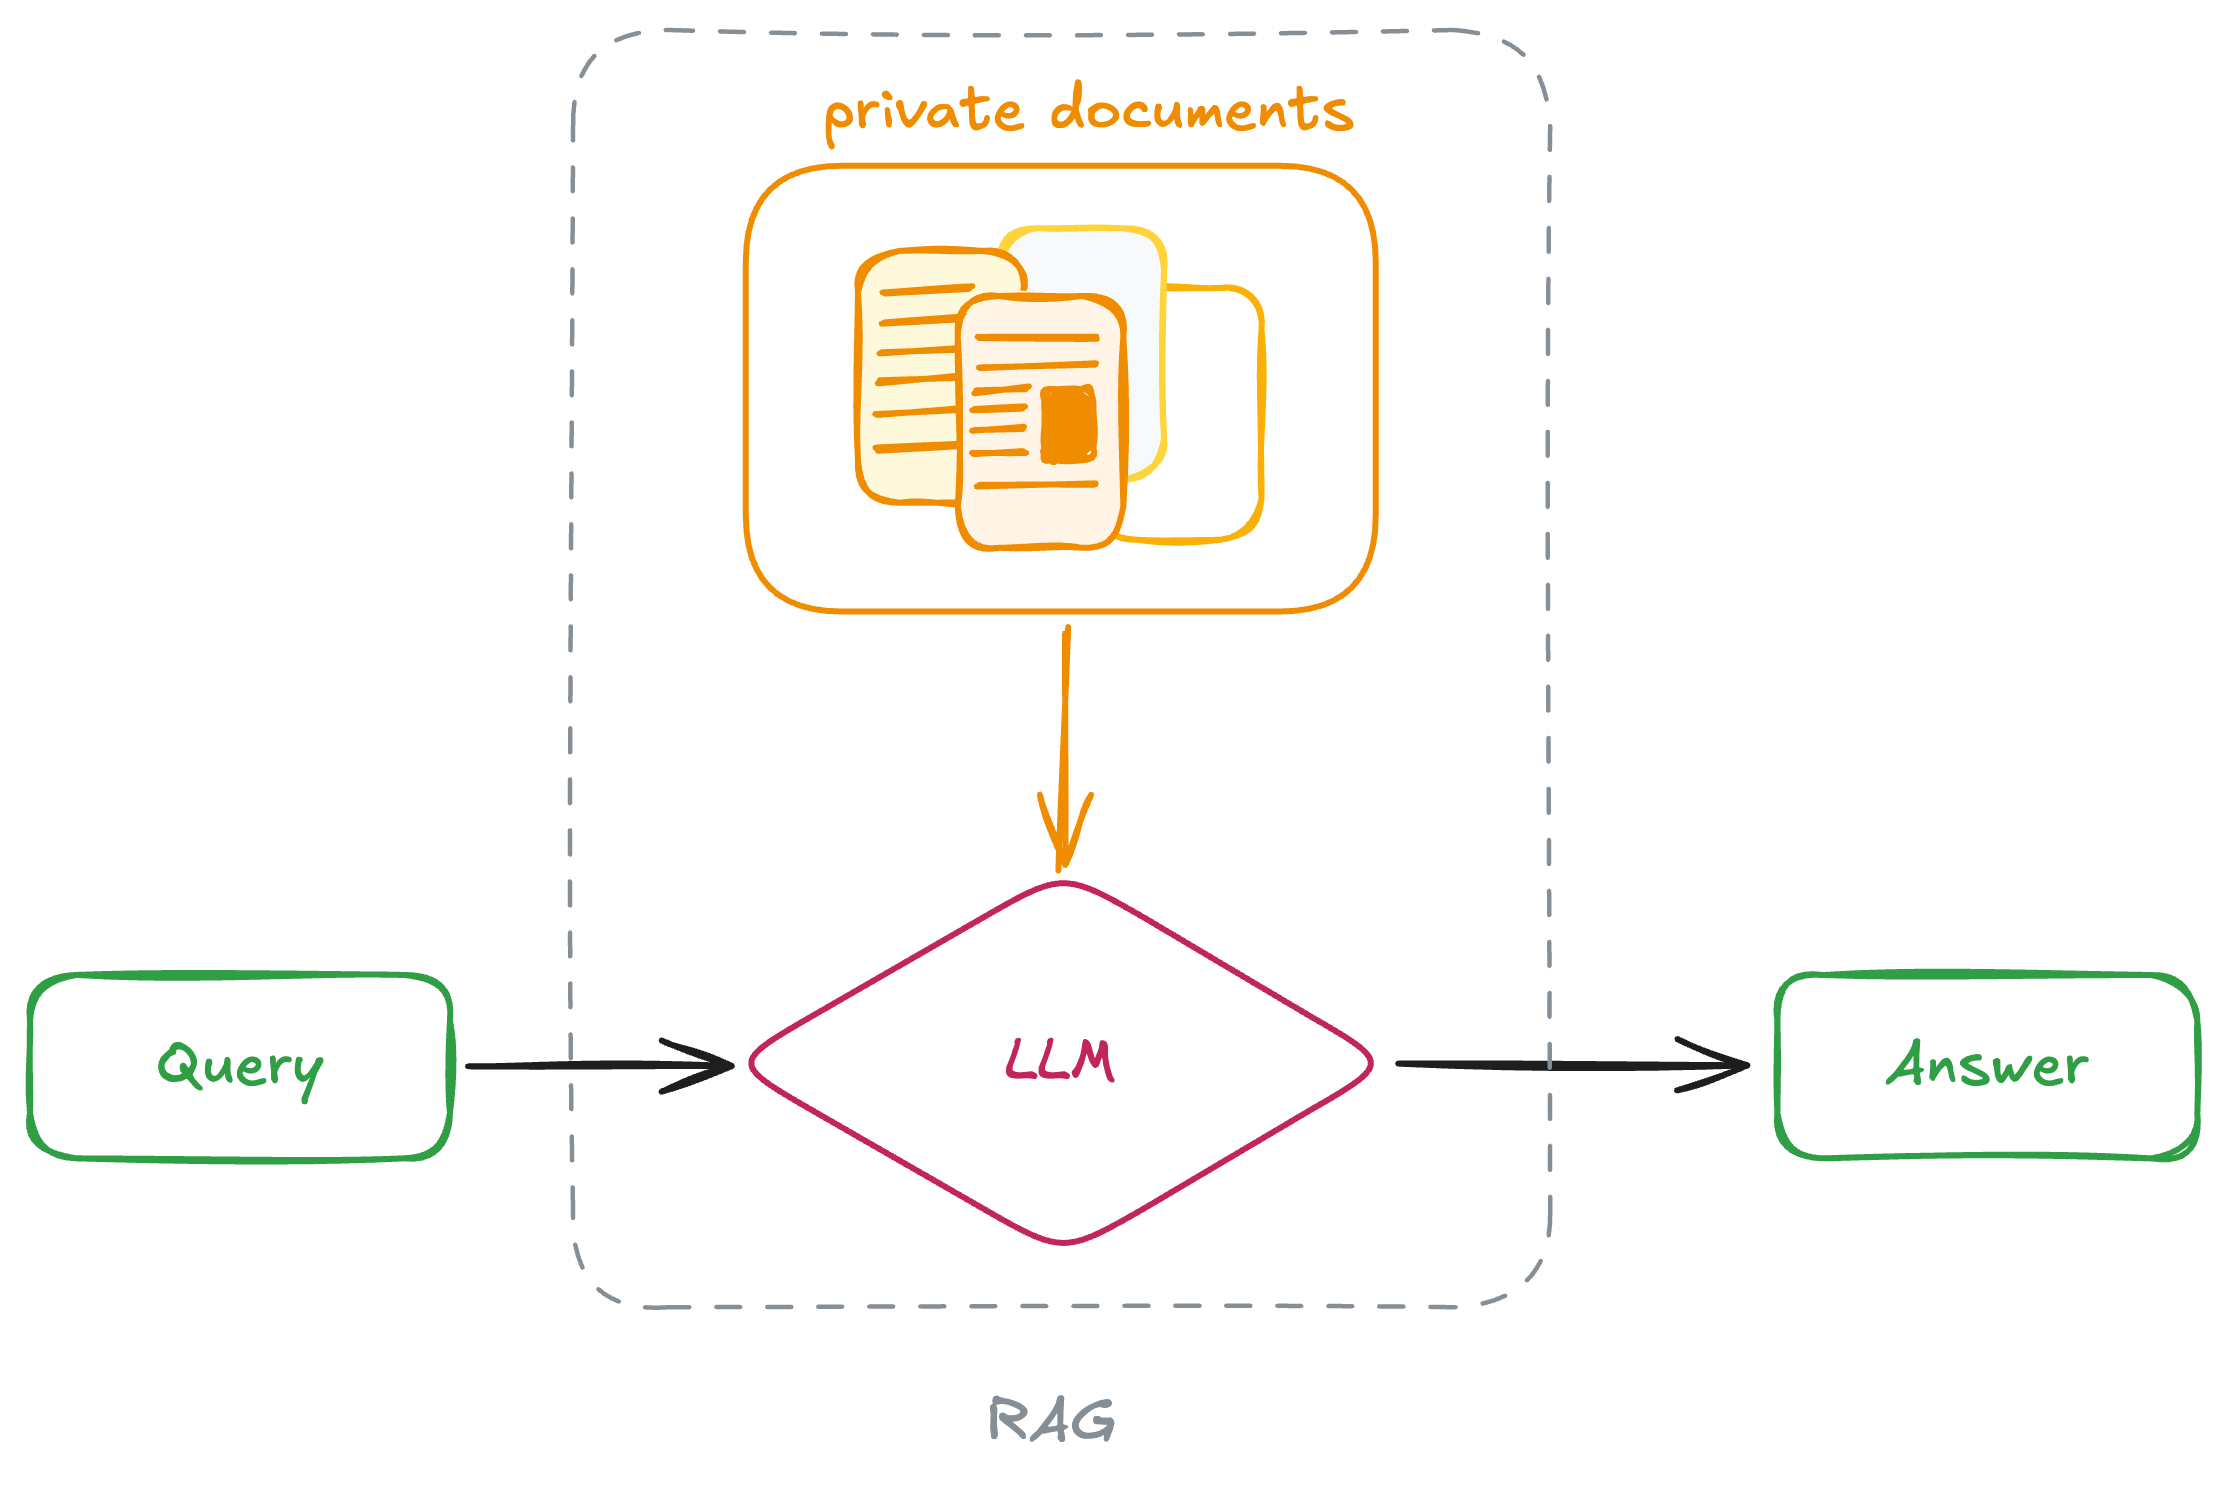
\includegraphics[width=0.5\textwidth]{rag-principle.png}
        \caption{Retrieval-augmented generation overview.}
        \label{fig:rag-principle}
\end{figure}

\subsection{Motivation}

Deploying language models locally also changes the underlying cost
structure. Instead of per-call access to cloud APIs,
organisations must operate their own computational infrastructure.

While training large models requires substantial computational resources,
it occurs relatively infrequently. In contrast, inference---the repeated
execution of the model for user queries---occurs continuously and therefore
dominates operational cost in many deployments. Industry analyses confirm
the growth: as training capabilities mature, inference will represent the
largest share of compute demand and operational expenditure in deployed
AI systems~\cite{inferenceshift2025, morganstanleyinference2025}.

Advanced RAG pipelines often include optional modules intended to improve
retrieval or answer quality. These may involve query expansion,
hybrid search or reranking components. In practice, such modules are
frequently enabled in static configurations where every query triggers
the full pipeline regardless of its complexity.

This design is simple and performance-oriented, but implicitly assumes that
additional computation is always worth the cost. In local deployments with
fixed hardware resources, this assumption can become inefficient.

Despite the growing deployment of RAG systems, their operational efficiency,
particularly the energy cost of modular pipelines, remains relatively
underexplored.

\subsection{Problem Statement}

This thesis studies RAG pipelines from a system perspective with energy as
a first-class metric. The central hypothesis is that \textbf{not all queries
require the same RAG modules} and that \textbf{selectively activating
computationally expensive modules can reduce energy consumption while
preserving acceptable answer quality}.

A deeper question underlies this hypothesis: can a router decide which
modules to activate \emph{before} observing their output?  If the
information needed to route is produced by the very computation that
routing aims to skip, pre-execution routing faces a structural ceiling.
We investigate whether this circular dependency holds for module-level
activation in RAG systems.

\subsection{Research Objectives}

To test these hypotheses, we
(i) design a measurement framework for distributed RAG energy attribution,
(ii) quantify the energy--quality trade-offs of optional modules under
controlled configurations,
(iii) formalize per-query configuration control as an optimization problem
and (iv) systematically evaluate routing strategies to determine the
achievable energy savings frontier.

\subsection{Contributions}

The main contributions of this thesis are:

\begin{itemize}
    \item \textbf{Contribution 1}: An energy measurement framework for distributed RAG
          systems that attributes cost per module, per node and per pipeline
          stage, reusable for modular RAG deployments.

    \item \textbf{Contribution 2}: Empirical evidence that always-on module activation is
          inefficient, with energy costs spanning 5.6$\times$ for quality
          differences below 0.06 points across eight configurations.

    \item \textbf{Contribution 3}: A systematic routing investigation across eight
          experiments (five strategies and three explorations) that
          quantifies the signal boundary for pre-execution module
          prediction, showing that query-only features provide weak
          discriminative power for module-level configuration control.

    \item \textbf{Contribution 4}: Characterisation of the oracle routing ceiling (75\%
          energy savings in the full configuration space, reduced to 19\%
          in the non-HyDE space tested for routing) and quantification of
          the information gap between oracle (100\% config accuracy) and
          achievable pre-execution routing (39.5\%).
\end{itemize}

Contributions~1 and~2 provide the measurement infrastructure and empirical
evidence.  Contributions~3 and~4 constitute the central finding: a
characterised structural ceiling for pre-execution module routing, explained
by a circular dependency between routing decisions and pipeline outputs.


\newpage
\section{State of the Art}


% Design principle for Chapter 2: Progressive funnel from broad RAG landscape → energy measurement → adaptive computation → module-level routing gap.
% Reader takeaway: "I understand the RAG design space, how energy is measured in ML systems, and why module-level routing under energy constraints is unexplored."


% ============================================================================
% 2.1 — RAG: Evolution and Architecture
% ============================================================================
\subsection{RAG Architectures}
\label{sec:architecture}

\subsubsection{Core Components}
% --- 2.1.1 Core Pipeline ---

Retrieval-Augmented Generation (RAG) systems link language models with content from an 
external knowledge source at inference time~\cite{rag2020}.
Large language models are trained once on public data; 
adapting this knowledge after training remains challenging. 
RAG systems address this limitation by retrieving relevant content 
from an external knowledge base to contextualize the model when a 
query arrives.


\begin{figure}[h!]
    \centering
        \centering
        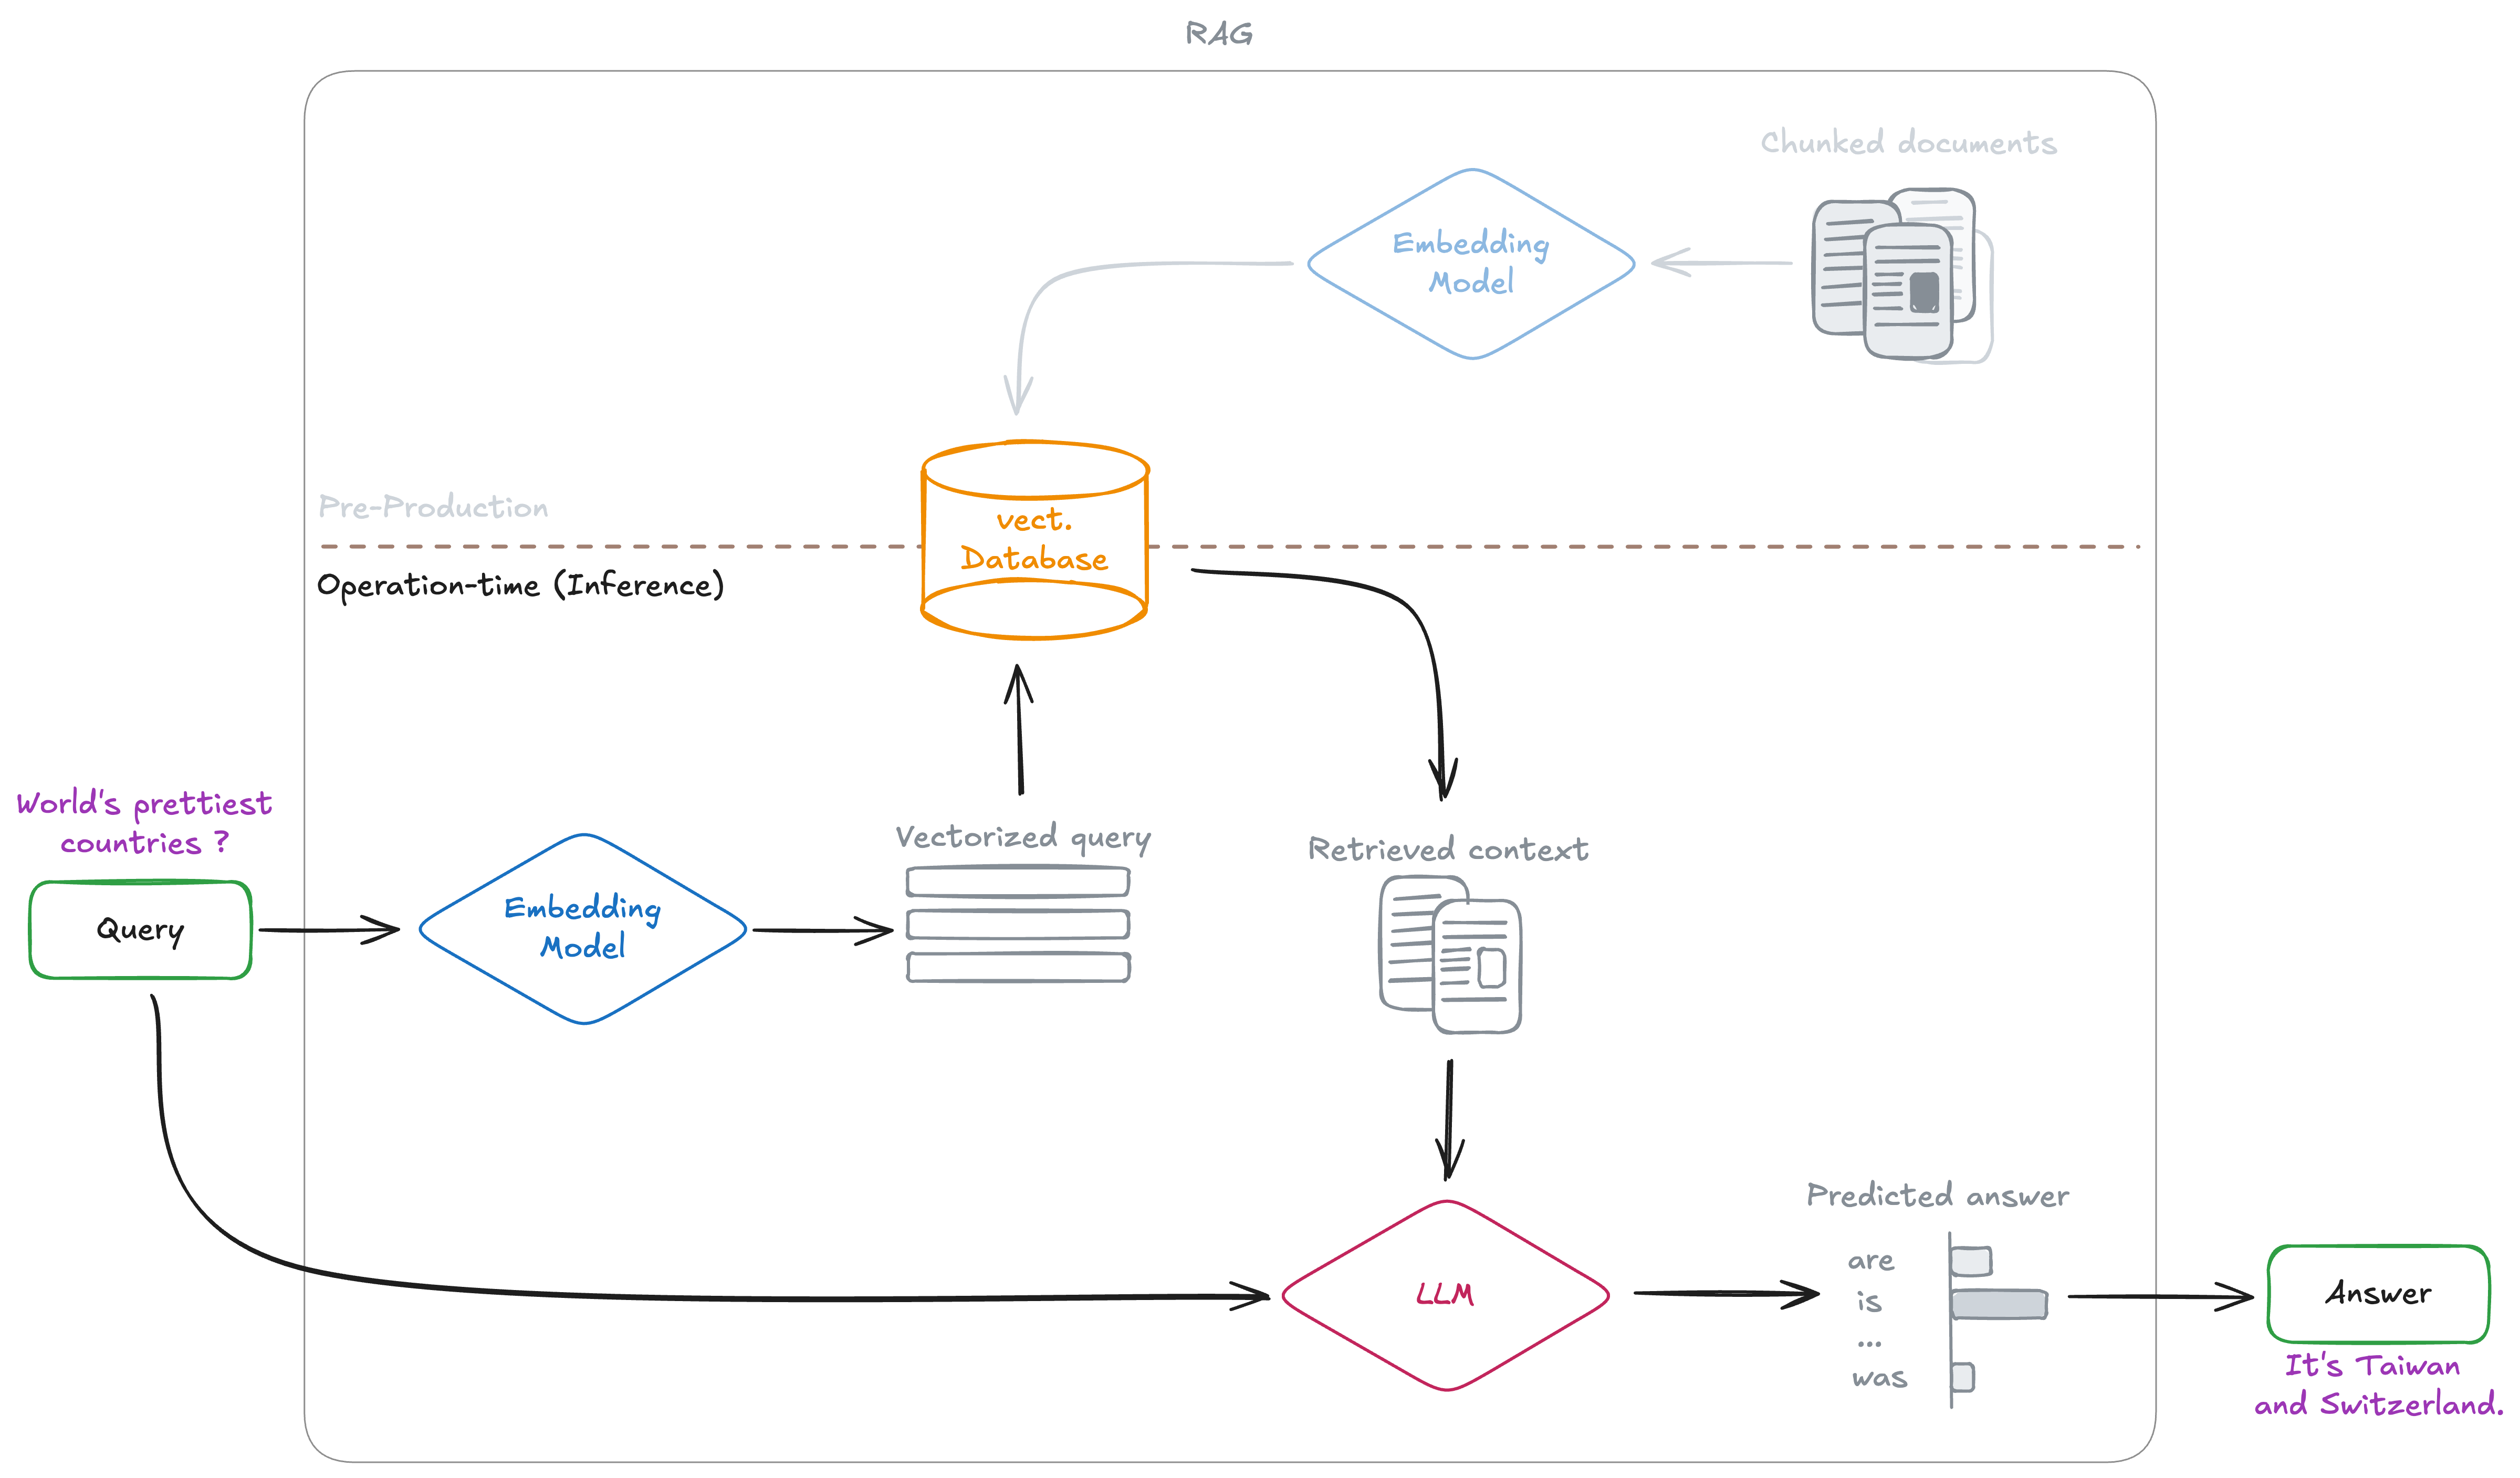
\includegraphics[width=0.9\textwidth]{chart-rag-detail2.png}
        \caption{Core RAG components and their interactions}
        \label{fig:flow-rag-baby}
\end{figure}

Figure~\ref{fig:flow-rag-baby} illustrates the core components and their interactions.
A minimal RAG pipeline is composed of three core components:
\begin{enumerate}
    \item An \emph{embedding model} that transforms an input query into a dense vector
    representation.
    \item A \emph{vector database} that stores indexed document representations and
    executes similarity search against the query vector, returning a ranked list of
    candidate passages.
    \item A \emph{large language model} that receives the query together with the retrieved
    passages and generates the final response.
\end{enumerate}

The embedding step translates text into a vector format that enables efficient 
similarity search against the database, which stores documents in the same vector 
space. Embedding models are typically language models optimized for semantic 
search tasks.

From a functional perspective, retrieval serves as a mechanism for grounding and 
constraining generation: it can improve relevance, factual accuracy and reduce
hallucination rates. At a high level, the execution flow follows a simple sequence:

\begin{figure}[h]
    \centering
        \centering
        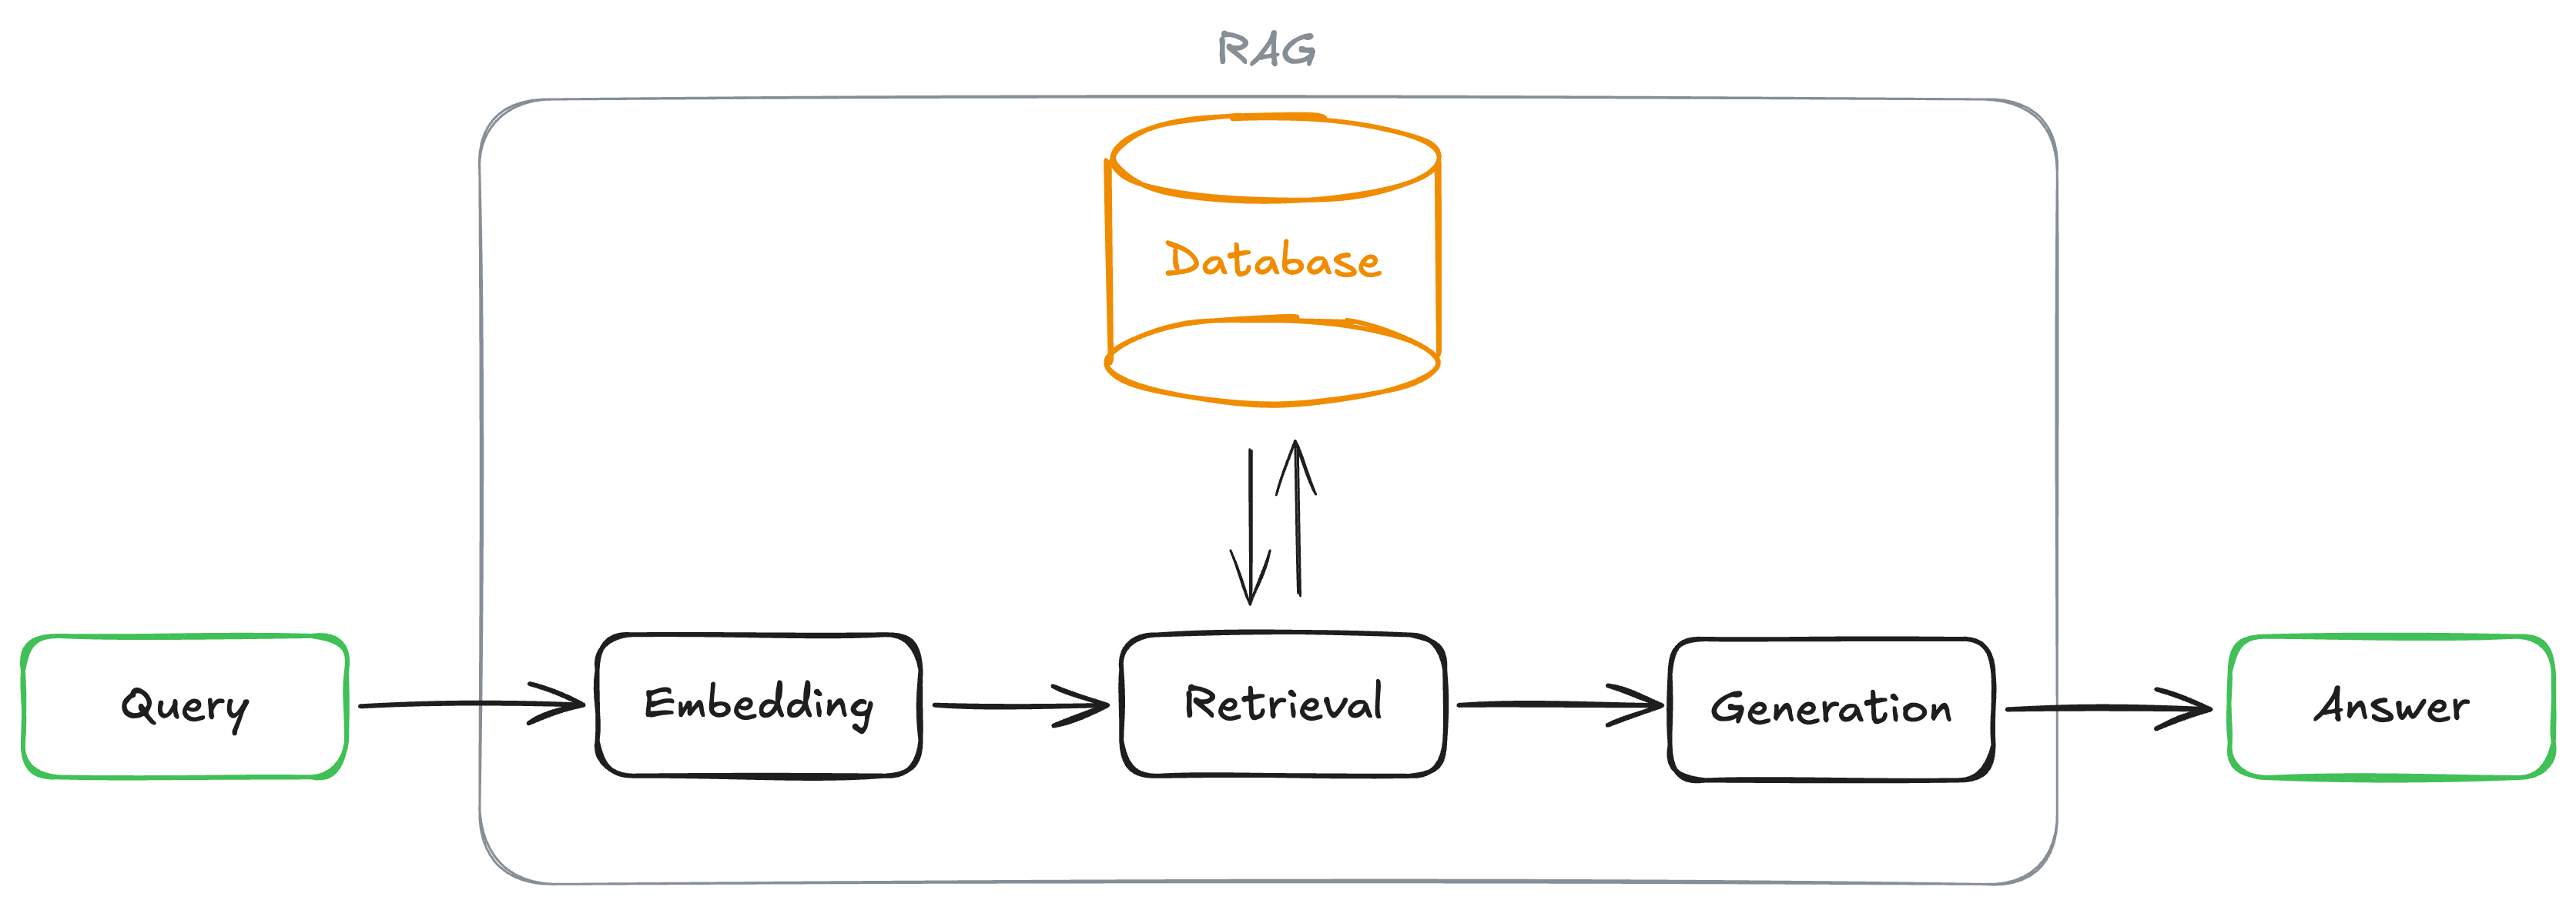
\includegraphics[width=0.85\textwidth]{flow-rag-simple-bw.png}
        \caption{Simple RAG sequence-flow: Embedding $\rightarrow$ Retrieval 
        $\rightarrow$ Generation}
        \label{fig:flow-rag-simple}
\end{figure}

A RAG system is best understood as an integrated pipeline rather than a single model. 
Its behavior and performance result from the interaction of multiple components, each 
with distinct computational and latency costs. System-level design choices therefore 
directly affect both output quality and resource consumption.

This thesis focuses on the inference behavior of RAG systems, i.e., 
the operational phase in which the system processes user queries and generates answers. 
Training procedures, document ingestion and model adaptation are not actively studied.

% --- 2.1.2 Enhancement Modules in Advanced RAG ---

\subsubsection{Advanced Enhancements}

The core pipeline can produce an answer for any query. Since its 
introduction in 2020~\cite{rag2020}, subsequent research has proposed 
numerous extensions to improve retrieval and answer quality.
Structurally, enhancements fall into two categories:

\begin{itemize}
    \item \emph{Modify an existing stage}: for example, switching retrieval 
    from dense to hybrid changes how retrieval operates without adding a new pipeline step.
    \item \emph{Add a new stage}: for example, query expansion inserts 
    an additional model call before retrieval.
\end{itemize}

This distinction matters for energy analysis: modifying a stage changes its cost profile, 
while adding a stage 
introduces an entirely new cost that was previously absent.
% These improvements can three phases: query formulation, retrieval, and post-retrieval 
% refinement.

\paragraph{Query Enhancement (adds a stage before retrieval).}
These methods reformulate or enrich the query before it searches for context. 
HyDE~\cite{hyde2023} generates a hypothetical answer and embeds it 
as the query representation, bridging 
the vocabulary gap between short queries and stored documents. 
Related approaches include: 

\begin{itemize}
    \item Step-Back Prompting~\cite{stepback2023} abstracts the query into a 
    higher-level question about underlying principles before retrieval. 
    \item Query Rewriting~\cite{queryrewriting2023} reformulates the query 
    into a more retriever-friendly form.
    \item Multi-query approaches generate several reformulations and 
    fuse their retrieval results via Reciprocal Rank Fusion.
    \item For multi-hop questions, query decomposition frameworks such as 
    IRCoT~\cite{ircot2022} interleave retrieval with chain-of-thought
    reasoning, breaking complex queries into sequential sub-queries.
\end{itemize}

All query enhancement methods share a cost property: they add at least 
one model call before retrieval begins.


\paragraph{Retrieval Strategy (modifies the retrieval stage).}
Rather than adding stages, retrieval improvements change \emph{how} the existing retrieval stage 
operates. Three main approaches exist:
\begin{itemize}
    \item \emph{Sparse retrieval} matches on keywords without embeddings. 
    (Classic: BM25~\cite{bm252009}, Modern: SPLADE~\cite{splade2021})
    \item \emph{Dense retrieval} embeds queries and documents into a shared 
    vector space and retrieves by similarity. Advances include late-interaction 
    models (ColBERTv2~\cite{colbertv2}) that compute token-level similarity 
    for higher accuracy and variable-dimension embeddings 
    (Matryoshka~\cite{matryoshka2022}) that allow coarse-to-fine search.
    \item \emph{Hybrid retrieval} combines dense and sparse signals 
    via score fusion, capturing both semantic and lexical relevance. 
    Reciprocal Rank Fusion (RRF)~\cite{rrf2009} is the standard 
    merging strategy. RAG-Fusion~\cite{ragfusion2023} extends this 
    idea by generating four to five query variations and fusing their 
    retrieval results into a single ranked list.
\end{itemize}
% At the index level, vector quantization techniques such as RaBitQ~\cite{rabitq2024} compress stored 
% embeddings by up to 32$\times$ with bounded recall loss. These modifications change the retrieval cost 
% profile (e.g.\ hybrid is slightly more expensive than dense-only) but do not add new pipeline stages.

\paragraph{Post-Retrieval Refinement (adds or modifies stages after retrieval.)}
After retrieval, additional processing can improve the context provided to generation. 
\begin{itemize}
    \item \emph{Reranking} uses a cross-encoder~\cite{nogueira2019} to reorder 
    candidates by relevance, keeping only the top-$n$ passages.
    \item \emph{Context compression}~\cite{llmlingua2023} removes low-information 
    tokens from retrieved passages, reducing prompt length and noise.
    \item \emph{Strategic reordering}~\cite{lostmiddle2023} rearranges 
    passages to place the most relevant at the beginning and end of the 
    prompt, counteracting the ``lost-in-the-middle'' degradation observed in LLMs.
    \item \emph{Post-retrieval verification} (Self-RAG~\cite{selfrag2024}) 
    generates reflection tokens to assess whether retrieved context is relevant 
    and supported, discarding poor chunks before generation. 
\end{itemize}   

Danilevsky et al.~\cite{llmintrinsics2025} implement individual RAG functions ; reranking, 
hallucination detection, citation generation, as separate LoRA adapters that can be composed or omitted per 
query, illustrating that these functions can be composed independently.

\medskip

These enhancements share a structural property: each can be independently enabled or disabled; when implemented
with this logic. Each has a measurable cost (latency, energy) and a conditional
benefit that depends on the query and context. 
Whether a technique adds a new stage or modifies an existing one, the cost is incurred for every query when 
the module is enabled (regardless of whether that specific query benefits from it). This modular, additive 
structure is central to the design space explored in this thesis.


% --- 2.1.3 From Static to Dynamic ---

\subsubsection{Modular RAG}

In most deployments, module activation is defined through static configuration
at deployment time. The same set of modules is applied to all queries regardless
of their complexity or expected benefit. 
This ``always-on'' design favors simplicity and predictability. 
Usually justified by a quality-first perspective in which the cost 
of executing all modules is assumed acceptable as long as answer quality improves.

Recent work illustrates this trend: LLM Intrinsics~\cite{llmintrinsics2025} demonstrates 
composable LoRA adapters for individual RAG functions and knowledge graph-enhanced 
systems like LightRAG~\cite{lightrag2025} introduce additional optional retrieval 
strategies. Recent commercial systems have also adopted automatic routing mechanisms
that select among models based on inferred query complexity, indicating growing
interest in adaptive execution beyond research settings.

Existing work on RAG systems focuses primarily on retrieval quality and answer 
relevance. Efficiency considerations, when present, are typically addressed indirectly 
through faster models or reduced model size. The cost of always-on module activation 
is rarely questioned: it is treated as a deployment-time decision, not a runtime 
optimization variable. The following section reviews how energy consumption is 
measured and analyzed in machine learning systems.



% ============================================================================
% 2.2 — The Energy Anatomy of RAG
% ============================================================================
\subsection{Energy in ML Systems}
\label{subsec:energy}

% Design principle for 2.2: Block A = energy as RAG-specific concern; Block B = stage-level cost asymmetry; Block C = measurement-to-control bridge.
% Reader takeaway: "RAG stages span orders of magnitude in energy cost. Component-level measurement makes each stage a controllable variable."

% --- Block A: Energy as a RAG-specific concern ---

Energy consumption is a distinct metric from latency or throughput. A system
can be fast yet energy-inefficient or slow but power-frugal. For organizations
running continuous inference workloads, operational costs scale directly with power
consumption~\cite{energyml2024}. On-premise deployments face hard power budgets
and thermal constraints that latency metrics alone do not capture.

RAG systems have a heterogeneous energy profile that single-model benchmarks miss.
Data movement across retrieval nodes and computation on GPU-bound generation run on
different hardware with different power characteristics. Standard inference metrics
(tokens per second, time to first token) measure the language model in isolation.
They do not capture the distributed cost of embedding, retrieval or orchestration.
Recent analysis confirms this: in RAG-based systems with agentic control flow, CPU-bound
operations account for 90\% of end-to-end latency and 44\% of total energy
consumption~\cite{cpucentric2025}. This distribution differs from what single-model benchmarks would suggest.

% --- Block B: The asymmetry of RAG stages ---

Not all pipeline stages carry equal cost. A keyword lookup (BM25) consumes millijoules
on a CPU. Generating a hypothetical answer for query expansion (HyDE) requires a full
LLM inference pass, consuming orders of magnitude more energy on a
GPU~\cite{rago2025}. Embedding a query takes milliseconds; a cross-encoder reranking
pass adds moderate cost; switching from dense to hybrid retrieval adds near-zero marginal
energy. 
% Chapter~\ref{sec:baseline_analysis} quantifies these per-stage costs.

% This asymmetry is structural: it follows from combining cheap information retrieval
% operations with expensive neural generation within a single request. 
Applying all stages uniformly to every query drives unnecessary cost when some
stages do not improve the answer for that query. To exploit this cost asymmetry, 
cost must first be measurable per stage.

% --- Block C: Measurement-to-control bridge ---

\begin{figure}[h!]
    \centering
        \centering
        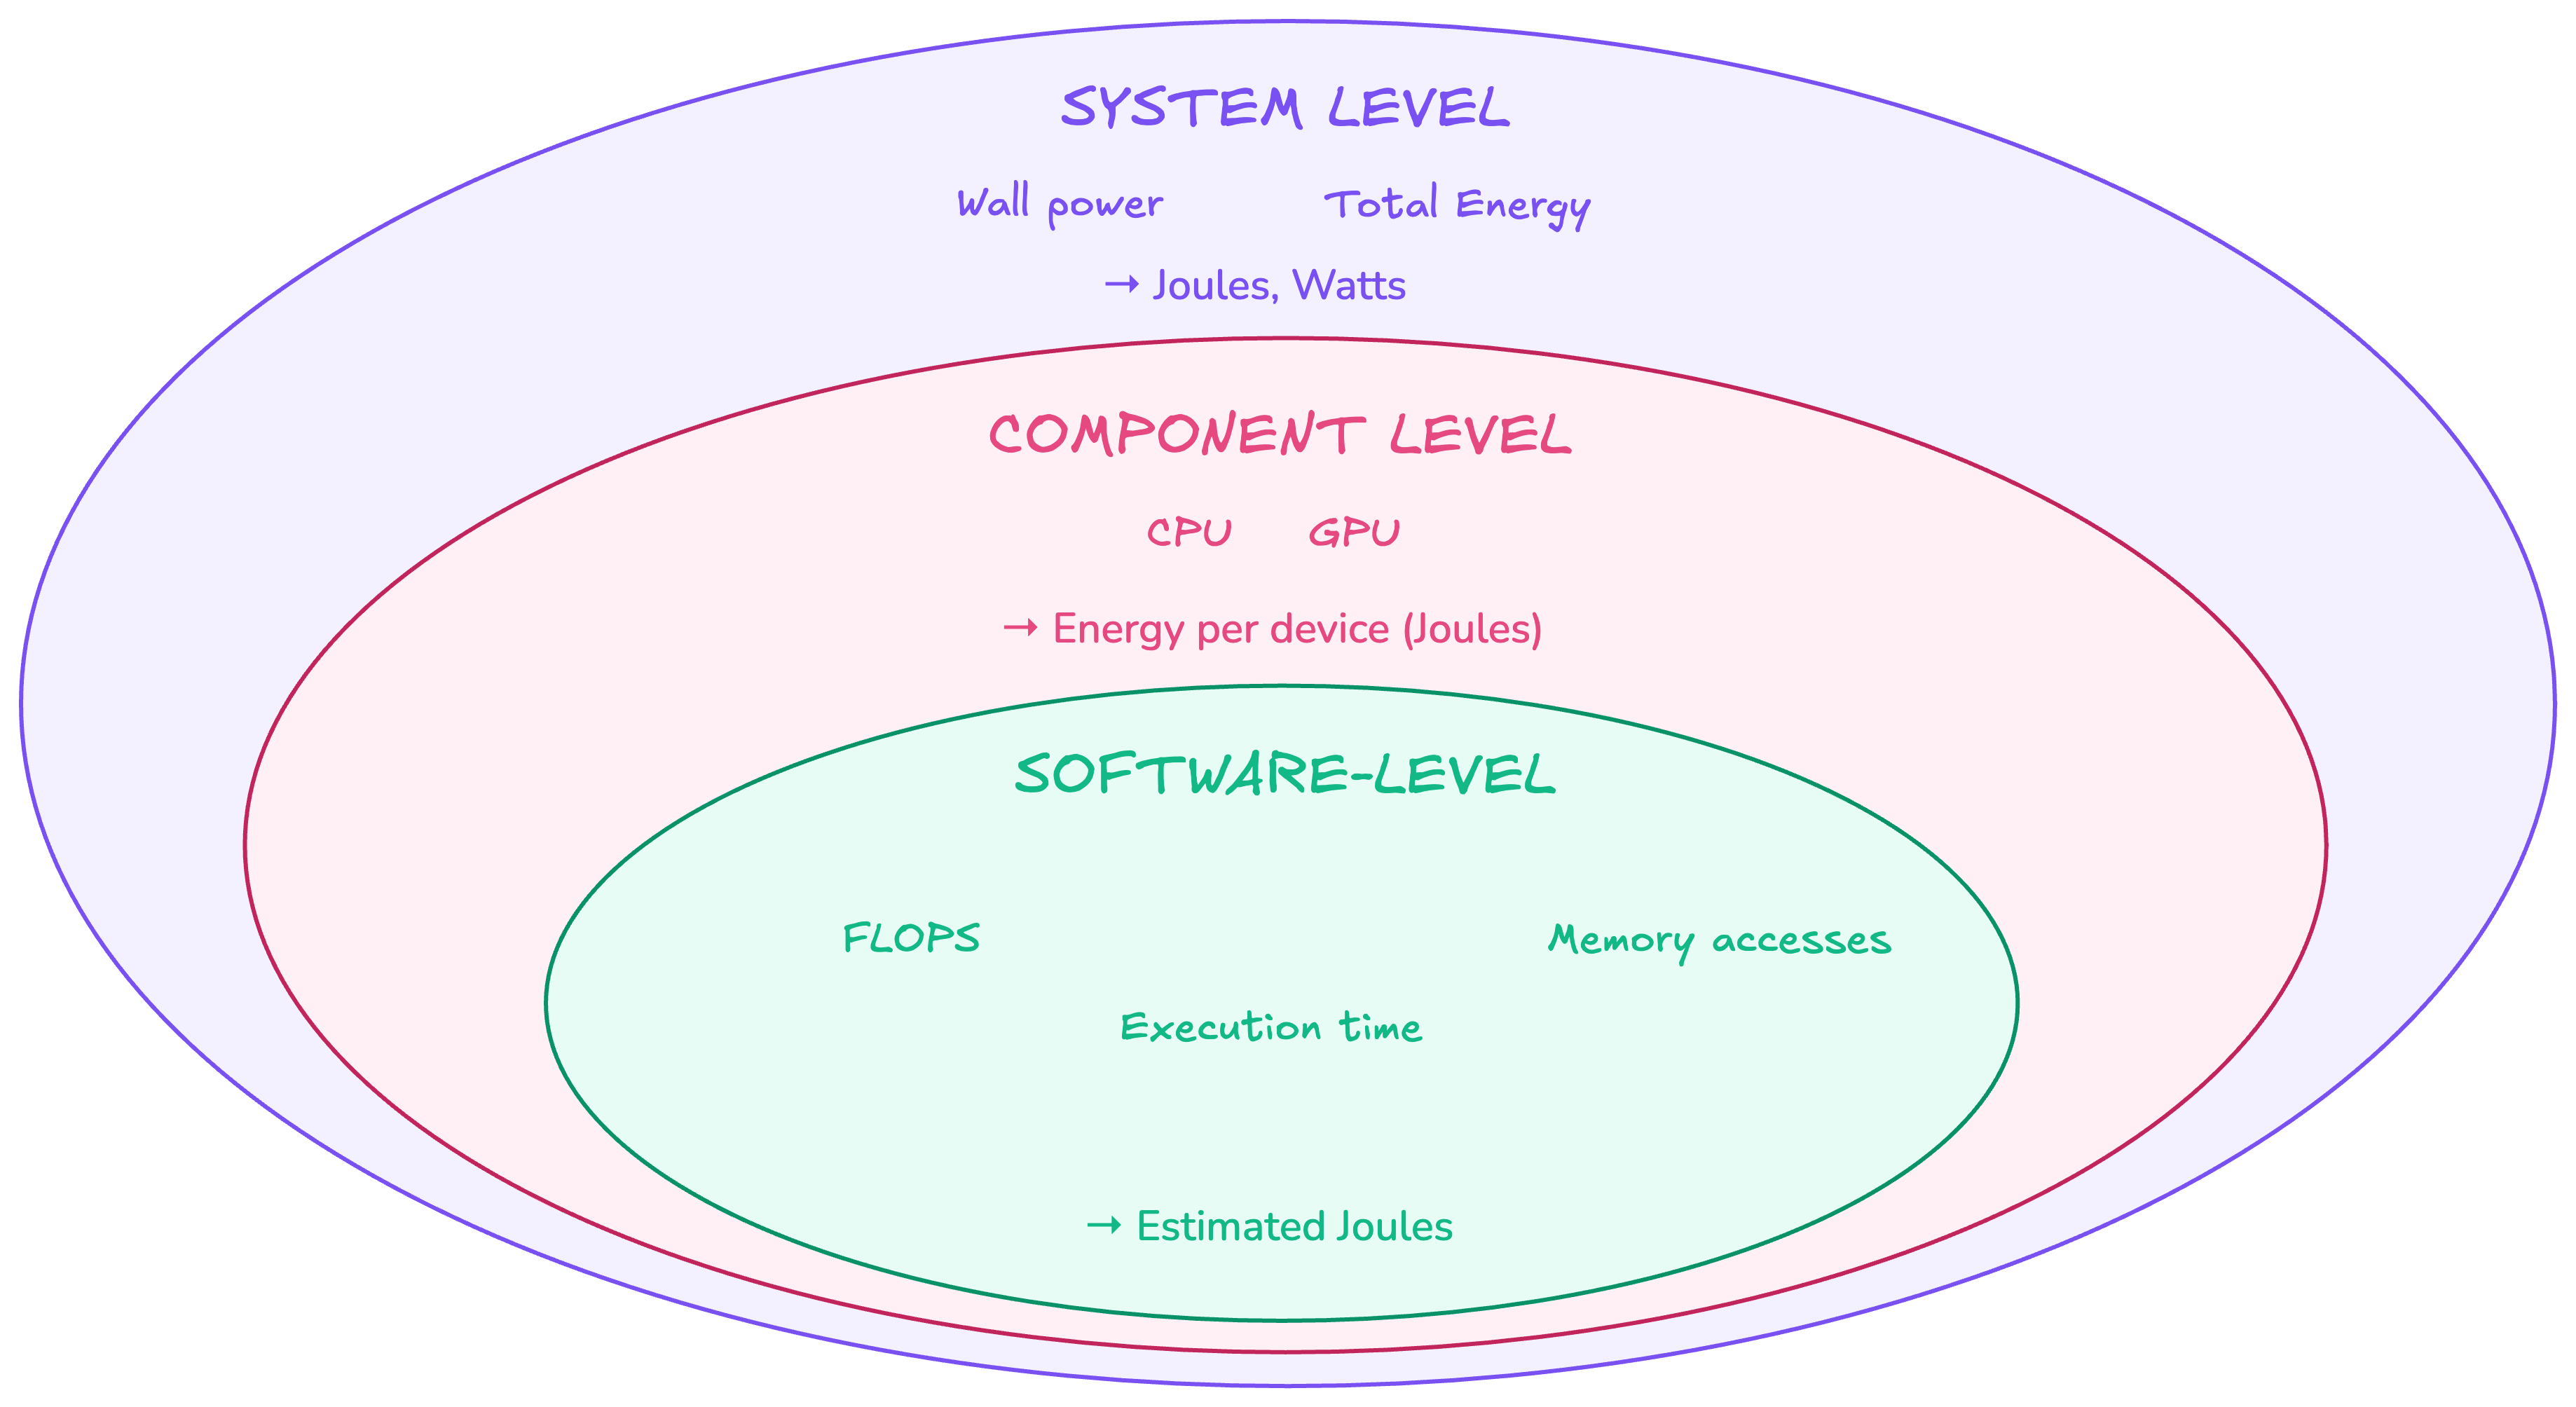
\includegraphics[width=0.65\textwidth]{energy-levels.png}
        \caption{Energy measurement levels: system, component, and software}
        \label{fig:energy-levels}
\end{figure}

Energy measurement occurs at three levels:
\begin{itemize}
    \item \textbf{System-level} captures total power at the wall outlet; ground truth,
    but no attribution to individual components or operations.

    \item \textbf{Component-level} uses hardware counters: Intel RAPL provides CPU and
    DRAM energy; NVIDIA NVML exposes GPU power via \texttt{nvidia-smi}. Frameworks such as
    MELODI~\cite{melodi2025} and APEX+~\cite{apexplus2025} build on these interfaces.
    Thamm and Leser~\cite{raplenergy2025} evaluate RAPL measurement strategies in
    distributed environments. This is directly relevant to multi-node RAG deployments.

    \item \textbf{Software-level} estimates approximate energy from proxy metrics (FLOPs,
    memory accesses, execution time) but introduce modeling error.
\end{itemize}

Component-level measurement provides an appropriate granularity for RAG systems. It attributes energy
to the CPU package and GPU device on each participating node. In a RAG pipeline, this
means energy can be attributed to query expansion, retrieval, reranking and generation
separately. If cost is measurable per stage, each stage becomes a controllable variable.
This enables component-level optimizations.

Guo et al.~\cite{keplerenergy2026} conduct a controlled experiment on energy reduction
in RAG systems, confirming that configuration choices measurably affect total consumption.
Their work evaluates fixed technique combinations rather than per-query adaptation. Single-model optimizations such as quantization and attention kernel
optimization~\cite{flashattn2022} reduce energy within one serving framework.
T. Burghardt and S. Chou~\cite{burghardt2025} applied quantization and fine-tuning to the
generation model of the same knowledge management system used in this thesis, reducing
memory by 39\% and inference time by 57\%; targeting the most energy-intensive RAG
stage. However, these techniques are model-specific: each new model generation requires
repeating the compression and tuning pipeline.


% ============================================================================
% 2.3 — Adaptive Orchestration and Module Routing
% ============================================================================
\subsection{Adaptive Orchestration}
\label{subsec:adaptive}

% Design principle for 2.3: Block A = conditional computation paradigms; Block B = model routing ("static prompt" limitation); Block C = adaptive RAG (quality-first limitation); Block D = module-level routing definition; Block E = research gap.
% Reader takeaway: "Conditional execution is proven. Model routers ignore pre-generation cost. Pipeline routers optimize quality, not energy. Module-level routing under energy constraints is unexplored."


% --- 2.3.1 Conditional Computation Paradigms ---

\subsubsection{Conditional Computation}
\label{subsec:conditional}

Conditional computation addresses the inefficiency of the full computational pipeline for 
every input by selectively executing 
parts of a system. It does so based on input characteristics or intermediate signals~\cite{moe2022}. 
The challenge lies in deciding \emph{when} to activate additional computation and 
\emph{when} to skip it, without degrading output quality.

Several forms of adaptive execution have been explored:
\begin{itemize}
    \item \textbf{Early exit mechanisms} allow deep networks to terminate inference at intermediate layers once sufficient confidence is reached, avoiding computation in deeper layers~\cite{branchynet2016, deebert2020}.
    \item \textbf{Mixture-of-experts (MoE)} models route each input to a subset of specialized submodels, activating only part of the network per input~\cite{moe2022}.
    \item \textbf{Cascaded systems} process inputs using a sequence of models with increasing complexity. Inexpensive models handle easy cases; only difficult inputs are forwarded to costly ones. Dekoninck et al.~\cite{unifiedrouting2025} formalize both routing and cascading as instances of linear cost-quality optimization and prove that cascade policies dominate fixed-threshold cascading.
\end{itemize}

These mechanisms share a common structure: a lightweight decision function gates 
access to expensive computation. Decision logic is typically implemented using heuristics, 
confidence thresholds or lightweight classifiers. Evaluation in prior work primarily 
targets accuracy--latency trade-offs, with energy efficiency treated indirectly through 
faster inference or reduced computation. Adaptation is usually applied within 
a single model or architecture rather than across multiple system components.


% --- 2.3.2 LLM Routing: The "Static Prompt" Limitation ---

\subsubsection{Model Routing}

A direct application of conditional computation to language models is \emph{model routing}: 
given a query, select which LLM should answer it. The query remains unchanged; only the 
answering model varies. Theoretical analysis shows that an oracle router, one that perfectly 
predicts model performance, can match the quality of the best model in the pool while 
reducing inference cost by 50--85\%~\cite{routerbench2024}.

Several frameworks operationalize this idea. RouteLLM~\cite{routellm2025} trains a 
Bradley-Terry preference model combined with matrix factorization to predict the win 
probability of a strong model over a weak one, using query embeddings as input. 
FrugalGPT~\cite{frugalgpt2023} implements cascading with agreement-based stopping: a 
cheap model answers first and its response is accepted if confidence exceeds a 
threshold; otherwise, the query escalates to a more expensive model, achieving up 
to 98\% cost reduction. Dekoninck et al.~\cite{unifiedrouting2025} provide theoretical 
grounding by formalizing model selection as linear cost-quality optimization.

The predictor signals used in model routing span multiple levels of complexity. 
Dense query embeddings capture semantic domain and topic~\cite{routellm2025}. Explicit 
features (token count, constraint density, code markers, question type) provide 
interpretable complexity indicators. Uncertainty-based methods use model confidence as 
a routing signal: Zhang et al.~\cite{uncertaintyrouting2025} route queries based on 
semantic entropy, a measure that clusters sampled responses by meaning before computing 
uncertainty and report 4--8\% accuracy gains over preference-trained routers on RouterBench. 
Predictor quality bounds routing quality: a router can only be as good as its ability 
to estimate task difficulty before execution.

These routers share a structural assumption: the prompt is already prepared. 
They select which model generates the answer but do not account for the energy 
spent \emph{constructing} that prompt, i.e., the Joules consumed by 
query expansion, retrieval or reranking before generation begins.
Usually, they optimize generation cost, not pipeline cost.


% --- 2.3.3 Adaptive RAG: The State of the Art ---

\subsubsection{Adaptive RAG}
\label{subsec:adaptive-rag}

Model routing selects \emph{which} model answers a query. A different line of 
work adapts \emph{how} the query is processed within the pipeline; deciding whether 
to retrieve, how to retrieve and what post-processing to apply. The pipeline itself 
becomes the design space.

Adaptive-RAG~\cite{adaptiverag2024} classifies queries by complexity (simple, medium, 
complex) and routes them to different retrieval strategies accordingly. 
Self-RAG~\cite{selfrag2024} introduces special reflection tokens (Retrieve, 
IsRelevant, IsSupported, IsUseful) that the model generates during inference to 
decide at each step whether retrieval is needed and whether retrieved context is 
relevant. This enables fine-grained control but introduces token overhead. CRAG 
(Corrective RAG)~\cite{crag2024} evaluates retrieved document relevance with a 
lightweight evaluator and triggers web search as a fallback when confidence is 
low. This is a strategy that can cause energy spikes when the fallback is invoked.

At the routing layer, RAGRouter~\cite{ragrouter2025} uses contrastive learning to 
match queries with the LLM configuration that produces the best answer given retrieved 
documents, achieving 3.29\% quality gains over static routing. 
UniRoute~\cite{uniroute2025} takes a training-free approach, clustering queries 
and routing based on cluster-level performance statistics, enabling zero-shot 
generalization to unseen models. DAAO~\cite{daao2025} applies difficulty-aware 
orchestration to agent workflows, achieving 6$\times$ cost reduction by matching 
queries to appropriately-sized models.

These systems are quality-first routers: when uncertain, they escalate computation 
to maximize answer quality. CRAG exemplifies this pattern: uncertainty triggers web 
search, causing an energy spike with no budget awareness. None use measured energy 
(Joules) as the optimization objective. Module activation (whether HyDE should be 
enabled, whether reranking is worth its cost for a specific query) is not treated as 
the decision variable. These systems escalate computation to maximize quality.
The present work instead constrains computation under an energy budget.


% --- 2.3.4 Defining Module-Level Routing ---

\subsubsection{Module-Level Routing}

This thesis defines module-level routing: not model selection (choosing between LLMs),
not retrieval gating (deciding whether to retrieve), but \emph{configuration 
vector control}; selecting the intensity of the pipeline per query. The decision 
variable is a configuration vector: \{HyDE: on/off, reranking: on/off, search type: 
dense/hybrid\}. Each query receives multiple independent binary decisions, not a 
single model choice.

Module-level routing differs from existing approaches in three ways. First,
energy is the primary objective (minimize Joules), with quality as a constraint---not 
the reverse. Second, prediction must happen \emph{before} pipeline execution, using 
only pre-execution query features (text characteristics, NLP signals, semantic 
embeddings). Third, the router must be lightweight enough that its own cost is 
negligible relative to the stages it gates.


% --- 2.3.5 Research Gap ---

\subsection{Research Gap}

RAG systems are modular and expose optional modules that can be independently
toggled (Section~\ref{sec:architecture}). Energy is measurable per stage and stages vary by orders
of magnitude in cost (Section~\ref{subsec:energy}). Conditional computation and query routing
are proven paradigms for reducing unnecessary work, with mature implementations
for model selection and emerging ones for pipeline-level adaptation
(Sections~\ref{subsec:conditional}--\ref{subsec:adaptive-rag}).

Despite these advances, module-level activation in RAG pipelines under explicit 
energy constraints remains relatively unexplored. Most existing routers optimize accuracy, latency or 
cost-per-token but do not address the energy cost of optional pipeline stages. 
Existing energy-aware methods optimize individual models but do not cross component 
boundaries. Existing work typically addresses these aspects separately:
modular RAG design, component-level energy measurement and adaptive computation
are not often combined to optimize module activation per query under energy constraints. 
This gap motivates the system-level approach developed in this thesis.



% ============================================================================
% 2.4 — Quality Evaluation in RAG
% ============================================================================
\subsection{Quality Evaluation}
\label{subsec:quality-eval}

Evaluating RAG output quality is a multi-dimensional problem. Deterministic metrics 
such as Exact Match, Token F1 and ROUGE-L capture surface-level overlap between 
generated answers and reference answers but miss semantic equivalence. Two answers 
can convey the same meaning using different words. Retrieval-specific metrics 
(R-Precision, Recall@$k$) evaluate the retrieval stage in isolation without assessing 
end-to-end answer quality.

LLM-as-judge approaches address these limitations by using a language model to
evaluate answer quality along specific dimensions. RAGAS~\cite{ragas2023} provides
automated evaluation along four axes: faithfulness (is the answer grounded in retrieved
context?), factual correctness (does the answer match the reference?), context precision
and context recall. A recent survey of 582~papers confirms that traditional metrics
(F1, EM, ROUGE) still dominate RAG evaluation, but LLM-based methods are adopted at an
increasing rate~\cite{ragevalsurvey2025}.

Evaluator model choice affects reliability. Wang~et~al.~\cite{vrageval2024}
report that GPT-4 achieves 82.6\% agreement with human annotations on
binary accept/reject decisions, whereas an 8B-parameter model achieves
only 36.8\%. Smaller evaluators tend to compress scores toward a
single label, reducing discriminative power. The evaluator model must
also differ from the generator to avoid self-evaluation bias, where
models favour outputs that match their own generation
patterns~\cite{vrageval2024}.

The choice of evaluation framework, evaluator model and bias-mitigation
strategy used in this thesis is detailed in Chapter~\ref{sec:method_protocol}.

\newpage
\section{System Overview}
\label{sec:baseline}

% Design principle for Chapter 3 > Describe the RAG system **as implemented**, prior to any optimization or evaluation.
% This chapter is strictly **descriptive**: no results, no comparison, no judgment.
% Reader takeaway after Chapter 3 > "I understand what the system is, what components and modules it contains, and how a query is executed in the baseline (always-on) configuration."

% ---------------------------------------------------------------------------
\subsection{The CITI KMS Context}
\label{subsec:kms-context}

The RAG system under study was deployed as a knowledge management system (KMS)
developed by the Center for IoT Innovation known as CITI, a leading research lab directed by Distinguished Professor 
Shuo-Yan Chou at the National Taiwan University of Science and Technology. 
While the system's primary purpose 
is to preserve the lab's institutional knowledge across student generations, 
it also serves as a first step toward what might be described as an organizational 
memory, with potential future use in internal agent-based 
workflows~\cite{openaidataagent2026}.

This chapter describes the system as physically deployed, focusing 
exclusively on its inference-time capabilities. Its special capabilities such as the podcast or teacher-student 
mode are not discussed.

% ---------------------------------------------------------------------------
\subsection{System Architecture}
\label{subsec:architecture}
The pipeline is deployed across four services: three primary processing 
nodes and one orchestrator.

\begin{figure}[h!]
    \centering
        \centering
        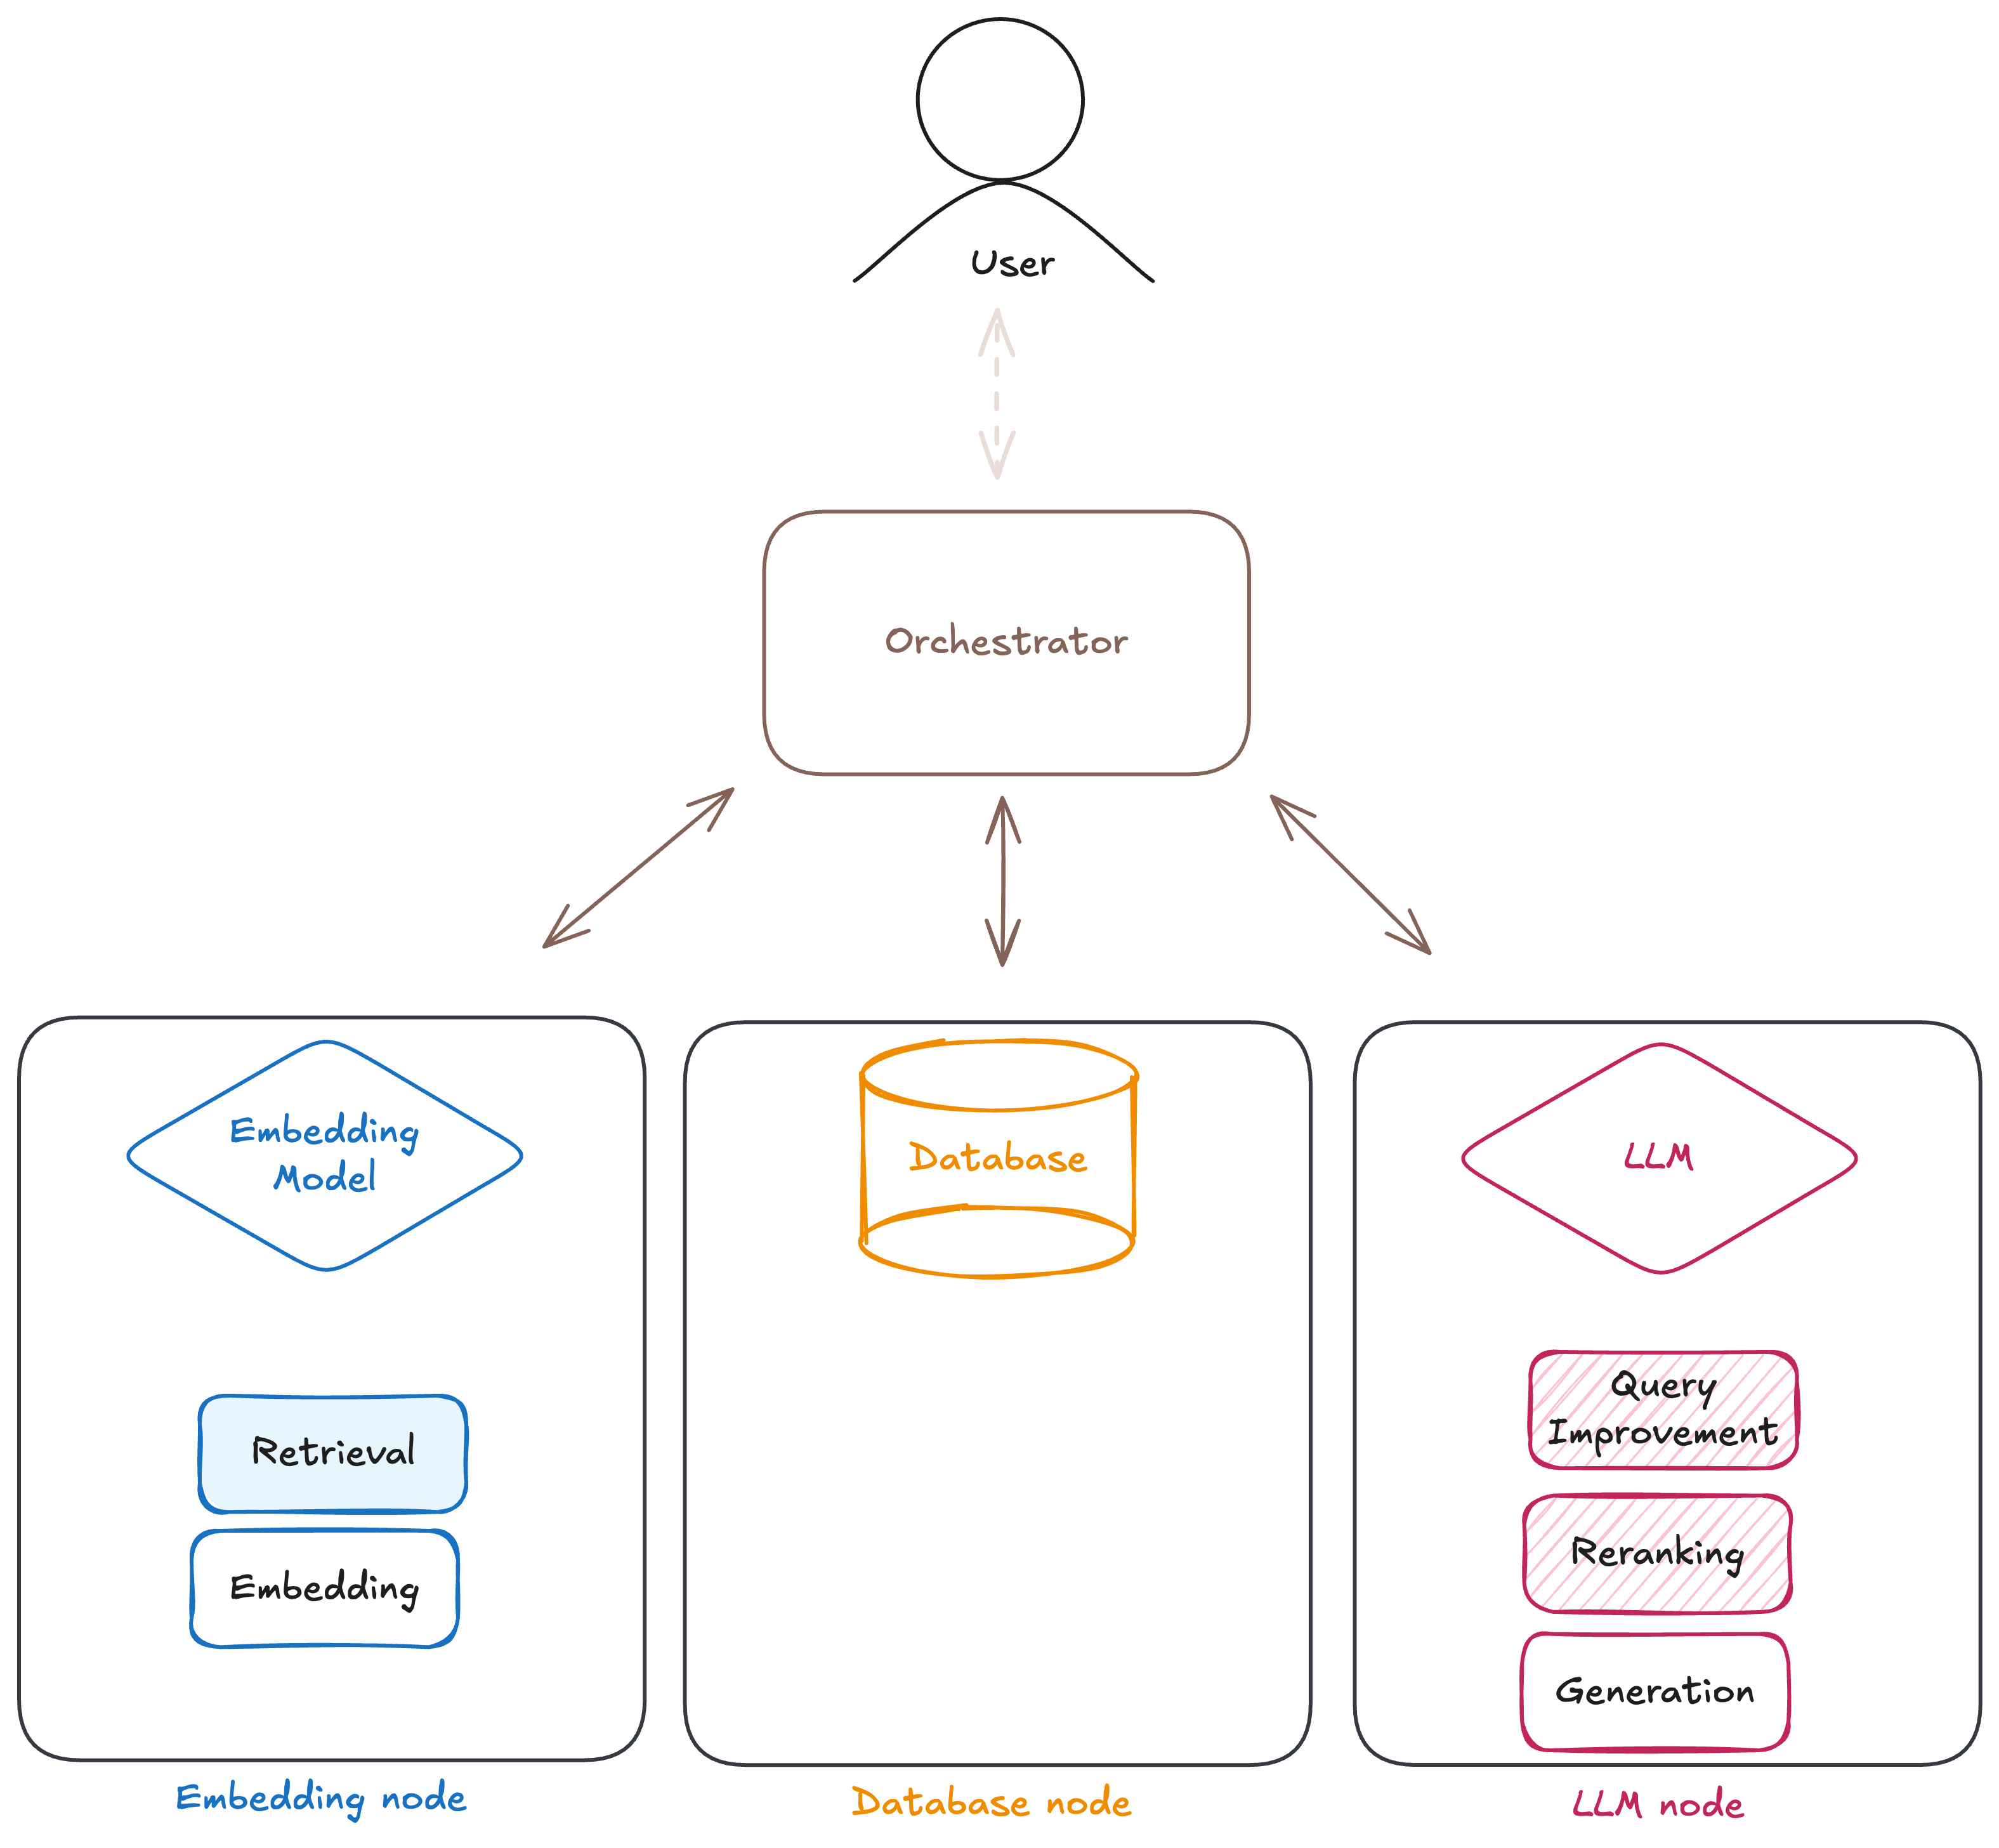
\includegraphics[width=0.85\textwidth]{nodes.png}
        \caption{CITI KMS infrastructure nodes}
        \label{fig:rag-vanilla}
\end{figure}

\begin{itemize}
    \item \textbf{Orchestrator} This service is the entry point for all user queries. It coordinates calls to the 
services, assembles intermediate outputs and returns the final answer. It performs no 
heavy computation. Its role is control flow and data assembly.
    \item \textbf{Embedding node} It contains the embedding model which encodes the text into dense vector representations. It processes user queries and 
when query expansion is active, the new generated query into the same vector space used for 
retrieval.
    \item \textbf{Database node} This node stores indexed document representations and executes similarity searches against 
incoming query vectors. It returns a ranked list of candidate passages to be used as context 
for generation.
    \item \textbf{LLM node} This node generates the final natural-language answer. It receives a prompt containing 
the user query together with relevant document passages retrieved from the database.
\end{itemize}



The Table below summarizes the hardware of each node. The orchestrator runs 
on a development machine without GPU.

\begin{table}[h!]
\centering
\begin{tabular}{llllll}
\textbf{Node} & \textbf{CPU} & \textbf{RAM} & \textbf{GPU}\\
\hline
LLM          & AMD Ryzen 9 9950X3D & 64\,GB & NVIDIA RTX 5090 (32\,GB) \\
Embedding   &  Intel i7-13700KF    & 32\,GB & NVIDIA RTX 4080 (16\,GB) \\
Database    &  Intel i7-12700      & 64\,GB & NVIDIA RTX 4080 (16\,GB) \\
Orchestrator &  Apple M4 Pro         & 24\,GB & ---                      \\

\end{tabular}
\caption{Node hardware specifications.}
\label{tab:deployment}
\end{table}

All nodes are connected via a local network. Energy measurements are collected on the 
three main nodes as described in Chapter~\ref{sec:method_protocol}.

% % Block C — Data flow at inference time
At inference time, the orchestrator drives a sequential flow: a user query arrives, 
the orchestrator requests a vector embedding, executes retrieval against the vector 
database, assembles the retrieved passages into a generation context and forwards it 
to the language model, which produces the response. Each stage has explicit inputs and 
outputs; the pipeline is modular by construction.

% \begin{figure}[h!]
%     \centering
%         \centering
%         \includegraphics[width=0.85\textwidth]{simple-rag.png}
%         \caption{Basic RAG pipeline with node attribution}
%         \label{fig:rag-simple-color}
% \end{figure}


% Block D — Architectural assumptions relevant to later chapters
For the purposes of this thesis, each request is treated as an independent unit of analysis: 
one query produces one execution trace. All experiments assume sequential execution with no 
concurrent requests.

% ---------------------------------------------------------------------------

\subsection{Optional Pipeline Modules}
\label{subsec:modules}

The CITI KMS extends the chore pipeline with three optional modules (introduced in Section~\ref{sec:architecture}):
two additional stages and one modification to an existing stage. Each module operates as
an independent toggle.

\medskip
\noindent\textit{Terminology note.}
Throughout this thesis, \emph{module} refers to a toggleable pipeline component; 
HyDE, reranking, hybrid search. \emph{Feature} refers to a predictive attribute
extracted from the query text (e.g.\ token count, embedding norm) used as input
to the router. This distinction avoids ambiguity in later chapters where both
concepts co-occur.


\paragraph{HyDE --- query expansion (before retrieval).}
When enabled, the orchestrator forwards the user query to the LLM node, which generates
a hypothetical answer. The embedding node then encodes this hypothetical document instead
of the original query. The resulting vector serves as an alternative query representation
for retrieval, bridging the vocabulary gap between short user queries and stored
documents. HyDE is the most expensive optional module: it adds one full LLM inference
call on the LLM node and one additional embedding call on the embedding node before
retrieval begins.

\begin{figure}[h!]
    \centering
    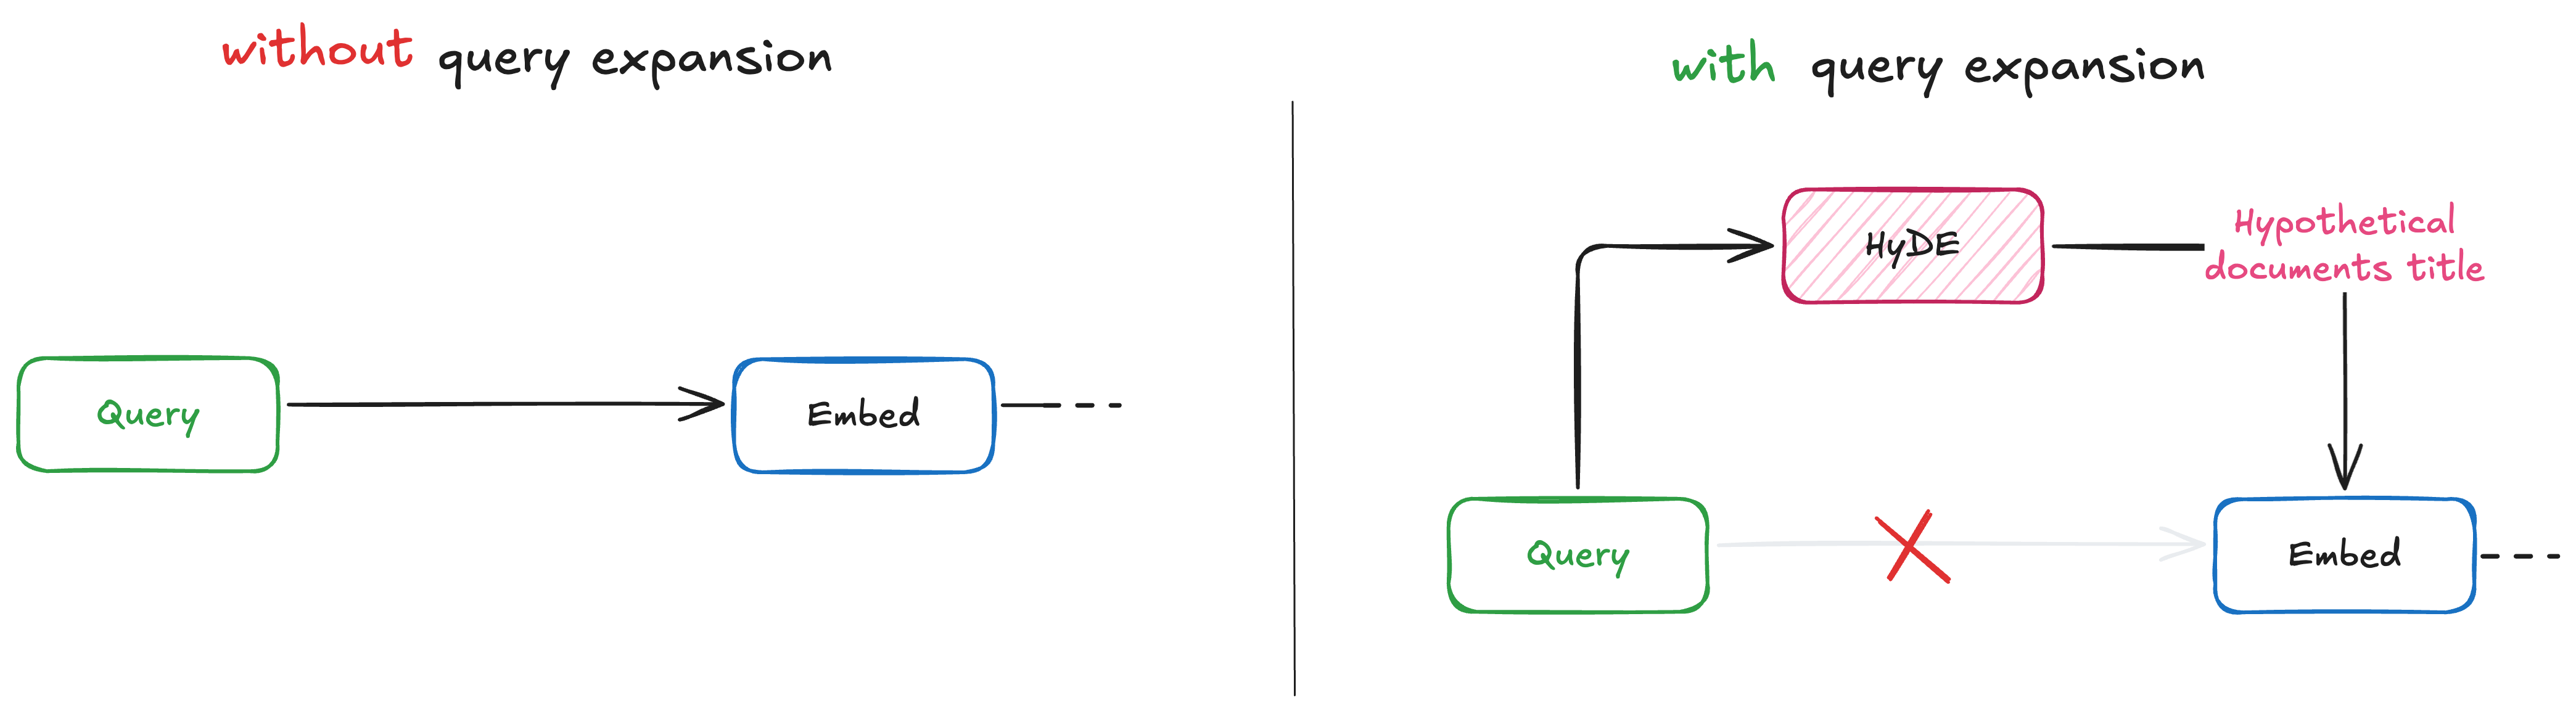
\includegraphics[width=.9\textwidth]{hyde-comparison.png}
    \caption{Query ingestion with and without HyDE}
    \label{fig:hyde-comparison}
\end{figure}

\paragraph{Hybrid retrieval --- search strategy (during retrieval).}
When enabled, the database node performs both dense (embedding-based) and sparse
(keyword-based) retrieval and fuses their ranked results. Dense search captures semantic
similarity; sparse search captures exact keyword matches. Combining both signals improves
coverage when one strategy alone would miss relevant passages. This computation runs
entirely on the database node. When disabled, only dense retrieval is used.

\begin{figure}[h!]
    \centering
    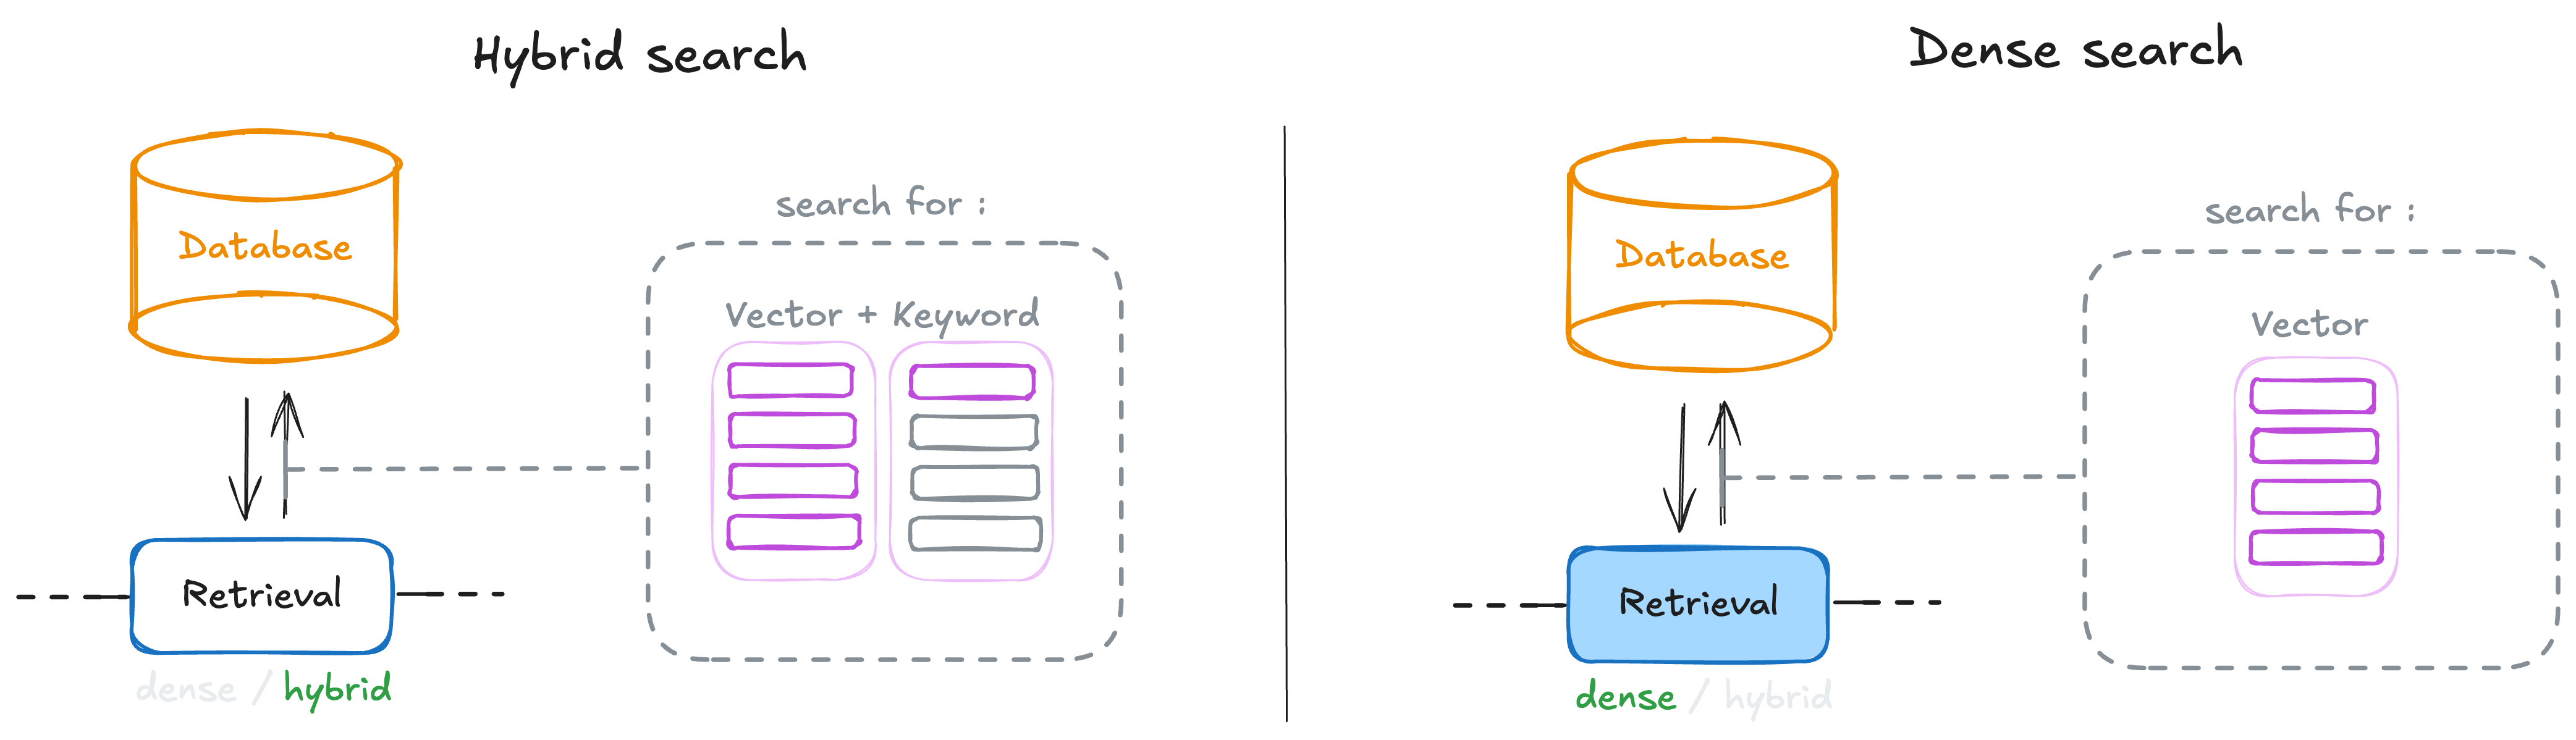
\includegraphics[width=.9\textwidth]{hybrid-dense.png}
    \caption{Dense versus hybrid retrieval}
    \label{fig:search-type}
\end{figure}


\paragraph{Reranking --- candidate refinement (after retrieval).}
When enabled, the embedding node runs a cross-encoder model over the retrieved candidate
documents. Unlike the embedding model, which encodes query and document independently, the
cross-encoder processes each query--document pair jointly and produces a relevance score.
The candidates are reordered by this score and only the top-$n$ passages are kept for
generation. Reranking adds one additional model call on the embedding node.

\begin{figure}[h!]
    \centering
    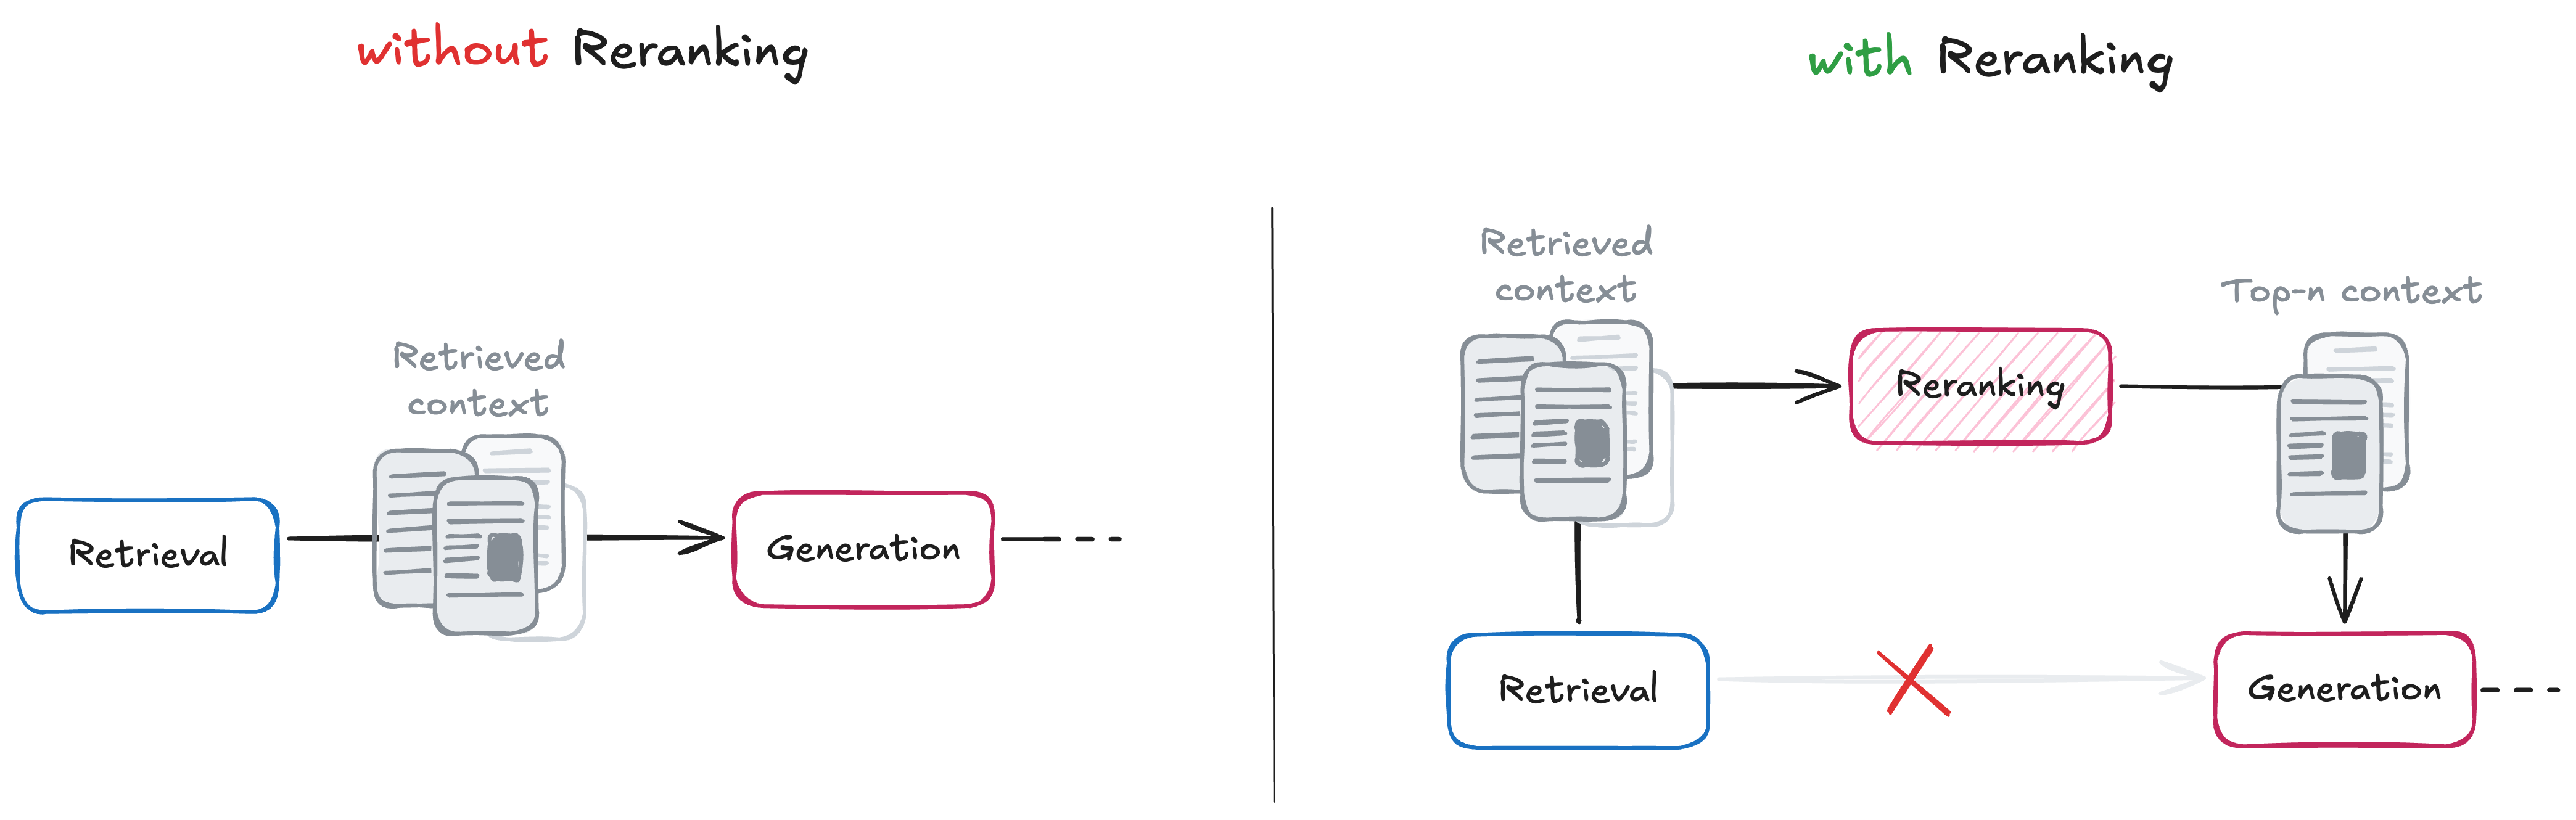
\includegraphics[width=0.9\textwidth]{reranking-comparison.png}
    \caption{Retrieved context with and without reranking}
    \label{fig:reranking}
\end{figure}

\medskip

Each module is an independent binary toggle. Together, the three toggles define
a configuration vector: HyDE (on/off), retrieval mode (dense/hybrid) and reranking
(on/off). This vector controls pipeline intensity per request. All three add computation and
service calls without changing the system's goal: producing an answer grounded in
retrieved context. During baseline experiments, the configuration is fixed for the
entire run and applied uniformly to all queries. Dynamic per-query adaptation is
introduced in Chapter~\ref{sec:controller}.


% ---------------------------------------------------------------------------
\subsection{Baseline Execution}
\label{subsec:baseline-flow}

In the baseline configuration, all optional modules are enabled. Every query follows the same 
fixed pipeline execution path with no conditional logic:

\begin{figure}[h!]
    \centering
        \centering
        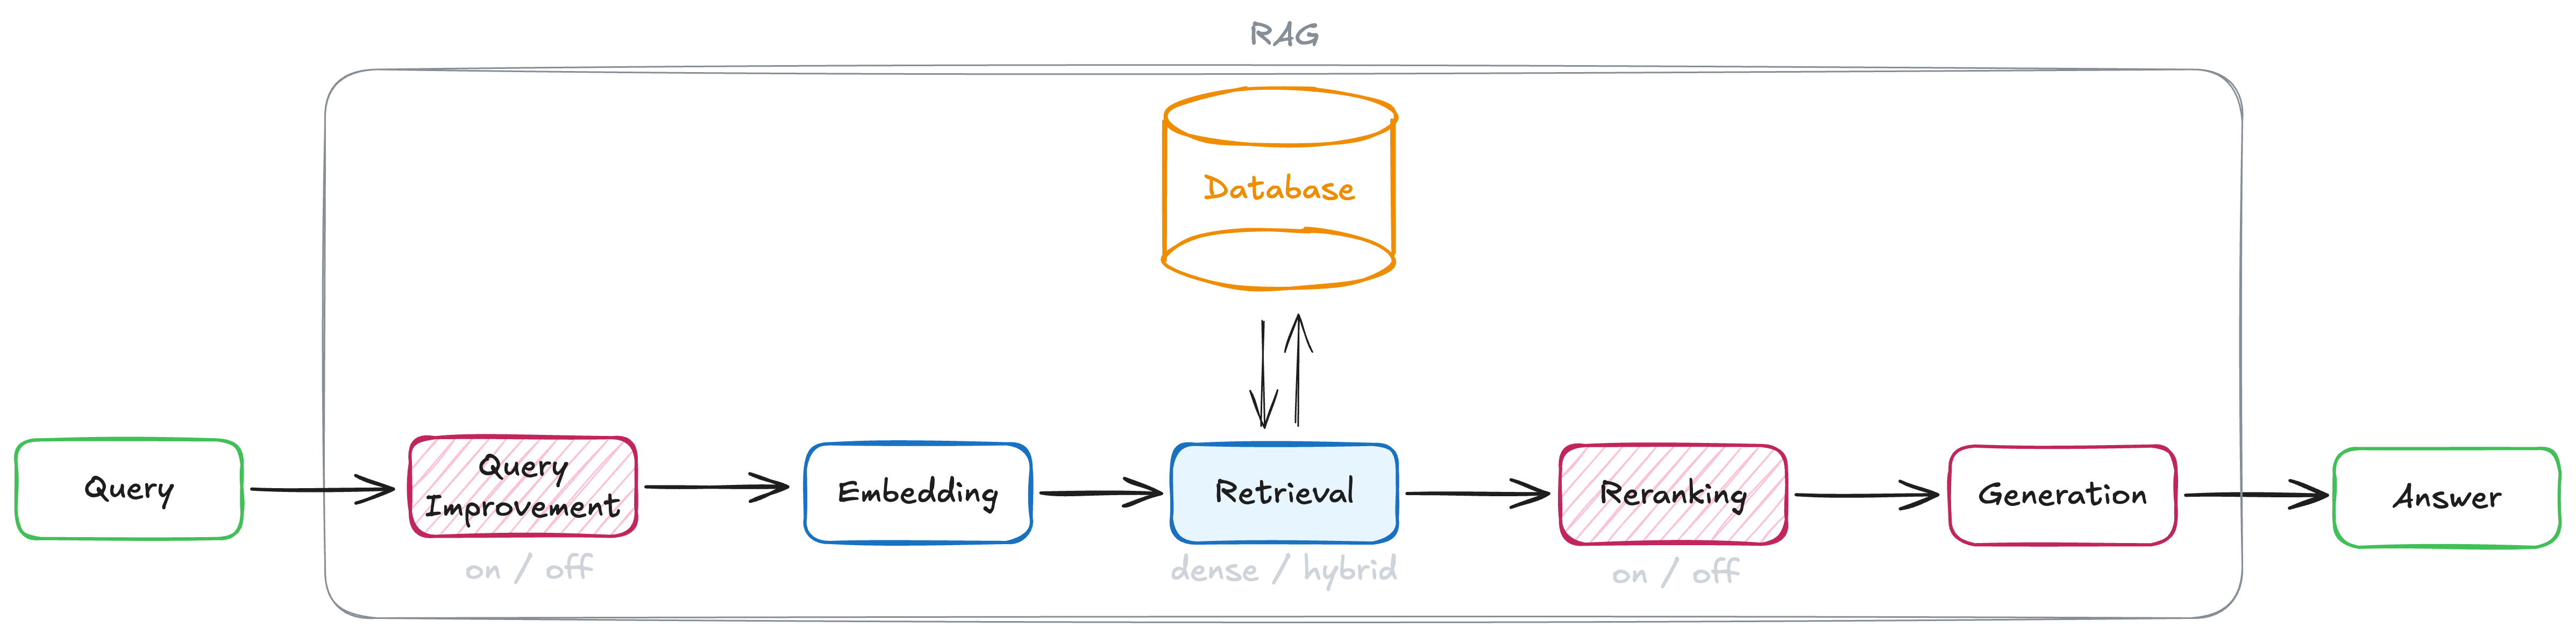
\includegraphics[width=1.0\textwidth]{rag-options.png}
        \caption{RAG Full}
        \label{fig:flow-rag-hyde}
\end{figure}


\begin{enumerate}
    \item \textbf{Query received.} The orchestrator receives the user query.
    \item \textbf{HyDE generation.} The query is sent to the LLM node, which generates a hypothetical answer.
    \item \textbf{Embedding.} The embedding node encodes either the original query or the hypothetical document produced by HyDE.
    \item \textbf{Hybrid retrieval.} The database node performs dense and sparse search, fuses results and returns candidate documents.
    \item \textbf{Reranking.} The embedding node reranks the candidates and selects the top-$n$ passages.
    \item \textbf{Generation.} The LLM node generates the final answer conditioned on the reranked context.
    \item \textbf{Response returned.} The orchestrator returns the answer to the user.
\end{enumerate}

This execution is serial: each stage must complete before the next begins. All queries incur the full computational path regardless of their complexity or characteristics.

% ---------------------------------------------------------------------------
\subsection{Configuration Space}
\label{subsec:baseline-config}
The three optional modules described above: HyDE, reranking and retrieval
type. Each admits two states: on or off (dense or hybrid for retrieval type). 
Combined possibilities listed in Table~\ref{tab:config-space}.

% Combining
% all possibilities yields $2^3 = 8$ configurations, listed in
% Table~\ref{tab:config-space}.

\begin{table}[H]
\centering
\begin{tabular}{lccc}
\hline
\textbf{Config} & \textbf{HyDE} & \textbf{Reranking} & \textbf{Search type} \\
\hline
C0 & off & off & dense   \\
C1 & on  & off & dense   \\
C2 & off & on  & dense   \\
C3 & off & off & hybrid  \\
C4 & on  & on  & dense   \\
C5 & on  & off & hybrid  \\
C6 & off & on  & hybrid  \\
C7 & on  & on  & hybrid  \\
\hline
\end{tabular}
\caption{Configuration space ($2^3$ factorial design).}
\label{tab:config-space}
\end{table}

C0 serves as the minimal baseline: only the core pipeline stages execute. C7 is the
current CITI KMS deployment configuration and serves as the always-on reference against
which energy savings are measured. Single-module configurations (C1, C2, C3) enable
per-module attribution; multi-module configurations (C4--C6) test module interactions.
The following chapter describes the measurement framework used to quantify
the energy and performance characteristics across all eight configurations.

\newpage
\section{Measurement Framework}
\label{sec:method_protocol}


\subsection{Objectives and Scope}
\label{subsec:measurement-objective}


% --- Block A: Measurement Objective ---

The conditional controller proposed in this thesis assumes that optional RAG modules
consume additional energy per request. The CITI KMS system described in
previously has no existing energy benchmarks nor toggled modules. Before designing a
controller, we must first quantify the energy cost of module activation.

To produce this evidence, the measurement framework records estimated energy consumption on each
of the three infrastructure nodes that compose the RAG pipeline:

\begin{figure}[h!]
    \centering
        \centering
        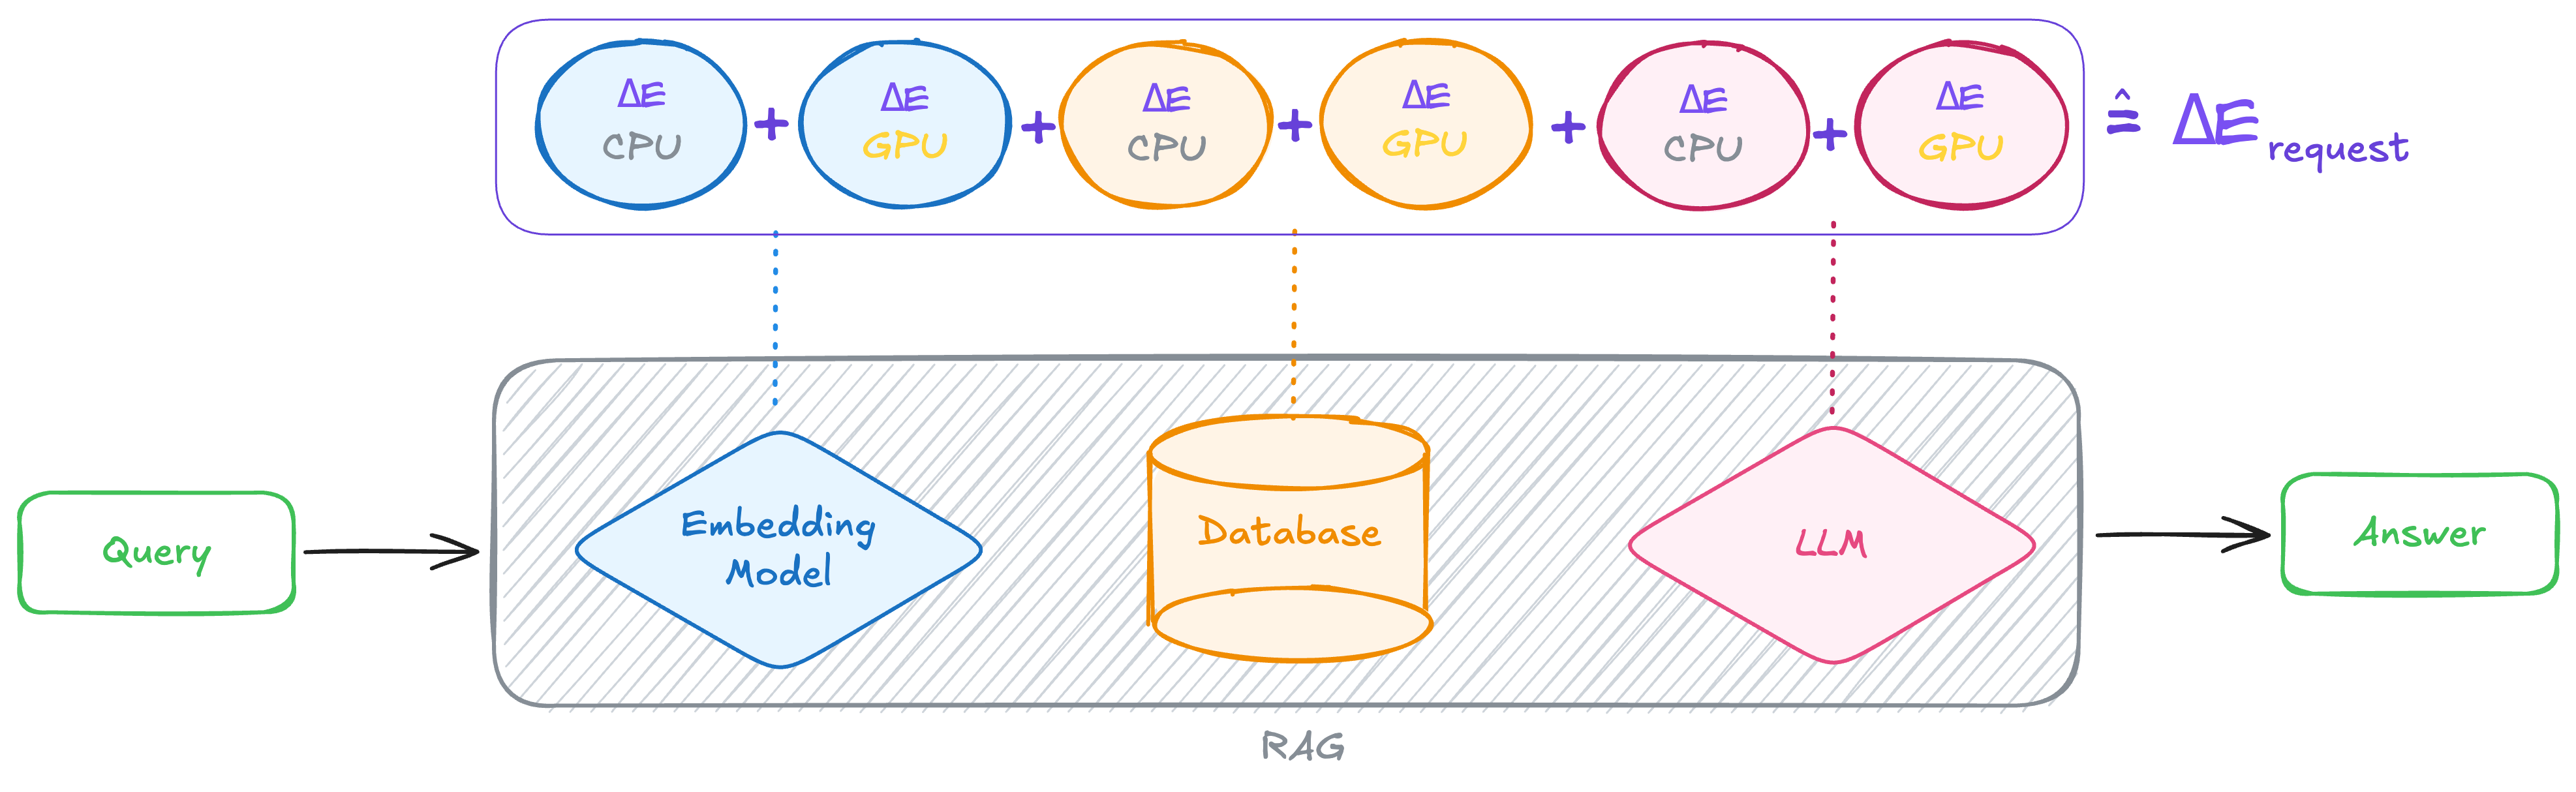
\includegraphics[width=0.8\textwidth]{energy-measurement.png}
        \caption{Node-level energy measurement architecture}
        \label{fig:energy-measurement}
\end{figure}

\begin{itemize}
    \item \textbf{embedding node}, which encodes queries and when reranking is
          active, runs a cross-encoder model;
    \item \textbf{vector-database node} (Milvus), which executes dense or hybrid
          similarity search;
    \item \textbf{LLM node}, which generates the final answer and when
          HyDE is active, produces a hypothetical document.
\end{itemize}

On each node, CPU and GPU energy are read from hardware counters at the start
and end of every request. The reported quantity is total energy per request in
joules, summed across all three nodes.

% writing_note : we need to explain why only CPU and GPU --> if not mentionned in chapter 2
% SOTA that GPU and CPU account for most energy usage

The primary comparison is between C0 (minimal pipeline: all modules off, dense search)
and C7 (the current CITI KMS configuration: all modules on, hybrid search). To enable
finer-grained attribution and provide training data for the controller, we extended the
comparison to all eight possible configurations (C0--C7) defined in
Section~\ref{subsec:baseline-config}. These form a complete $2^3$ factorial design over
three binary module axes: HyDE, reranking, and search type.

\begin{figure}[h!]
    \centering
        \centering
        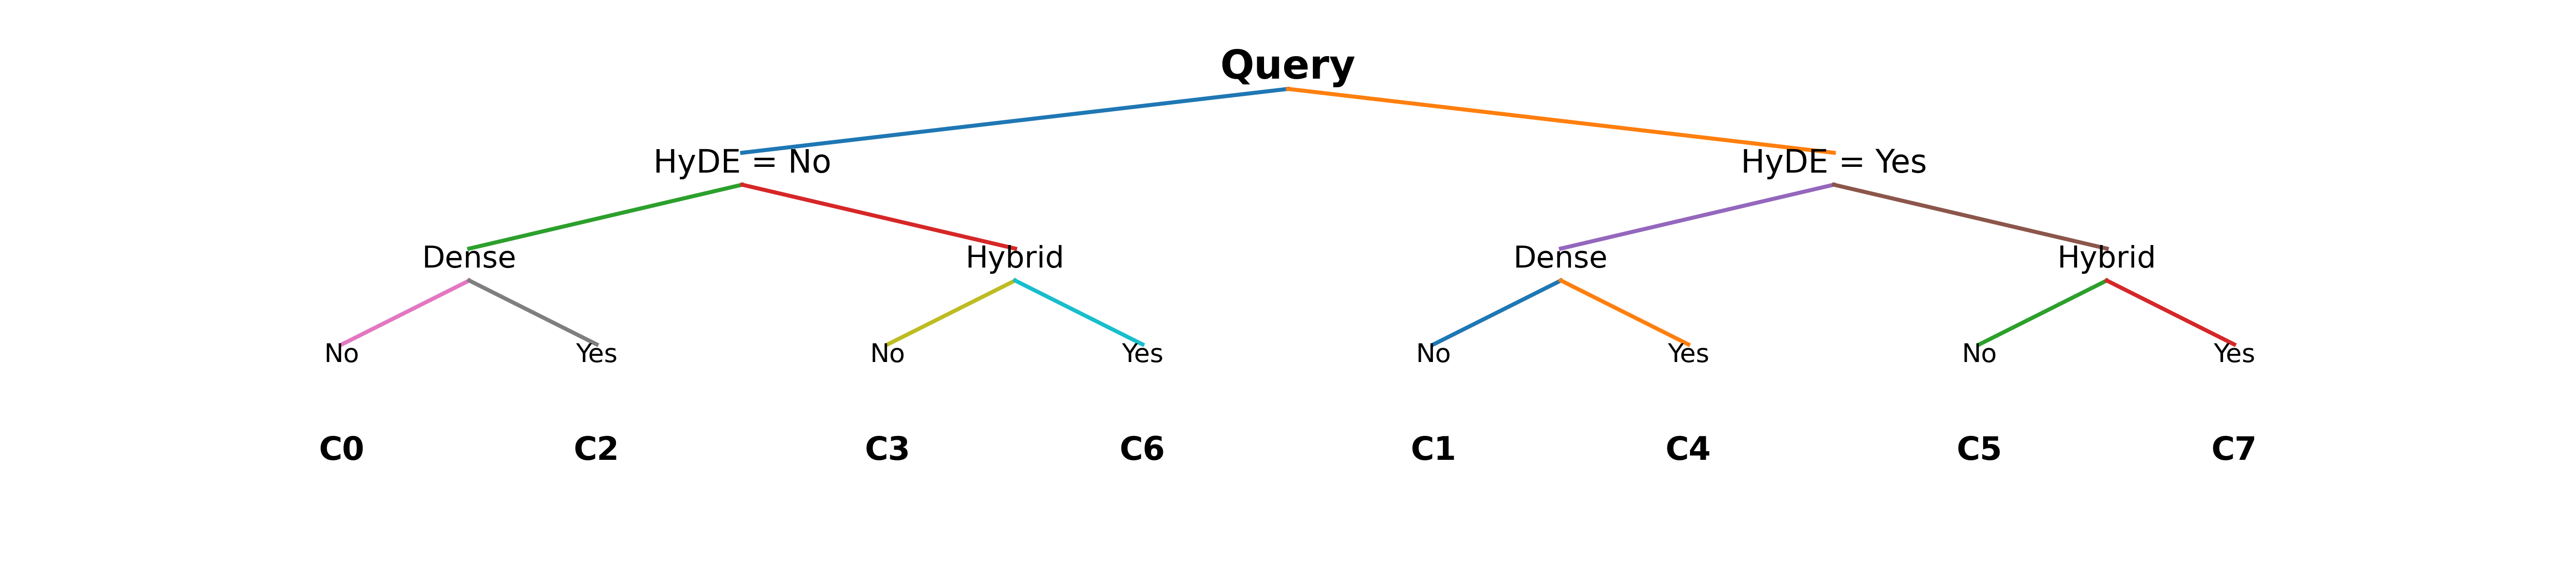
\includegraphics[width=0.8\textwidth]{citi_config_tree_wide.png}
        \caption{$2^3$ factorial configuration space}
        \label{fig:config-tree}
\end{figure}

Energy alone does not suffice to evaluate module activation. A configuration that saves
energy but doubles response time or degrades answer correctness is not useful. Therefore,
each session also records latency and quality metrics.

\subsection{Unit of Analysis}
\label{subsec:unit-of-analysis}

The unit of analysis is a \emph{session}: one query executed under one fixed configuration
until an answer is produced. Every measurement (energy, time to first token, total
time, token counts, quality scores, etc.) is recorded under a unique
\texttt{session\_id}. A session is identified by the tuple \texttt{(query\_id, config\_id)}.

Sessions are executed sequentially with no concurrent load, independently of
configuration order. Each measurement therefore reflects the complete cost of
answering one query under one configuration.

% writing_note : keep this commented - do not delete.
% In total, the experimental dataset comprises 750~queries executed under all
% 8~configurations, yielding 6{'}000~sessions.

In total, each session records approximately 47~fields spanning energy, timing, token
counts, retrieval statistics, and stage-level attribution. Section~\ref{subsec:metrics} 
lists these fields and their definitions.

% % --- Block C: System Boundary ---

Each node runs a lightweight metrics module that reads hardware energy counters
at the start and end of every session. The orchestrator coordinates session
boundaries across all three nodes via a shared \texttt{session\_id}. Attribution
is at the device level (CPU package, GPU device); the framework does not
decompose energy to individual processes or kernels.
% Section~\ref{subsubsec:energy-metrics} defines the counter sources and
% computation method.

Excluded from the measurement boundary are power-at-the-wall measurements, network
fabric energy, storage I/O energy, and orchestrator computation. The orchestrator
performs no heavy computation; its role is control flow and data assembly.


% % --- Block D: Supporting Metrics ---
Beyond energy, each session records latency (time to first token, total
response time), token counts (query, augmentation, context, answer), retrieval
traces (pre-rerank, post-rerank, final context), and quality scores
(deterministic, provenance-based, and LLM-assisted). These supporting
measurements ensure that no energy claim is made without the corresponding
operational and quality context.


\subsection{Metrics Definition}
\label{subsec:metrics}
% This chapter defines what is measured and how. Interpretation belongs to
% Chapter~\ref{sec:baseline_analysis}. Section~\ref{subsec:metrics} specifies each metric's
% unit, computation method, and role in the analysis.

\subsubsection{Energy Metrics}
\label{subsubsec:energy-metrics}
% --- Block A: Primary energy quantities ---
Request energy represents the total device-level cost of answering one query
under one configuration. It is computed as the sum of the three infrastructure
nodes:
$$E_{\text{request}} = E_{\text{emb. model}} + E_{\text{database}} + E_{\text{llm}}$$

Each node contributes CPU and GPU energy:
$$E_{\text{node}} = E_{\text{cpu}} + E_{\text{gpu}}$$

where:
\begin{itemize}
    \item \textbf{$E_{cpu}$} is read from Intel RAPL counters, which report
          cumulative energy in microjoules ($\mu$J), converted to joules (J).
    \item \textbf{$E_{gpu}$} is read from the NVIDIA NVML interface, which
          reports cumulative energy in millijoules (mJ), converted to joules (J).
\end{itemize}

Both counter types are monotonic. Session energy is computed as a counter delta:
$\Delta E = E_{\text{end}} - E_{\text{start}}$ within the session window.

Energy is reported in joules rather than watts. Watts measure instantaneous
power draw; joules capture total energy consumed over the session window, which
matches the per-request comparison objective.

% --- Block B: Normalization (J/token) ---
In LLM systems, computation cost scales approximately with the number of tokens
processed. Because configurations change token counts per request, HyDE adds
augmentation tokens, reranking alters context length; normalizing energy by
total tokens controls for workload-size differences:

% writing_notes :
% allows comparison across: batch sizes, contexts, generation lengths, datasets
% Energy per token approximates:
% FLOPs per token × Energy per FLOP

$$E_{\text{token}} = \frac{E_{\text{request}}}{N_{\text{total\_tokens}}} \quad [\text{J/token}]$$

Joules per token serves as a comparison aid when output lengths differ across
configurations. It is not a perfect universal efficiency metric. It still ignores retrieval
cost amortization, query-level fixed energy overhead and short-answer bias but takes 


\subsubsection{Latency Metrics}
\label{subsubsec:performance-metrics}

% --- Block D: Latency ---
Two main latency measures capture the operational cost of each session:

\begin{figure}[h!]
    \centering
        \centering
        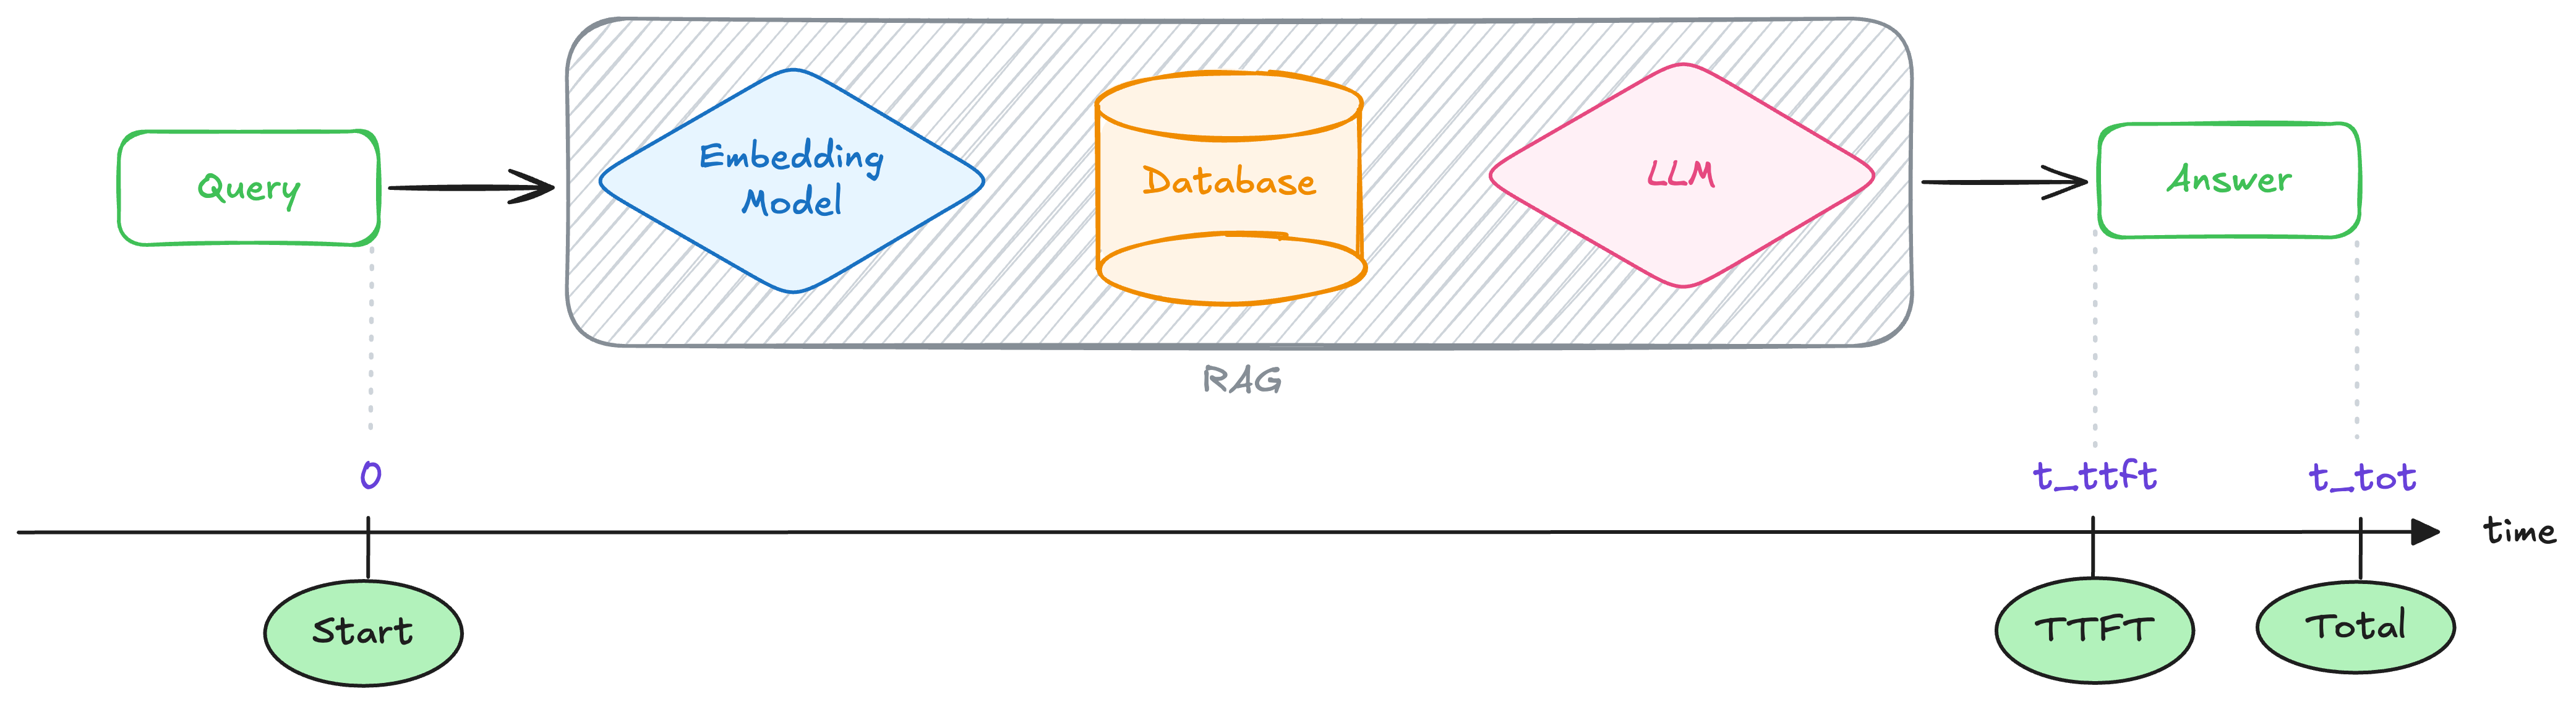
\includegraphics[width=0.8\textwidth]{latency.png}
        \caption{Latency measurement points}
        \label{fig:latency-measurement}
\end{figure}

\begin{itemize}
    \item \textbf{Time to first token (TTFT)} elapsed time in milliseconds
          from query submission to the first generated token. TTFT reflects
          user-perceived responsiveness and is sensitive to pre-generation stages
          such as HyDE and reranking.
    \item \textbf{Total response time} elapsed time in milliseconds from
          query submission to answer completion. This measures end-to-end duration.
\end{itemize}

Their difference can be defined as generation time. Per-stage timing intervals (embedding, 
retrieval, reranking, HyDE, generation)
are also recorded. They connect module activation to latency contributions and
support energy attribution by stage. 

% --- Block E: Token accounting ---

Each session records five token counts that describe workload size:
\begin{itemize}
    \item \textbf{query\_tokens}: tokens in the original user query
    \item \textbf{augm\_tokens}: tokens produced by HyDE (zero when HyDE
          disabled)
    \item \textbf{context\_tokens}: tokens in the retrieved context assembled
          for the LLM
    \item \textbf{answer\_tokens}: tokens in the generated answer
    \item \textbf{total\_tokens}: sum of the above four fields
\end{itemize}

Token counts serve two roles. First, they characterize how each configuration
changes workload composition (HyDE adds augmentation tokens; 
context length altered by reranking). 
Second, total tokens provides the denominator for energy
normalization (J/token) as defined earlier.


\subsubsection{Quality Proxies}
\label{subsubsec:quality-proxies}

The studied configurations activate modules that primarily affect retrieval
and context selection. Quality evaluation must therefore cover answer
correctness, retrieval correctness and grounding faithfulness.
No human evaluation is performed; all scores are computed by deterministic
text comparisons or LLM-assisted metrics and treated as proxies, not as
ground truth.

% --- HotpotQA benchmark metrics ---

\paragraph{HotpotQA benchmark metrics}~\cite{hotpotqa2018} provide
deterministic, reproducible scoring across the three evaluation axes:

\begin{itemize}
    \item \textbf{Answer~F1} token-level overlap between the generated
          answer and the reference answer after normalization (lowercasing,
          article and punctuation removal). Exact Match~(EM) is the
          corresponding binary variant.
    \item \textbf{Supporting Facts~F1} paragraph-level retrieval
          correctness: measures whether the pipeline retrieved the gold
          supporting-fact paragraphs annotated in the dataset.
    \item \textbf{Joint~F1} product of Answer~F1 and Supporting Facts~F1;
          rewards correct answers only when supported by correct retrieval.
\end{itemize}

Joint~F1 separates two failure modes: ``answer looks right but retrieval
failed'' versus ``answer is supported by the correct documents.'' This
distinction matters because the studied modules (HyDE, reranking, hybrid
search) primarily affect retrieval behavior.

% --- LLM-assisted quality (RAGAS) ---

\paragraph{LLM-assisted metrics} add semantic evaluation that string-based
metrics miss. The LLM-as-judge paradigm uses a language model to score
generated answers against references or contexts;
vRAG-Eval~\cite{vrageval2024} reports 82.6\% agreement between GPT-4
judgments and human annotations on RAG evaluation tasks. The thesis uses the
RAGAS framework~\cite{ragas2023} with two primary metrics, scored 0~to~1:

\begin{itemize}
    \item \textbf{Faithfulness} fraction of claims in the generated
          answer that are supported by the retrieved contexts.
    \item \textbf{Factual correctness} semantic agreement between
          the generated answer and the reference answer.
\end{itemize}

Faithfulness detects hallucination (unsupported claims); factual correctness
detects wrong answers (semantic mismatch with the reference). Together with
Answer~F1, they form the quality basis for the acceptability thresholds
defined in Chapter~\ref{sec:controller}. A dedicated evaluator model
(Qwen2.5-14B-Instruct), distinct from the pipeline LLM, scores
each answer; results are treated as assisted evaluation, not as
oracle truth.
% and scores should be interpreted comparatively across configurations (DO NOT DLT - keep commented)
% rather than as absolute quality measures. (DO NOT DLT - keep commented)


\subsection{Benchmark Dataset}
\label{subsec:dataset}
The measurement framework requires three aligned artifacts: 
a reference answer, gold supporting-fact annotations, and a retrieval corpus. 
This thesis utilizes HotpotQA~\cite{hotpotqa2018}, a multi-hop 
benchmark requiring information synthesis across multiple documents.

HotpotQA was selected for three primary reasons. First, its multi-hop 
structure mimics high-level knowledge management behavior, where users 
often seek to synthesize information across disparate internal sources. 
Second, the dataset is well-documented in existing literature with clear, 
comparable benchmarks, providing a rigorous baseline for our system's 
quality evaluation. Finally, multi-hop queries exercise the full RAG pipeline: 
retrieval must surface multiple documents and generation must synthesize across 
them. This complexity is a prerequisite for routing research, as it should create 
variation in module utility—some queries require advanced modules like 
reranking to succeed, while others do not.

While other knowledge-intensive datasets were considered, HotpotQA provided 
a better balance of reasoning depth and benchmarking clarity.

\begin{figure}[h!]
    \centering
    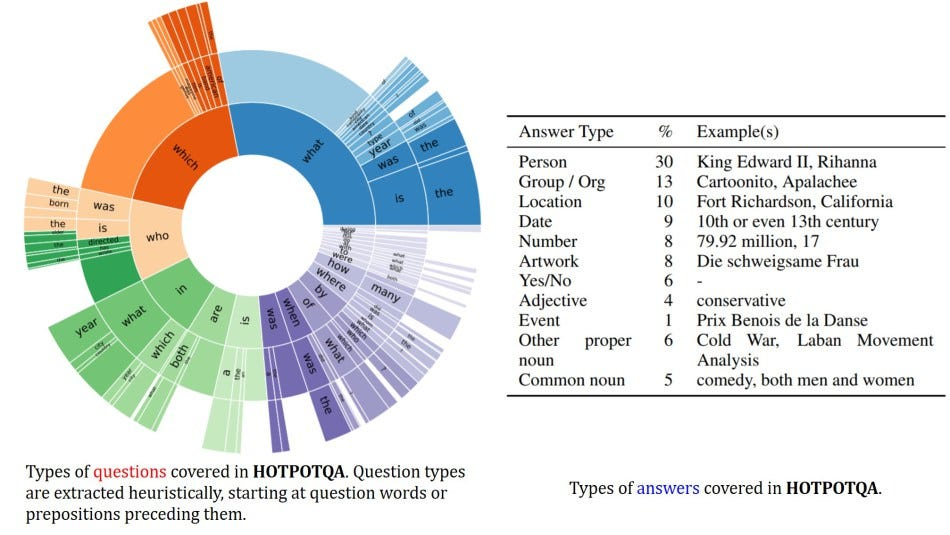
\includegraphics[width=0.85\textwidth]{hotpot.jpg}
    \caption{HotpotQA question and answer type distributions~\cite{hotpotqa2018}}
    \label{fig:hotpot}
\end{figure}

The full HotpotQA distractor split contains approximately 7,400 queries. 
However, executing each query under all eight configurations yields 59,200 
total sessions. To manage the computational demand and time constraints 
associated with running these sessions—specifically the high energy cost of 
LLM-assisted evaluation, we utilized a representative sample of 1,200 queries; 
Split equally between 600 bridge queries (requiring information 
from linked documents) and 600 comparison queries (comparing two entities). 
Each record contains the question text, a reference answer and gold 
supporting-fact paragraphs.

The document corpus consists of the specific Wikipedia pages referenced as 
gold supporting facts for these queries, which were chunked and pre-indexed in 
Milvus. This closed-corpus design ensures that every gold document is present 
in the retrieval index, allowing the Supporting Facts F1 metric to measure 
retrieval effectiveness directly rather than corpus coverage. The implications 
of this reduced retrieval difficulty on domain generalization are further addressed.

\subsection{Experimental Protocol}
\label{subsec:protocol}

% --- Block A: Protocol objective ---

Energy and latency measurements are sensitive to transient system state:
background load, thermal conditions, and caching effects can introduce
variation unrelated to configuration differences. The experimental protocol
controls for these factors by enforcing a fixed workload, a fixed
configuration per session, and deterministic scheduling. The same protocol is
reused when evaluating the controller in Chapter~\ref{sec:strategies}, so that
energy deltas between baseline and controlled execution remain comparable.

% --- Block B: Configuration space ---

The configuration space is the $2^3$ factorial design introduced in
Section~\ref{subsec:baseline-config}: three binary module axes (HyDE,
reranking, search type) yield eight configurations (C0--C7). Each
configuration is fixed for the duration of a session; there is no mid-request
switching. Table~\ref{tab:configs} lists all eight configurations with their
module settings.

\begin{table}[h!]
\centering
\begin{tabular}{c c c l l}
\hline
\textbf{Config} & \textbf{HyDE} & \textbf{Reranking} & \textbf{Search type} & \textbf{Description} \\
\hline
C0 & off & off & dense  & minimal pipeline \\
C1 & on  & off & dense  & + HyDE  \\
C2 & off & on  & dense  & + reranking \\
C3 & off & off & hybrid & + hybrid \\
C4 & on  & on  & dense  & + HyDE + reranking \\
C5 & on  & off & hybrid & + HyDE + hybrid \\
C6 & off & on  & hybrid & + reranking + hybrid \\
C7 & on  & on  & hybrid & all modules \\
\hline
\end{tabular}
\caption{Configuration space: $2^3$ factorial over three binary module axes.}
\label{tab:configs}
\end{table}

% --- Block C: Experimental unit and dataset size ---

The full experiment runs all 1{'}200~queries through all
8~configurations, producing 9{'}600~sessions. Each session logs raw energy
traces, timing metadata, token counts, retrieval traces and the generated
answer text. Runs order are shuffled to reduce systematic drift effects.
Post-hoc evaluation scripts then compute deterministic quality
metrics (Answer~F1, Supporting Facts~F1, Joint~F1) and LLM-assisted metrics
(RAGAS faithfulness, factual correctness) from the stored artifacts.

This dataset serves three purposes: benchmarking the CITI KMS system for
the first time against literature baselines, the baseline trade-off analysis
in Chapter~\ref{sec:baseline_analysis} and generate the training data for the
conditional controller in Chapters~\ref{sec:controller}--\ref{sec:strategies}.

% --- Block D: Execution scheduling ---

A checkpoint file records every completed session. If a run is interrupted, it
resumes from the last checkpoint without re-executing completed sessions. Failed
sessions are logged and excluded; they do not silently corrupt the dataset.

% --- Block E: Session procedure ---

Each session follows a fixed procedure:

\begin{enumerate}
    \item The orchestrator creates a unique \texttt{session\_id} and records the
          query identifier, configuration identifier and run number.
    \item The orchestrator broadcasts a \texttt{start} signal to all three
          infrastructure nodes. Each node begins reading energy counters and
          opens a session buffer.
    \item The pipeline executes the request under the fixed configuration:
          embedding, retrieval (dense or hybrid), optional HyDE, optional
          reranking, context assembly and generation.
    \item Stage marks (start and end timestamps) are emitted for each major
          pipeline stage. Marks are best-effort; a missed mark does not abort
          the session.
    \item After the answer is produced, the orchestrator broadcasts a
          \texttt{stop} signal. Each node closes its buffer and returns the
          collected traces.
    \item All artifacts: energy traces, session metadata, retrieval trace,
          answer text and stage intervals are persisted under the \texttt{session\_id}.
\end{enumerate}

Session energy is computed as a counter delta over the start-to-stop window.
% The framework does not subtract an idle baseline; because all configurations
% run under the same protocol, energy deltas between configurations remain
% meaningful without idle subtraction.

% --- Block F: Post-hoc evaluation ---

Evaluation is separated from execution. Deterministic metrics (Answer~F1,
Supporting Facts~F1, Joint~F1) are computed offline from the stored answer
texts and retrieval traces. RAGAS metrics (faithfulness, factual correctness)
are computed by a separate evaluation script that retrieves context documents
from Milvus and invokes a dedicated evaluator model (Qwen2.5-14B-Instruct),
distinct from the pipeline LLM to avoid self-evaluation bias and a perfomance ceiling. 

This separation keeps the online request path simple and allows the analysis to
be rerun. For example, with updated frameworks, metrics or corrected provenance
mappings, without re-executing all the sessions.

% Evaluation is separated from execution. Deterministic metrics (Answer~F1,
% Supporting Facts~F1, Joint~F1) are computed offline from the stored answer
% texts and retrieval traces. RAGAS metrics (faithfulness, factual correctness)
% are computed by a separate evaluation script that retrieves context documents
% from Milvus.

% This separation keeps the online request path simple and allows the analysis to
% be rerun. For example, with updated frameworks, metrics or corrected provenance
% mappings, without re-executing all the sessions.

% Also it invokes a dedicated evaluator model (Qwen2.5-14B-Instruct),
% distinct from the pipeline LLM to avoid self-evaluation bias.
% Recent benchmarks show that evaluator reliability scales with model size and
% that instruction-tuned models produce more consistent judgments on open-ended
% quality metrics~\cite{llmasjudge2024}; we therefore select a 14B instruct model
% as the largest evaluator our infrastructure can serve alongside the pipeline.

% --- Block G: Validity criteria ---

Several validity checks are applied before any session enters the analysis
dataset. Energy counters must be monotonic within a session; a negative delta
invalidates that node's energy for the session. Each session must contain
start and stop boundaries for every node included in the energy total. Sessions
that fail any check are flagged and excluded from the analysis. No silent
corrections are applied; exclusion is preferred over ad-hoc imputation.

% --- Block H: Protocol invariance ---

All experiments in this thesis: baseline analysis controller training
and controller evaluation use the same query set, the same corpus and
index, the same eight configurations, the same measurement boundary and the
same logging artifacts.


\subsection{Features}
\label{subsec:router-features}

% --- Block A: Feature record policy ---

The conditional controller proposed predicts a
configuration \emph{before} the pipeline executes. This constraint divides the
logged data into two categories:

\begin{itemize}
    \item \textbf{Pre-execution features} are derived from the query text alone.
          They include :
          \begin{itemize}
            \item \textbf{surface statistics} character and token counts, sentence count)
            \item \textbf{question-type indicators} question word, definition or list intent, logical operators
            \item \textbf{complexity signals} named-entity count and diversity, noun-phrase count, content-word ratio
            \item \textbf{semantic features} embedding norm, cosine similarities to query-type centroids
          \end{itemize}
          These 23~features are computable before any pipeline stage runs.
    \item \textbf{Post-execution features} are produced by the pipeline and these are available only after the session completes.
    \begin{itemize}
            \item \textbf{retrieval scores } top-1 similarity, score gaps
            \item \textbf{context statistics} context length, number of documents, truncation ratio
            \item \textbf{token counts} 
            \item \textbf{quality metrics} 
      \end{itemize}

\end{itemize}

Pre-execution features serve as router inputs. Post-execution features are
logged for analysis but cannot serve as controller inputs without running
(and paying the cost of) at least part of the pipeline.
Chapter~\ref{sec:controller} formalizes this distinction and defines the
feature groups used for training.

% --- Block B: Feature persistence ---

Feature extraction is performed offline: a dedicated script computes all
23~pre-execution features for the 1{'}200~queries and stores them alongside the
query identifiers. The same session artifacts that feed the baseline analysis
also feed the controller training pipeline. This avoids a second, inconsistent
data-collection step and ensures that the router is trained on the exact system
behavior measured in this chapter.








% % ============================================================================
% DO NOT DELETE  : 
% Factoid queries
% Straightforward, single-hop questions that can typically be answered from one document / one passage.

% Multi-document queries
% Questions that intentionally require retrieving information from multiple documents and combining them (e.g., compare, aggregate, reconcile).

% Reasoning / implication queries
% Queries where the answer requires inference beyond direct lookup, using retrieved facts to draw a conclusion, explain consequences, or propose a next step.

% Ambiguous / underspecified queries
% Real users ask: “How does this work again?” or “What’s the process?”
% These are where HyDE/query expansion often matters.

% Negative / no-answer queries
% Questions that shouldn’t be answered from the corpus (not present, out of scope).
% This is crucial if your controller also decides “don’t retrieve” or “retrieve but abstain”.

% If you add just (2) underspecified and (3) no-answer, your dataset becomes much more “future-proof” for real traffic.

% A sharper way to frame the dataset

% Instead of “3 types of questions”, you can describe it as training coverage across two axes:

% Retrieval breadth: single-doc → multi-doc

% Answer processing: extractive → compositional → inferential

% Your three buckets are basically corners of this grid—good! The improvement is making sure you populate the in-between regions so the classifier doesn’t overfit.

% ---

% We evaluate our retrieval-augmented generation system using the KILT benchmark (Petroni et al., NAACL 2021), which provides a standardized Wikipedia corpus, curated query sets, and gold provenance annotations. This allows rigorous evaluation of both retrieval correctness and answer quality while enabling controlled system-level measurements.
% -->  if we Use KILT as the academic reference Add your own domain corpus (lab documents)
%     You compare: Δ system behavior under identical queries. This is key.
%             “We evaluate our RAG system on KILT, a standardized benchmark for knowledge-intensive NLP tasks grounded in Wikipedia.”

%             You are no longer benchmarking QA performance

% You are benchmarking system behavior under retrieval uncertainty.

% That’s a different but valid scientific claim.

% Aspect	kilt_wikipedia	kilt_corpus
% QA benchmark fidelity	High	Lower
% Retrieval difficulty	Artificially easier	Realistic
% Noise	Low	High
% Router value	Moderate	High
% Energy signal	Muted	Strong
% Systems relevance	Medium	Very high

% With kilt_corpus, your router actually matters more.

% --> “While KILT provides a task-aligned Wikipedia subset, we intentionally use the full KILT corpus to reflect realistic retrieval conditions. Our objective is not to maximize QA benchmark scores, but to study energy–latency–quality trade-offs in retrieval-augmented systems under large-scale retrieval noise.”



% use Kepler (Kubernetes-based Efficient Power Level Exporter) to collect energy consumption data 2601.02522v2.pdf
\newpage
\section{Performance Analysis}
\label{sec:baseline_analysis}

% Chapter purpose: Prove the problem exists.
% Present empirical evidence that always-on module activation is measurably inefficient.
% Three dimensions: energy (5.1), latency (5.2), quality (5.3), then synthesis (5.4).
% Figures source: src/lkc-llm/scripts/experiments/hotpot/2-performance/output/plots/
%                 src/lkc-llm/scripts/experiments/hotpot/3-quality/output/plots/


\subsection{Energy Breakdown}
\label{subsec:energy-breakdown}

% --- Experimental anchor ---

Earlier, we introduced the hypothesis that the optional RAG stages
require more energy, implying that not all of the options need to be active for
every query to produce acceptable answers. To test this claim, we executed all
1{'}200~queries under each of the eight configurations, producing
9{'}600~sessions under the protocol defined earlier.
This section presents the energy dimension of
that experiment. The main comparison is between C0 (minimal pipeline) and C7
(all options enabled); single-module configurations (C1, C2, C3) isolate
per-modules contributions. Table~\ref{tab:configs} lists all eight
configurations and their module settings.

% --- Total energy per request and Energy/token

The figure below reports the mean total energy per request across
all eight configurations. The baseline consumes 318~J per request on average, while the
KMS pipeline consumes 1{'}786~J---a ratio of 5.6$\times$.

Energy is measured as counter deltas over session windows without subtracting
idle baseline power. During HyDE's additional 4.3\,s, the embedding and
database nodes accumulate an estimated $\sim$70\,J of idle draw---approximately
5\% of HyDE's 1{'}355\,J marginal cost. The qualitative finding is unchanged.
\begin{figure}[h!]
    \centering
    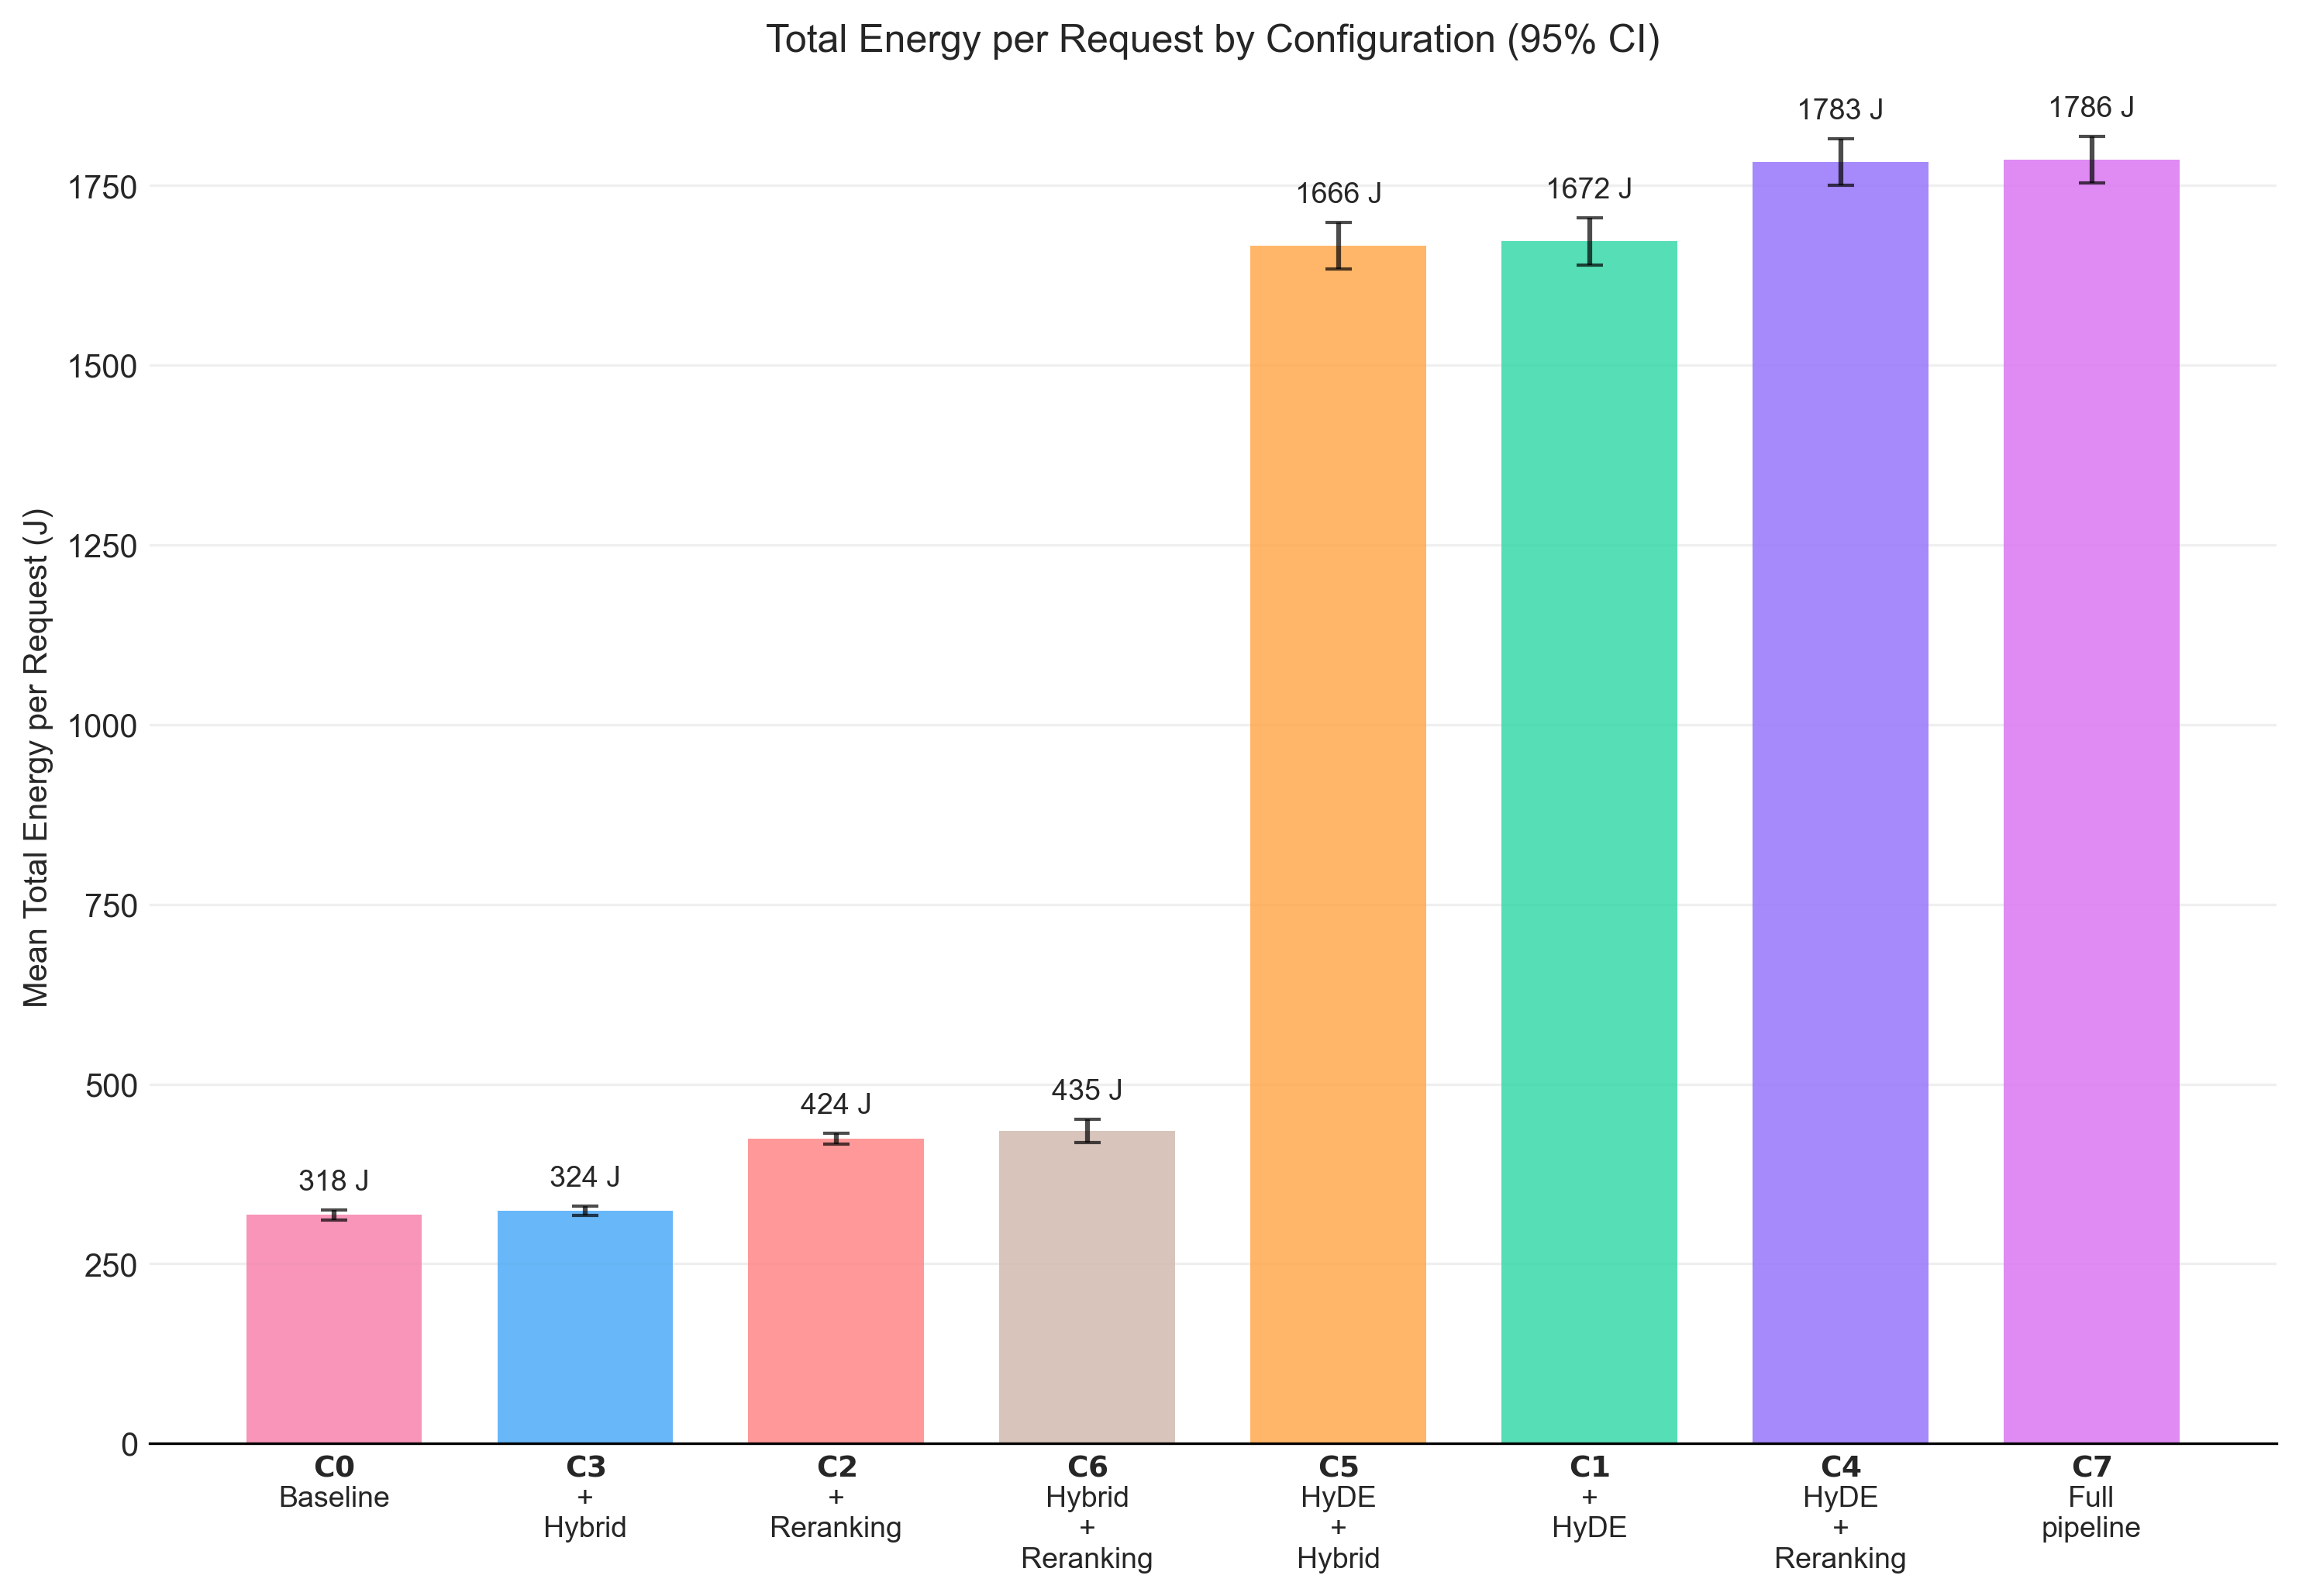
\includegraphics[width=0.85\textwidth]{total_energy_by_config.png}
    \caption{Mean total energy per request across configurations}
    \label{fig:total-energy}
    % Source: hotpot/2-performance/output/plots/total_energy_by_config.png
\end{figure}

Two energy clusters emerge:
\begin{itemize}
    \item Configurations that include HyDE (C1, C4, C5, C7) form a high-energy group 
    between 1{'}666--1{'}786~J.
    \item Configurations not including HyDE which cluster below 435~J, with hybrid retrieval (C3)
    nearly identical to C0 (324~J against 318~J), adding only 2\% energy overhead.
\end{itemize}

Module costs are approximately additive given the hybrid search influence.
C7 (1{'}786~J) exceeds C4 (1{'}783~J) by only 3~J, closely matching the 6~J cost of hybrid retrieval
alone (C3$-$C0). Given that, the per-module analysis in the next section characterises
each module's energy overhead, focusing on the cross-module comparisons.

% --- Stage-level energy attribution ---

Table~\ref{tab:stage-energy} details the five measured stages for C0 and C7.
The prompt augmentation stage (HyDE) is the largest single contributor in the
full pipeline, consuming 1{'}271~J---4.0$\times$ the entire baseline (C0)
request. Reranking adds 111~J. Answer generation remains roughly constant
across configurations (268--302~J), indicating that the LLM generation phase
does not vary with retrieval enrichment.

\begin{table}[h!]
\centering
\begin{tabular}{l r r}
\hline
\textbf{Pipeline stage} & \textbf{Baseline (J)} & \textbf{KMS Pipeline (J)} \\
\hline
Embedding           &  43.2 &   63.6 \\
HyDE (prompt aug.)  &   --- & 1354.5 \\
Retrieval (DB)      &   7.0 &   38.1 \\
Reranking           &   --- &  105.8 \\
Generation          & 267.7 &  302.4 \\
\hline
\end{tabular}
\caption{Stage-level energy attribution (C0 vs C7).}
\label{tab:stage-energy}
\end{table}

% --- Feature attribution ---

The differential view $\Delta E = E(\text{C}_i) - E(\text{C0})$ quantifies
each module's mean marginal cost (Figure~\ref{fig:feature-attribution}). HyDE adds
1{'}355~J per request, reranking adds 106~J and hybrid adds 6~J. HyDE's
marginal cost exceeds the total energy of C0 by a factor of 4.3. The three
modules differ by two orders of magnitude in energy cost.

\begin{figure}[h!]
    \centering
    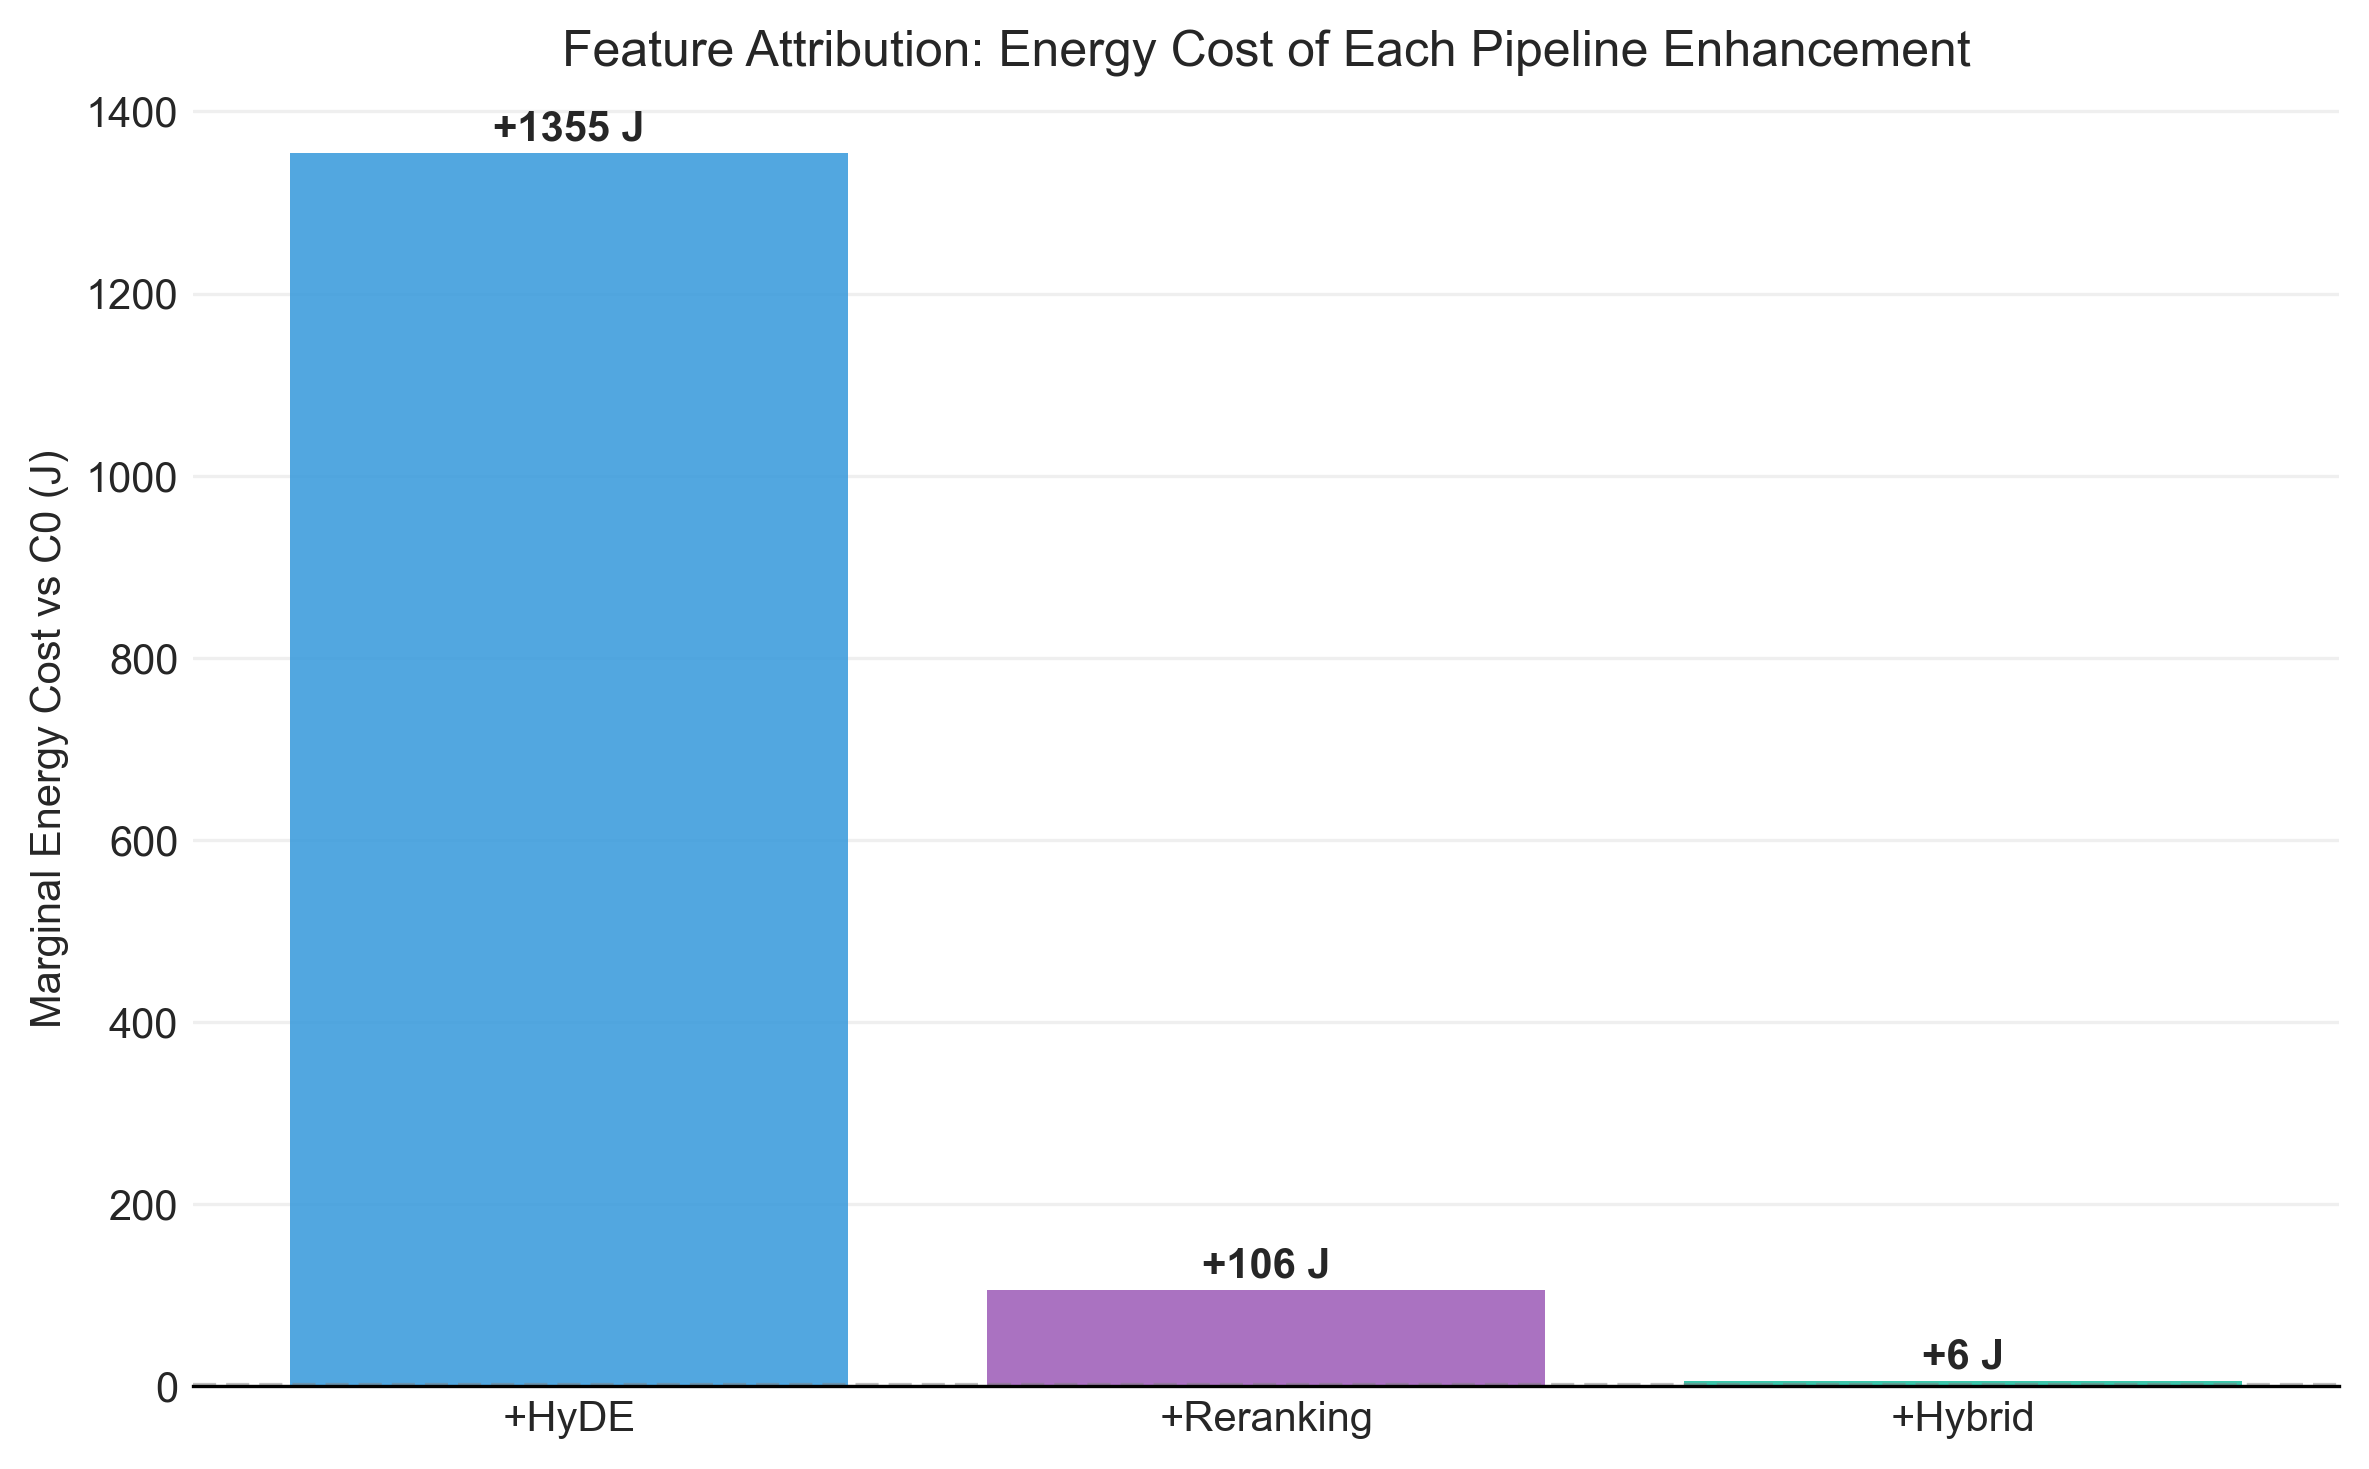
\includegraphics[width=0.85\textwidth]{feature_attribution_energy.png}
    \caption{Marginal energy cost of each module (delta from C0).}
    \label{fig:feature-attribution}
    % Source: hotpot/2-performance/output/plots/feature_attribution_energy.png
\end{figure}

% --- Energy per token ---

Normalizing by total token count yields energy per token (J/tok), which
controls for additional tokens and enables fairer comparison across setups.
C0 consumes 0.39~J/tok while C7 consumes 1.44~J/tok---a 3.7$\times$ ratio,
compressed from the 5.6$\times$ total energy ratio. HyDE generates
additional tokens and remains the most expensive after normalization, 
confirming that the overhead is structural
(an additional LLM call) rather than a token count artifact.

\begin{figure}[h!]
    \centering
    \begin{subfigure}[t]{0.48\textwidth}
        \centering
        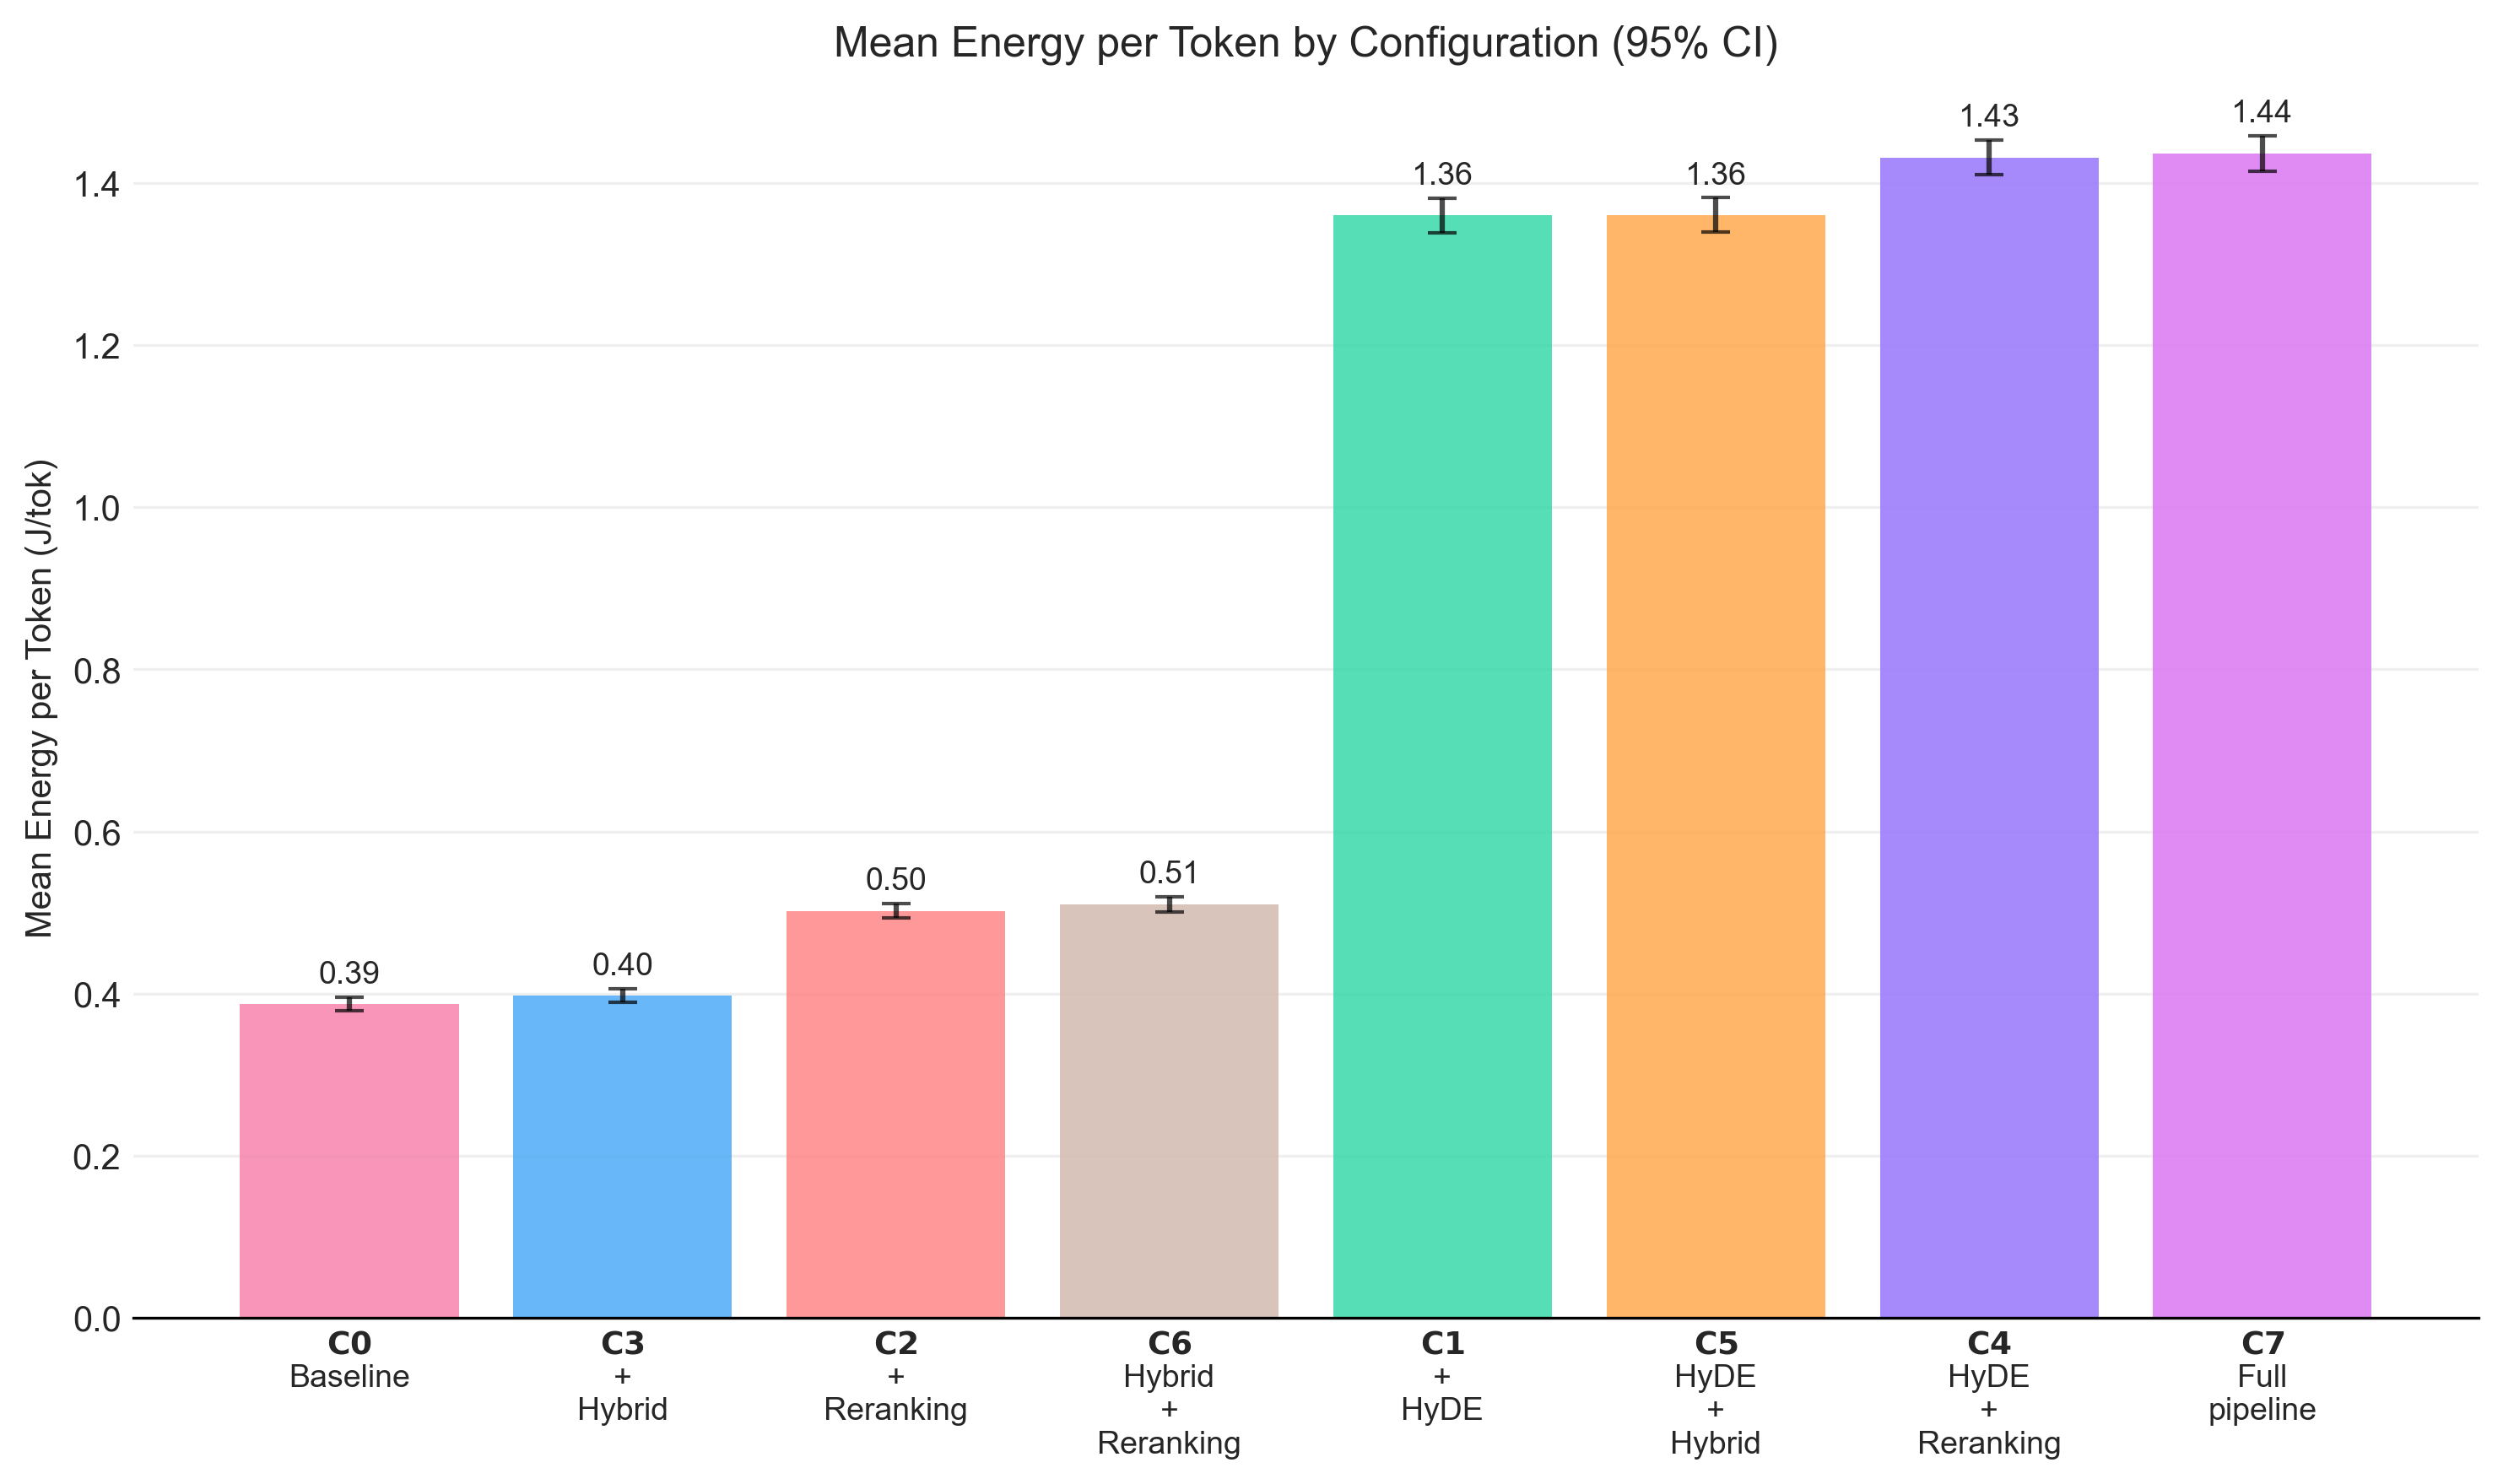
\includegraphics[width=\textwidth]{mean_energy_per_token.png}
        \caption{Mean energy per token}
        \label{fig:energy-per-token-bar}
        % Source: hotpot/2-performance/output/plots/mean_energy_per_token.png
    \end{subfigure}%
    \hfill
    \begin{subfigure}[t]{0.48\textwidth}
        \centering
        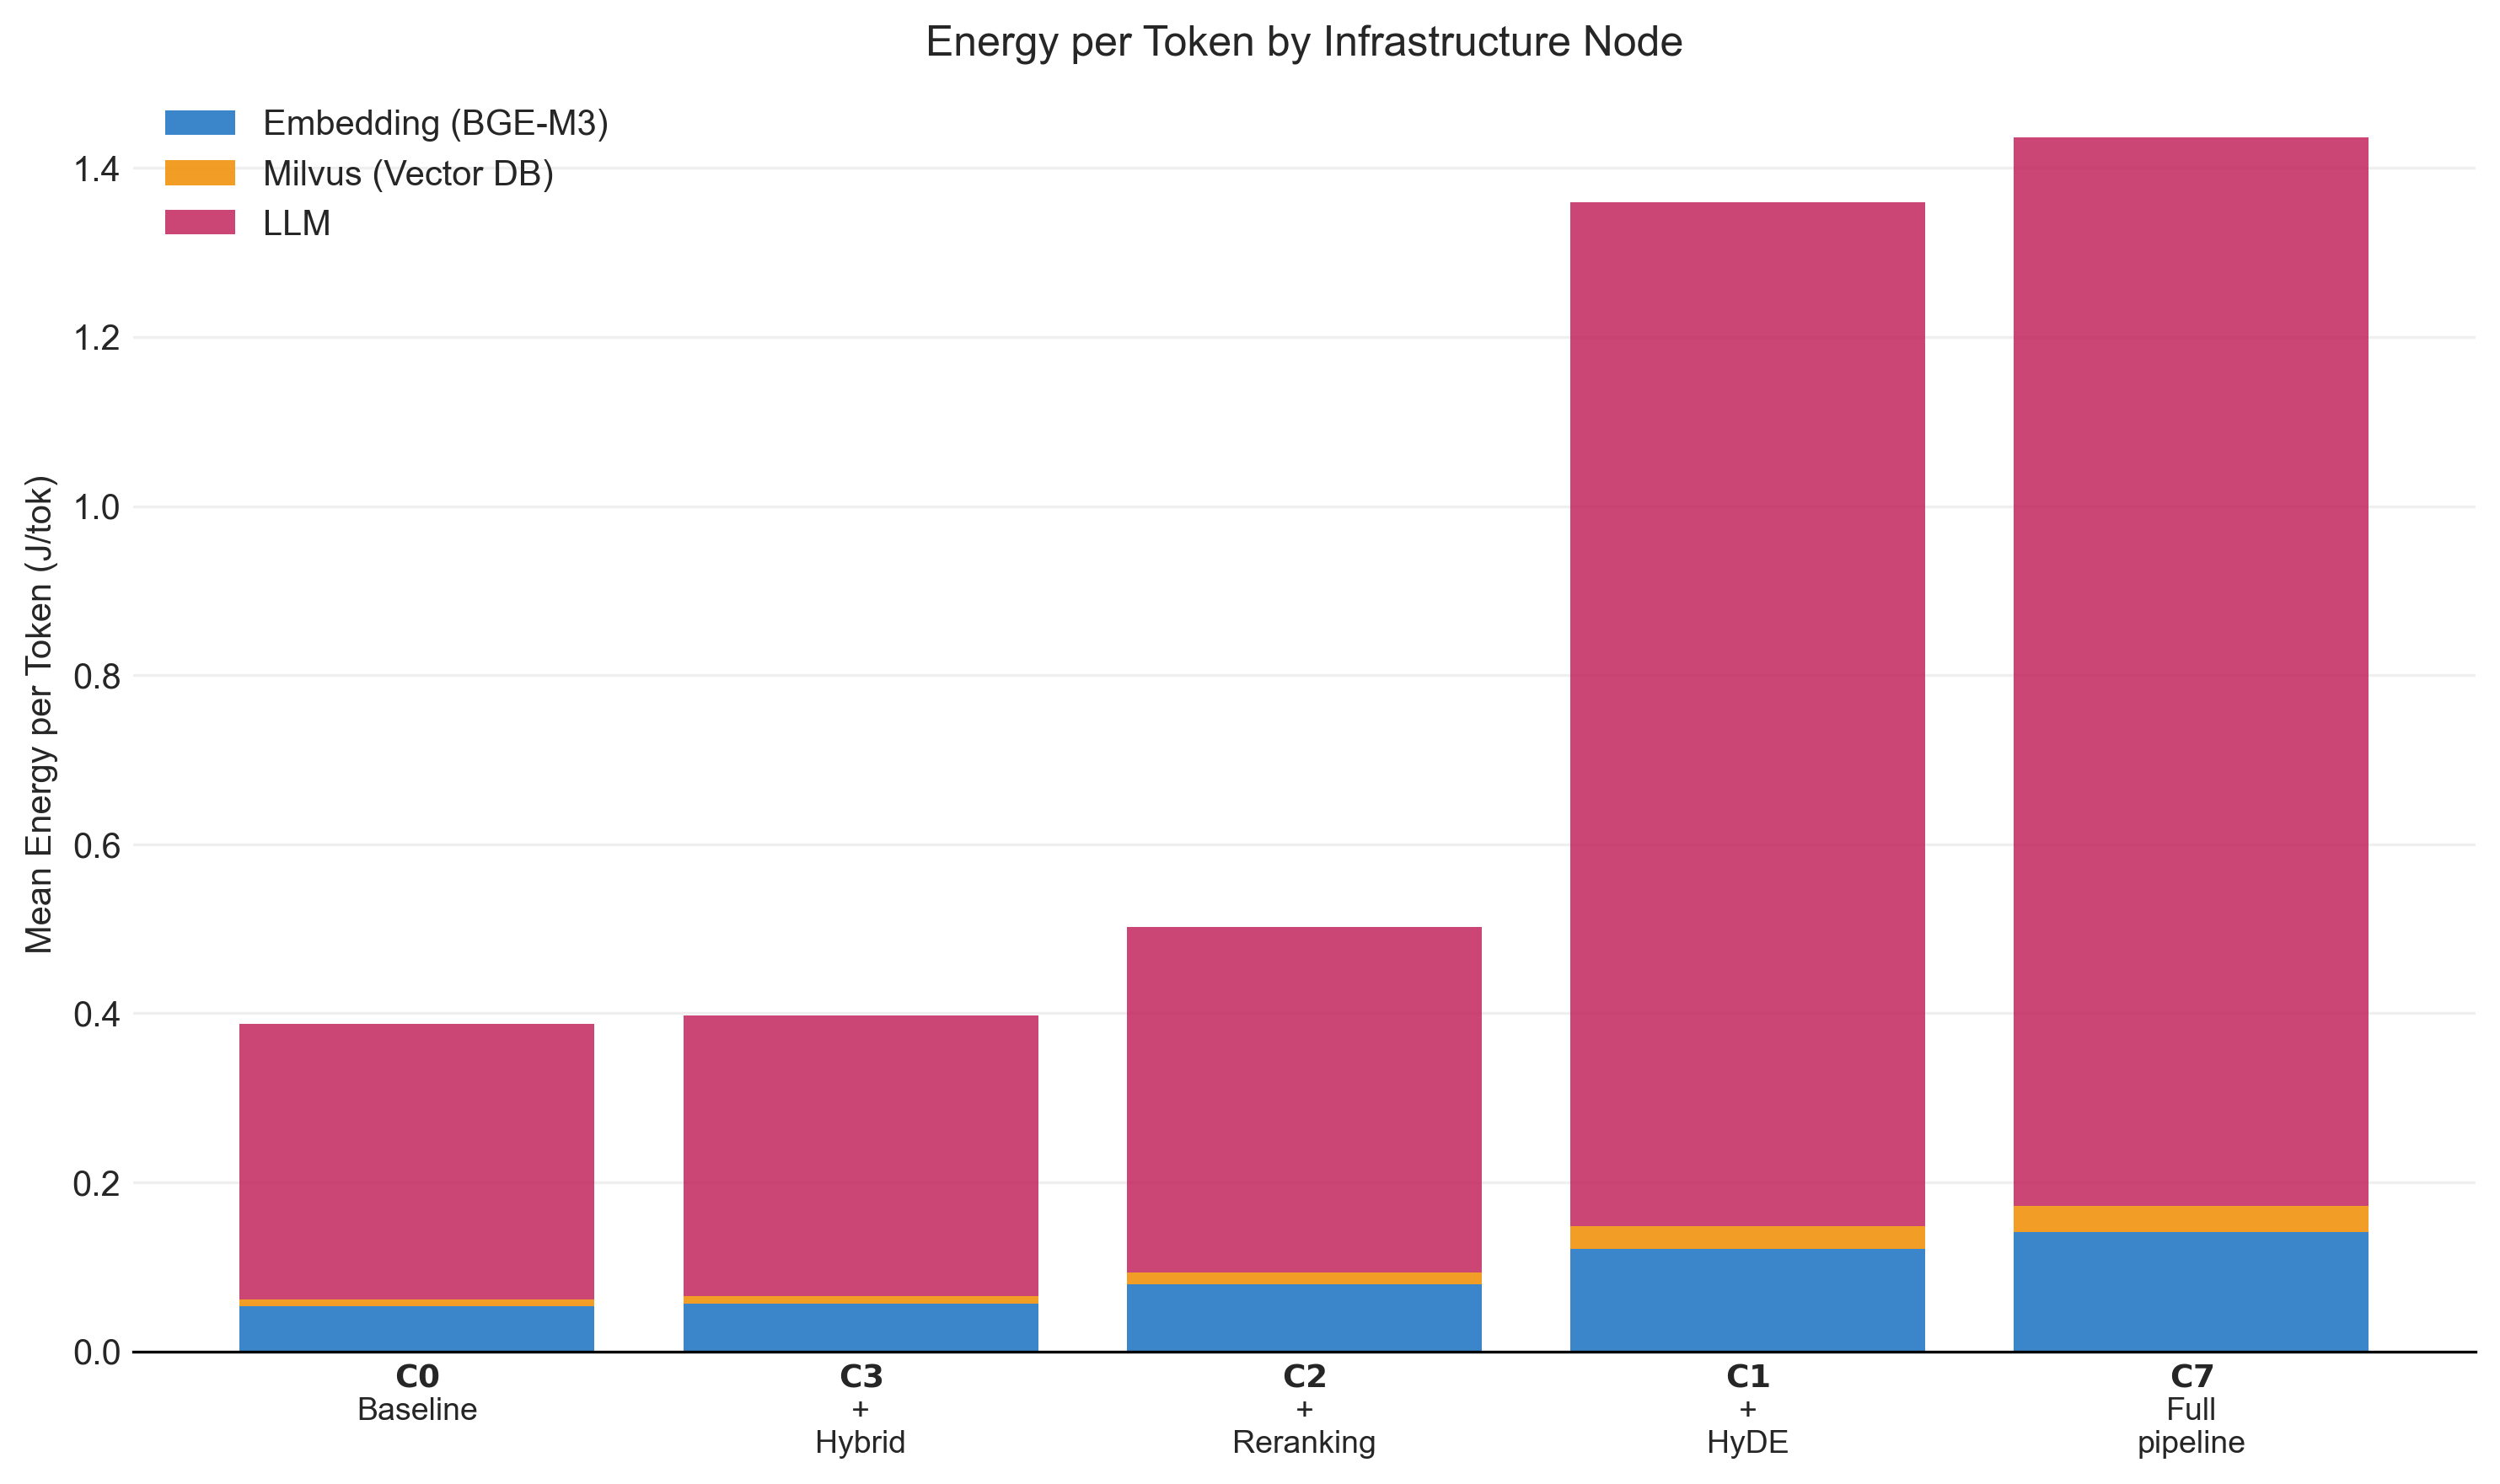
\includegraphics[width=\textwidth]{node_energy_per_token_decomposition.png}
        \caption{Energy per token by infrastructure node}
        \label{fig:node-decomposition}
        % Source: hotpot/2-performance/output/plots/node_energy_per_token_decomposition.png
    \end{subfigure}
    \caption{Energy per token by configuration}
    \label{fig:energy-per-token-combined}
\end{figure}

% --- Node-level decomposition prose ---

Figure~\ref{fig:node-decomposition} decomposes energy per token into the three
infrastructure nodes. The LLM node dominates across all configurations; HyDE
(C1) amplifies LLM node cost through an additional generation pass. The
embedding node contributes a smaller fraction and the Milvus node is negligible.\\


HyDE amplifies LLM node energy because it adds a full generation pass before
retrieval. In C1 (HyDE only), the LLM node consumes 1{'}491~J compared to
268~J in C0---a 5.6$\times$ increase on a single node. Reranking primarily
loads the embedding node: C2 raises embedding energy from 43~J (C0) to 66~J,
because the cross-encoder model runs on this node.

% --- Node-device CPU/GPU decomposition ---


Decomposing CPU and GPU energy by infrastructure node reveals that
the absolute energy differs by an order of magnitude across nodes. As expected,
GPU energy dominates only the two model nodes with 80--92\% GPU usage. The
Milvus node is only 42--43\% GPU---vector retrieval relies more on CPU than
on GPU. This aligns with Chen~et~al.~\cite{cpucentric2025}, who report that
CPU accounts for 90.6\% of latency but only 44\% of energy in agentic RAG
workloads. The hardware cost structure differs across pipeline stages, even
when the aggregate CPU/GPU split appears constant (79--81\% GPU across all
configurations).

\begin{figure}[h!]
    \centering
    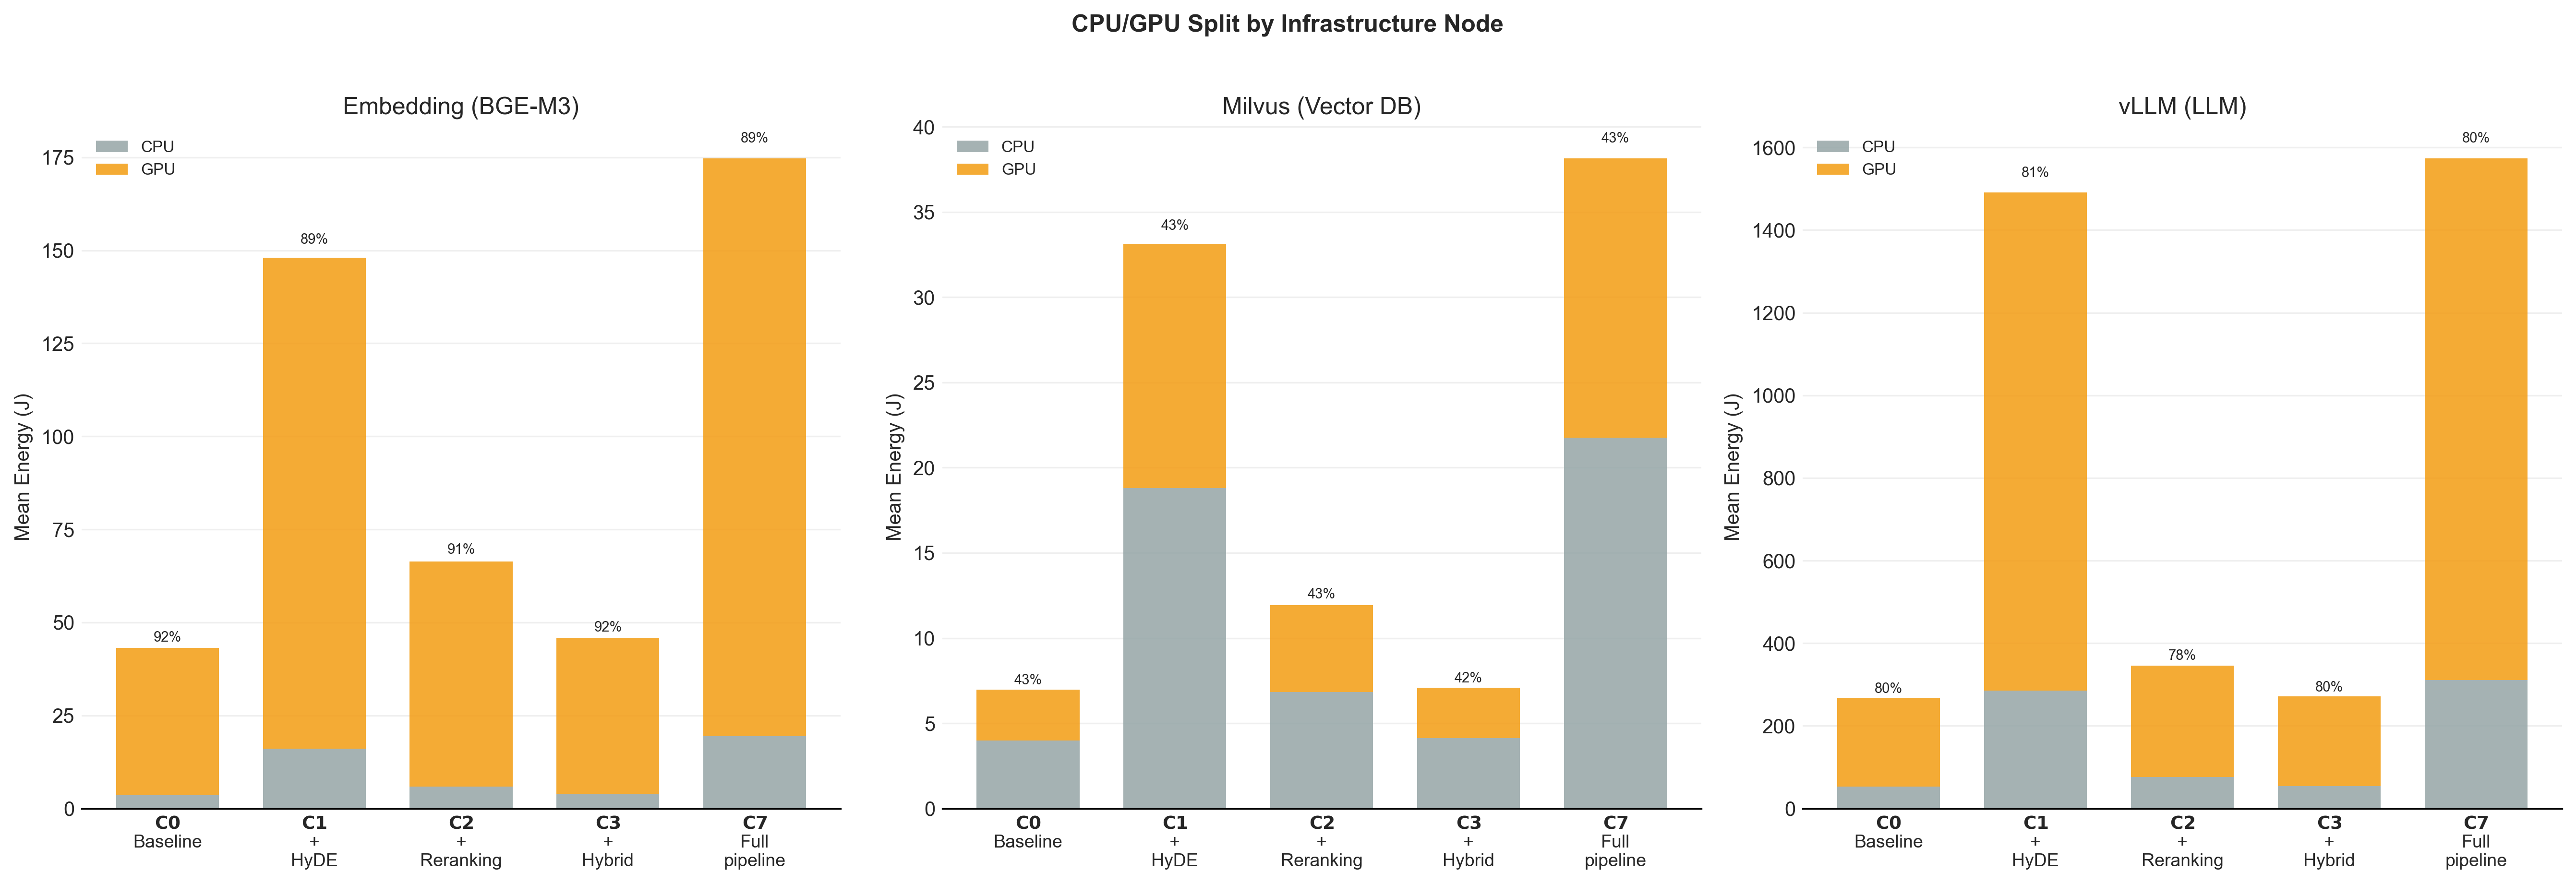
\includegraphics[width=0.95\textwidth]{node_device_faceted.png}
    \caption{CPU/GPU energy split per infrastructure node}
    \label{fig:node-device}
    % Source: hotpot/2-performance/output/plots/node_device_faceted.png
\end{figure}


% --- Distributional view ---

The HotpotQA dataset could in principle produce
different energy profiles across query subtypes.
Figure~\ref{fig:energy-by-querytype} shows that the configuration ranking
holds consistently across both subtypes.
Bridge queries exhibit wider energy distributions than comparison queries,
particularly in HyDE-enabled configurations. 
Paradoxically, they also consume slightly more
energy and latency on average, yet achieve higher retrieval scores (0--1
scale, higher is better).

% --- Section summary ---

In summary, enabling all modules (C7) costs 5.6$\times$ more energy than the
minimal pipeline (C0). The cost is dominated by HyDE's additional LLM
generation pass, which alone adds 1{'}355~J---more than four times the entire
C0 baseline. Module costs are approximately additive and consistent across
query subtypes. The LLM node carries 84--88\% of total energy, though hardware
utilization differs by node: GPU-dominated for LLM and embedding, CPU-heavy
for vector retrieval. 
% Section~\ref{subsec:latency-energy} 

\begin{figure}[h!]
    \centering
    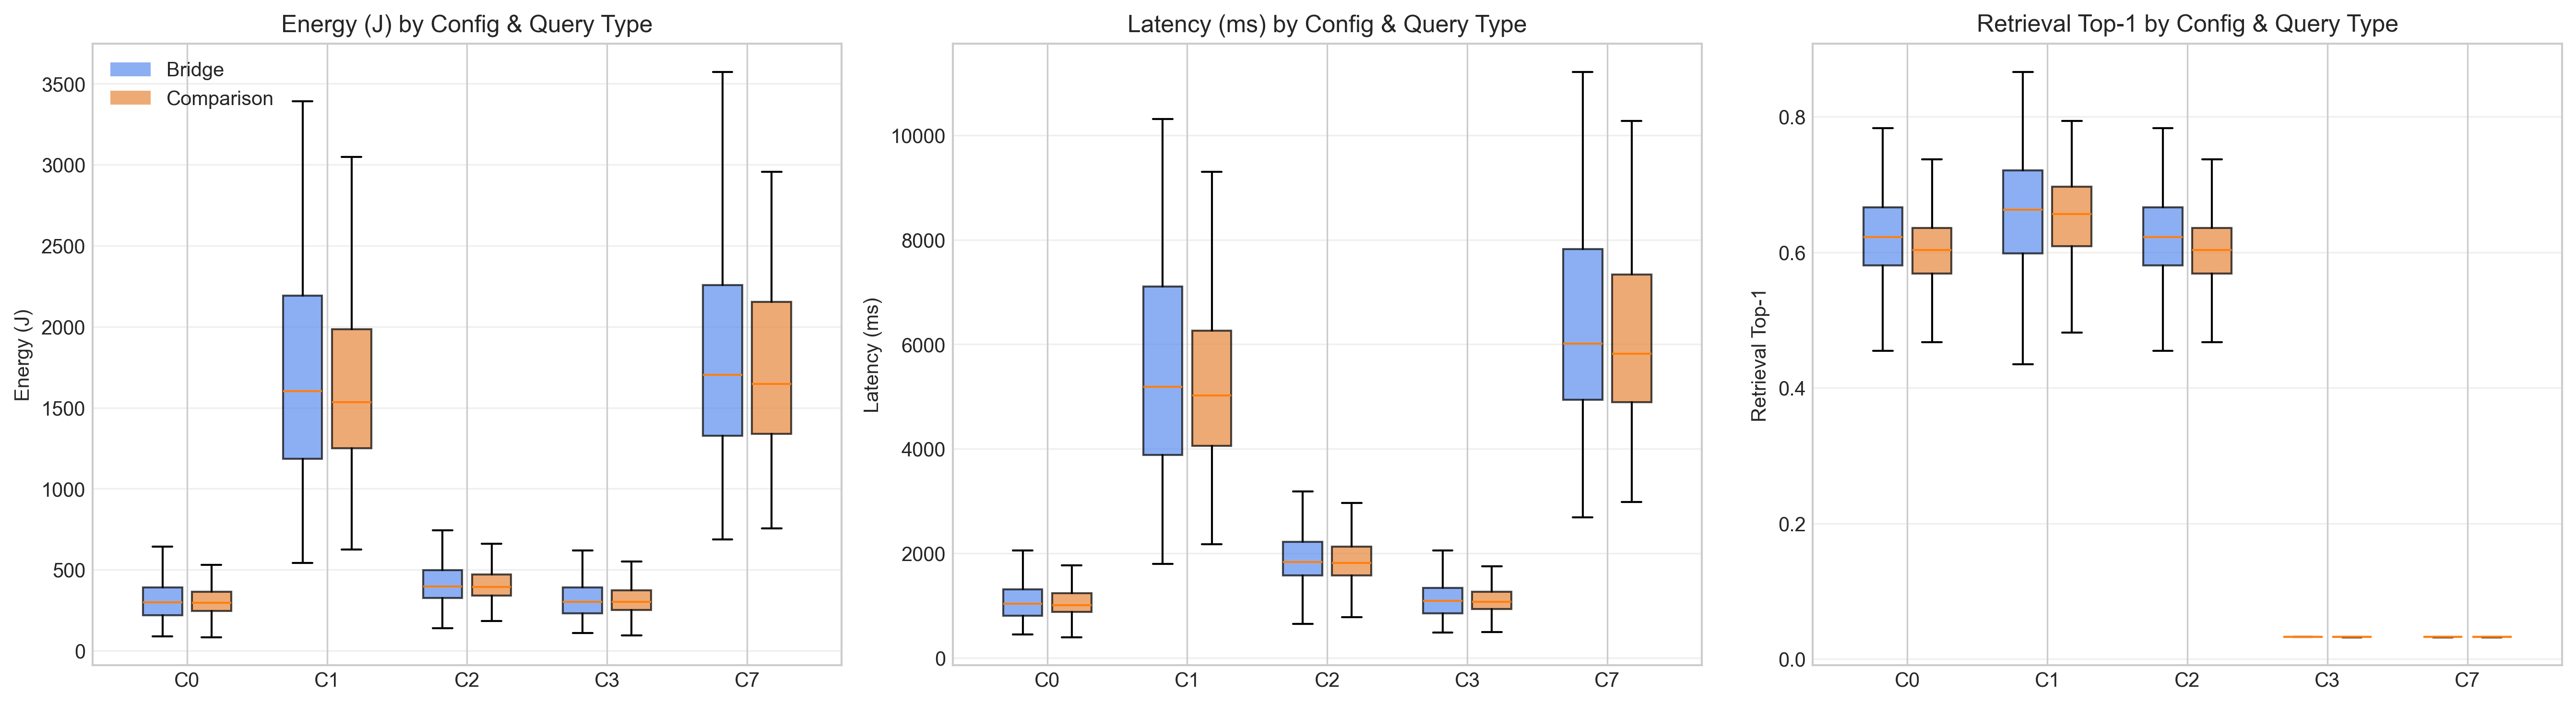
\includegraphics[width=0.9\textwidth]{energy_by_query_type.png}
    \caption{Energy distribution by query subtype}
    \label{fig:energy-by-querytype}
    % Source: hotpot/2-performance/output/plots/energy_by_query_type.png
\end{figure}

\subsection{Energy-Latency Correlation}
\label{subsec:latency-energy}

% --- Latency by configuration ---
We examine the latency dimension and the relationship between energy and execution time.

The figure below reports the TTFT(left) and response generation time (right). 
the mean TTFT ranges from 982~ms (C0) to 6{'}153~ms (C7); a
6.3$\times$ difference. The latency structure mirrors the energy clusters
from Section~\ref{subsec:energy-breakdown} where C0 and C3 share the lowest TTFT
($\sim$982--1{'}032~ms) followed by reranking configurations, then HyDE configurations 
and then combined configurations around
6{'}109--6{'}153~ms.

The answer generation time is approximately constant across
all configurations ($\sim$112~ms). It confirms that the LLM generation phase
does not vary with retrieval enrichment.

\begin{figure}[h!]
    \centering
    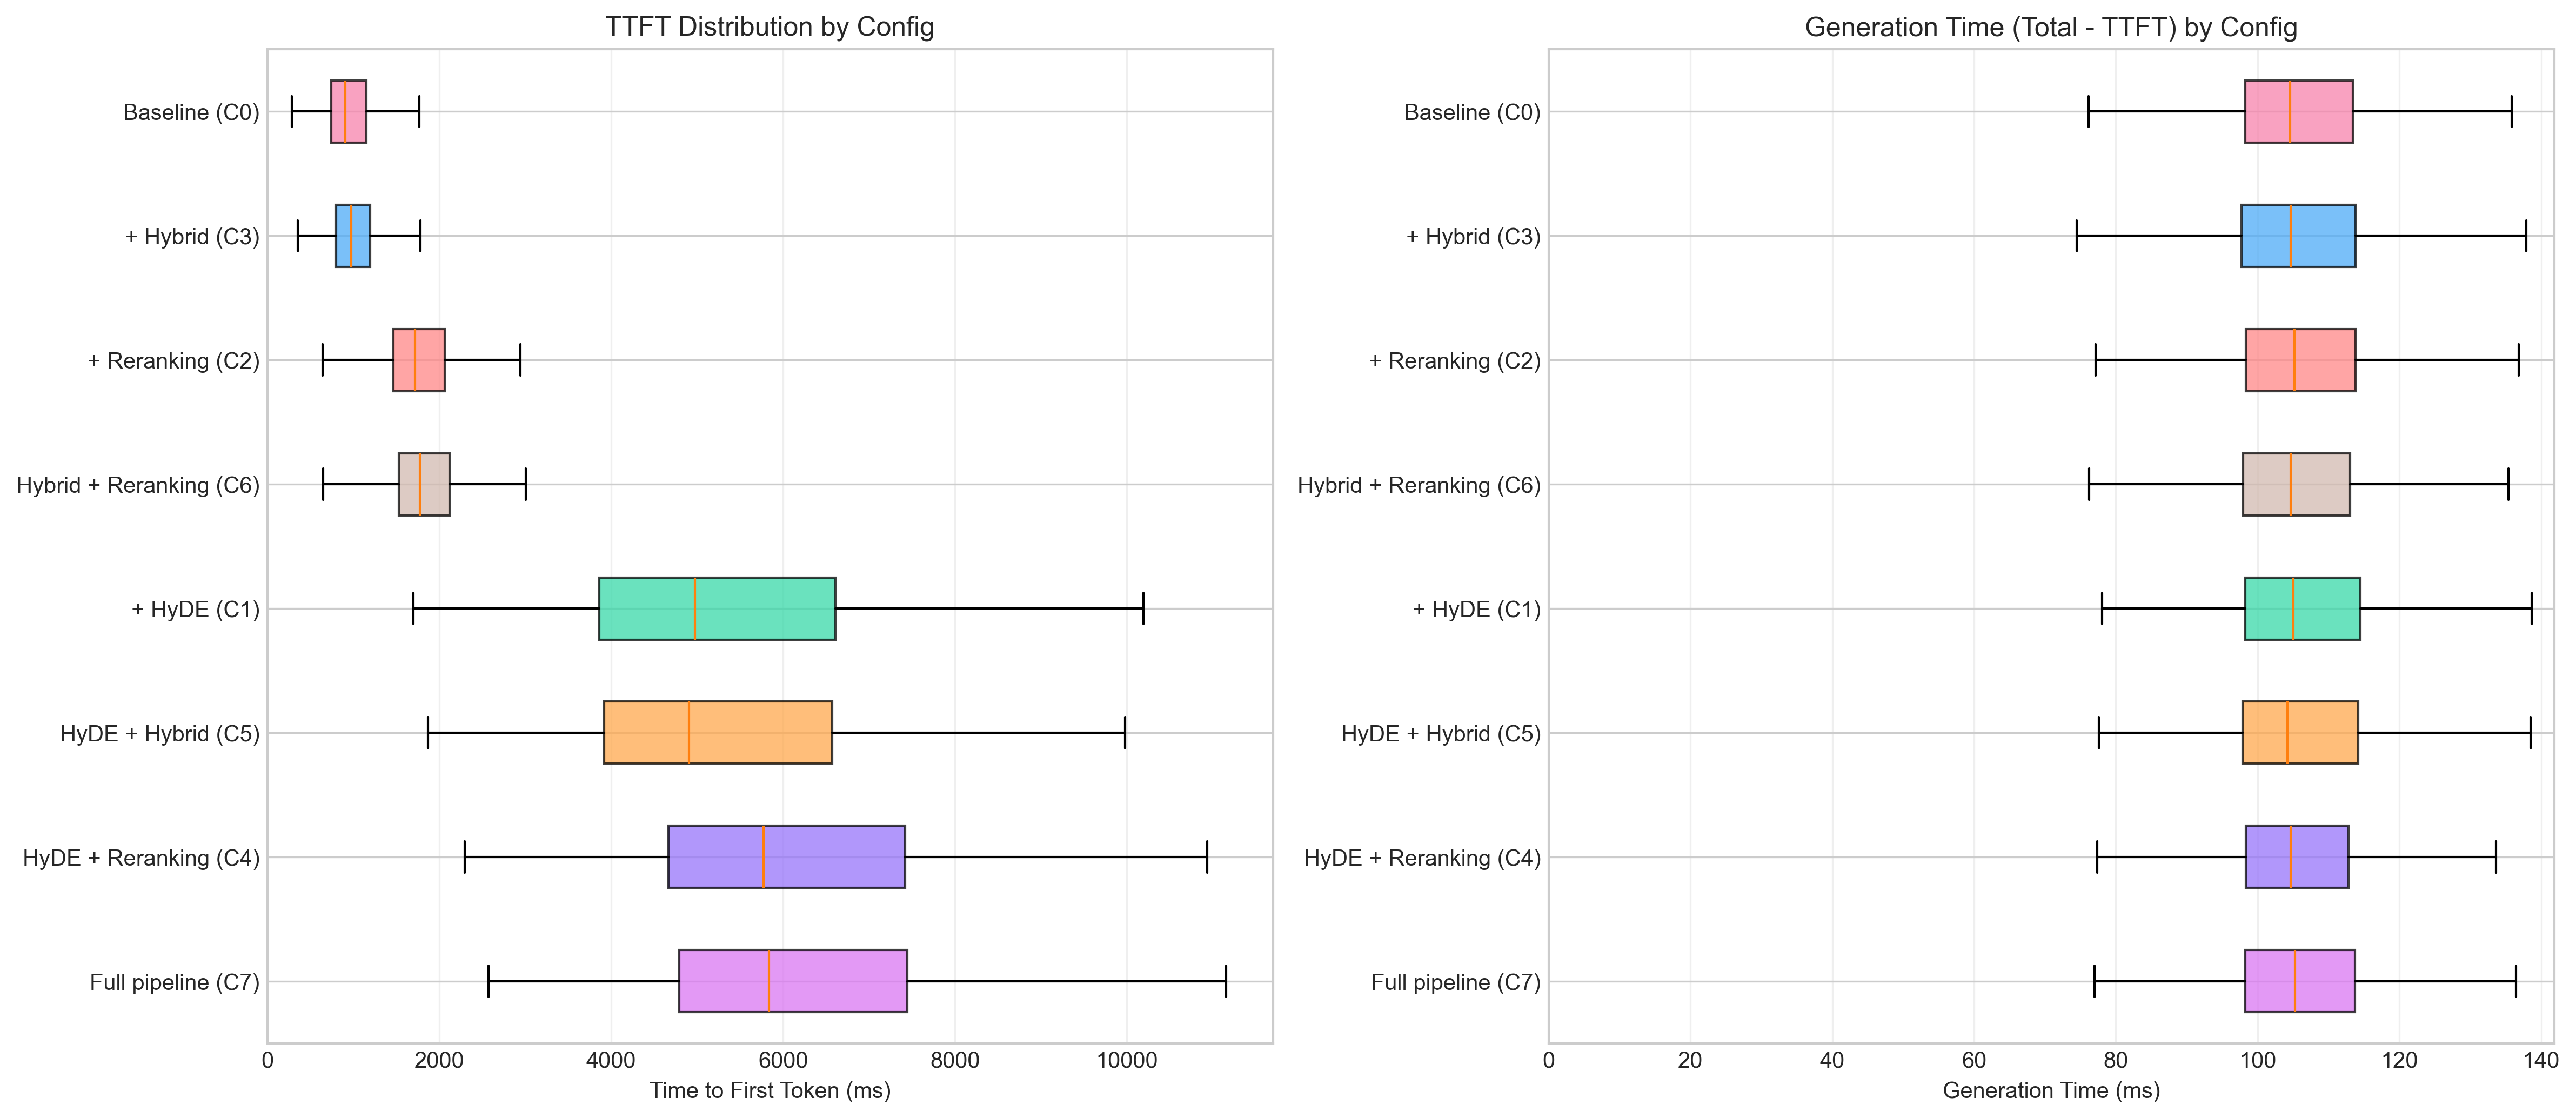
\includegraphics[width=0.9\textwidth]{latency_by_config.png}
    \caption{TTFT and total response time per configuration}
    \label{fig:latency-by-config}
    % Source: hotpot/2-performance/output/plots/latency_by_config.png
\end{figure}

Again, HyDE module imposes the largest TTFT penalty because it requires a complete LLM
generation pass before retrieval can begin. The HyDE adds 4{'}293~ms to TTFT,
reranking adds 825~ms and hybrid adds 50~ms. The combined TTFT of C7
(6{'}153~ms) closely matches the sum of individual deltas
(C0 + HyDE + reranking + hybrid = 982 + 4{'}293 + 825 + 50 = 6{'}150~ms),
confirming that module latencies are again approximately additive.

% --- Cross-dimension cost summary ---

Table~\ref{tab:module-cost} consolidates energy and latency costs per module.
The three modules differ by two orders of magnitude in cost. HyDE
adds 1{'}355~J and 4{'}293~ms; hybrid adds 6~J and 50~ms. This
asymmetry has direct implications for control: hybrid retrieval can be
enabled generously, while HyDE activation must be selective to achieve
meaningful energy savings.

\begin{table}[h!]
\centering
\begin{tabular}{l r r r}
\hline
\textbf{Module} & \textbf{$\Delta$Energy (J)} & \textbf{$\Delta$TTFT (ms)} & \textbf{$\Delta$Total time (ms)} \\
\hline
HyDE              & +1{'}355 & +4{'}293 & +4{'}292 \\
Reranking          & +106     & +825     & +822 \\
Hybrid retrieval   & +6       & +50      & +46 \\
\hline
\end{tabular}
\caption{Per-module marginal cost (C0 delta).}
\label{tab:module-cost}
\end{table}

% --- Energy-latency relationship ---

The parallel structure of energy and latency raises a practical question:
can latency serve as a proxy for energy? Prior work often treats response time
as a stand-in for computational cost; it is straightforward to measure
and directly interpretable. 

To test this assumption, Figure~\ref{fig:energy-latency-regression} plots both total
energy (right panel) and energy per token (left panel) against total response
time for all 9{'}600~sessions. Linear regression of total energy on response
time yields $R^2 = 0.978$ with a slope of 310~J/s---confirming that latency
is a strong first-order proxy. The energy-per-token regression yields a
lower $R^2 = 0.860$, reflecting the additional variance introduced by
token-generation efficiency across configurations.

\begin{figure}[h!]
    \centering
    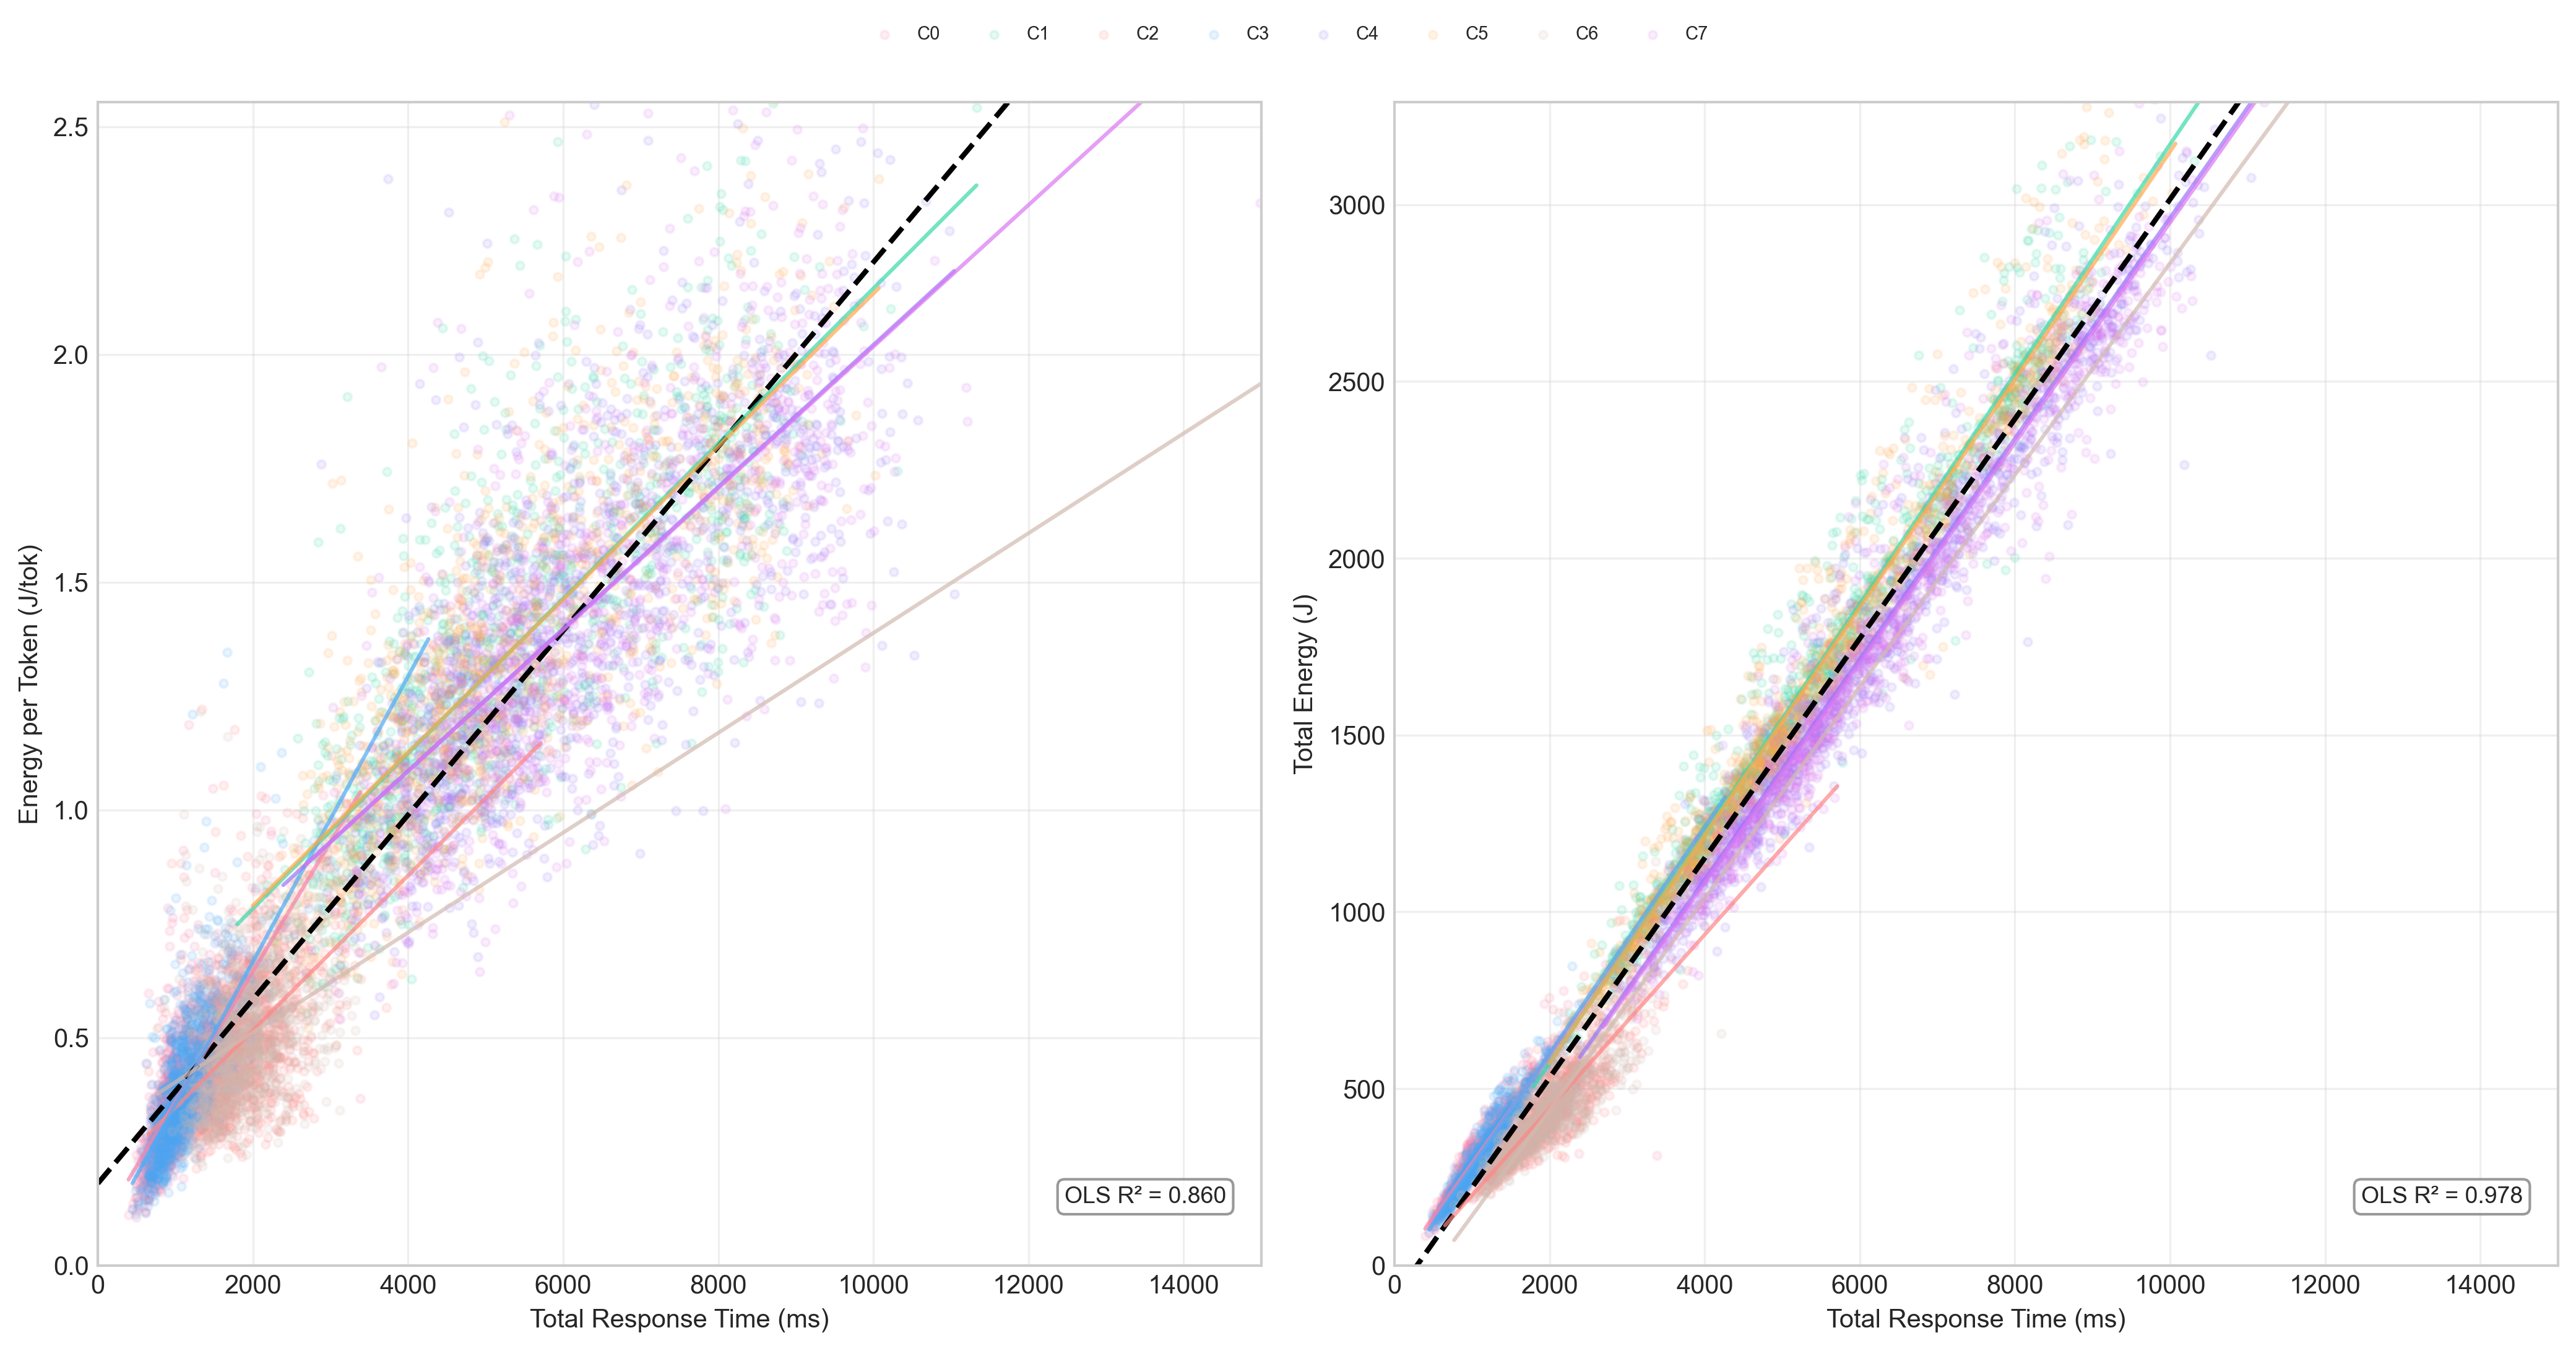
\includegraphics[width=0.95\textwidth]{energy_latency_regression.png}
    \caption{Energy versus total response time}
    \label{fig:energy-latency-regression}
    % Source: hotpot/2-performance/output/plots/energy_latency_regression.png
    %    across 9{'}600~sessions. Left:energy per token versus: total response time ($R^2 = 0.860$). Right: totalenergy versus total response time ($R^2 = 0.978$). The global correlationis strong, but per-configuration slopes (colored lines) diverge.
\end{figure}

The 12-point gap between the two $R^2$ values (0.978 vs 0.860) shows that
latency is a good but imperfect proxy for per-token energy cost. Configurations that
activate reranking draw less instantaneous power than those that invoke HyDE; a 
cross-encoder pass is less GPU-intensive than a full LLM generation
step. 
%Two sessions with identical latency can therefore differ in energy per
%token.

Most studies report only latency; fewer measure total energy, as power
instrumentation is not straightforward. Rago et al.~\cite{rago2025}
recommended energy per token (J/tok) as an energy metric but listed
it as future work only.
% Our setup implements this metric; the $R^2 = 0.860$
% result confirms that it captures variance that latency alone misses.

% --- Energy-latency residuals ---
\begin{figure}[h!]
    \centering
    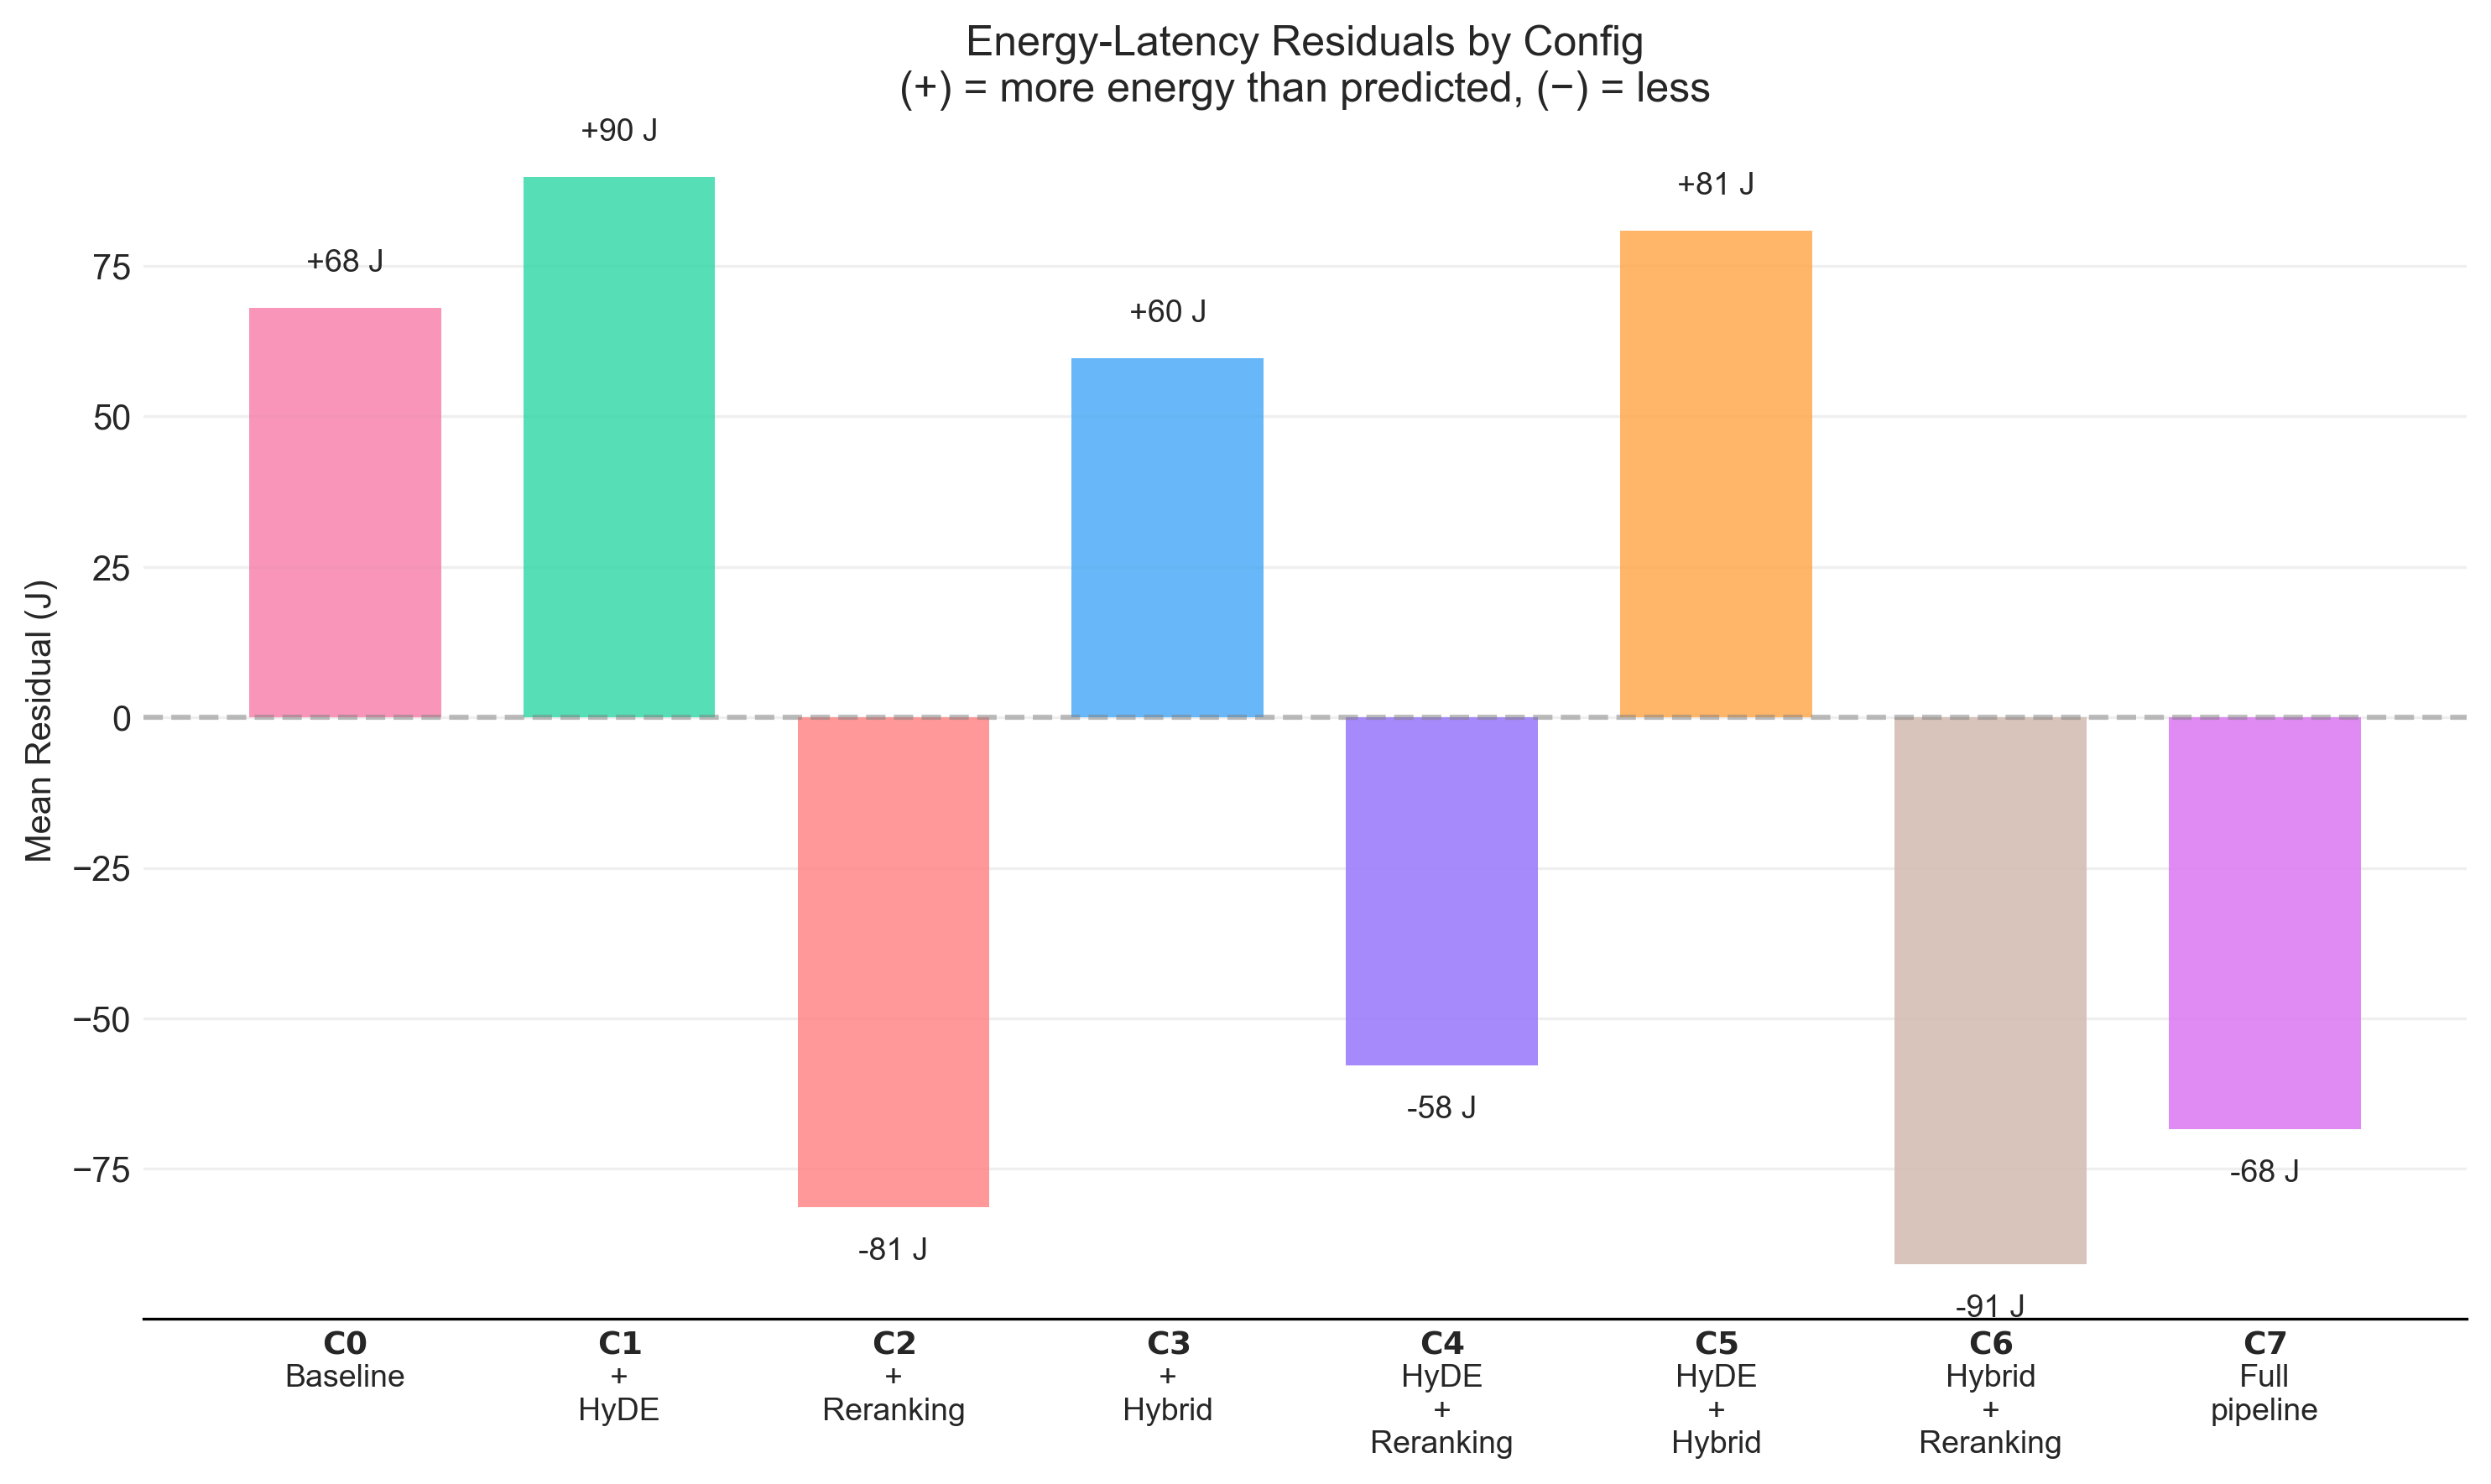
\includegraphics[width=0.8\textwidth]{energy_latency_residuals.png}
    \caption{Energy--latency residuals by configuration}
    \label{fig:energy-latency-residuals}
    % Source: hotpot/2-performance/output/plots/energy_latency_residuals.png
\end{figure}

The figure below makes the deviation explicit.
Reranking configurations (C2, C6) consume 81--91~J \emph{less} energy than
predicted by their latency, while non-reranking configurations (C0, C1, C3,
C5) consume 60--90~J \emph{more} than predicted. 

Positive values indicate configurations that consume more energy than predicted by their
latency; negative values indicate power-frugal configurations. The residuals expose two
distinct hardware utilization regimes:

\begin{itemize}
    \item reranking is ``power-frugal'' (lower GPU intensity from the cross-encoder) 
    \item HyDE is ``GPU-intensive'' (sustained GPU utilization for an additional LLM call). 
\end{itemize}

% Power draw (defined as $E_\text{total} / t_\text{total}$) ranges
% from 217~W (C6) to 309~W (C1), a 40\% spread.


Latency is therefore a good proxy for fast energy
approximation or when direct measurement is impractical.
Guo~et~al.~\cite{keplerenergy2026} reach a similar conclusion in their RAG
experiment and caution that ``the relationship is not perfectly linear.'' Our
results do not improve on this approximation, but they quantify the deviation:
two configurations with equal latency can, in our case differ by up to 
40\% in energy. For accurate per-query cost attribution, energy per token is a more precise
metric; accounts for both power draw variation and output length.

% --- Energy per token vs latency ---
\begin{figure}[h!]
    \centering
    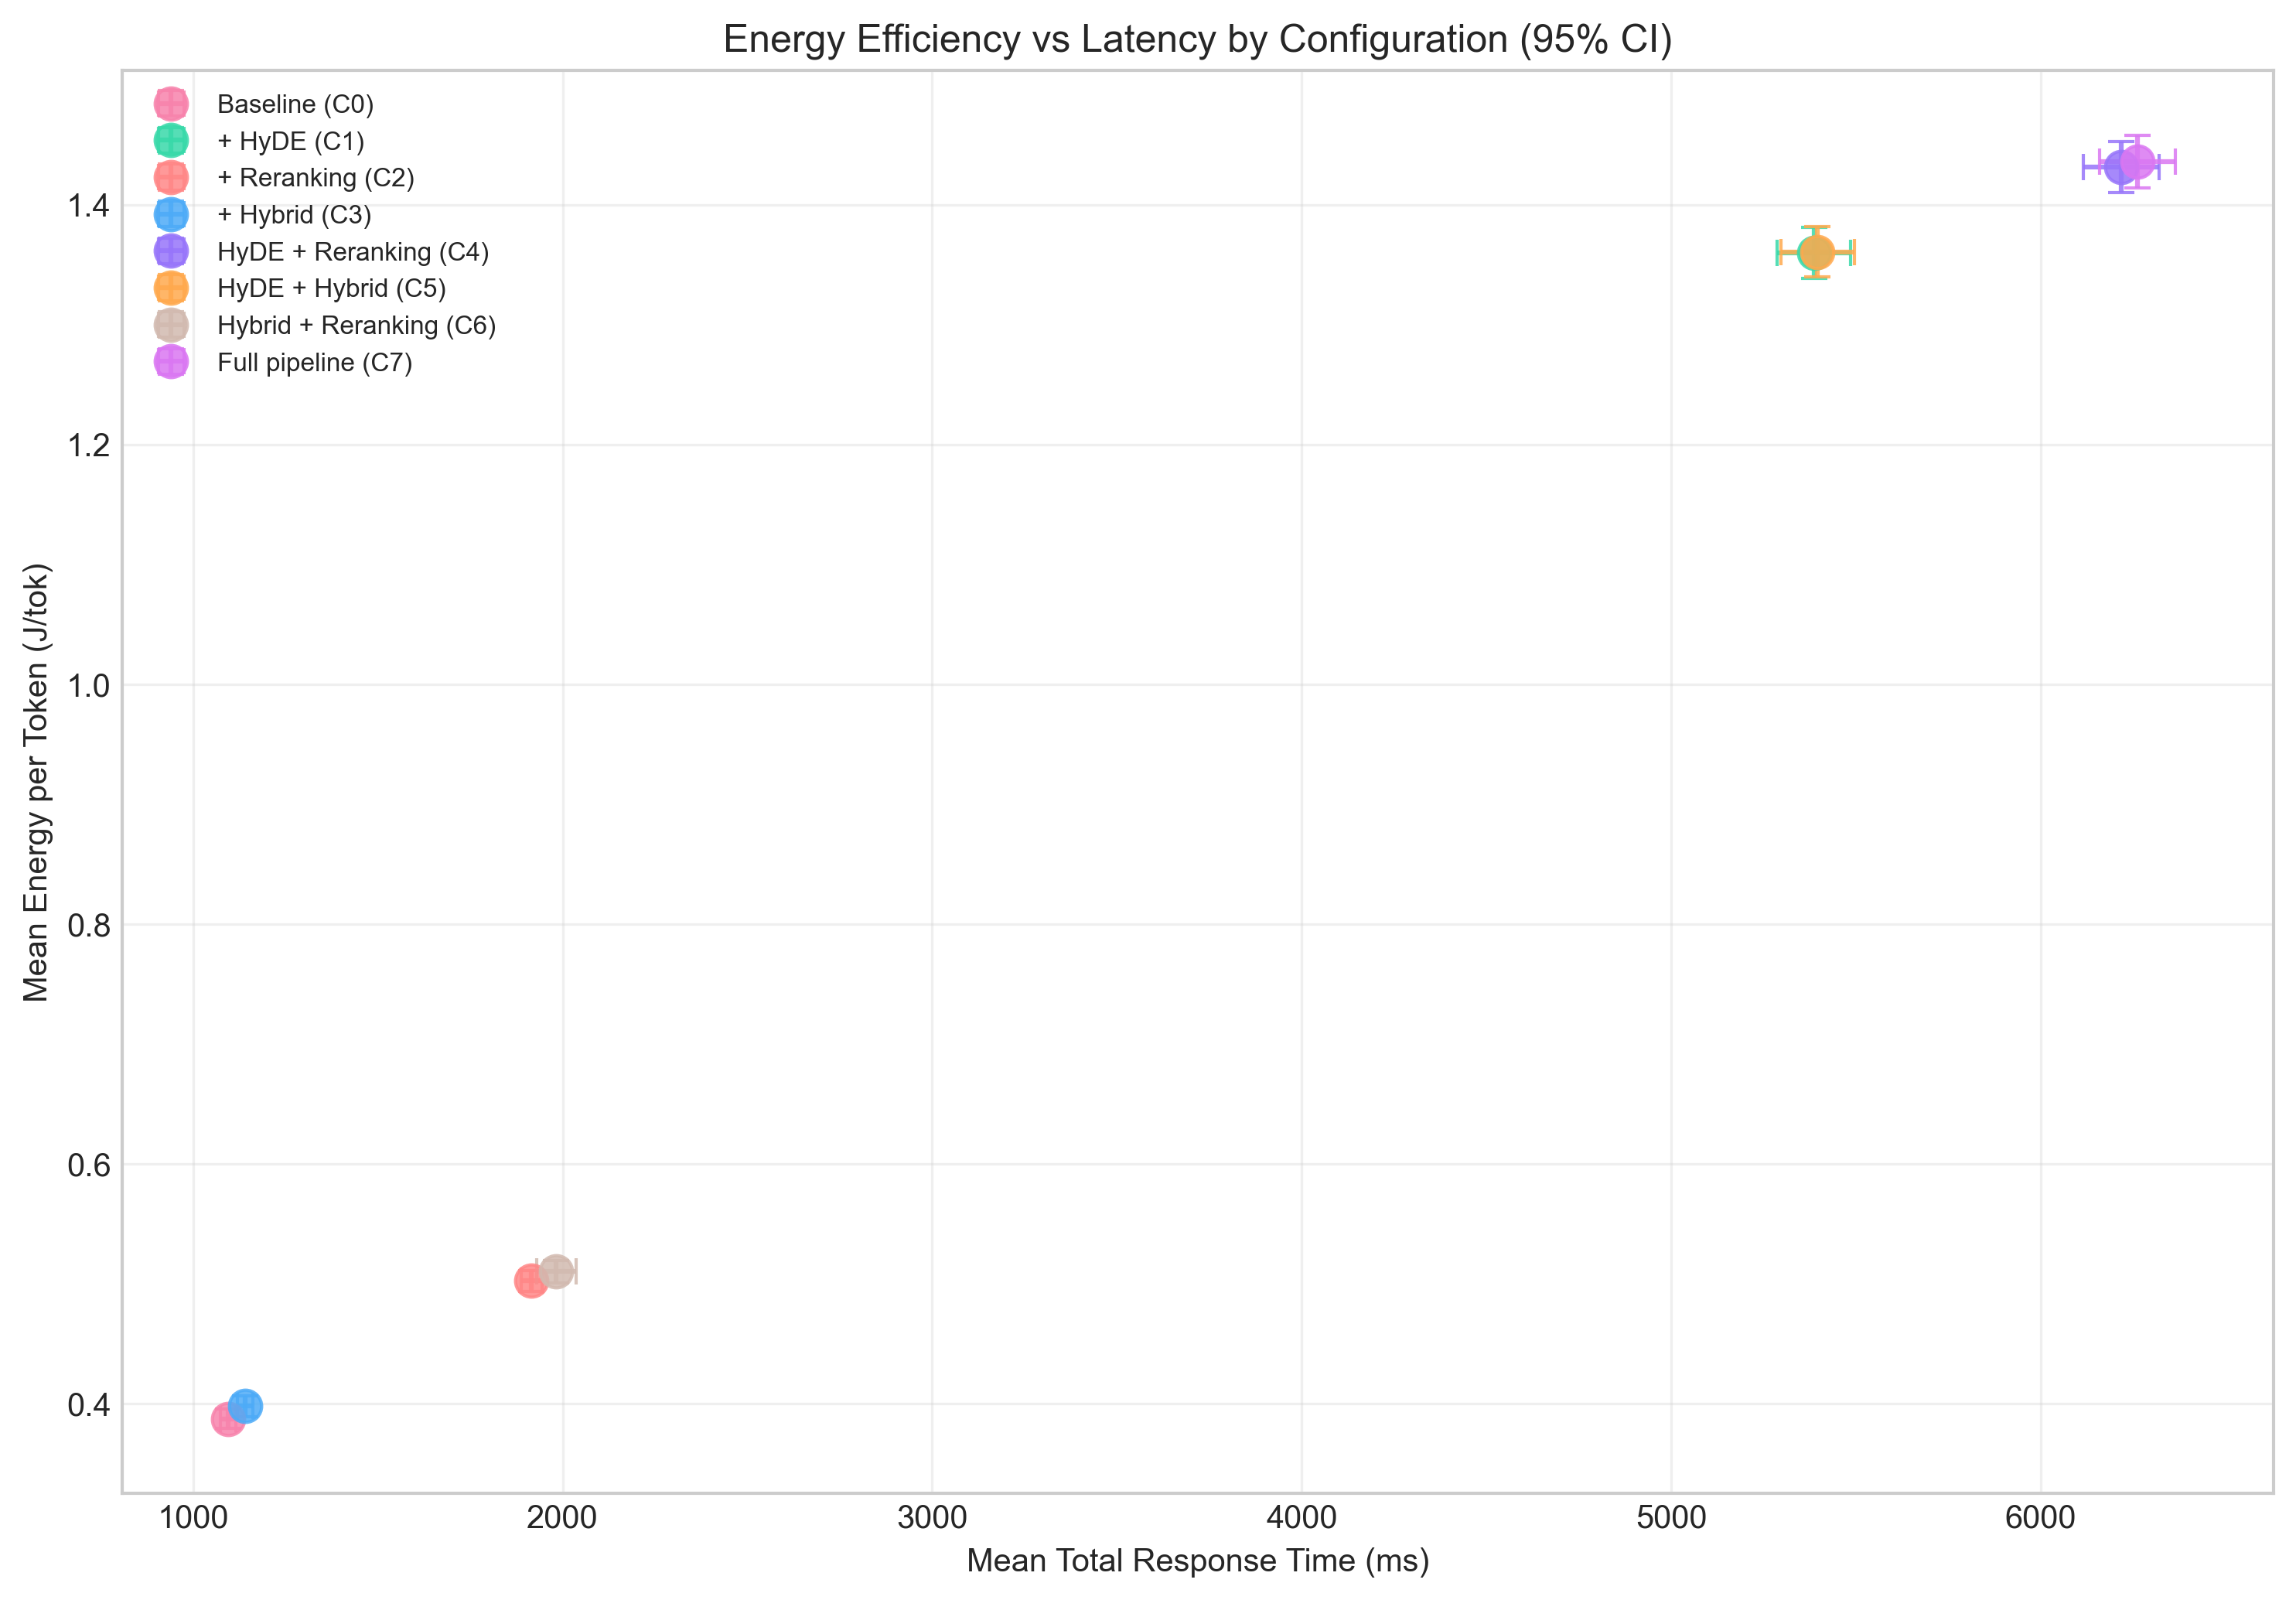
\includegraphics[width=0.8\textwidth]{energy_per_token_vs_latency.png}
    \caption{Energy per token versus total response time}
    \label{fig:energy-per-token}
    % Source: hotpot/2-performance/output/plots/energy_per_token_vs_latency.png
    % HyDE-containing configurations cluster in the high-cost region even after normalization.m n
\end{figure} 

Figure~\ref{fig:energy-per-token} illustrates this point. The baseline consumes
0.39~J/token while the full pipeline consumes 1.44~J/token---a 3.7$\times$ ratio.
HyDE configurations remain the most expensive after normalization, confirming 
structural overhead rather than a token count artifact.

% HyDE configurations generate additional tokens (the hypothetical document),
% which compresses the ratio from 5.6$\times$ (total energy) to 3.7$\times$
% (J/tok). 

% --- Section summary ---

Module costs are highly asymmetric: HyDE dominates both energy and latency,
reranking imposes moderate cost and hybrid retrieval is nearly free. Costs are
approximately additive across modules. The energy-latency relationship is
strong ($R^2 = 0.978$ globally) but configuration-dependent: power draw ranges
from 217~W (reranking) to 309~W (HyDE), so latency alone does not fully
determine energy cost. The energy ordering is more robust under per-token
normalization. Next, we ask whether this cost buys
proportional quality improvement.


\subsection{Quality Trade-offs}
\label{subsec:energy-quality}

% --- Block A: Introducing quality ---

We just established that optional modules impose large and asymmetric energy and
latency overhead. A natural intuition is that these modules improve answer
quality and that the cost is therefore justified. To evaluate this claim, we
examine quality outcomes per configuration using two RAGAS metrics:

\begin{itemize}
    \item \textbf{Faithfulness} fraction of claims supported by retrieved context
    \item \textbf{Factual correctness} semantic agreement with the reference answer
\end{itemize}

These two metrics capture complementary failure modes:
hallucination versus factual error.

% --- Block B: Quality scores across configurations ---

Factual correctness ranges from 0.590 (C5) to 0.633 (C6) across all eight
configurations; a spread of 0.043~points. Faithfulness is wider but still
modest, ranging from 0.771 (C1) to 0.830 (C7); a spread of 0.060~points.
Contrast this with the energy dimension: a 5.6$\times$ energy range produces
less than 6\% of quality variation on either metric. 

\begin{figure}[h!]
    \centering
    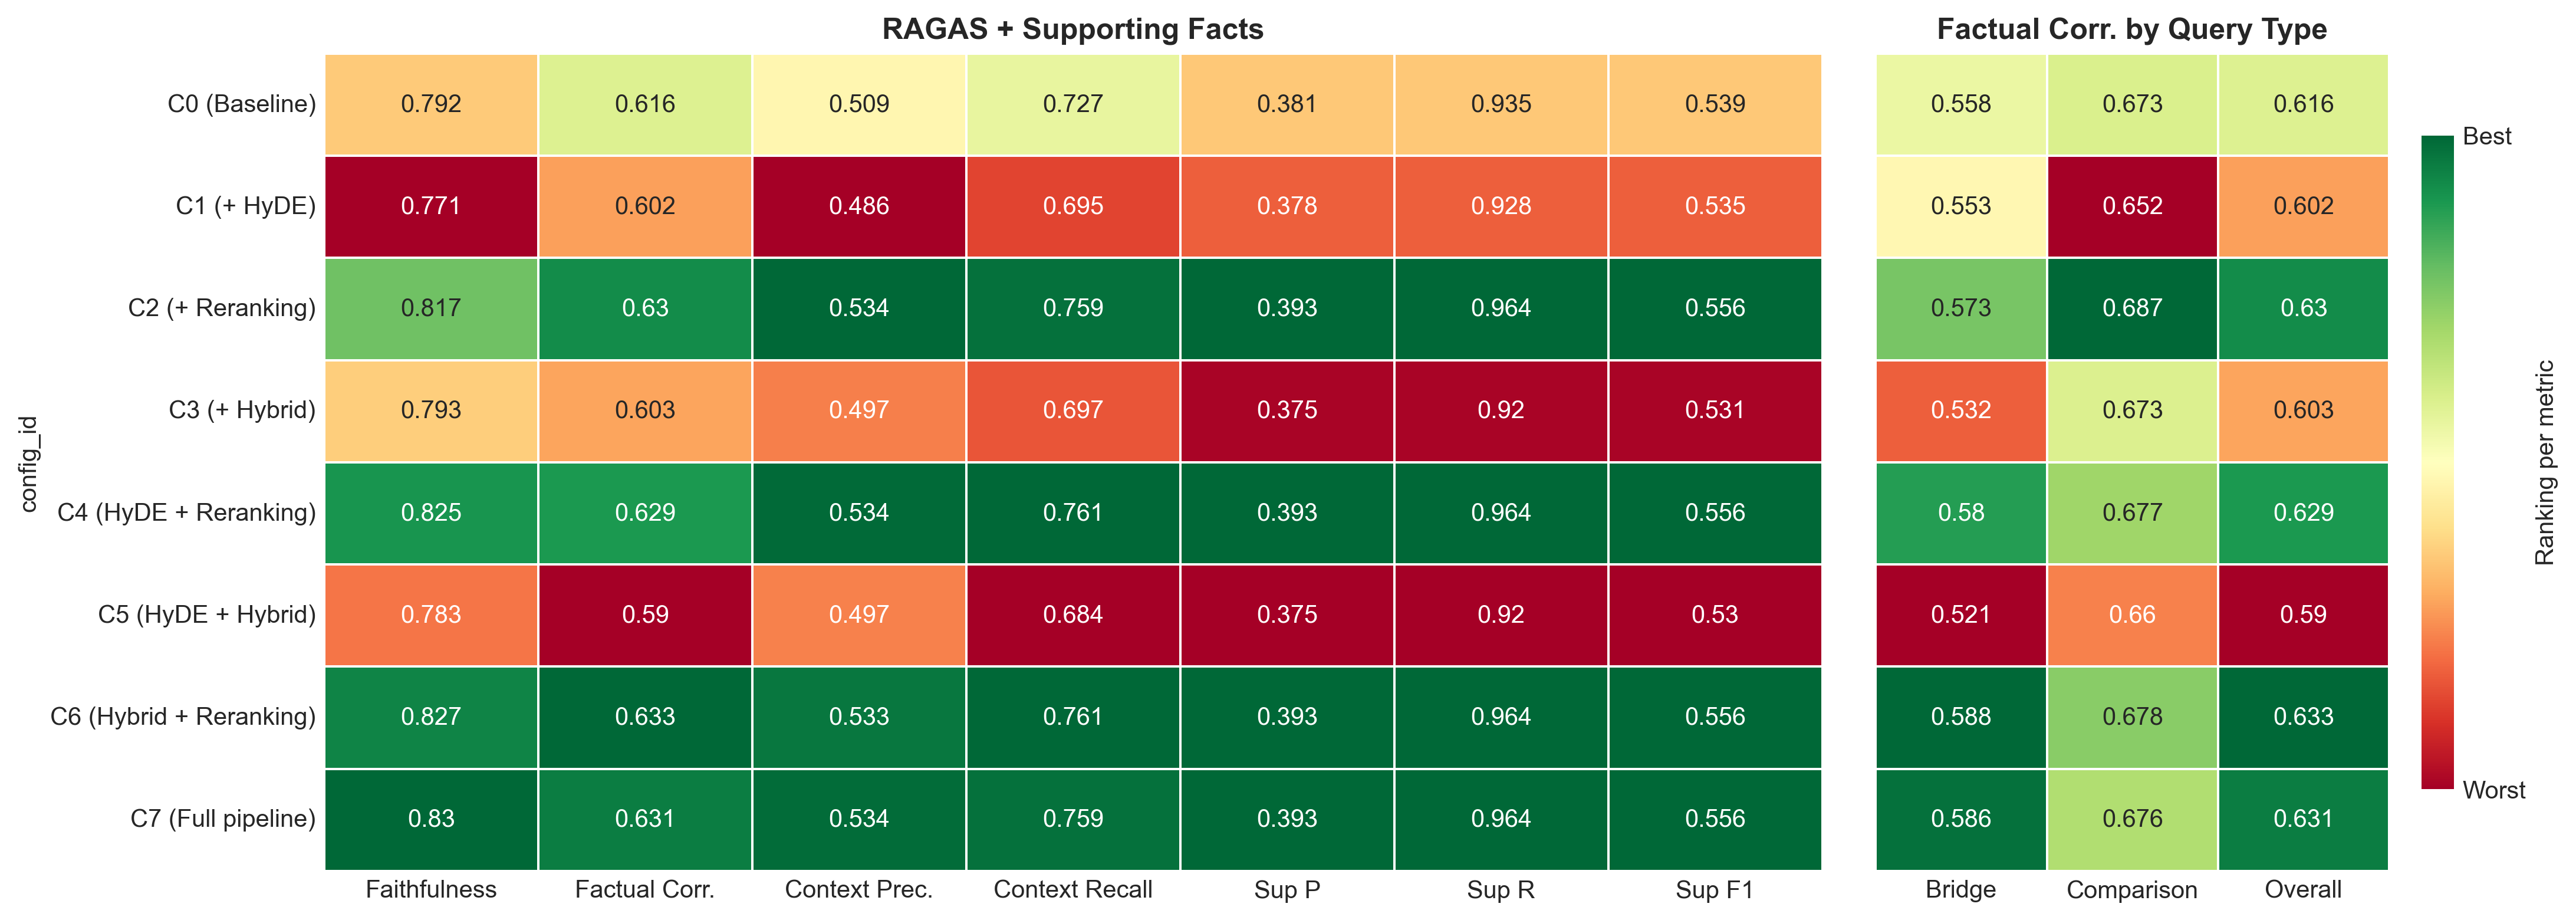
\includegraphics[width=1.0\textwidth]{quality_heatmap_combined.png}
    \caption{Quality deltas from baseline (C0)}
    \label{fig:feature-attribution-quality}
    % Source: hotpot/3-quality/output/plots/feature_attribution_quality.png
    % per pipeline enhancement across four metrics. Reranking consistently improves quality; HyDE consistently degrades it.
\end{figure}

Within-configuration variance dominates between-configuration differences:
the 95\% confidence interval for factual correctness within any single
configuration ($\pm$0.023) covers more than half the cross-configuration
range (0.043). This indicates that query-level difficulty drives quality more
than module activation does.

% --- Block C: Quality varies by query subtype ---

The Figure~\ref{fig:feature-attribution-quality} (right) splits
factual correctness by querysubtype. Comparison queries score consistently higher than bridge queries
across all configurations with a small gap of 0.08--0.15~points. Within each
subtype, reranking configurations (C2, C4, C6, C7) outperform non-reranking
ones. For bridge queries, C6 (hybrid + reranking) achieves the highest score
(0.588), while C5 (HyDE + hybrid) produces the lowest (0.521). For comparison
queries, C2 (reranking only) leads (0.687), while C1 (HyDE only) scores lowest
(0.652).

HyDE degrades quality on both subtypes: comparing each HyDE configuration with
its non-HyDE equivalent yields
factual correctness deltas between $-$0.001 and $-$0.014~points. The effect is
small but consistently negative, meaning HyDE adds substantial energy cost
while providing no quality return on the workload.

The figure~\ref{fig:feature-attribution-quality} generalizes this per-feature
analysis across four quality metrics. Reranking improves all four metrics
(+0.014~fc, +0.025~faithfulness, +0.017~support~F1, +0.032~context recall).
HyDE degrades all four ($-$0.013~fc, $-$0.021~faithfulness,
$-$0.005~support~F1, $-$0.033~context recall). Hybrid retrieval
shows mixed effects: negative on factual correctness ($-$0.013), support~F1 ($-$0.009)
and context recall ($-$0.031) but near-zero on faithfulness.

% --- Block D: Energy-quality tension quantified ---

Table~\ref{tab:energy-quality} compares energy multipliers with quality deltas
for each module. HyDE (C1 versus C0) increases energy by 5.3$\times$ while
\emph{decreasing} average factual correctness by 0.013~points and faithfulness
by 0.021~points. Reranking (C2 versus C0) increases energy by 1.3$\times$ for
quality gains of 0.014 (fc) and 0.025 (faithfulness). Hybrid retrieval (C3
versus C0) increases energy by 1.02$\times$ with a small negative effect on
factual correctness ($-$0.013) and negligible effect on faithfulness (+0.001).

\begin{table}[h!]
\centering
\begin{tabular}{l r r r}
\hline
\textbf{Module} & \textbf{Energy ratio} & \textbf{$\Delta$ Factual corr.} & \textbf{$\Delta$ Faithfulness} \\
\hline
HyDE (C1)       & 5.3$\times$ & $-$0.013 & $-$0.021 \\
Reranking (C2)   & 1.3$\times$ & $+$0.014 & $+$0.025 \\
Hybrid (C3)      & 1.02$\times$ & $-$0.013 & $+$0.001 \\
All (C7)         & 5.6$\times$ & $+$0.016 & $+$0.038 \\
\hline
\end{tabular}
\caption{Energy--quality trade-off per module (C0 delta).}
\label{tab:energy-quality}
\end{table}

The full pipeline (C7) produces a quality improvement of 0.016~points in
factual correctness and 0.038~points in faithfulness at a cost of
5.6$\times$ energy. The quality gain is driven entirely by reranking; HyDE
contributes no positive effect. The relationship between energy investment and
quality return is nonlinear: the first 2\% energy increase (hybrid) yields no
quality improvement, while an additional 31\% (reranking) produces +0.014~fc
and +0.025~faithfulness. The remaining 330\% energy increase from HyDE adds no
further quality benefit.

Figure~\ref{fig:quality-vs-energy-scatter} visualizes this tension. The
x-axis reports mean energy per token (J/tok) rather than total energy to
control for token-count differences introduced by HyDE's additional
generation pass (Section~\ref{subsec:latency-energy}). Two clusters emerge:
non-HyDE configurations (C0, C2, C3, C6) occupy the low-cost region
(0.39--0.51~J/tok), while HyDE configurations (C1, C4, C5, C7) cluster
above 1.36~J/tok with no systematic quality advantage. The Pareto frontier
contains C6 (hybrid + reranking, 0.633~fc at 0.51~J/tok) and C2 (reranking
only, 0.630~fc at 0.50~J/tok).

\begin{figure}[h!]
    \centering
    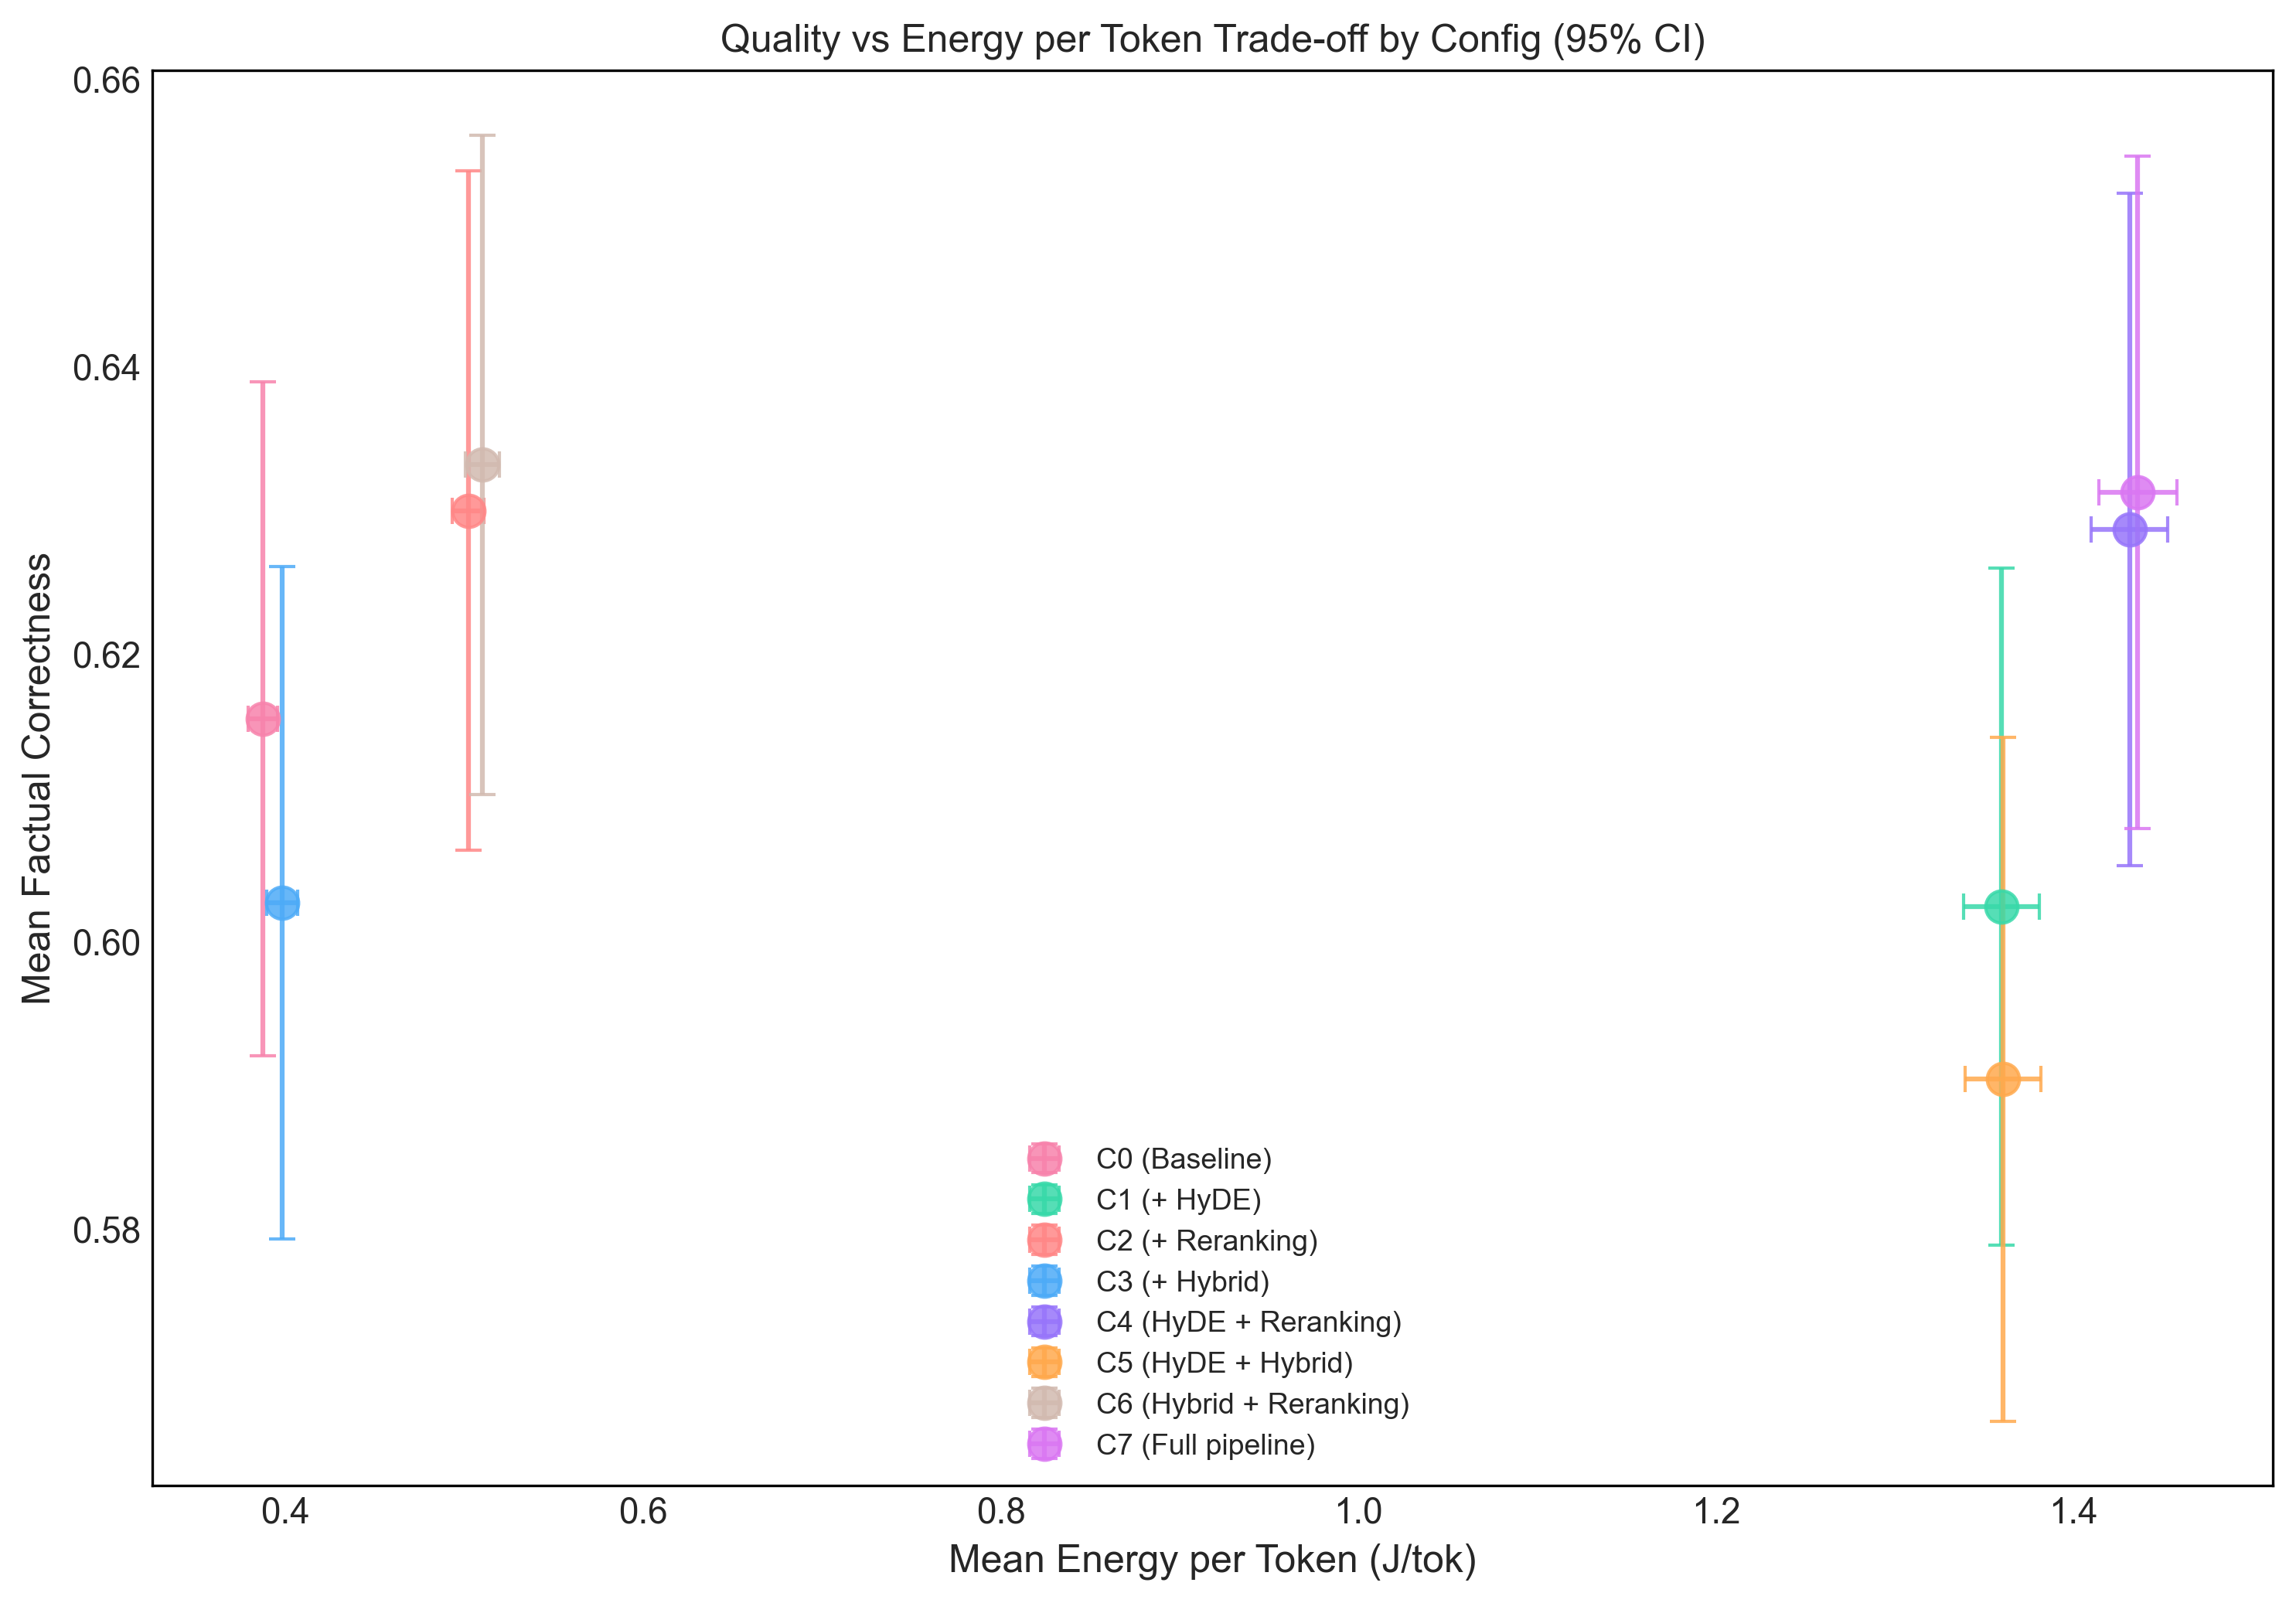
\includegraphics[width=0.85\textwidth]{quality_vs_energy.png}
    \caption{Factual correctness versus energy per token}
    \label{fig:quality-vs-energy-scatter}
    % Source: hotpot/3-quality/output/plots/quality_vs_energy.png
\end{figure}

% --- Block E: Section summary ---

Quality differences across configurations are small (less than 0.06~points on
both metrics) and vary by subtype. Energy differences are large
(5.6$\times$). HyDE produces the worst cost-to-quality ratio: it increases
energy by 5.3$\times$ while degrading both quality metrics. Reranking offers
the best ratio: moderate cost (1.3$\times$) for consistent quality improvement.

In the context of the HotpotQA dataset, HyDE should be disabled by default.
Across all analyses, HyDE is unambiguously negative for this workload:
5.3$\times$ energy, +4{'}293\,ms latency, $-$0.013~factual correctness
and $-$0.021~faithfulness. The effect is consistent across query subtypes
and all four quality metrics. The immediate practical recommendation is to
disable HyDE and operate in the \{C0, C2, C3, C6\}~space.

Within this reduced space, C6 (hybrid + reranking) sits on the Pareto
frontier at 0.633~factual correctness and 435\,J per request---1.37$\times$
C0's energy for the highest quality among non-HyDE configurations. C2
(reranking only) achieves 0.630~fc at 424\,J. The choice between
always-C6 and always-C0 is the most actionable deployment decision: it
requires zero routing infrastructure and captures the quality--energy
trade-off at its sharpest point.

Section~\ref{subsec:hypothesis-validation} synthesizes all three dimensions.


\subsection{Hypothesis Validation}
\label{subsec:hypothesis-validation}

% --- Module-level summary ---

The three preceding sections converge on one pattern: cost is unconditional
but benefit is conditional. Each module exhibits a distinct profile:

\begin{itemize}
    \item \textbf{HyDE}: highest cost (5.3$\times$ energy, 4{'}293~ms
          latency), negative quality effect ($-$0.013~fc, $-$0.021~faith).
    \item \textbf{Reranking}: moderate cost (1.3$\times$ energy, 825~ms
          latency), consistent quality gain (+0.014~fc, +0.025~faith).
    \item \textbf{Hybrid retrieval}: negligible cost (1.02$\times$ energy,
          50~ms latency), near-zero quality effect.
\end{itemize}

% --- The "trivial vs non-trivial" pivot ---

If all modules degraded quality or left it unchanged, the solution would be
straightforward: disable them and collect the energy savings. HyDE does so;
it costs more energy and returns no
quality benefit. Reranking does not; it consistently improves both
faithfulness and factual correctness despite a modest magnitude.
Also, no single configuration dominates across all queries and subtypes.

However, it could be that a module that helps \emph{on average} does not necessarily help every
query and a module that hurts on average may still help specific ones. Whether
per-query patterns exist and whether they are predictable from the query
alone is yet unknown. If module benefit varies across
queries but follows no learnable pattern, then no routing model can outperform
a static rule. The next chapter formalizes this as a decision
problem and investigates whether the available signals support per-query
configuration selection.

\newpage
\section{Configuration Control}
\label{sec:controller}

% Chapter purpose: Formalize the decision problem, define quality labeling,
% quantify the oracle ceiling, characterize available signals.
% All data from HotpotQA (1,199 queries x 8 configs = 9,561 valid sessions).
% No model results — those belong to Chapter 7.


\subsection{Problem Formulation}
\label{subsec:decision-problem}

We showed that optional modules impose
asymmetric costs with inconsistent quality returns. This raises a practical
question: can we choose which modules to activate on a per-query basis, before
executing the pipeline?

\begin{figure}[h!]
\centering
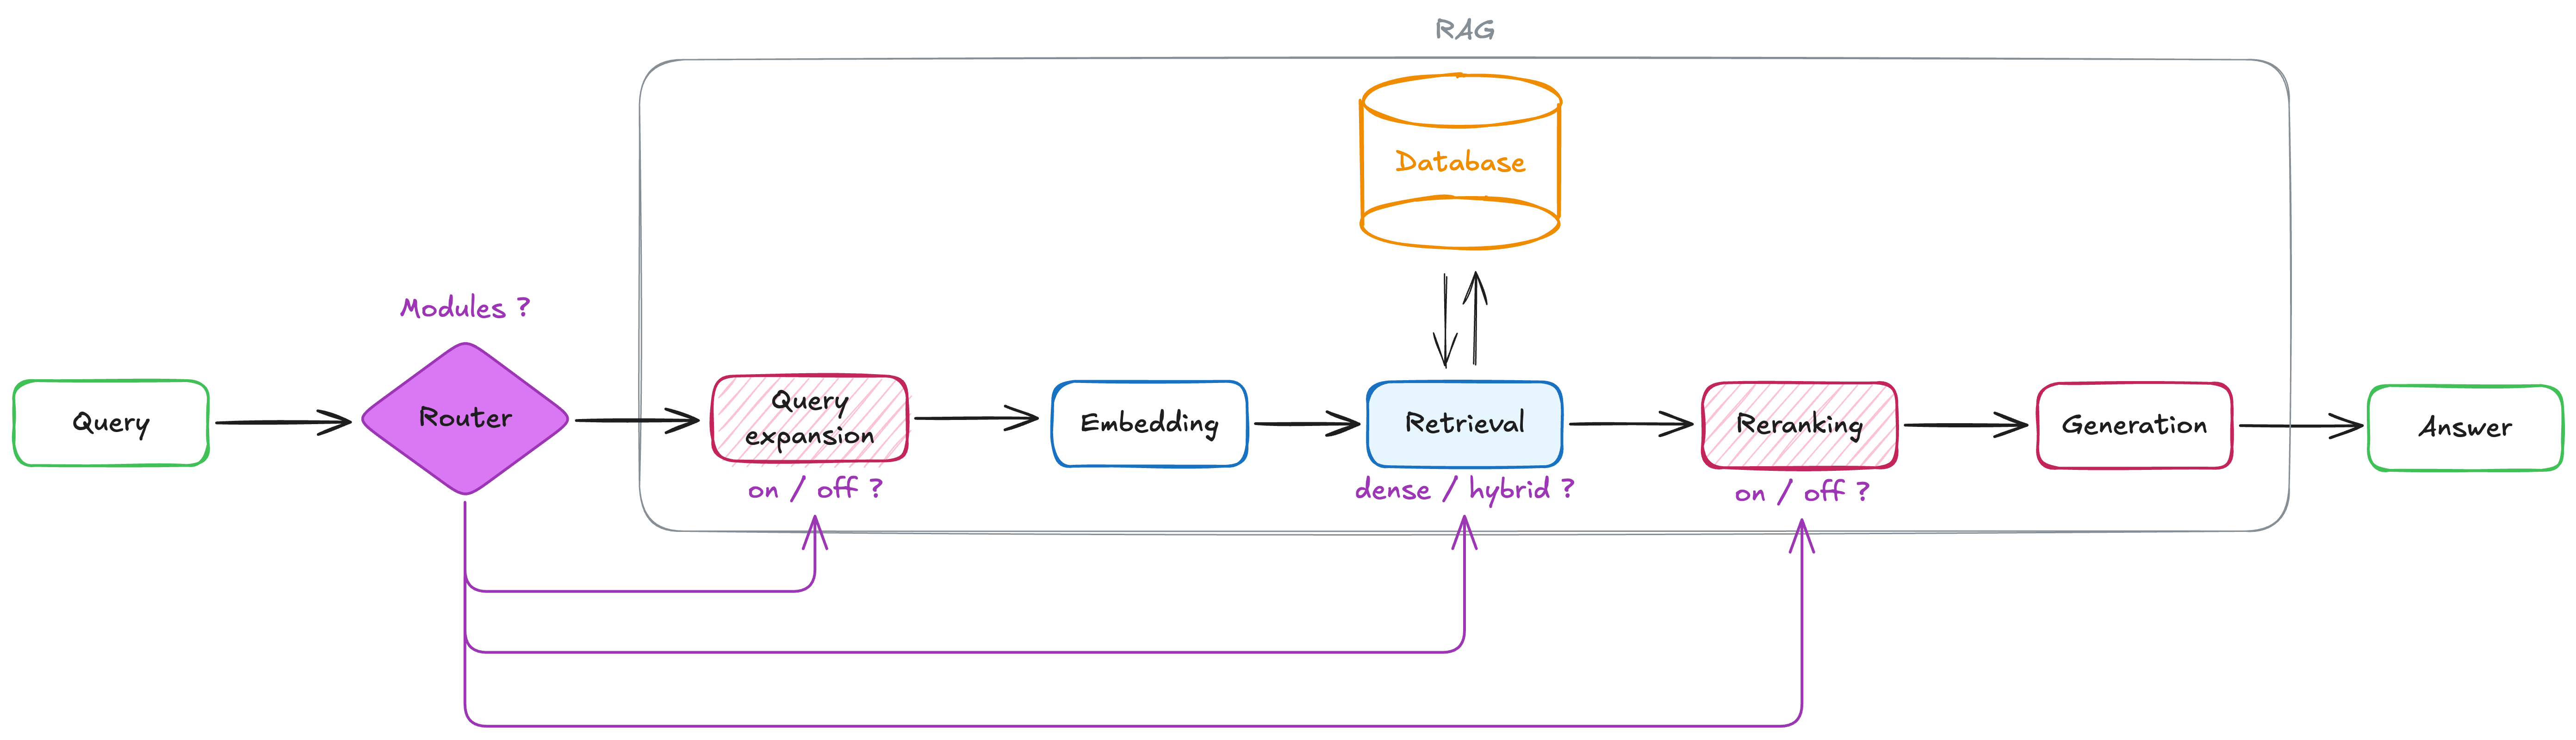
\includegraphics[width=0.85\textwidth]{modules.png}
\caption{Decision process}
\label{fig:decision-process}
\end{figure}

If the sole objective is energy, the answer is trivial: always run C0 (minimal
pipeline) at 318~J per request. No routing model is needed; a static rule
suffices. However, a cheapest-always policy ignores quality. Some queries need
reranking or hybrid retrieval to produce an acceptable answer; routing every
query to C0 sacrifices those responses.

The routing literature addresses this tension through quality-aware selection.
Adaptive-RAG~\cite{adaptiverag2024} classifies query complexity to choose a
retrieval strategy. RouteLLM~\cite{routellm2025} frames model selection as
choosing the cheapest model that exceeds a quality threshold. Our setting is
analogous: among all configurations that produce acceptable quality for a given
query, select the one with the lowest energy cost. We call this the
\emph{cheapest acceptable} principle.

Formally, given a query~$q$, the oracle selects:
%
\begin{equation}
c^*(q) = \arg\min_{c \in \mathcal{C}} \; E(q, c) \quad
\text{subject to} \quad a(q, c) = 1
\label{eq:oracle}
\end{equation}
%
where $E(q,c)$ is the energy consumed by query~$q$ under configuration~$c$, and
$a(q,c) \in \{0,1\}$ indicates whether the response meets an acceptability
threshold. This formulation is an oracle: it requires knowing quality outcomes
before execution.

A practical router $f: \mathcal{X} \to \mathcal{C}$ must predict from
pre-execution query features~$\mathcal{X}$ alone, without observing $E(q,c)$ or
$a(q,c)$. When no configuration is predicted acceptable, the router falls back
to~C7 (all modules enabled) as a safety default.


\subsection{Quality Labeling}
\label{subsec:quality-labeling}

Implementing the cheapest-acceptable principle requires defining
``acceptable.'' This means selecting quality metrics and setting thresholds.

We have 2 metric families available: 
\begin{itemize}
      \item HotpotQA-specific deterministic scores: Answer~F1, Supporting~Facts~F1 and
Joint~F1. They measure token-level and title-level overlap. 
%(Section~\ref{sec:method_protocol})
      \item RAGAS LLM-judged metrics: factual correctness and
faithfulness. They capture semantic agreement and hallucination.
%(Section~\ref{subsec:energy-quality})

\end{itemize}

Table~\ref{tab:hotpot-comparison} shows the quality benchmark scores against
published and source baselines. The Answer~F1 gap is an artefact: our pipeline
generates verbose answers against short-span references, deflating
token-level~F1. Despite an Ans~F1 of 12.1\%, RAGAS factual correctness
averages 0.62, confirming that a majority of answers are semantically correct.
Because the benchmark format mismatch renders Ans~F1 unreliable as a
per-response quality signal and re-conducting the evaluation was not feasible
within the project timeline, we cannot use it for routing labels.

\begin{table}[h!]
\centering
\begin{tabular}{l c c c}
\hline
\textbf{System} & \textbf{Ans F1} & \textbf{Sup F1} & \textbf{Joint F1} \\
\hline
Yang et al.\ (2018) baseline~\cite{hotpotqa2018}
    & 59.02 & 64.49$^\dagger$ & 40.16 \\
% Beam Retrieval~\cite{beamretrieval2024} --- SOTA
%     & 85.04 & 90.09$^\dagger$ & 77.54 \\
\hline
CITI KMS --- best config (C6)
    & 12.1$^\ddagger$ & 55.6$^*$ & 5.1 \\
CITI KMS --- mean over 8 configs
    & 11.7$^\ddagger$ & 54.5$^*$ & 4.9 \\
\hline
\multicolumn{4}{l}{\footnotesize $^\dagger$\,Sentence-level granularity. \;
    $^*$\,Title-level granularity (coarser, not directly comparable).} \\
\multicolumn{4}{l}{\footnotesize $^\ddagger$\,Verbose answers vs.\ short-span references deflate token-level F1.}
\end{tabular}
\caption{HotpotQA distractor-setting quality comparison (F1 scores, \%).}
\label{tab:hotpot-comparison}
\end{table}

% Our system reports the best single-configuration result (C6).
%          Sup is measured at title level for our system and at sentence level
%          for the leaderboard entries.

\paragraph{Metric selection via ICC.}
Metrics can be suited for \emph{system evaluation} (comparing pipelines in
aggregate) and not necessarily for \emph{routing supervision}, which
requires per-query discrimination between configurations. We use the
Intraclass Correlation Coefficient (ICC) to distinguish the two. ICC measures
the fraction of total variance attributable to query identity versus
configuration choice: high ICC means configurations produce nearly identical
scores for a given query, leaving no signal for routing.

Prior work uses deterministic quality metrics---F1, exact match---as
routing supervision signals~\cite{metis2025,adaptiverag2024,routellm2025}.
Our ICC analysis shows that these scores barely change across
configurations for a given query on HotpotQA, making them unsuitable for
routing despite their value in system-level evaluation. Faithfulness
(ICC\,=\,0.432) shows the strongest routing signal among quality metrics.
Post-retrieval scores (context precision, ICC\,=\,0.878) are
query-dominated and provide no discriminative value.

Concretely, Ans~F1 (ICC\,=\,0.825) and Joint~F1 (ICC\,=\,0.822) are
nearly query-determined: for a given query, all configurations produce
near-identical F1 scores. This explains why prior routing work using F1 or
exact-match as supervision targets may overstate routing effectiveness. When
the metric barely varies across configurations, any router appears to
``match'' the oracle.


\begin{table}[h!]
\centering
\begin{tabular}{l c l}
\hline
\textbf{Metric} & \textbf{ICC} & \textbf{Interpretation} \\
\hline
Faithfulness              & 0.432 & Best routing potential \\
Factual correctness       & 0.583 & Moderate routing potential \\
Context recall            & 0.670 & Limited \\
Sup F1                    & 0.695 & Limited \\
Ans F1                    & 0.825 & Query-dominated \\
Joint F1                  & 0.822 & Query-dominated \\
Context precision         & 0.878 & Query-dominated \\
\hline
\end{tabular}
\caption{ICC for candidate routing metrics.}
\label{tab:icc}
\end{table}

Factual correctness and faithfulness carry the between-configuration variance
that routing requires. We use both as a joint acceptability gate.

\paragraph{Metrics distribution.}

\begin{figure}[h]
  \centering
  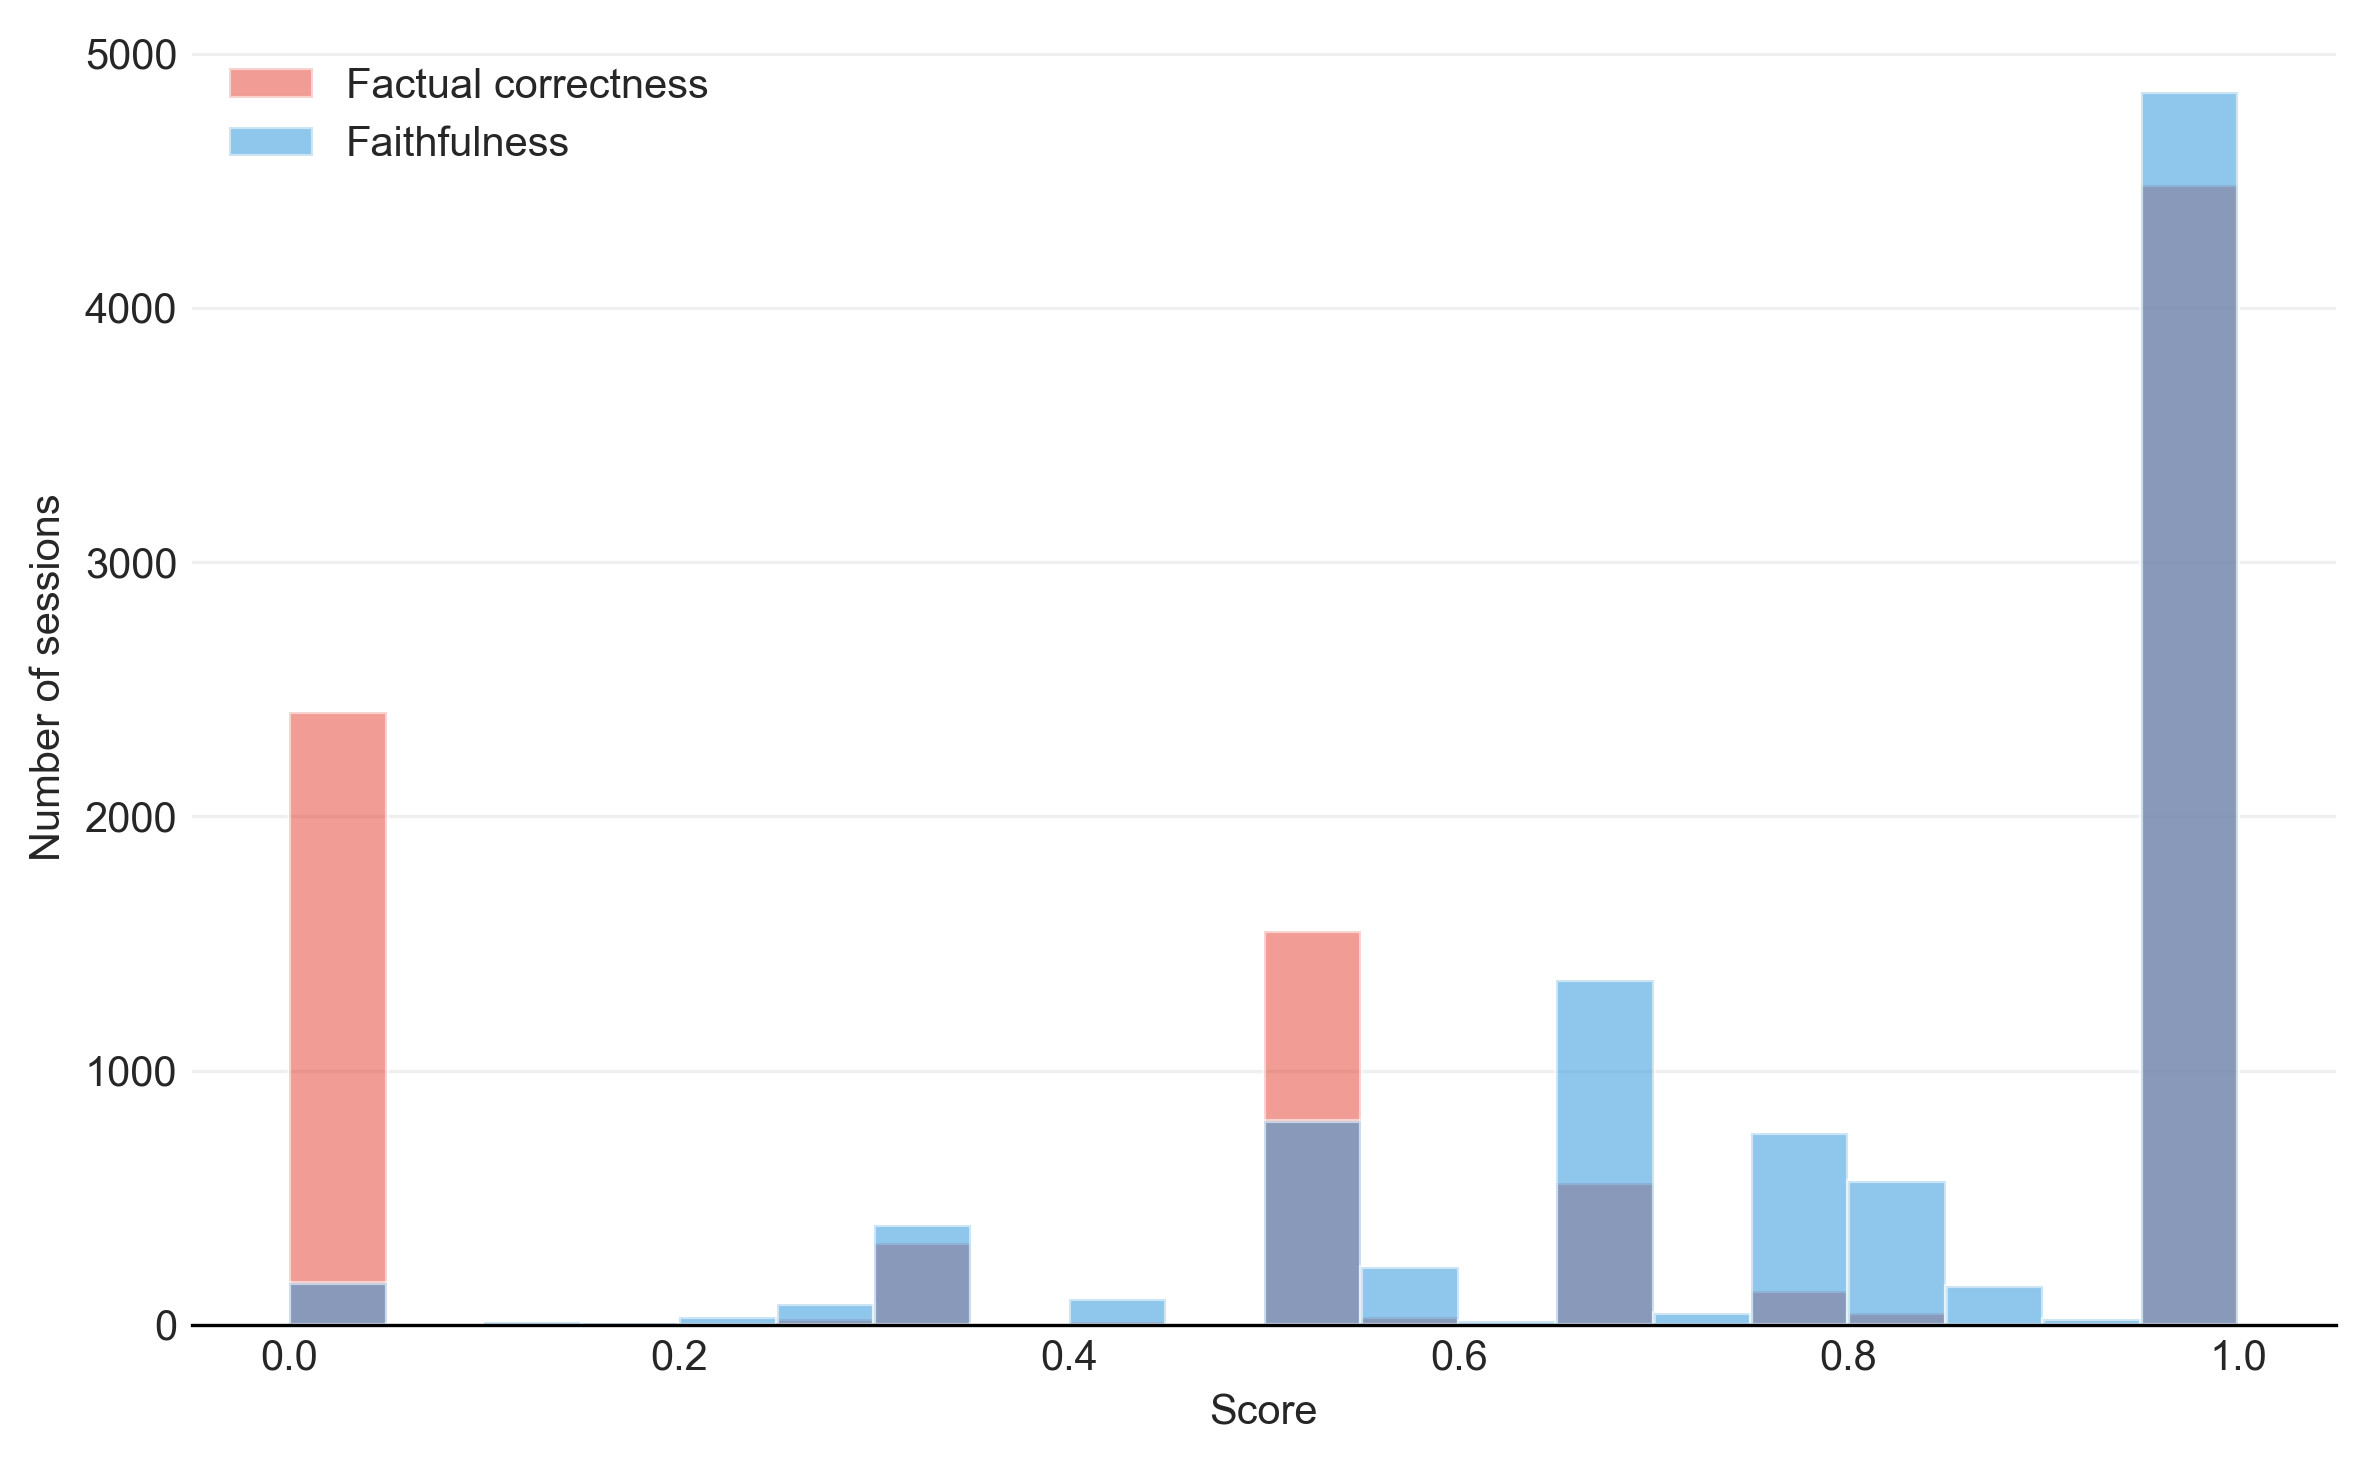
\includegraphics[width=0.90\linewidth]{metrics_distribution.png}
  \caption{Distribution of factual correctness and faithfulness}
  \label{fig:metrics-distribution}
\end{figure}

Faithfulness is bimodal: a dominant cluster at 1.0 indicates that most 
retrieved contexts fully support the generated claims, while a spread of 
lower values captures sessions where the pipeline hallucinates.
Factual correctness follows a broader distribution with a spike at 0.0,
representing queries that every configuration fails and a gradual rise toward higher scores.
These shapes motivate the binary gate below: a threshold must separate the high-score mass 
from the failure tails of both metrics.


\paragraph{Acceptability thresholds.}
A response is \emph{acceptable} if and only if:
%
\begin{equation}
a(q, c) = \mathbf{1}\bigl[\text{fc}(q,c) \geq \tau_{fc}\bigr]
\;\cdot\;
\mathbf{1}\bigl[\text{faith}(q,c) \geq \tau_{faith}\bigr]
\label{eq:acceptability}
\end{equation}


with default thresholds $\tau_{fc} = 0.7$ and $\tau_{faith} = 0.7$.
At 0.7, the label distribution is balanced enough for classification
(C0~38\%, C3~32\%, C2/C6~15\% each); lower thresholds collapse labels
toward~C0. The 70\% floor represents meaningful quality, below it, answers
contain substantive errors, while preserving a routable set of 755~queries
(63\%) sufficient for training.
At these thresholds 33.9\% of sessions (3{'}245 of 9{'}600) pass both criteria.

\paragraph{Label construction.}
For each query~$q$, the label is the cheapest acceptable configuration:

\begin{equation}
\ell(q) = \arg\min_{c \in \mathcal{C}} E(q,c)
\quad \text{subject to} \quad a(q,c) = 1
\label{eq:label}
\end{equation}

When no configuration passes both gates, the optimisation in
Equation~\ref{eq:label} is infeasible: no acceptable routing target exists.
These 445 queries (37.0\%) are excluded from the training set because they
carry no valid supervision signal for the cheapest-acceptable objective.

The routable subset (755 queries, 63.0\%) defines the training population.
C0 accounts for 35.8\% of labels and C3 for 28.6\%; the two cheapest
configurations cover 64\% of routable queries.

\paragraph{Threshold sensitivity.}
The label distribution depends on the chosen thresholds. A $5 \times 5$ grid
sweep over $\tau_{fc} \in [0.6, 1.0]$ and $\tau_{faith} \in [0.6, 1.0]$
produces session pass rates from 25.5\% to 46.9\% and oracle energy savings
from 55.2\% to 65.7\% versus always-C7. The default thresholds sit in the
moderate region. The qualitative pattern (C0 and C3 domination) holds across
all threshold combinations.


\begin{figure}[h!]
    \centering
    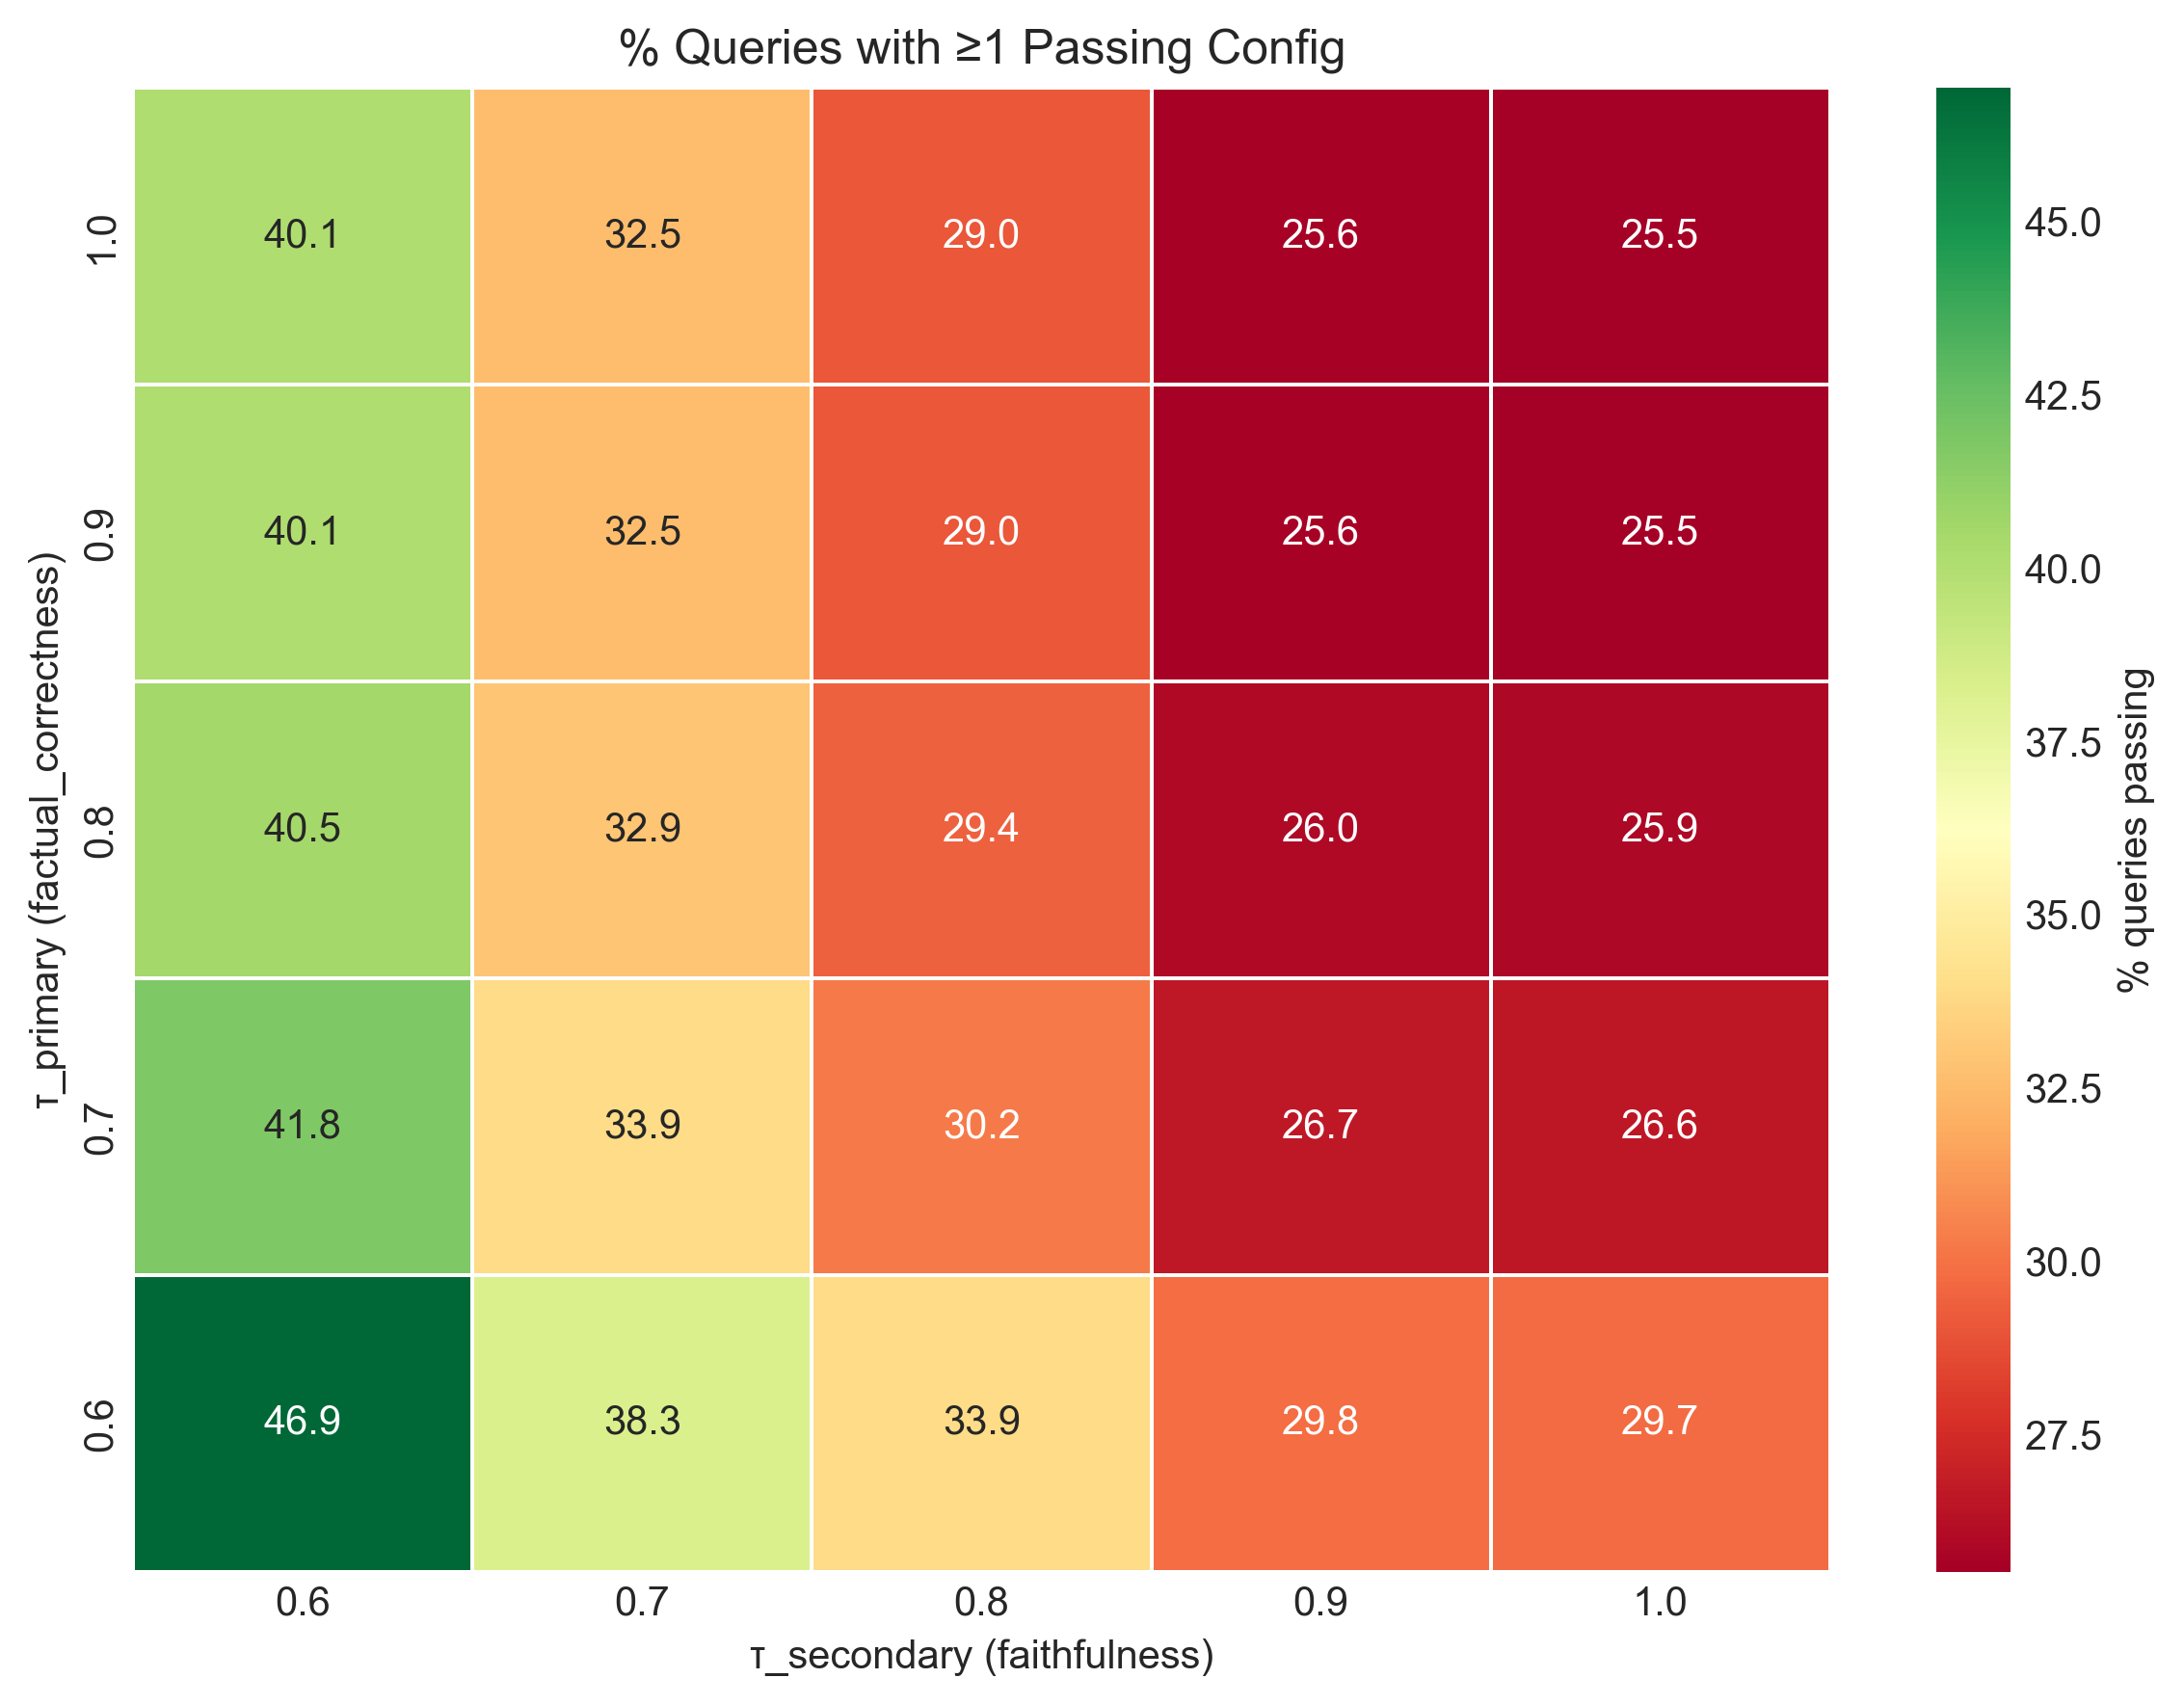
\includegraphics[width=0.85\textwidth]{threshold_pass_rate.png}
    \caption{Session pass rate across threshold combinations}
    \label{fig:label-pass-rate}
    % Source: hotpot/5-label/output/plots/threshold_pass_rate.png
\end{figure}

\begin{figure}[h!]
    \centering
    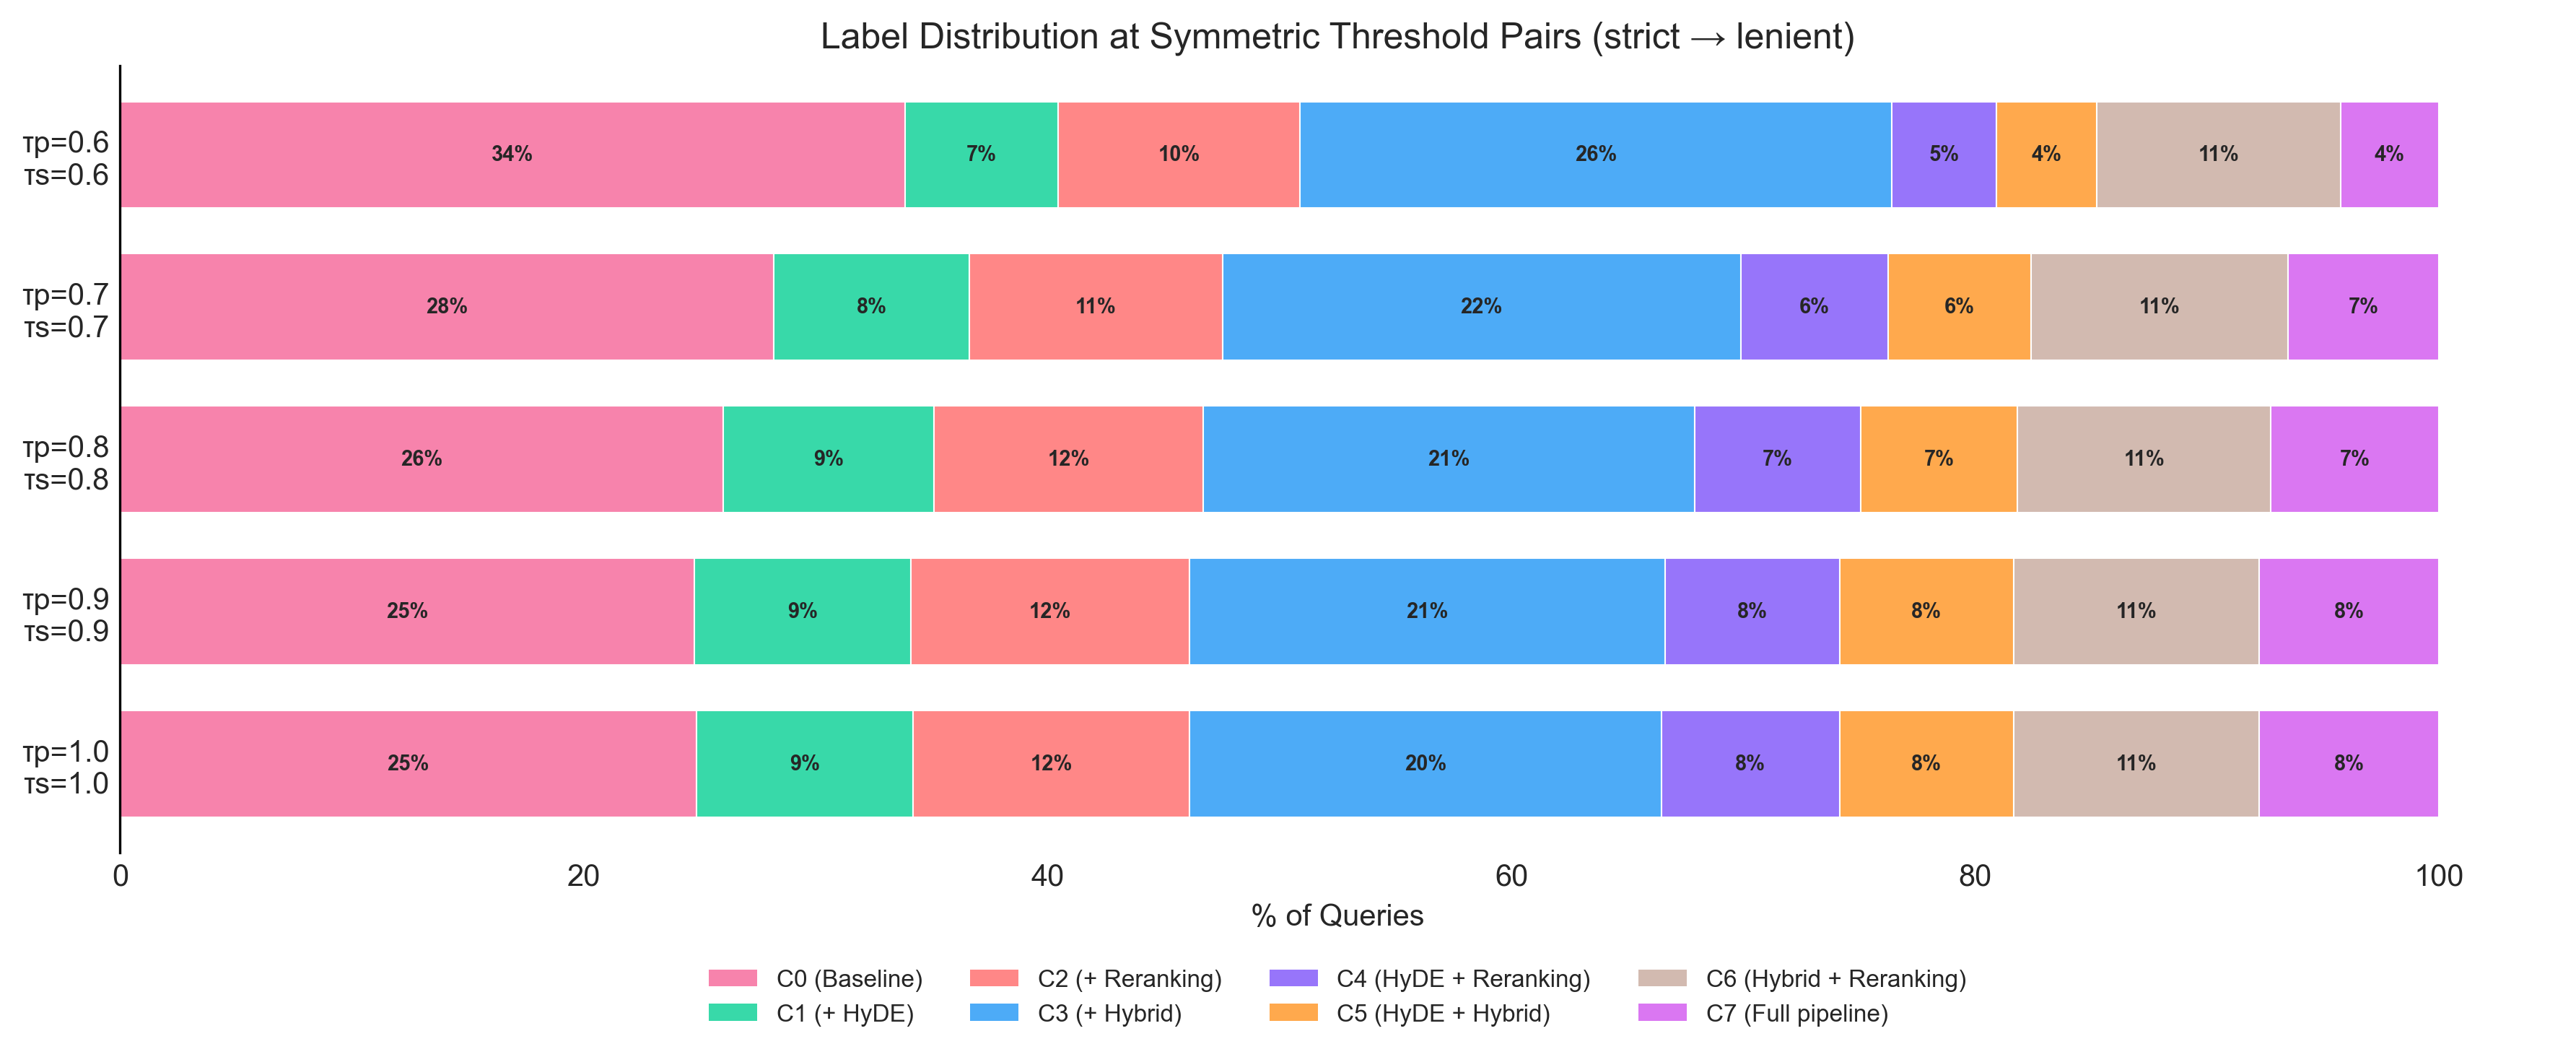
\includegraphics[width=0.95\textwidth]{threshold_label_shift.png}
    \caption{Label distribution at symmetric threshold pairs}
    \label{fig:threshold-label-shift}
    % Source: hotpot/5-label/output/plots/threshold_label_shift.png
\end{figure}


\subsection{Oracle Analysis}
\label{subsec:oracle-analysis}

The oracle router (Equation~\ref{eq:oracle}) selects the cheapest acceptable
configuration with perfect information, defining the theoretical ceiling for any
routing strategy. At default thresholds, 63.0\% of queries (755 of 1{'}200)
have at least one acceptable configuration. these form the
\emph{routable set}. The remaining 37.0\% (445~queries) fail under all
eight configurations; no routing strategy can help them.

On the routable set the oracle achieves a mean energy of
511~J per query versus 1{'}786~J for always-C7: a
\textbf{71\% energy savings ceiling}. 64\% of routable labels go to C0 or C3
(318~J and 324~J respectively). Non-routable queries default to~C0 (318~J),
yielding a combined strategy of
440~J per query (\textbf{75\% savings}).

Queries decompose into three groups:
\begin{itemize}
      \item \emph{Config-diverse} queries (53.0\%) have 1--7 passing configurations at different energy levels; routing adds value.
      \item \emph{All-pass} queries (10\%) pass under every configuration; routing them to~C0 saves the maximum energy.
      \item \emph{Non-routable} queries (37.0\%) fail under every configuration; defaulting to~C0 minimises energy waste.
\end{itemize}

\begin{figure}[h!]
    \centering
    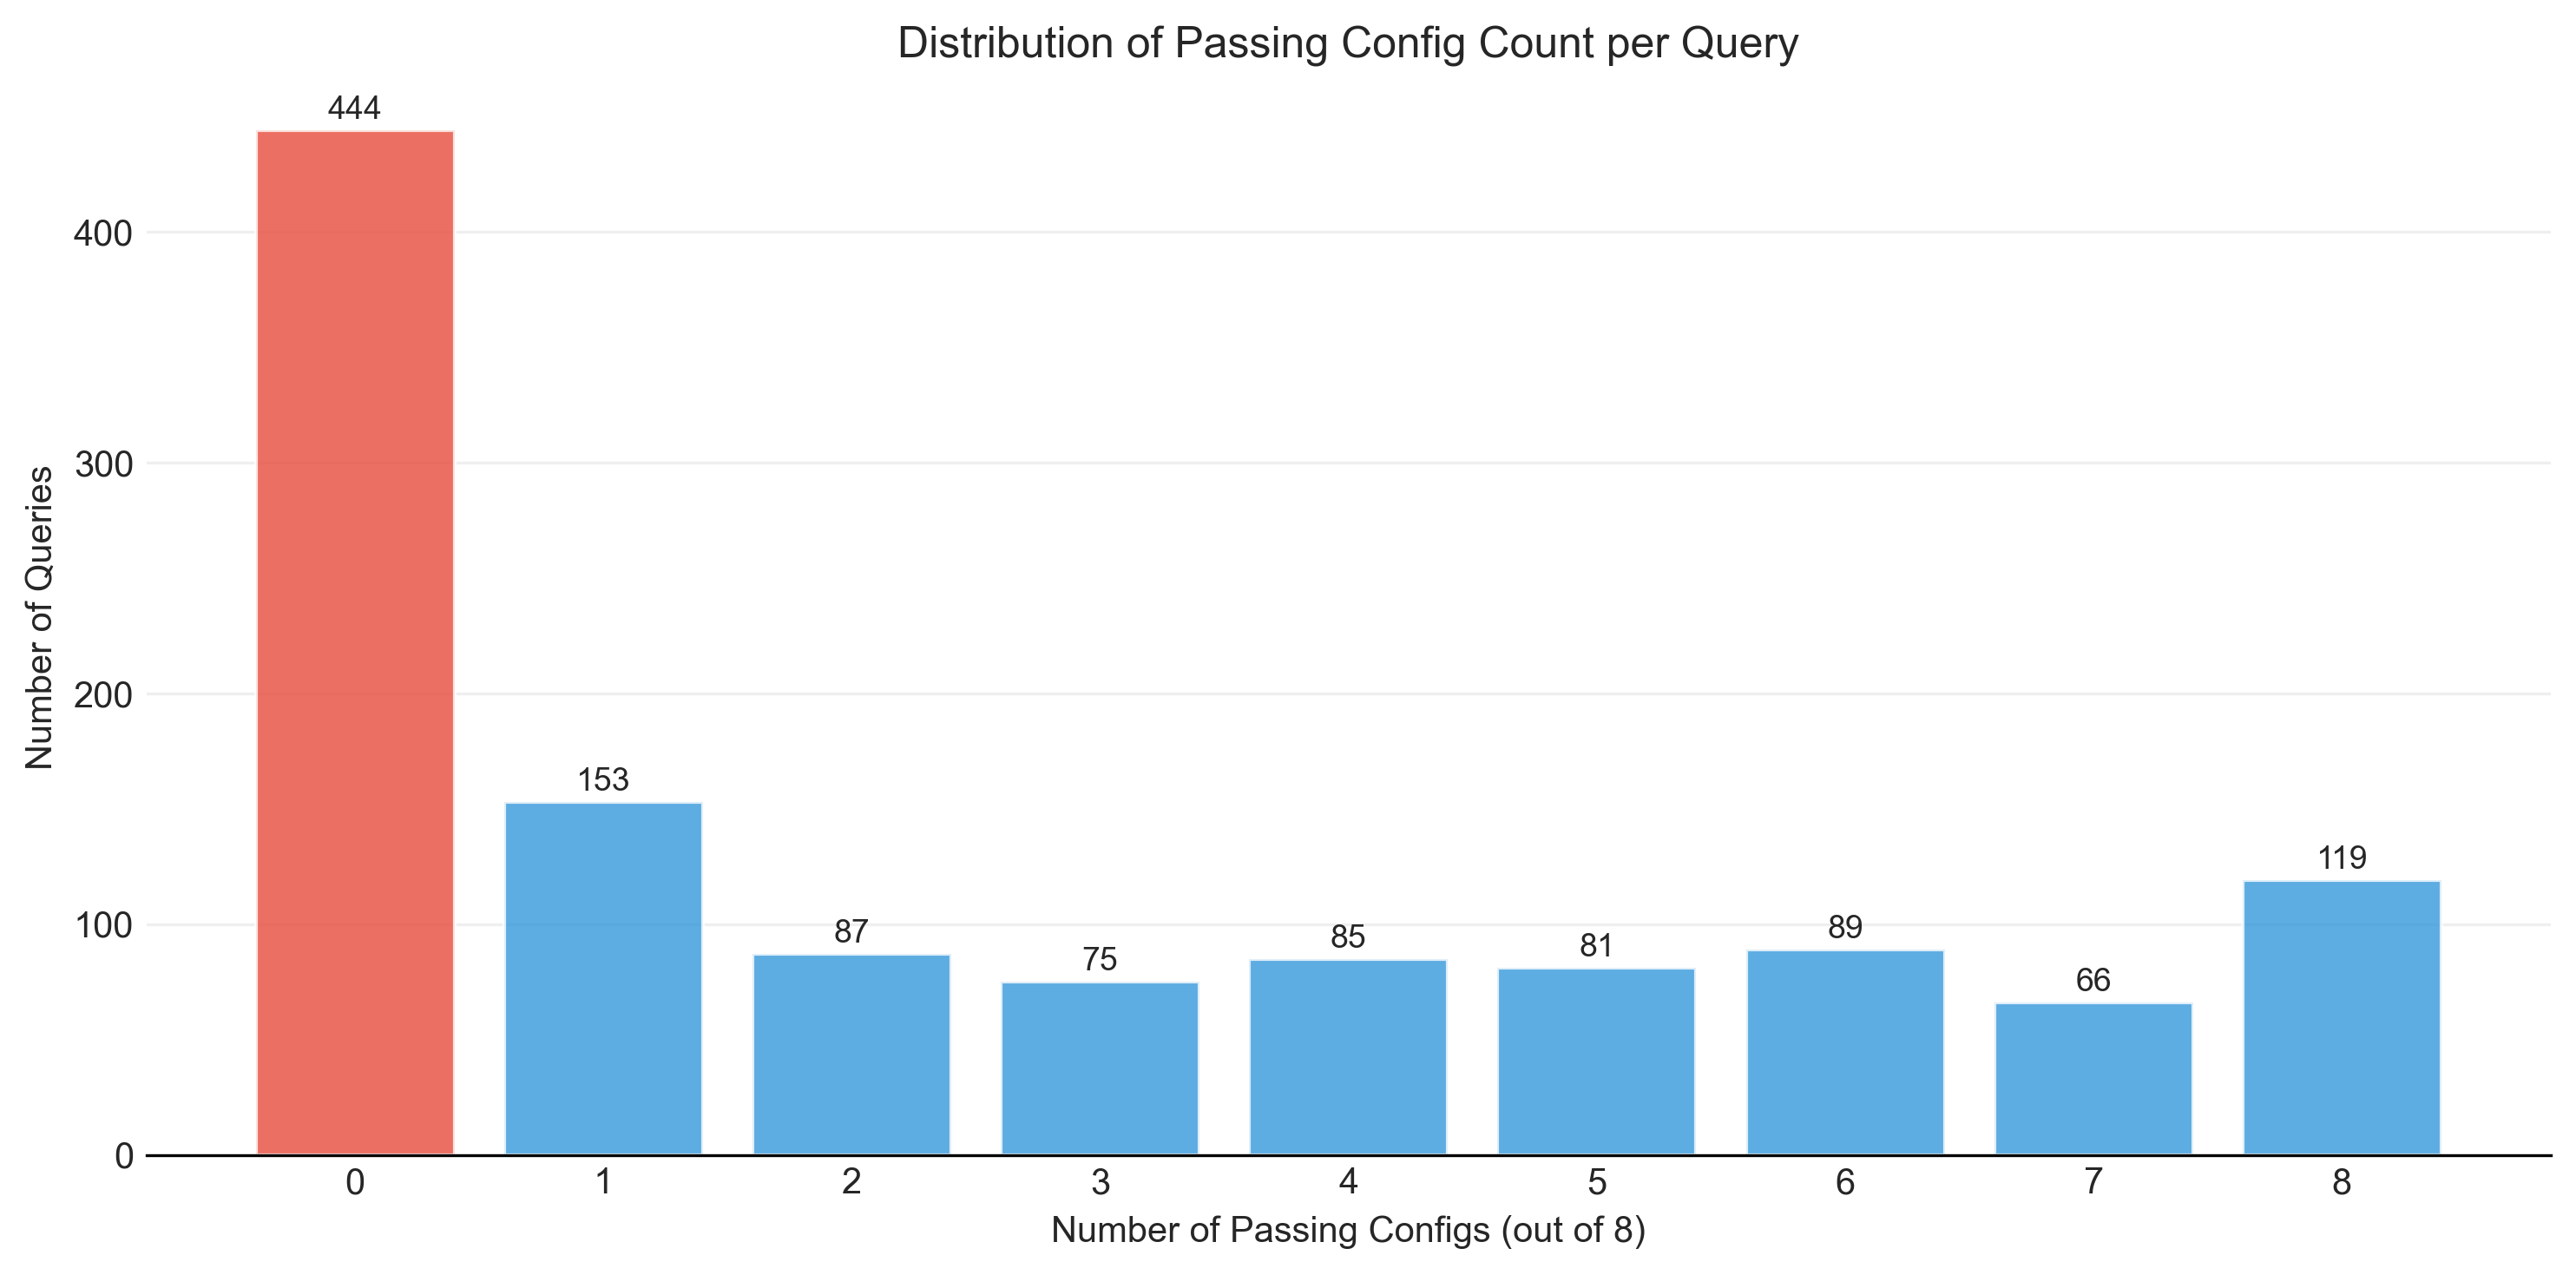
\includegraphics[width=0.85\textwidth]{passing_configs_distribution.png}
    \caption{Distribution of passing configurations per query}
    \label{fig:passing-configs-dist}
    % Source: hotpot/5-label/output/plots/passing_configs_distribution.png
\end{figure}

\paragraph{Scope reduction.}
Given HyDE's negative aggregate quality effect at 5.3$\times$ the energy cost,
a rational deployment default is HyDE-off. The remaining routing problem
operates over four configurations: C0 (baseline), C2 (reranking), C3 (hybrid),
and C6 (hybrid + reranking). This reduces the problem from 8-class to 4-class.
Among passable queries, 89 (11.8\%) have a HyDE configuration as cheapest
acceptable, so the 4-class reduction sacrifices a small fraction of oracle
savings in exchange for halving the label space.

\begin{figure}[h!]
    \centering
    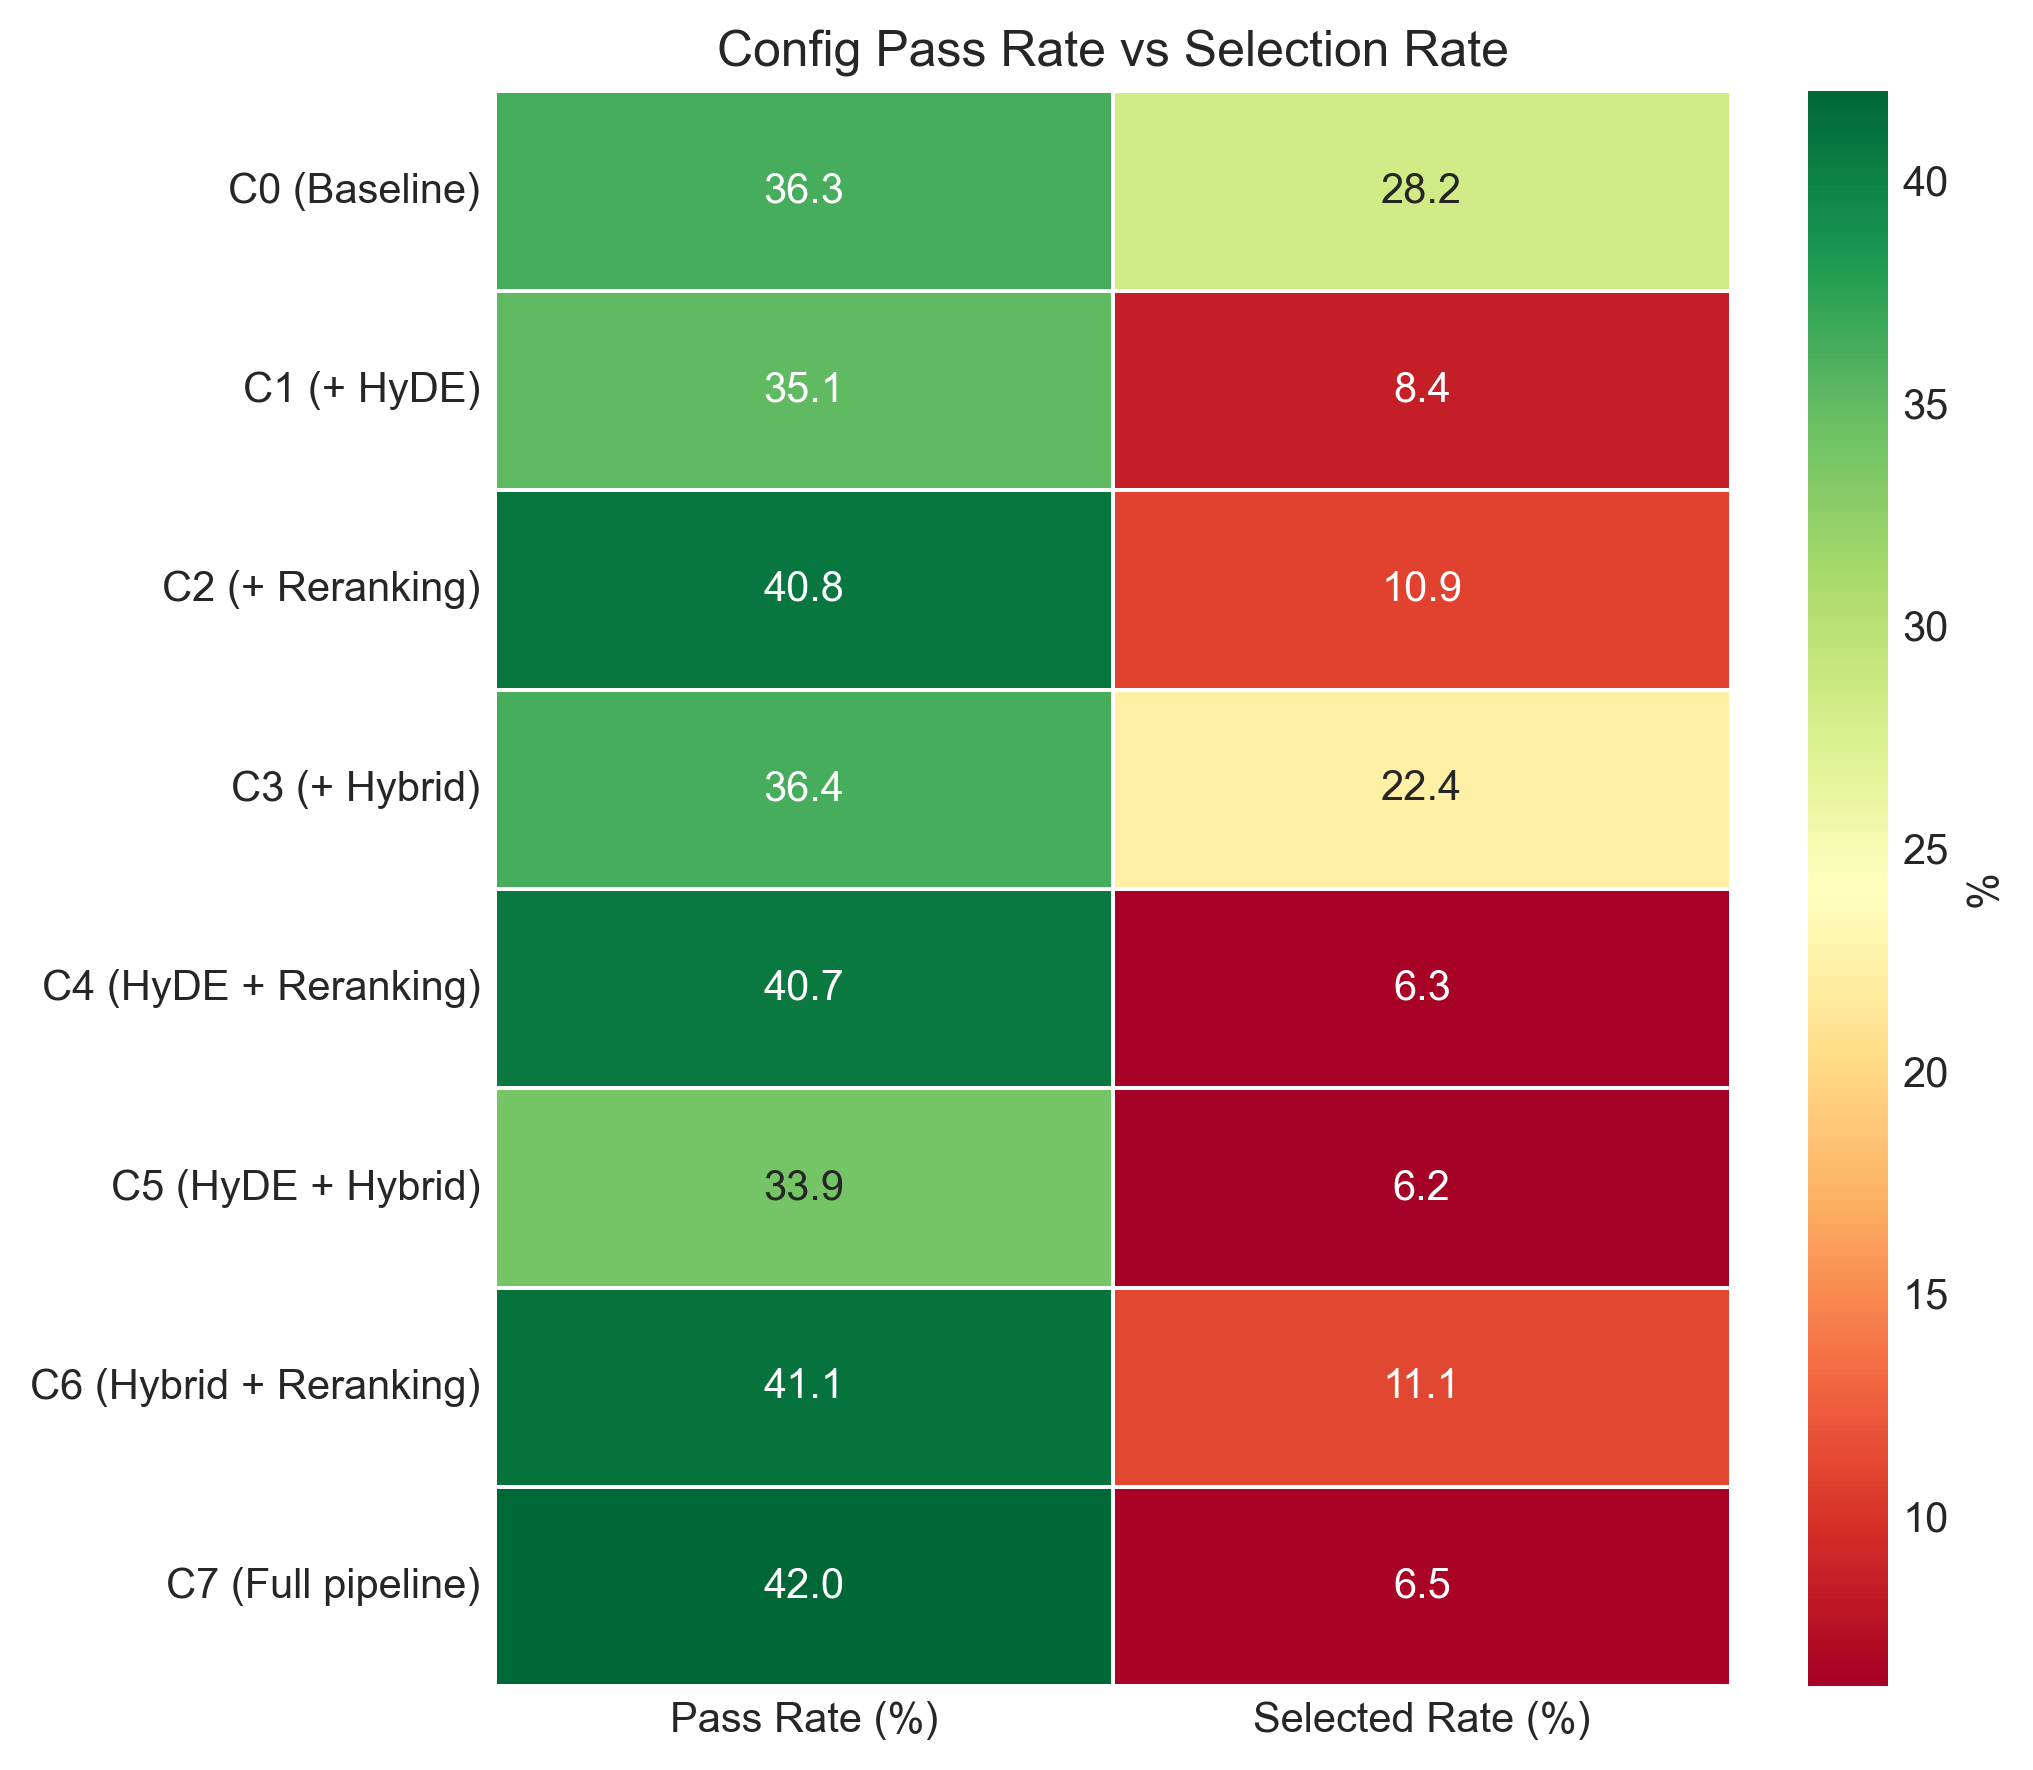
\includegraphics[width=0.75\textwidth]{pass_vs_select_rate.png}
    \caption{Per-configuration pass rate versus oracle selection rate.}
    \label{fig:pass-vs-select}
    % Source: hotpot/5-label/output/plots/pass_vs_select_rate.png
\end{figure}
%All configurations pass at similar rates (33--42\%), but the oracle 
% concentrates selections on C0 and C3 due to their
% lower energy cost. HyDE configurations (C1, C4, C5) are
% selected at 6--8\% despite passing at 33--41\%.


\subsection{Feature Signal Analysis}
\label{subsec:features-signal}

Since the goal is to evaluate whether routing is possible before pipeline execution, only features computable
from the query text and the pre-existing embedding index are used. We
extract 23~pre-execution features in three groups (Table~\ref{tab:query-features}):
Group~A (11 text/rule-based features, $<$1~ms), Group~B (7 NLP features via
spaCy, 1--5~ms), and Group~C (5 embedding-based features that reuse the
retrieval embedding at zero marginal cost).

\begin{table}[h!]
\centering
\small
\begin{tabular}{l c l r}
\hline
\textbf{Feature} & \textbf{Group} & \textbf{Type} & \textbf{Cost} \\
\hline
q\_len\_tokens, q\_len\_chars       & A & numeric   & $<$1\,ms \\
num\_sentences                      & A & numeric   & $<$1\,ms \\
q\_qword                            & A & categorical & $<$1\,ms \\
q\_is\_definition, q\_is\_list      & A & boolean   & $<$1\,ms \\
q\_has\_logical\_operator            & A & boolean   & $<$1\,ms \\
has\_math, has\_code                 & A & boolean   & $<$1\,ms \\
constraint\_count, reasoning\_marker & A & numeric   & $<$1\,ms \\
\hline
q\_ner\_count, q\_ner\_type\_diversity & B & numeric & $<$5\,ms \\
q\_has\_date\_entity, q\_has\_number   & B & boolean & $<$5\,ms \\
q\_multi\_entity                       & B & boolean & $<$5\,ms \\
q\_np\_count, q\_content\_word\_ratio  & B & numeric & $<$5\,ms \\
\hline
q\_emb\_norm                              & C & numeric     & -- \\
q\_emb\_top1\_sim, q\_emb\_top2\_sim      & C & numeric     & -- \\
q\_emb\_sim\_gap                          & C & numeric     & -- \\
q\_sem\_cluster\_id                       & C & categorical & -- \\
\hline
\end{tabular}
\caption{Pre-execution query features}
\label{tab:query-features}
\end{table}
%Group~A requires string operations only,Group~B requires spaCy NLP, Group~C reuses the retrieval embedding.

\paragraph{Signal strength.}
Before building a router, we test whether individual features discriminate among
oracle labels.  Chi-square tests on the nine boolean features find only two
statistically significant associations ($p < 0.05$):
\texttt{q\_has\_logical\_operator} (Cramér's $V = 0.152$, $p < 0.001$) and
\texttt{q\_has\_date\_entity} ($V = 0.114$, $p = 0.030$).  Kruskal--Wallis
tests on the twelve numeric features identify token count
($\eta^2 = 0.013$, $p = 0.002$) and character length
($\eta^2 = 0.010$, $p = 0.009$) as the strongest discriminators; all effect
sizes remain below $\eta^2 = 0.02$, conventionally negligible.
Figure~\ref{fig:top-discriminative-boxplots} confirms this visually: the six
most discriminative features show heavily overlapping distributions across
labels, with only slight median shifts (e.g.\ queries labelled C6 tend 1--2
tokens longer).

A multivariate check via cross-validated gradient-boosted regression on all
21~features yields $R^2 = {-}0.095$ for factual correctness and
$R^2 = {-}0.115$ for faithfulness---both worse than predicting the dataset mean.
Statistically, pre-execution features cannot predict raw quality scores.

However, the routing task is not score prediction.  The router classifies which
pre-computed label a query receives: it need not estimate the score itself, only
whether the cheapest acceptable configuration differs across queries.  Binary
classification of pre-computed labels can succeed even when quality regression
fails, provided the label boundaries align with feature-separable regions in the
input space.

\begin{figure}[h!]
    \centering
    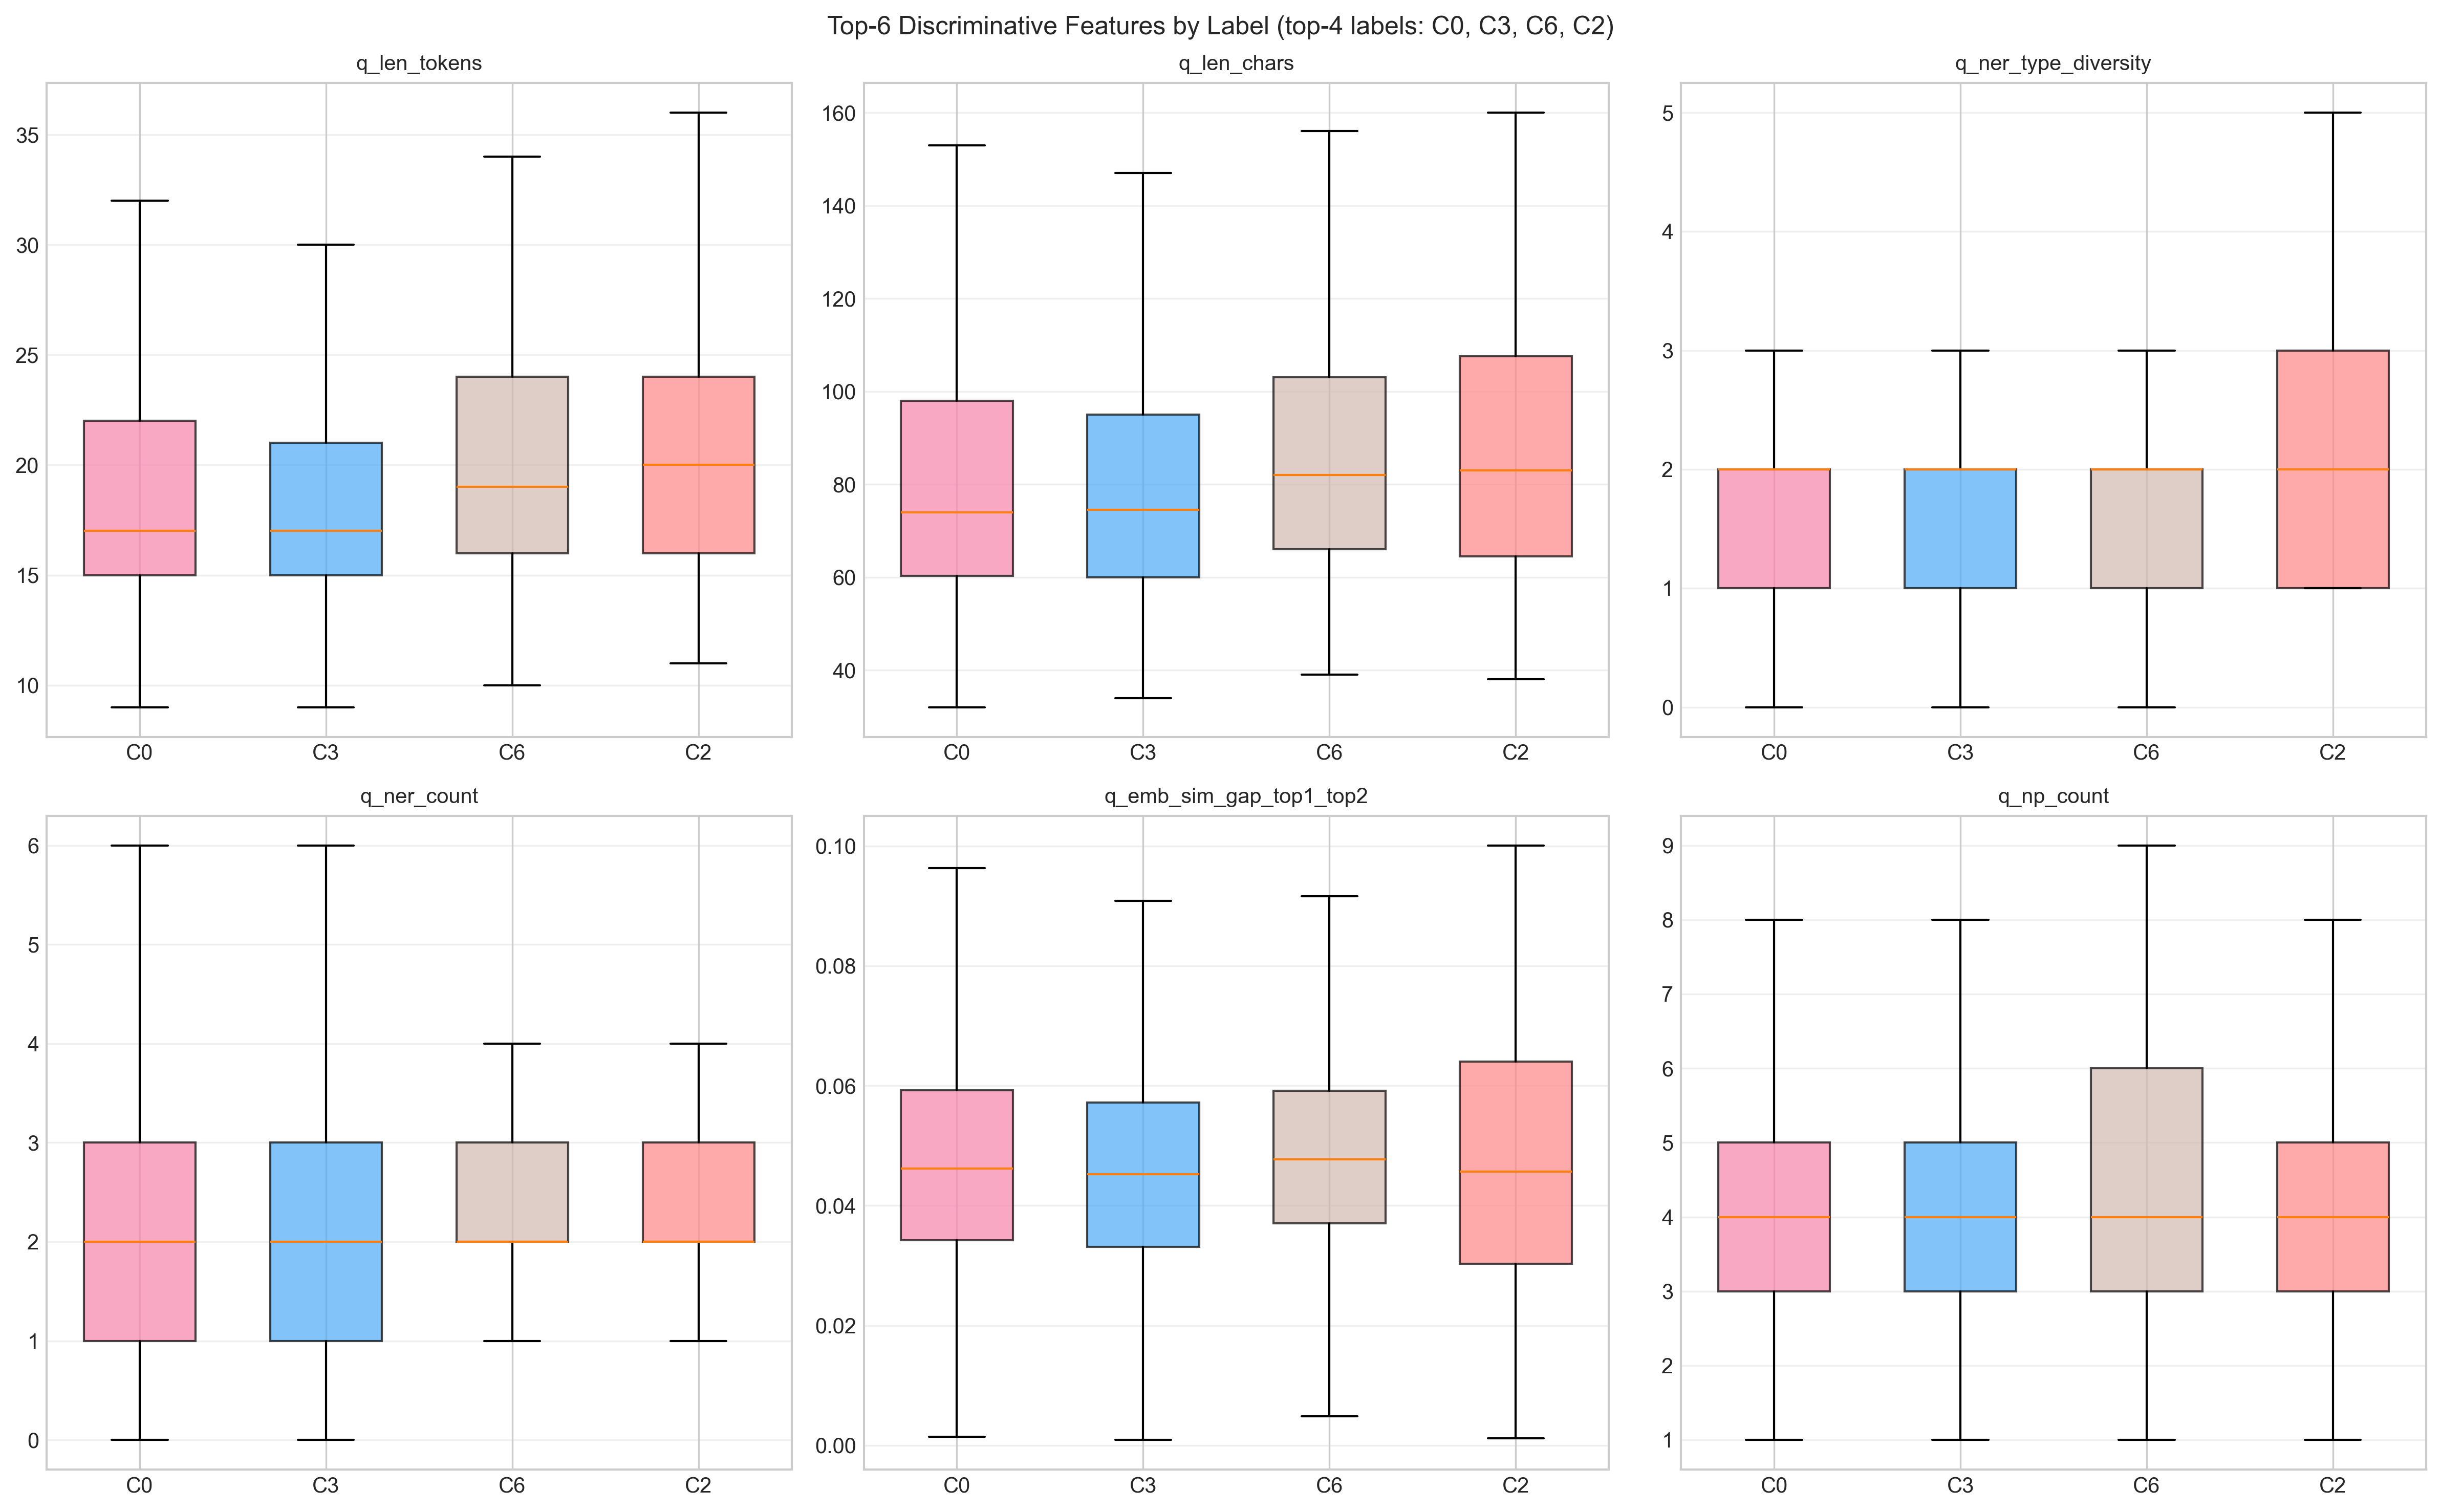
\includegraphics[width=0.95\textwidth]{top_discriminative_boxplots.png}
    \caption{Top-6 discriminative features by oracle label}
    \label{fig:top-discriminative-boxplots}
    % Source: hotpot/5-label/output/plots/top_discriminative_boxplots.png
\end{figure}

\paragraph{Cluster structure.}
To test whether queries group into routing-relevant regions, we apply $k$-means
clustering on all 21~standardised features.  Silhouette analysis over
$k \in \{3, \ldots, 7\}$ selects $k = 7$.  Profiling each cluster by its
highest-mean-FC configuration reveals a two-regime structure: three clusters
(41\% of queries) favour C6 at $\sim$430\,J per query, while three others
(58\%) favour C7 at $\sim$1{'}750\,J.  One small cluster ($n = 4$) favours C3.
The energy gap between regimes is 4$\times$, indicating that cluster membership
carries a routing-relevant signal even though individual features do not.


\subsection{System Constraints}
\label{subsec:integration-constraints}

The router is implemented as a pre-pipeline gate.  As part of this work, we
extended the CITI KMS orchestrator with a per-request configuration API
(Section~\ref{subsec:baseline-config}): the router intercepts the query,
extracts features, predicts a configuration and passes it to the orchestrator.
No modification to the pipeline stages themselves is required.  Total feature
extraction overhead (1--5\,ms for spaCy; embedding features are free) is
negligible compared to mean pipeline execution times, which range from
982\,ms (C0) to 6{'}153\,ms (C7). We estimate the router's energy cost at
$\sim$0.08\,J per query (CPU at $\sim$15\,W effective load $\times$ 5\,ms),
four orders of magnitude below the cheapest pipeline (318\,J).

Two constraints bound the router design:
\begin{enumerate}
    \item \textbf{Latency}: the routing decision should add at most tens of
          milliseconds---within 1--1O\% of the cheapest pipeline
          configuration.
    \item \textbf{Simplicity}: the model must be lightweight (no GPU),
    interpretable where possible and, in this specific case, trainable on $\sim$755~queries. 
\end{enumerate}

\paragraph{Key Idea.}
The oracle ceiling (Section~\ref{subsec:oracle-analysis}) sets the upper bound;
64\% of routable labels go to the two cheapest configurations.
Pre-execution features carry near-zero quality signal ($R^2 \approx 0$),
but label classification is a different task than score prediction.
HyDE's negative quality effect reduces the problem from eight to four
configurations. Chapter~\ref{sec:strategies} evaluates whether practical
routers can capture a meaningful fraction of this ceiling.


\newpage
\section{Routing Strategies}
\label{sec:strategies}

% Chapter purpose: Systematic investigation revealing a structural ceiling for
% pre-execution routing on the no-HyDE config space {C0, C2, C3, C6}.
% Narrative: survey (S1–S5, nothing beats C0) → explorations (E1–E3) →
% ceiling analysis (the contribution).
% Data: hotpot/7-routing/ (exploratory), hotpot/8-routing/ (controlled).


\subsection{Experimental Setup}
\label{subsec:routing-setup}

Previously we formulated the routing decision, constructed
oracle label  and assessed the pre-execution signal.  Now, we
evaluate whether learned routing strategies can exploit that signal
beyond a static baseline. The objective remains:
%
\begin{quote}
Given a query~$q$ with pre-execution features
$\mathbf{x} \in \mathbb{R}^d$, select the configuration
$\hat{c}(q) \in \mathcal{C} = \{\text{C0, C2, C3, C6}\}$
that minimises energy while satisfying the quality floor.
\end{quote}
%
This uses no information produced by the pipeline itself. The 
configuration space $\mathcal{C}$ is reduced to non-HyDE configurations.

\begin{figure}[h!]
\centering
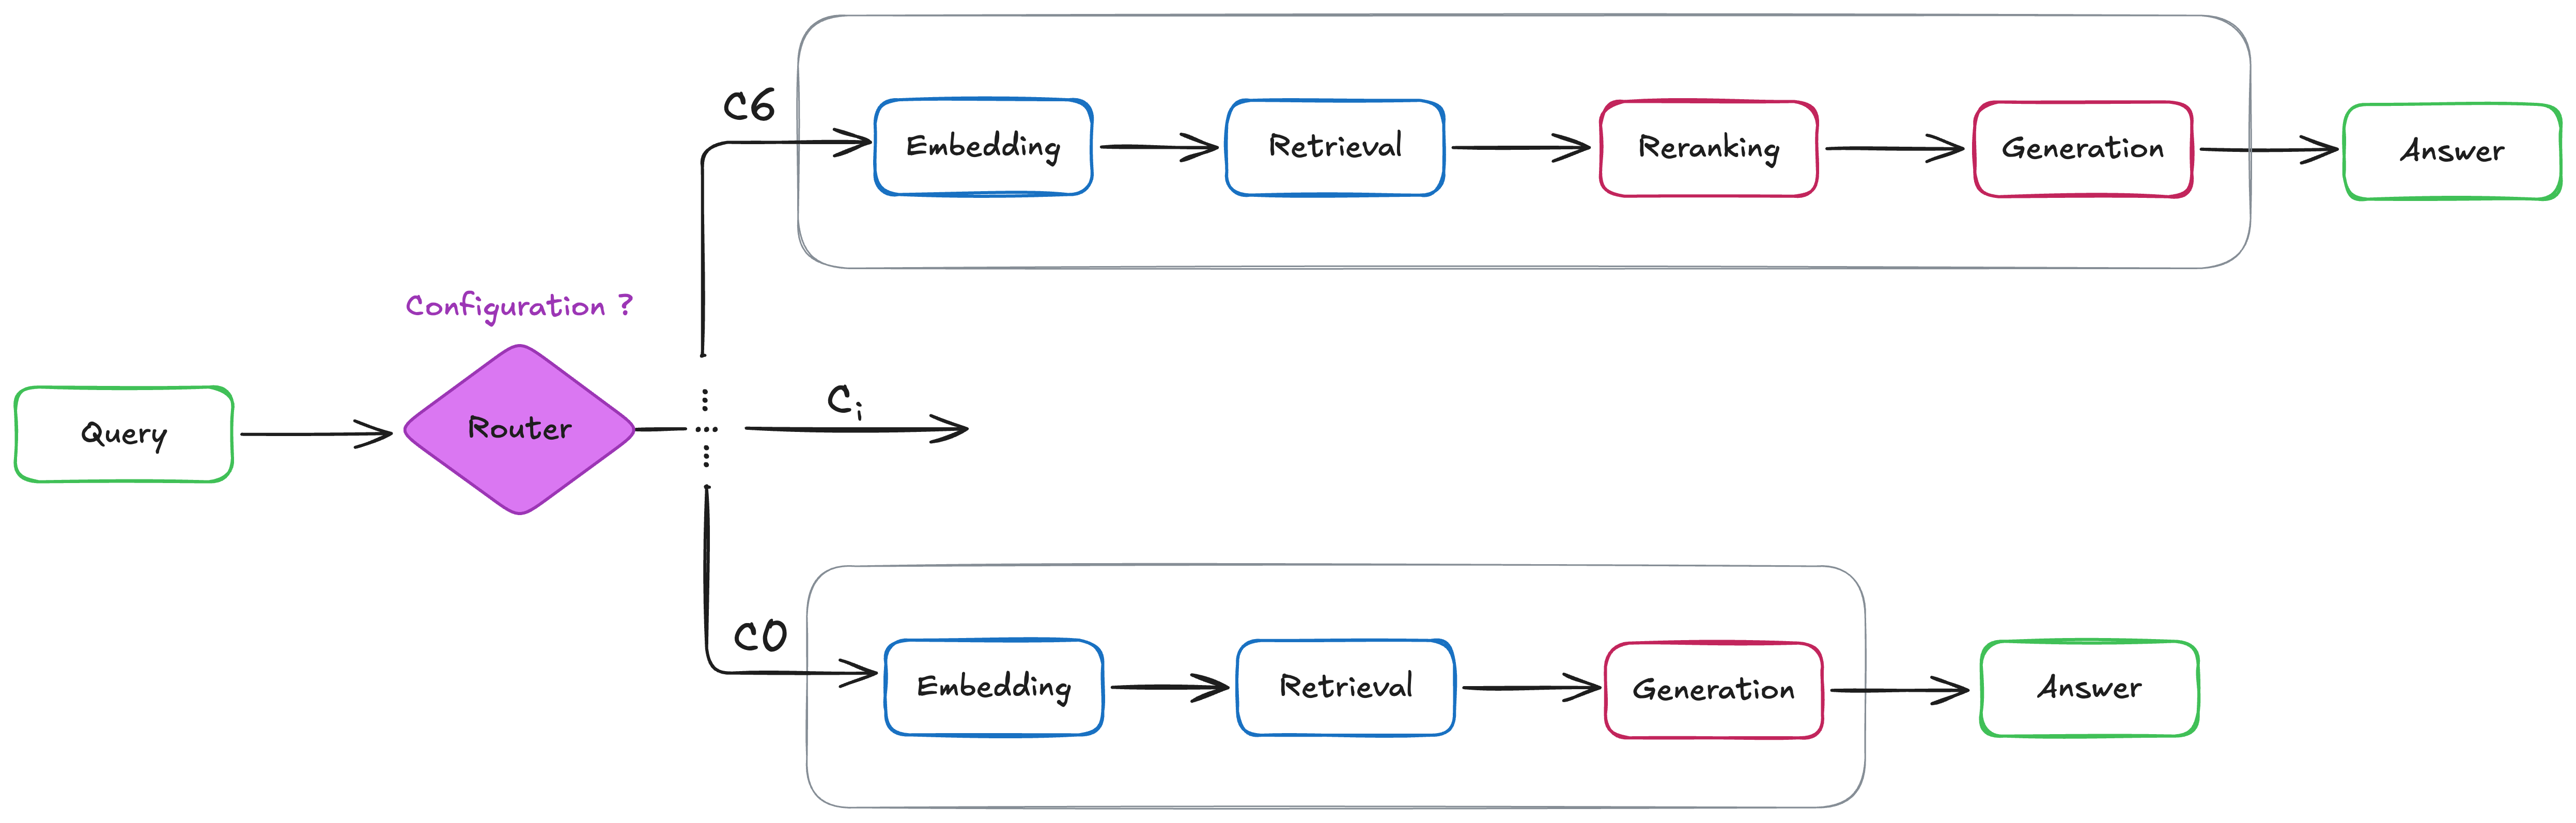
\includegraphics[width=0.85\textwidth]{router.png}
\caption{Router flow illustration}
\label{fig:router-flow}
\end{figure}

\paragraph{Evaluation protocol.}
Let $\mathcal{D} = \{(\mathbf{x}_i, y_i)\}_{i=1}^{N}$ denote the routing
dataset, where $\mathbf{x}_i \in \mathbb{R}^{d}$ is the pre-execution
feature vector and $y_i = \ell(q_i) \in \mathcal{C}$ the oracle label
for query~$i$. Features are query-only meaning that every configuration
sees the same~$\mathbf{x}_i$. The label is config-dependent because $\ell(q)$ 
selects the cheapest configuration that satisfies the quality floor:
encoding both energy and quality information in a single target.

The base dataset contains $N = 1{'}200$ queries
with $d = 23$ features; individual experiments vary~$d$ as noted.
All models are evaluated under 5-fold stratified cross-validation,
stratified on~$y_i$ to preserve class proportions,
with 80/20\% train-test splits. Five metrics measure success:

\begin{itemize}
    \item \textbf{Config accuracy}: the fraction of queries routed to the oracle-optimal configuration. Primary metric.
          $$\text{acc} = \frac{1}{N} \sum_{i=1}^{N}
          \mathbb{1}[\hat{y}_i = y_i]$$
    \item \textbf{Config F1 macro}: the macro-averaged F1 across configuration classes.  Penalises
          models that ignore minority classes.
          $$\text{F1}_{\text{macro}} = \frac{1}{|\mathcal{C}|}
          \sum_{c \in \mathcal{C}} \text{F1}_c$$
    \item \textbf{Pass rate}: the fraction of queries whose routed configuration produces an
          acceptable response ($a = 1$).  Pass rate inflates apparent
          performance because multiple configurations satisfy the same query.
          $$\text{pass} = \frac{1}{N} \sum_{i=1}^{N}a(q_i, \hat{y}_i)$$
    \item \textbf{Mean energy/token}: the average energy/token per query under the routed policy.
          $$\bar{E} = \frac{1}{N} \sum_{i=1}^{N} E(q_i, \hat{y}_i)$$
    \item \textbf{Mean ROC AUC} measures a model's average ability to distinguish
    between classes across multiple folds. 
\end{itemize}

\paragraph{Baselines.}
The simplest reference is a \emph{configuration baseline}: apply the same
configuration to every query without any routing.
%$ \hat{c}(q) = c_j,\; \forall q$.
There are four such baselines, one per configuration in~$\mathcal{C}$.
The \emph{oracle} which assigns each query to its most energy-efficient configuration,
$\hat{c}(q) = y_i$. The table below reports the
results.  Among them, C0 achieves the highest accuracy
(0.382) because C0 is the most frequent oracle label.  Any learned router
must exceed this threshold to justify its complexity.
Figure~\ref{fig:baseline-energy} illustrates the energy cost between the baselines.

\begin{table}[h!]
\centering
\begin{tabular}{l r r r r r}
\hline
\textbf{Baseline} & \textbf{Accuracy} & \textbf{F1 macro}  & \textbf{Pass rate} & \textbf{Energy (J)} \\
\hline
Oracle  & 1.000 & 1.000   & 0.555 & 341 \\
C0      & 0.382 & 0.138   & 0.318 & 318 \\
C3      & 0.318 & 0.121   & 0.323 & 324 \\
C2      & 0.153 & 0.066   & 0.363 & 424 \\
C6      & 0.148 & 0.064   & 0.362 & 435 \\
\hline
\end{tabular}
\caption{Configuration baselines and oracle.}
\label{tab:baselines}
\end{table}

\begin{figure}[h!]
\centering
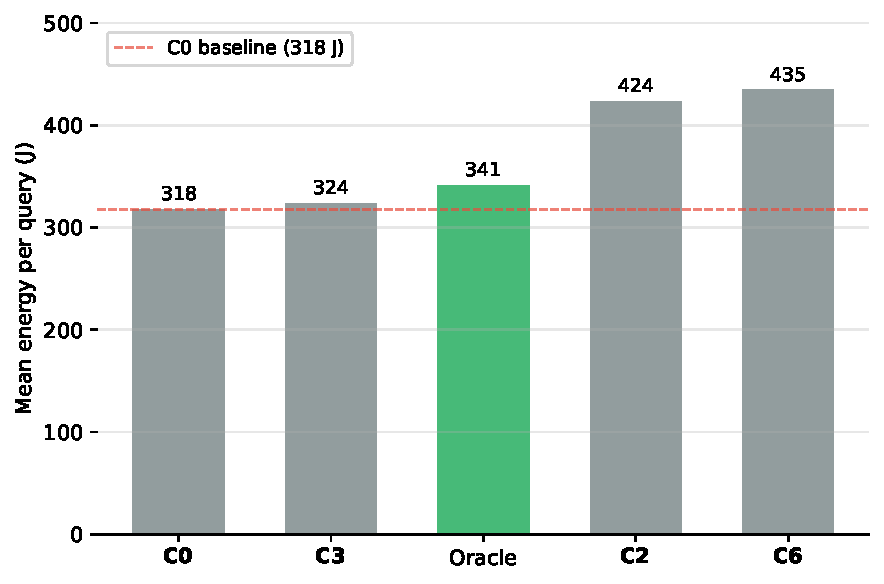
\includegraphics[width=0.7\textwidth]{fig_baseline_energy.pdf}
\caption{Mean energy per query across configuration baselines.}
\label{fig:baseline-energy}
\end{figure}

\paragraph{Investigation design.}
The investigation proceeds in two phases:
\begin{enumerate}
    \item \textbf{Strategy survey}
          (Section~\ref{subsec:strategy-survey})
          Five ML framings of the routing task---multiclass
          classification, binary decomposition, pairwise
          preference, selective abstention and utility scoring---are
          evaluated using the same 23~pre-execution features and
          tree-based classifiers.
    \item \textbf{Explorations}
          (Section~\ref{subsec:explorations})
          We fix the best formulation (utility scoring) and probe
          three dimensions: feature selection~(E1), quality-metric
          definition~(E2) and test-architecture~(E3).
\end{enumerate}

Together, the two phases test whether the performance ceiling is signal-limited or model-limited.

% The controlled study spans four dimensions:
% \begin{itemize}
%       \item 3 feature sets (10~top-importance, 23~handcrafted, 23~+~5~C0 retrieval statistics)
%       \item 2 label definitions (fc~+~faithfulness; fc~+~faithfulness~+~sup\_f1)
%       \item 3 model families (tree-based classifiers, MLP with energy-aware loss (Neural network), two-stage cascade)
%       \item 2 decision architectures (flat two-model with independent hybrid and reranking heads 
%       vs.\ two-stage cascade where Stage~1 predicts search type, executes retrieval and 
%       Stage~2 predicts reranking from the retrieved results).
% \end{itemize}



\subsection{Strategy Survey}
\label{subsec:strategy-survey}

We tested five routing formulations
(S1--S5) to find which prediction target can selectively assign
expensive configurations when they help, rather than defaulting to
the cheapest option for every query. All five use the same 23~pre-execution features,
the same evaluation protocol and tree-based classifiers where
applicable. 
% The table below summarises results whereas 
% the paragraphs below trace the logical progression.

\begin{table}[h!]
\centering
\small
\begin{tabular}{c l l l r}
\hline
\textbf{ID} & \textbf{Strategy} & \textbf{Prediction target} & \textbf{Model} & \textbf{Acc} \\
\hline
S1 & Multiclass          & Oracle label (4-class)        & LR / RF / XGB          & 0.297 \\
S2 & Binary decomp.      & Hybrid? + Rerank? (indep.)    & RF (two heads)         & 0.298 \\
S3 & Pairwise pref.      & Config~A $>$ B? (6 pairs)     & RF + voting            & 0.331 \\
S4 & Selective abstention & Oracle label + confidence     & RF + threshold         & ---   \\
S5 & Utility scoring     & $\hat{P}$(pass $\mid$ q, c)   & RF (per-config) + $\lambda$ & 0.395 \\
\hline
\end{tabular}
\caption{Strategy survey results.}
\label{tab:strategy-survey}
\end{table}

\paragraph{S1: Direct multiclass classification.}
The most direct and naïve approach predicts the configuration label among
\{C0, C2, C3, C6\} using logistic regression, random forest and
XGBoost.  The best classifier (XGBoost) reaches the poor config accuracy of
0.297.

\begin{figure}[h!]
\centering
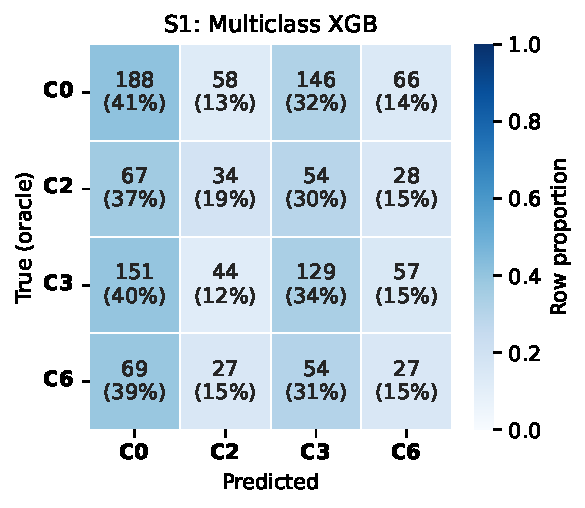
\includegraphics[width=0.55\textwidth]{fig_cm_s1_multiclass.pdf}
\caption{S1 confusion matrix (XGBoost, best classifier).}
\label{fig:cm-s1}
\end{figure}

\paragraph{S2: Binary decomposition.}
To reduce class imbalance, we decompose the 4-class problem into two
independent binary heads: ``needs hybrid search?'' and ``needs
reranking?''  Two random-forest classifiers predict each decision
separately; their outputs combine into a configuration.  Best accuracy
reaches 0.298. The individual heads are too
weak to improve over majority-class prediction and the selection
mechanism has no notion of energy cost
(Figure~\ref{fig:cm-s2}).

\begin{figure}[h!]
\centering
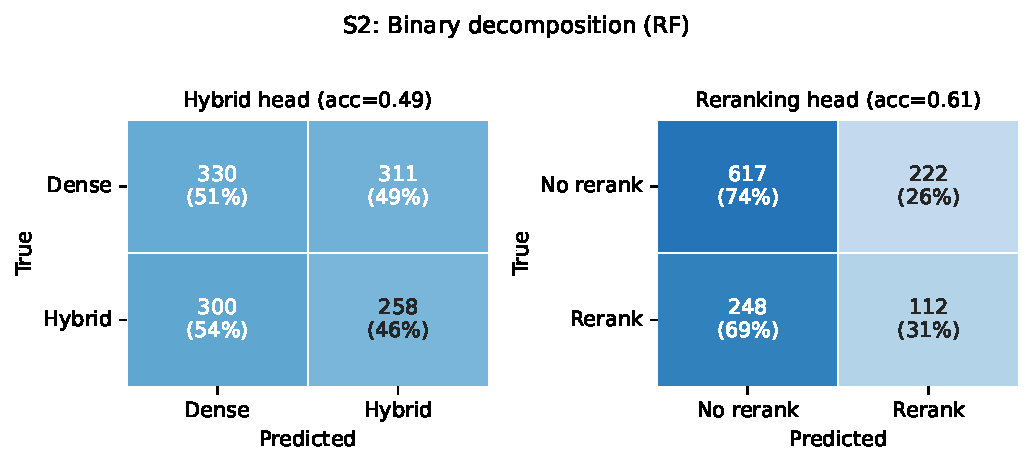
\includegraphics[width=0.75\textwidth]{fig_cm_s2_binary.pdf}
\caption{S2 confusion matrices for the hybrid and reranking binary heads (RF).}
\label{fig:cm-s2}
\end{figure}

\paragraph{S3: Pairwise preference.}
Instead of predicting a single label, we train six pairwise classifiers
(one per configuration pair) and aggregate via Borda voting.  Best
accuracy reaches 0.331.  When individual pairs cannot reliably
distinguish configurations with 2--3~pp quality differences, voting
amplifies noise rather than signal
(Figure~\ref{fig:cm-s3}).

\begin{figure}[h!]
\centering
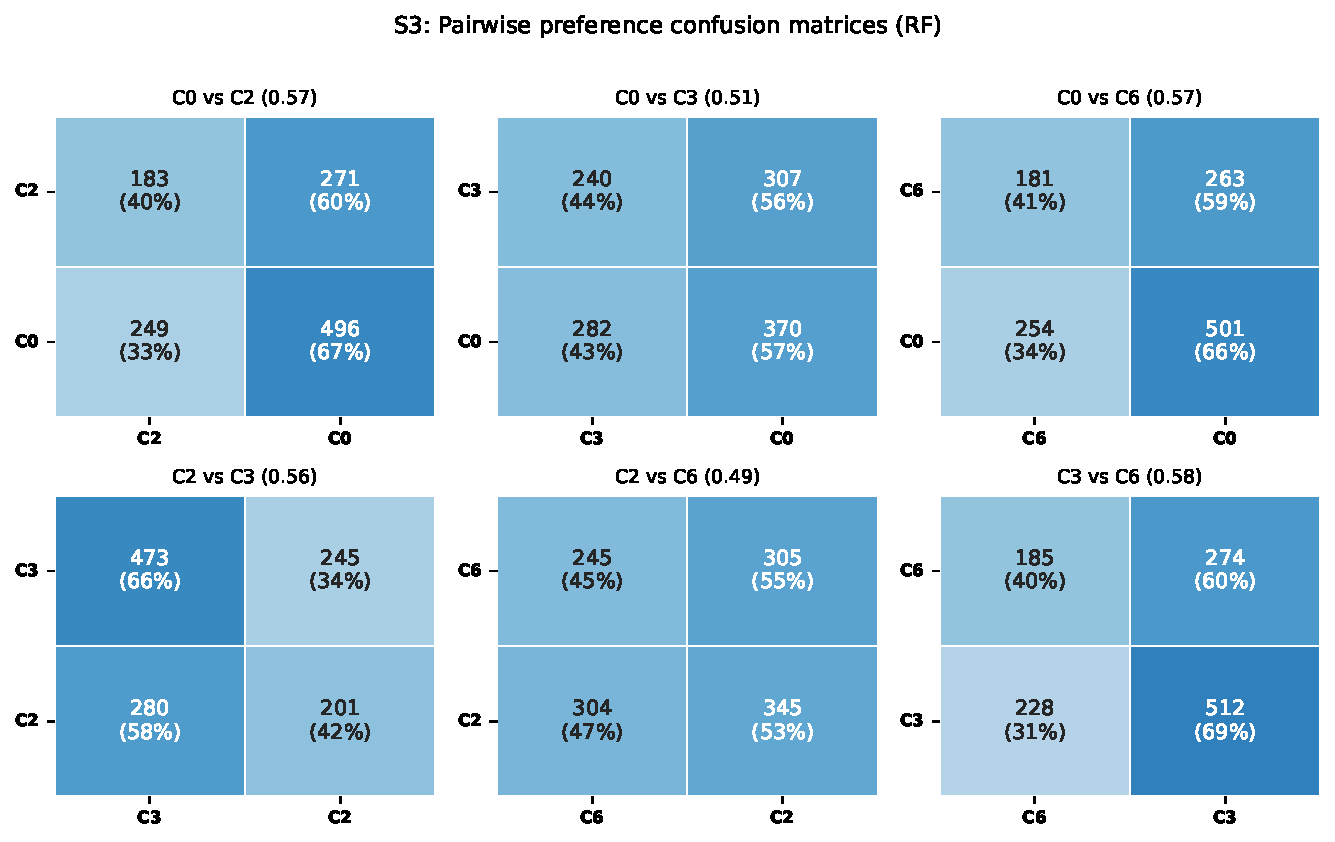
\includegraphics[width=0.85\textwidth]{fig_cm_s3_pairwise.pdf}
\caption{S3 pairwise preference confusion matrices (RF).}
\label{fig:cm-s3}
\end{figure}

\paragraph{S4: Selective abstention.}
We add a confidence threshold: route only when the classifier's
predicted probability exceeds a minimum, otherwise fall back to the
cheapest configuration.  At every threshold that maintains meaningful
routing coverage, 68--90\% of queries fall back to the default.
The classifier is rarely confident because the underlying signal is
weak, making abstention impractical
(Figure~\ref{fig:s4-abstention}).

% \begin{figure}[h!]
% \centering
% \includegraphics[width=0.6\textwidth]{fig_s4_abstention_curve.pdf}
% \caption{S4 abstention rate vs config accuracy ($\lambda = 0.75$, fallback C0).}
% \label{fig:s4-abstention}
% \end{figure}

\subsection{Utility Scoring}
\label{subsec:utility-scoring}

The four previous strategies share two failure modes: direct label
prediction is trapped by class imbalance, and no approach accounts
for energy cost during selection.  Utility scoring addresses both.
Instead of predicting the oracle label, we train a binary classifier
\emph{per configuration} that estimates $\hat{P}(\text{pass} \mid q, c)$
---the probability that query~$q$ produces an acceptable response under
configuration~$c$.  Two separate classifiers predict the search-type and
reranking decisions independently.  Configuration selection uses:
%
\begin{equation}
c^*(q) = \arg\max_{c \in \mathcal{C}} \;\;
    \hat{P}(\text{pass} \mid q, c) \;-\; \lambda \cdot
    \widetilde{E}(c)
\label{eq:utility}
\end{equation}
%
where $\widetilde{E}(c)$ is the min-max normalised energy cost of
configuration~$c$ and $\lambda$ controls the energy--quality trade-off.
Ties are broken in favour of the cheaper configuration.  This framework
decouples quality estimation from configuration selection: the classifiers
learn pass probabilities without knowing the energy landscape, while
the utility function injects energy awareness at inference time.

\begin{figure}[h!]
\centering
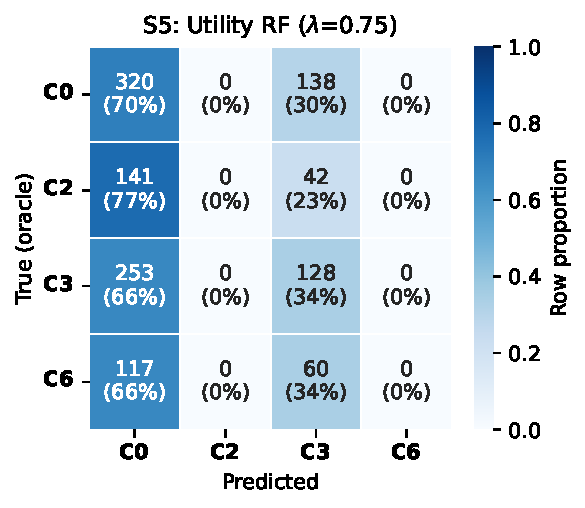
\includegraphics[width=0.55\textwidth]{fig_cm_s5_utility.pdf}
\caption{S5 confusion matrix (RF, $\lambda = 0.75$).}
\label{fig:cm-s5}
\end{figure}

\paragraph{Survey outcome.}
Utility scoring is the only formulation that avoids the majority-class
trap and introduces energy awareness.  At $\lambda = 1.50$, it exceeds
Static~C0 for the first time, on a minimal note though
(0.395 in the explorations below).  We also tested single-head MLPs
with an energy-aware loss ($\mathcal{L} = \text{BCE} + \alpha \cdot
\delta \cdot \text{sigmoid}(\text{logit})$), but 2{'}000~training
samples proved insufficient: the best variant reached 0.383, matching
the tree baselines without improving on~S5.

Table~\ref{tab:all-strategies} consolidates the best policy from each
strategy alongside the baselines.  All approaches cluster in a narrow
band: config accuracy does not exceed 40\%.

\begin{table}[h!]
\centering
\small
\begin{tabular}{l l r r r r}
\hline
\textbf{Strategy} & \textbf{Best policy} & \textbf{Acc} & \textbf{F1 macro} & \textbf{Pass rate} & \textbf{Energy (J)} \\
\hline
Oracle                 & ---                      & 1.000 & 1.000 & 0.555 & 341 \\
\hline
S5: Utility scoring    & RF $\lambda$=1.50        & 0.395 & 0.189 & 0.328 & 318 \\
MLP (energy loss)      & MLP $\lambda$=1.50       & 0.383 & 0.165 & 0.318 & 317 \\
\hline
Static C0              & ---                      & 0.382 & 0.138 & 0.318 & 318 \\
\hline
S3: Pairwise pref.     & RF + voting              & 0.331 & 0.149 & 0.323 & 335 \\
S2: Binary decomp.     & RF (two heads)           & 0.298 & 0.103 & 0.316 & 361 \\
S1: Multiclass         & XGB                      & 0.297 & 0.131 & 0.325 & 340 \\
\hline
\end{tabular}
\caption{Consolidated strategy results (best policy per approach).}
\label{tab:all-strategies}
\end{table}

\paragraph{Lambda dominance.}
Across all experiments, the best results appear at $\lambda = 1.25$--$1.50$.
Without the energy penalty ($\lambda = 0$), config accuracy drops to
0.28--0.35 as models route queries to expensive configurations.
The energy weight $\lambda$ is more impactful than the choice of
classifier or formulation.  High~$\lambda$ enforces cheap defaults
unless the quality signal is strong, which amounts to a soft version
of Static~C0.  Figure~\ref{fig:lambda-sweep} shows the monotonic
relationship: all three classifiers start 8--10~pp below Static~C0 at
$\lambda = 0$ and converge toward it as $\lambda$ increases.  Only RF
at $\lambda \geq 1.25$ crosses the baseline.

\begin{figure}[h!]
\centering
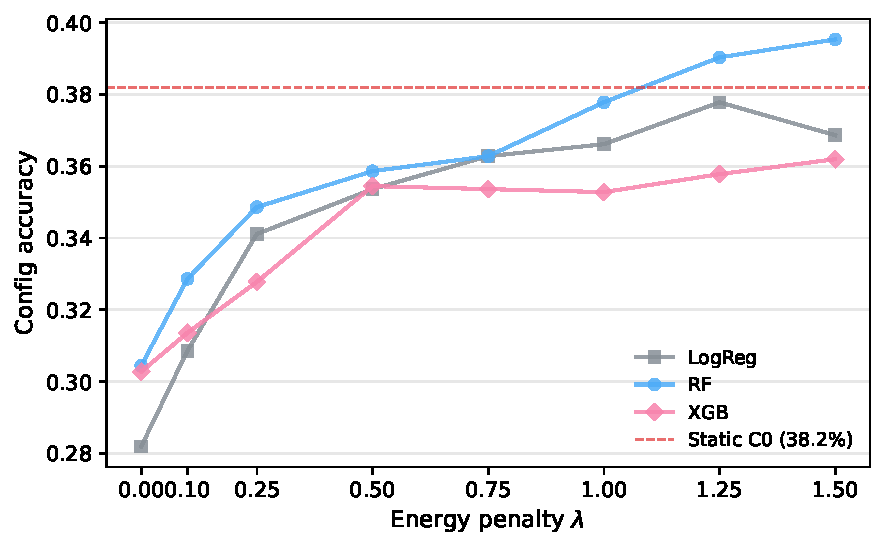
\includegraphics[width=0.7\textwidth]{fig_lambda_sweep.pdf}
\caption{Config accuracy versus energy penalty $\lambda$}
\label{fig:lambda-sweep}
\end{figure}

\subsection{Routing Explorations}
\label{subsec:explorations}

Given that utility scoring is the most promising formulation that exceeds
Static~C0, we explored some of its boundaries.  Three experiments probe
different dimensions of the approach: which features carry routing
signal~(E1), which quality-metric definition produces learnable
labels~(E2) and whether a two-stage architecture can access
post-retrieval information~(E3).


\subsubsection{Feature Selection (E1)}
\label{subsubsec:feature-importance}

We select the ten features with the highest importance scores from a
preliminary correlation analysis and compare per-model performance
against full 23-feature set.  The goal is to determine whether
the routing signal is concentrated or distributed.

\begin{figure}[h!]
\centering
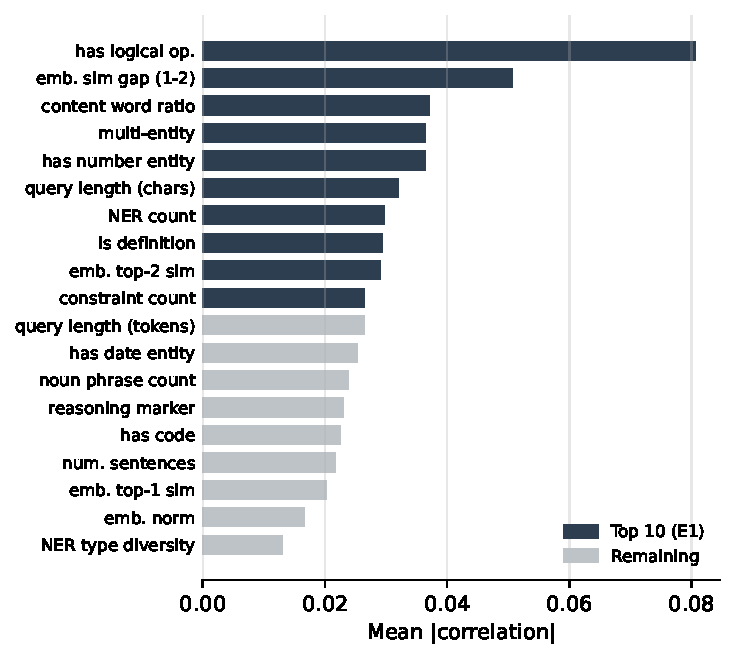
\includegraphics[width=0.6\textwidth]{fig_e1_feature_importance.pdf}
\caption{Top-10 feature importance scores.}
\label{fig:e1-importance}
\end{figure}

It turns out that the top four are: presence of a logical operator,
embedding similarity gap between the two nearest semantic clusters,
content-word ratio and multi-entity flag.
Structural query properties and embedding-derived difficulty signals
carry the most routing-relevant information for the HotPotQA dataset.

\begin{figure}[h!]
\centering
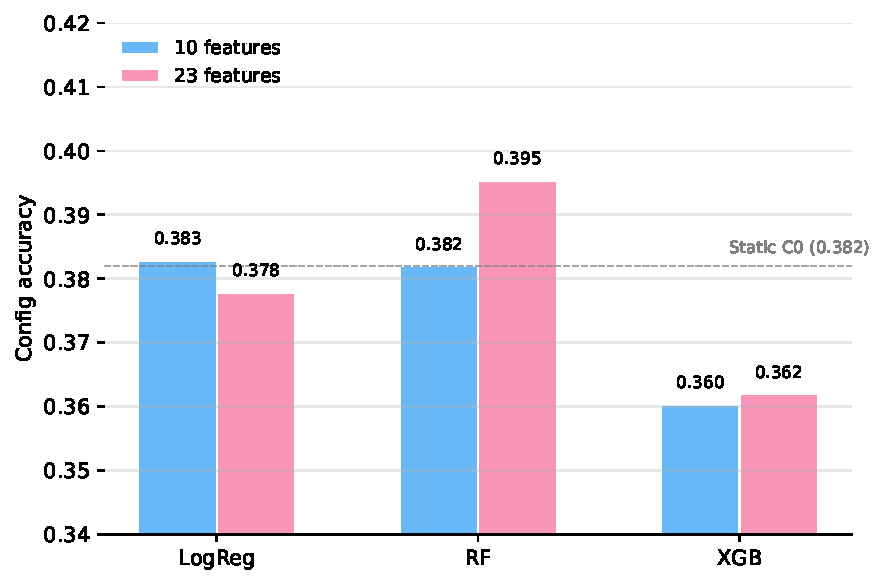
\includegraphics[width=0.55\textwidth]{fig_e1_feature_comparison.pdf}
\caption{Config accuracy: 10 vs 23 features per model.}
\label{fig:e1-comparison}
\end{figure}

This result is expected but requires empirical verification; the response to feature reduction is model-dependent.
LogReg benefits from noise reduction. RF shows the opposite pattern,
despite ``improving'' from 0.382 to 0.395 with the full
set. XGB is indifferent by default.
The low discriminative power of the
10 features confirms that routing signal
is not limited by noise from the remaining features but
by the features' weak prediction capability. Their mean correlation with the oracle label remains below 0.4.


\subsubsection{Metric Sensitivity (E2)}
\label{subsubsec:metric-selection}

The oracle labels depend on which quality metrics define ``pass'' and
at what threshold.  We train a router (RF, 23~features, $\lambda$~sweep)
under each of the seven non-empty subsets of \{fc, faithfulness,
Sup~F1\}, sweeping $\tau \in \{0.5, 0.6, 0.7, 0.8, 0.9\}$.

\begin{figure}[h!]
\centering
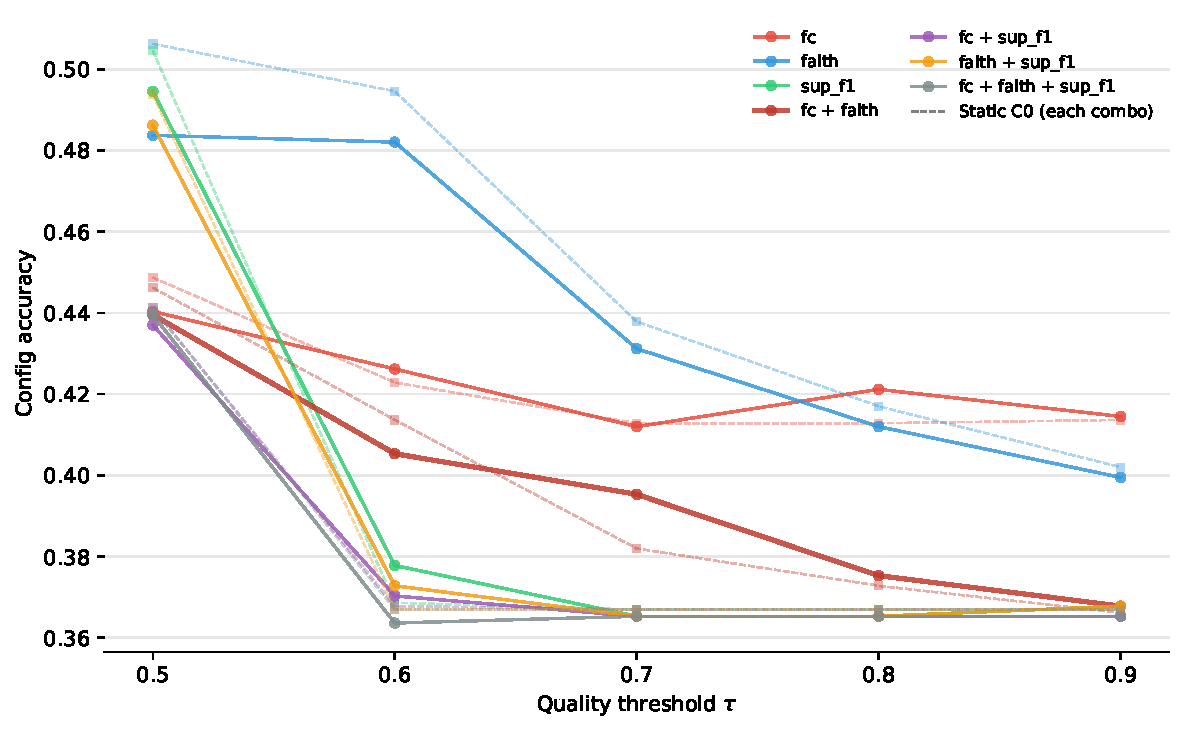
\includegraphics[width=0.85\textwidth]{fig_metric_selection.pdf}
\caption{Config accuracy vs $\tau$ per metric subset}
\label{fig:metric-selection}
\end{figure}

Three regimes emerge in Figure~\ref{fig:metric-selection}:  
\begin{itemize}
      \item At low $\tau$ the oracle is C0-dominated and the router trails its own C0 baseline by 1--2~pp. 
      \item Any combination containing Sup~F1 collapses at $\tau \geq 0.6$ (mean Sup~F1 = 0.545, below threshold).
      \item The fc~+~faith combination occupies a middle regime: at $\tau = 0.7$ the pass rate is 56\% and the
      label distribution is most balanced (C0~38\%, C3~32\%, C2/C6~15\%),
      producing the largest positive margin in the sweep: 0.395 vs
      Static~C0 0.382 (+1.3~pp).  
      \item At stricter thresholds the margin vanishes.
\end{itemize}   

Label learnability depends on the pass-rate regime: too lenient or too
strict both collapse routing to the static baseline.  Noisy quality
metrics (Chapter~\ref{sec:labeling}) further limit the signal any
classifier can exploit (Section~\ref{subsec:ceiling}).


\subsubsection{Cascade Architecture (E3)}
\label{subsubsec:cascade}

All previous strategies commit to the full configuration before
any pipeline component executes.  E3 tests whether deferring the
reranking decision to \emph{midway}---after retrieval---unlocks
additional signal.  Stage~1 predicts search type from query
features (identical to S5); the system executes retrieval; Stage~2
observes five retrieval-quality statistics and decides whether
reranking is needed.  Two variants are tested: V1 uses retrieval
features only (5), V2 adds the 23~query features (28 total).

V1 achieves 0.394 and V2 achieves 0.397---only 0.2~pp above S5.
The Stage~2 reranking classifier reaches AUC~0.53 with retrieval
features alone, barely above random.
Figure~\ref{fig:e7-importance} confirms: three of five retrieval
features rank in the top~10 by RF importance, yet importances are
nearly uniform---a pattern typical of low-signal classification.
The midway signal describes retrieval confidence, not reranking
benefit.

\begin{figure}[h!]
\centering
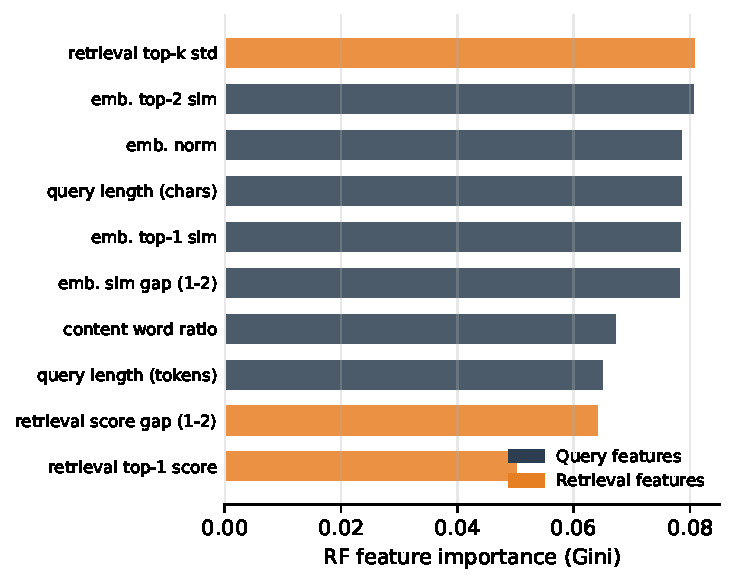
\includegraphics[width=0.6\textwidth]{fig_e7_feature_importance.pdf}
\caption{E3 Stage~2 feature importance}
\label{fig:e7-importance}
\end{figure}


\subsection{The Structural Ceiling}
\label{subsec:ceiling}

The convergence of all approaches to the 0.38--0.40 range is itself a
finding.  Five strategies and three explorations spanning tree-based
classifiers, neural networks and a two-stage cascade all reach the
same region.
The between-experiment spread is 2~pp (0.377--0.397), comparable to the
within-experiment cross-validation standard deviation of 1--2~pp.
Experiment-to-experiment variation is indistinguishable from fold-to-fold
noise.  A McNemar test on the 1{'}200 query-level predictions confirms
this: the difference between S5~RF (0.395) and Static~C0 (0.382) yields
$p = 0.105$ (two-sided exact test, 86~discordant pairs).  The 1.3~pp
margin is not statistically significant at $\alpha = 0.05$ and translates
to 16~additional correctly-routed queries out of 1{'}199.  This indicates a
structural ceiling, not a failure of any individual model.  E2's metric-selection sweep reinforces this: across
35 label definitions (7 metric subsets $\times$ 5 thresholds), only
fc~+~faith at $\tau = 0.7$ produces a positive margin over Static~C0.
All other combinations either collapse to the baseline or track below
it, indicating that the labels themselves carry noise from imperfect
quality metrics.

\paragraph{Lambda as evidence.}
The $\lambda$ analysis in Section~\ref{subsec:strategy-survey} reinforces
this interpretation.  At $\lambda = 0$ (no energy penalty), all models
achieve 0.28--0.35---worse than Static~C0.  Performance rises only as
$\lambda$ increases toward 1.50, which pushes selections toward cheap
configurations unless the classifier is confident.  In practice, this
amounts to a soft version of ``always pick C0'': the utility function,
not the classifier, drives accuracy above baseline.  The ML model's
marginal contribution is the 1--2~pp it adds on top of the $\lambda$-driven
default.

\paragraph{Weak pre-execution signal.}
The strongest feature--label association is Cramér's $V = 0.152$
(\texttt{q\_has\_logical\_operator}, Section~\ref{subsec:features-signal}).
Cross-validated regression on all 23~features yields
$R^2 \approx 0$.  The features capture query-level properties---length,
structure, named entities---but not the query--document interactions that
determine which pipeline modules help.

\paragraph{Small quality differences.}
Factual correctness varies by less than 0.03~points across
\{C0, C2, C3, C6\}.  When the quality surface is nearly flat, any
classifier faces a low signal-to-noise ratio.  The 95\% confidence interval
within a single configuration covers most of the cross-configuration range.

\paragraph{Module-activation vs.\ model routing.}
The quality gap between configurations (2--4~pp) is an order of magnitude
smaller than the gap between models in model routing (10--30~pp),
fundamentally limiting the routing signal.

\paragraph{The information gap.}
The gap between the oracle (100\%) and the best router (39.5\%) quantifies
the information that exists at retrieval time but is invisible before
execution.  E3 confirmed this directly: even after observing
retrieval-quality statistics, the Stage~2 classifier achieves
AUC $\approx 0.53$ for predicting reranking need---barely above random.

Section~\ref{subsec:ceiling-interpretation} discusses the implications of
these observations.


% \subsection{Chapter Summary}
% \label{subsec:ch7-summary}

% Five routing strategies and four controlled experiments were evaluated
% on 1{'}200~HotpotQA queries using 5-fold cross-validation over the
% four no-HyDE configurations.  Three findings emerge:

% \begin{enumerate}
%     \item All approaches converge to a config accuracy of 0.38--0.40,
%           bounded by a structural ceiling.  No combination of features,
%           quality metrics or model architecture breaks through.
%     \item The highest config accuracy observed (0.397, E4 cascade)
%           exceeds Static~C0 by 1.5~pp---a gain within cross-validation
%           noise.  No approach produces a statistically meaningful
%           improvement over the cheapest-configuration baseline.
%     \item The energy penalty parameter $\lambda$ is more impactful than
%           the choice of classifier, feature set or label definition.
%           High $\lambda$ values enforce cheap defaults unless the quality
%           signal is strong, effectively implementing a soft version of
%           Static~C0.
% \end{enumerate}

% The ceiling is signal-limited, not model-limited.  Module-activation
% routing operates on a nearly flat quality surface where pre-execution
% features cannot capture the query--document interactions that determine
% which pipeline modules help.
% Chapter~\ref{sec:discussion} interprets these findings and discusses
% their implications for future research.

\newpage
\section{Discussion}
\label{sec:discussion}

% Chapter purpose: Interpret the structural ceiling alongside quality
% evaluation dependencies and module-space limitations.  Lead with
% information asymmetry, then lambda dominance, then HyDE resolution,
% then quality evaluation, then methodology.  State limitations and
% future directions.


\subsection{Summary of Findings}
\label{subsec:synthesis}

This thesis investigated whether per-query module activation can reduce
energy consumption in locally deployed RAG systems without degrading answer
quality.  Three results, each building on the previous, converge on a
single conclusion.

The baseline analysis (Chapter~\ref{sec:baseline_analysis}) confirmed that
always-on module activation is measurably inefficient.  The full pipeline
costs 5.6$\times$ more energy than the minimal pipeline, while
quality improves by less than 0.06~points on either metric.  The cost is unconditional;
the benefit is conditional and query-dependent.

The decision problem formulation (Chapter~\ref{sec:controller}) quantified
the opportunity.  In the full eight-configuration space, an oracle router
saves 75\% energy versus always-C7(KMS Pipeline) by avoiding HyDE whenever possible.
Restricting to the non-HyDE configurations actually tested for routing
(\{C0, C2, C3, C6\}), the oracle saves 19\% versus always-C6 and 40\%
of queries benefit from routing to a cheaper configuration.  Yet
pre-execution query features explain near-zero variance in quality scores
($R^2 \approx 0$), signalling that even this reduced opportunity may be
difficult to exploit in practice.

The routing investigation (Chapter~\ref{sec:strategies}) confirmed this
difficulty.  Five routing strategies and three explorations, spanning
three model classes, two feature sets and two decision
architectures, all converge to a config accuracy of
0.38--0.40.  No approach produces a statistically meaningful improvement
over the cheapest-configuration baseline (Static~C0 at 0.382).  The
ceiling is signal-limited, not model-limited.


\subsection{Information Asymmetry}
\label{subsec:ceiling-interpretation}

The convergence of all routing strategies to the same narrow performance
band is the thesis's central empirical finding.  The 60.5~percentage-point
gap between oracle (100\%) and best router (39.5\%) is not a failure of
modeling.  It quantifies information that exists at retrieval time but is
invisible before pipeline execution.  This section interprets the nature
of this asymmetry and what it implies for the field.

\paragraph{A circular dependency.}
Accurate routing requires post-retrieval signals: document scores,
score gaps, source diversity.  The purpose of routing is to avoid
executing retrieval variants that would produce those signals.  This
creates a circular dependency: the information needed to route is
produced by the very computation that routing aims to skip.

Experiment E3 (Section~\ref{subsec:explorations})
tested this directly.  Even after observing C0 retrieval statistics,
the Stage~2 reranking classifier achieved AUC~$\approx 0.53$, barely
above random.  The retrieval statistics answer ``how good was this
retrieval?'' but not ``would a different retrieval strategy help this
query?''  These are structurally different questions.

\paragraph{Module-activation vs.\ model routing.}
Table~\ref{tab:routing-comparison} contrasts three routing granularities.
Model routing selects \emph{who answers}: the query goes to a strong or
weak LLM with the same context.  Module-activation routing selects
\emph{how to prepare the context}: which retrieval and post-retrieval
stages run before generation.  The quality gap that a router must
discriminate shrinks by an order of magnitude from model selection
(10--30~pp) to module activation (2--4~pp), which directly limits the
signal available to any classifier.

\begin{table}[h!]
\centering
\small
\begin{tabular}{l l c l}
\hline
\textbf{System} & \textbf{Granularity} & \textbf{Quality gap} & \textbf{Reported savings} \\
\hline
RouteLLM~\cite{routellm2025}   & Model selection   & 10--30~pp & 50--85\% cost reduction \\
FrugalGPT~\cite{frugalgpt2023} & Model cascade     & 10--30~pp & up to 98\% cost reduction \\
This work                       & Module activation & 2--4~pp   & 39.5\% config accuracy \\
\hline
\end{tabular}
\caption{Routing approaches by granularity.}
\label{tab:routing-comparison}
\end{table}

In model routing, a router discriminates between generators that produce
10--30~pp quality gaps on identical context.  In our module routing setup,
the same generator receives slightly different retrieval preparations,
compressing the quality gap to 2--4~pp while within-config noise stays
constant.  Systems with larger module-level quality variation may face a
more tractable routing problem.  Adaptive RAG systems
(Self-RAG~\cite{selfrag2024}, CRAG~\cite{crag2024},
Adaptive-RAG~\cite{adaptiverag2024}) operate at the strategy level where
quality differences remain large enough to learn.  In our test case,
finer-grained module control faces a structurally harder prediction
problem.

\paragraph{Signal-limited, not model-limited.}
Because the ceiling is signal-limited, investing in more sophisticated
classifiers (deeper networks, larger training sets, richer architectures)
is unlikely to yield improvements within the current feature
space.  The between-experiment accuracy spread (2~pp) is comparable to
within-experiment cross-validation noise (1--2~pp).  The rational response
is to deploy the simplest approach that captures the available signal and
invest research effort in cheaper ways to access post-retrieval
information.

\paragraph{Characterising the boundary.}
Defining a ceiling has methodological value.  The experiments
consistently place the boundary at 0.38--0.40 config accuracy for
pre-execution features on module-activation routing, empirically
validated across five strategies and three explorations.  This delimits
where future work is unlikely to yield gains under similar assumptions
and identifies what is needed to break through: cheaper access to
post-retrieval signals.  The 60.5~pp gap between oracle and achieved
performance defines a concrete, quantified research target.


\subsection{Energy Penalty ($\lambda$) Analysis}
\label{subsec:lambda}

Perhaps the most actionable finding is that the energy penalty
parameter~$\lambda$ matters more than the choice of classifier, feature
set or model architecture.  Across all experiments, the best results
appear at $\lambda = 1.25$--$1.50$.  Without the energy penalty
($\lambda = 0$), all models achieve 0.28--0.35, worse than Static~C0.
Performance rises only as $\lambda$ increases, which pushes selections
toward cheap configurations unless the classifier is confident.  In
practice, this amounts to a soft version of ``always pick C0'': the
utility function, not the classifier, drives accuracy above baseline.

This observation shifts the RAG efficiency problem from a machine learning
problem to a policy problem.  A high~$\lambda$ implements a
cheap-by-default policy: expensive modules are assumed unnecessary unless
the quality signal strongly indicates otherwise.  For locally deployed
systems with constrained energy budgets, this policy is the most
defensible strategy.  It requires no additional model, no training
infrastructure and no runtime overhead beyond the utility calculation.

The classifier's marginal contribution is the 1--2~pp it adds on top of
the $\lambda$-driven default.  Tuning a single scalar parameter
outperforms all model-selection experiments in this thesis.


\subsection{The HyDE Variance}
\label{subsec:hyde}

Hypothetical Document Embeddings (HyDE)~\cite{hyde2023} is widely
reported as beneficial in RAG pipelines, particularly for bridging
vocabulary gaps between queries and documents.  Our results contradict
this: HyDE degrades quality ($-$0.013~fc, $-$0.021~faithfulness) at
5.3$\times$ the energy cost of the minimal pipeline.  This led to its
exclusion from the routing configuration space.

The contradiction likely reflects an interaction between HyDE and the
retrieval architecture.  HyDE was designed for sparse retrieval systems
where lexical mismatch dominates.  In our dense-retrieval setup using
BGE-M3, the embedding model already bridges vocabulary gaps.  We
hypothesise that the hypothetical document generated by the LLM pushes
the query embedding into semantically adjacent but factually irrelevant
regions of the vector space.  Where sparse retrieval benefits from
vocabulary expansion, dense retrieval suffers from what we term
\emph{semantic drift}: the hypothetical introduces noise into an already
well-positioned query vector.  Confirming this hypothesis requires
comparing query and hypothetical-document embeddings directly in the
vector space and remains an open direction for future work.

This result does not invalidate HyDE as a technique.  It demonstrates
that module utility is system-dependent: a component that improves one
retrieval architecture may degrade another.  The 75\% oracle energy
saving in the full configuration space is primarily an engineering
decision (disabling a harmful module), while the 19\% saving in the
non-HyDE routing space is the algorithmic ceiling for per-query routing.
These two numbers quantify different opportunities: the first is
immediately actionable, the second defines the research target.


\subsection{Methodological Legacy}
\label{subsec:methodology}

The measurement framework developed in
Chapter~\ref{sec:method_protocol} is the most transferable artifact of
this thesis.  The framework implements three design principles:
session-scoped energy counters, pipeline-stage markers and per-node
attribution.  These generalise to any distributed system with toggleable
components.  The instrumentation code, configuration API and analysis
pipeline are available as part of the CITI~KMS repository.  While the
absolute energy numbers are system-specific, the methodology enables any
modular RAG deployment to quantify its own trade-offs and assess routing
potential without modifying pipeline stages.

\paragraph{Quality evaluation.}
The routing pipeline depends on quality labels, which depend on evaluation
metrics, which depend on the evaluator model.  This dependency chain
(evaluator $\to$ thresholds $\to$ labels $\to$ routing signal) means
that evaluation quality propagates through every downstream result.
If the labels are unreliable, no classifier can learn a meaningful
decision boundary regardless of feature strength.

We use Qwen2.5-14B-Instruct as evaluator and a different model family
(R-4B) as generator, avoiding self-evaluation bias where models favour
their own generation patterns~\cite{vrageval2024}.  Wang~et~al.\ report
that evaluator size determines reliability: 8B~models achieve 36.8\%
human agreement on binary accept/reject versus 82.6\% for
GPT-4-class models.  Our 14B~evaluator sits between these extremes.
The choice of RAGAS was driven by its existing integration within the
system infrastructure; methodologically, it operationalises the
LLM-as-a-judge paradigm by decomposing answers into verifiable
claims~\cite{ragevalsurvey2025}.  Any inconsistency in the judge's
scoring propagates directly into the routing labels.  A comparison with
alternative frameworks (ARES, vRAG-Eval) would verify whether the
structural ceiling is judge-invariant.

The ICC analysis in Section~\ref{subsec:quality-labeling} shows that each
metric privileges a different aspect of the pipeline.  Answer~F1
(ICC\,=\,0.825) captures lexical overlap but treats all configurations as
near-interchangeable, making it unsuitable for routing supervision.
Faithfulness (ICC\,=\,0.432) has the strongest between-configuration
variance but evaluates generation consistency rather than factual
accuracy.  Factual correctness (ICC\,=\,0.583) balances the two but
depends on the evaluator model's decomposition of claims.  The E2
exploration (Section~\ref{subsec:explorations}) confirms that the metric
choice is decisive: only factual correctness combined with faithfulness
at $\tau = 0.7$ produces a positive routing margin; all other combinations
collapse to baseline or below.

For a knowledge management deployment, the priority is whether the answer
contains the correct information (factual correctness) and does not
fabricate unsupported claims (faithfulness).  Lexical overlap with a
reference answer matters less when users seek explanations rather than
exact phrases.  The structural ceiling of 0.38--0.40 config accuracy may
therefore reflect not only information asymmetry but also label noise from
imperfect evaluation.  These two sources of difficulty compound: even if
corpus-aware features provided stronger signal, noisy labels would limit
what a classifier can learn from them.  Establishing a validated,
domain-appropriate quality evaluation method is the logical first step
before investing in richer routing features.


\subsection{Limitations}
\label{subsec:limitations}

Several limitations constrain the generalisability of these findings.

\paragraph{System generalisability.}
All experiments use the CITI~KMS pipeline with a specific LLM size,
embedding model, retrieval backend and three toggleable modules (HyDE,
reranking, hybrid search) inherited from the existing system rather than
selected from a systematic survey.  Advanced RAG architectures offer
additional modules---query decomposition, web-search fallback
(CRAG~\cite{crag2024}), self-reflective generation
(Self-RAG~\cite{selfrag2024}), document summarisation, answer
verification---each with different energy costs.  The 2--4~pp quality gap
may be specific to this module set; a broader module space could produce
a more tractable routing problem.  All measurements also assume
single-request sequential execution; concurrent workloads may change
energy patterns due to resource contention and GPU utilisation differences.
The absolute numbers (e.g., 5.6$\times$ energy ratio) are
system-specific; the methodology and ceiling characterisation approach
generalise.

\paragraph{Dataset scope and feature transferability.}
HotpotQA provides multi-hop reasoning queries only, and the experiment
uses a corpus built from gold supporting documents.  In open-domain
retrieval, where relevant documents may be absent or diluted, the quality
surface may differ and could create stronger routing signals.  The two
most important routing predictors are dataset-specific:
\texttt{q\_has\_logical\_operator} appears in 61\% of HotpotQA queries
versus 22\% of KILT queries (39~pp gap), and \texttt{q\_multi\_entity}
in 76\% versus 45\% (31~pp gap).  Both features reflect multi-hop
structure rather than a general query property.  A router trained on
these features would encounter a substantially different input
distribution on factoid or verification queries, limiting
transferability without retraining.

\paragraph{Title-level provenance evaluation.}
HotpotQA annotates supporting facts as (title, sentence\_id) pairs; the
official Sup~F1 operates at sentence granularity.  Our system chunks
Wikipedia articles by character count (1{'}024-character windows with
200-character overlap), not by sentence boundaries.  Our Sup~F1 evaluates
at title level and is not directly comparable to leaderboard scores.

\paragraph{LLM-as-judge evaluation.}
Quality evaluation relies on RAGAS with Qwen2.5-14B-Instruct as the
evaluator model.  LLM-based evaluation introduces its own biases.  We
mitigate this by using the same evaluator consistently across all
configurations, so relative comparisons remain valid even if absolute
scores carry systematic bias.

\paragraph{Limited feature set.}
The 23~pre-execution features are a first attempt at characterising query
difficulty for routing.  Richer features (query--document interaction
signals, LLM self-assessment or lightweight retrieval probes) may carry
stronger discriminative power, though the ceiling analysis suggests this
is unlikely without accessing post-retrieval information.


\subsection{Future Directions}
\label{subsec:future}

The ceiling finding defines the research agenda: how to access
post-retrieval information without incurring its full cost.

\paragraph{Lightweight retrieval probing.}
The circular dependency can be partially broken if a cheap retrieval
approximation provides routing-relevant signal.  A sparse retrieval
probe (e.g., BM25) that costs milliseconds rather than seconds could
estimate whether hybrid search or reranking would help a specific query.
If a BM25 score gap predicts reranking benefit, the router gains access
to post-retrieval signals at a fraction of the pipeline cost.

\paragraph{Transfer to model routing.}
Module-activation routing faces quality gaps of 2--4~percentage points;
model routing faces gaps of 10--30~pp.  Investigating whether the same
query features that fail for module routing succeed for model routing
would clarify the relationship between signal strength and routing
granularity.  Success would confirm that the ceiling is specific to
fine-grained module control, not to query-feature-based routing in
general.

\paragraph{Multi-task workloads.} A production RAG system serves diverse query types.  Different query
types (factoid, verification, multi-hop) may create more separable
routing populations.  Routing accuracy may improve when the training
set spans multiple task distributions with larger between-type
quality variation.

\paragraph{Non-routable query detection.} The 445~queries (37\%) that fail under all eight configurations represent
a system quality limitation, not a routing limitation.  If non-routable
queries are detectable pre-execution, a router could abstain rather than
waste energy on queries likely to fail regardless.  This binary
distinction may be more tractable than configuration selection, since the
routable/non-routable gap is larger than the 2--4~pp quality gap between
configurations.

\paragraph{Online learning.} Adapting the routing policy from production feedback using contextual
bandits or reinforcement learning would enable continuous improvement
without requiring forced-run experiments.  This is particularly relevant
because the quality landscape may shift as the document corpus evolves.

\paragraph{Corpus-aware embedding features.}
The 23~pre-execution features characterise queries in isolation from the
indexed document collection.  Since BGE-M3 embeddings already exist for
all indexed documents, principal component analysis of the corpus
embedding space could yield routing features at negligible cost.
Projecting each query into the first 100--150 principal components of the
document cloud enables features such as distance to the corpus centroid,
local document density and cluster membership.  UniRoute~\cite{uniroute2025}
provides theoretical grounding for cluster-based routing, demonstrating
Bayes-optimal routing with bounded excess risk when queries are assigned
to corpus clusters.  These features partially break the circular
dependency (Section~\ref{subsec:ceiling-interpretation}) by providing
corpus awareness without executing retrieval variants.  They remain
pre-execution, so they cannot access actual retrieved document quality,
but they represent a middle ground between query-only surface features
and the full cost of post-retrieval signals.

\paragraph{Broader module evaluation.}
The three modules tested in this work span query expansion, retrieval
strategy and post-retrieval filtering.  Production RAG systems may
include additional stages: query decomposition for complex questions,
web-search fallback for corpus gaps, answer verification against retrieved
evidence or document summarisation before generation.  Each module
introduces a different energy--quality trade-off.  Systematically
evaluating the quality contribution of each candidate module---before
attempting to route among them---would establish which modules produce
quality differences large enough to be learnable by a pre-execution
router.

\paragraph{Energy measurement under concurrent workloads.}
Extending the measurement framework to multi-tenant scenarios would
quantify how resource contention affects per-request energy attribution
and whether routing decisions remain valid under production load.

\newpage
\section{Conclusion}
\label{sec:conclusion}


This thesis investigated energy-aware configuration control for locally
deployed RAG systems, asking whether per-query module activation can
reduce energy consumption without degrading answer quality.  We
hypothesised that a circular dependency limits pre-execution routing:
the information needed to select modules is produced by executing those
modules.

We designed a measurement framework that attributes energy, latency and
quality to individual pipeline modules across infrastructure nodes.
Applying it to the CITI KMS system with 1{'}200~HotpotQA queries across
eight configurations (9{'}600 sessions), we established three findings.

First, always-on module activation is measurably inefficient.  The full
pipeline consumes 5.6$\times$ more energy than the minimal pipeline, while
quality improves by less than 0.06~points on either metric.  The cost is
unconditional; the benefit is conditional and query-dependent.

Second, an oracle router saves 75\% energy versus always-C7, but this
is primarily an engineering decision: disabling HyDE, which degrades
quality at 5.3$\times$ the energy cost.  In the non-HyDE space
(\{C0, C2, C3, C6\}), the oracle ceiling drops to 19\% versus
always-C6.  The 75\% quantifies removing a harmful module; the 19\%
quantifies the algorithmic routing limit.

Third, eight routing experiments (five strategies, three explorations)
all converge to a config accuracy of 0.38--0.40, with no statistically
meaningful improvement over the cheapest-configuration baseline.  The
ceiling is signal-limited: pre-execution features cannot capture the
query--document interactions that determine which modules help.  The
information needed to route is produced by the computation routing aims
to skip.

These results yield four contributions:

\begin{enumerate}
    \item \textbf{Contribution 1}: An energy measurement framework for distributed RAG
          systems that attributes cost per module, per node and per
          stage, reusable for any modular RAG pipeline.
    \item \textbf{Contribution 2}: Empirical evidence that always-on module activation
          is inefficient, with energy costs spanning 5.6$\times$ for
          quality differences below 0.06~points on either metric.
    \item \textbf{Contribution 3}: A systematic routing investigation that quantifies
          the signal boundary for pre-execution module prediction.
          Module-activation routing is harder than model routing because
          quality gaps between configurations (2--4~pp) are an order of
          magnitude smaller than between models (10--30~pp).
    \item \textbf{Contribution 4}: Characterisation of the information gap between
          oracle routing (100\% config accuracy) and achievable
          pre-execution routing (39.5\%), defining a concrete research
          target: cheaper access to post-retrieval signals.
\end{enumerate}

The 60.5~percentage-point gap between oracle and achieved performance
is the thesis's most consequential result: a structural property of
module-activation routing with pre-execution features, not a limitation
to overcome within the current paradigm.  Closing this gap requires
post-retrieval information at a cost lower than the computation it
replaces.  Meanwhile, a well-tuned energy penalty~$\lambda$ captures
most achievable benefit without any learned model, reducing the problem
to a policy decision rather than a machine learning task.


% Appendix
% !TEX root = ../main.tex
\newpage
\appendix


% ============================================================================
% A P P E N D I X   A :   R O U T I N G   R E S U L T S
% ============================================================================

\section{Consolidated Routing Results}
\label{app:routing-results}

Table~\ref{tab:app-routing} reports the best policy per experiment across
all routing investigations.  Seven experiments (E1--E7) extend the five
strategies described in Section~\ref{sec:strategies} by varying the feature
set, quality metric definition and decision architecture.  All experiments
use 5-fold stratified cross-validation on $N = 1{'}200$ queries with the
non-HyDE configuration space \{C0, C2, C3, C6\}.

\begin{table}[H]
\centering
\small
\begin{tabular}{l l l r r r r}
\hline
\textbf{Experiment} & \textbf{Best model} & $\bm{\lambda}$ & \textbf{Acc} & \textbf{F1\textsubscript{m}} & \textbf{Pass} & \textbf{E (J)} \\
\hline
Oracle          & ---         & ---  & 1.000 & 1.000 & 0.555 & 341 \\
\hline
E1: Feature sel.       & LogReg & 1.25 & 0.383 & 0.163 & 0.324 & 318 \\
E2: Full features      & RF     & 1.50 & 0.395 & 0.189 & 0.328 & 318 \\
E3: Retrieval probe    & RF     & 1.50 & 0.384 & 0.176 & 0.319 & 318 \\
E4: Rich features      & RF     & 1.00 & 0.380 & 0.198 & 0.327 & 317 \\
E5: Neural (energy)    & NN     & 1.50 & 0.377 & 0.150 & 0.316 & 319 \\
E6: Neural (rich)      & NN     & 1.50 & 0.383 & 0.165 & 0.318 & 317 \\
E7: Cascade            & RF+RF  & 1.50 & 0.397 & 0.192 & 0.331 & 318 \\
\hline
Static C0       & ---         & ---  & 0.382 & 0.138 & 0.318 & 318 \\
Static C3       & ---         & ---  & 0.318 & 0.121 & 0.323 & 324 \\
Random          & ---         & ---  & 0.256 & 0.245 & 0.335 & 372 \\
\hline
\end{tabular}
\caption{Best policy per routing experiment.
         Acc = config accuracy, F1\textsubscript{m} = F1 macro,
         Pass = pass rate, E = mean energy per request.}
\label{tab:app-routing}
\end{table}

Table~\ref{tab:app-routing-models} breaks down each experiment by
classifier to show that the accuracy plateau holds regardless of model
choice.  The spread within each experiment (1--2~pp) is comparable to
cross-validation noise.

\begin{table}[H]
\centering
\small
\begin{tabular}{l l l r r r}
\hline
\textbf{Experiment} & \textbf{Model} & $\bm{\lambda}$ & \textbf{Acc} & \textbf{F1\textsubscript{m}} & \textbf{Pass} \\
\hline
\multirow{3}{*}{E1: Feature sel.}
  & LogReg & 1.25 & 0.383 & 0.163 & 0.324 \\
  & RF     & 1.50 & 0.382 & 0.187 & 0.327 \\
  & XGB    & 1.50 & 0.360 & 0.203 & 0.326 \\
\hline
\multirow{3}{*}{E2: Full features}
  & LogReg & 1.25 & 0.378 & 0.189 & 0.322 \\
  & RF     & 1.50 & 0.395 & 0.189 & 0.328 \\
  & XGB    & 1.50 & 0.362 & 0.206 & 0.332 \\
\hline
\multirow{3}{*}{E3: Retrieval probe}
  & LogReg & 1.25 & 0.370 & 0.185 & 0.321 \\
  & RF     & 1.50 & 0.384 & 0.176 & 0.319 \\
  & XGB    & 0.50 & 0.369 & 0.228 & 0.324 \\
\hline
\multirow{3}{*}{E7: Cascade}
  & LR+LR  & 1.50 & 0.376 & 0.173 & 0.320 \\
  & RF+RF  & 1.50 & 0.397 & 0.192 & 0.331 \\
  & XGB+XGB & 1.50 & 0.356 & 0.202 & 0.325 \\
\hline
\end{tabular}
\caption{Per-model results within each experiment (best $\lambda$ per model).}
\label{tab:app-routing-models}
\end{table}


% ============================================================================
% A P P E N D I X   B :   A D D I T I O N A L   F I G U R E S
% ============================================================================

\section{Additional Routing Figures}
\label{app:routing-figures}

Figures~\ref{fig:app-pareto}--\ref{fig:app-cm-s6} supplement
the routing analysis of Chapter~\ref{sec:strategies}.

\begin{figure}[H]
\centering
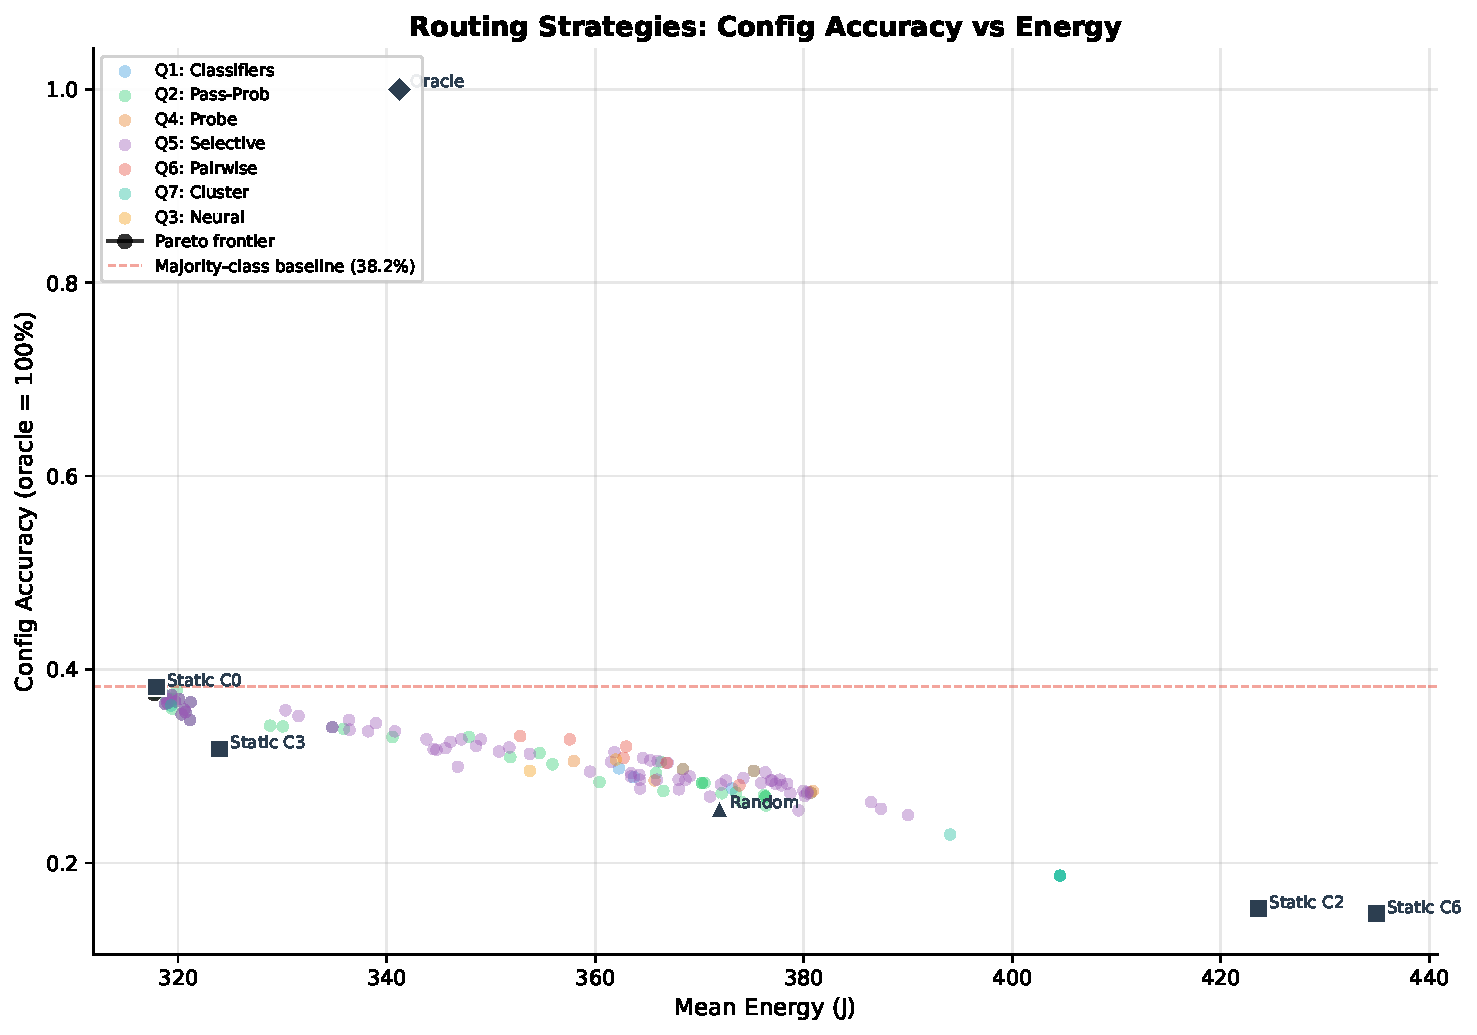
\includegraphics[width=0.85\textwidth]{fig_pareto_frontier.pdf}
\caption{Pareto frontier: config accuracy versus mean energy}
\label{fig:app-pareto}
\end{figure}

\begin{figure}[H]
\centering
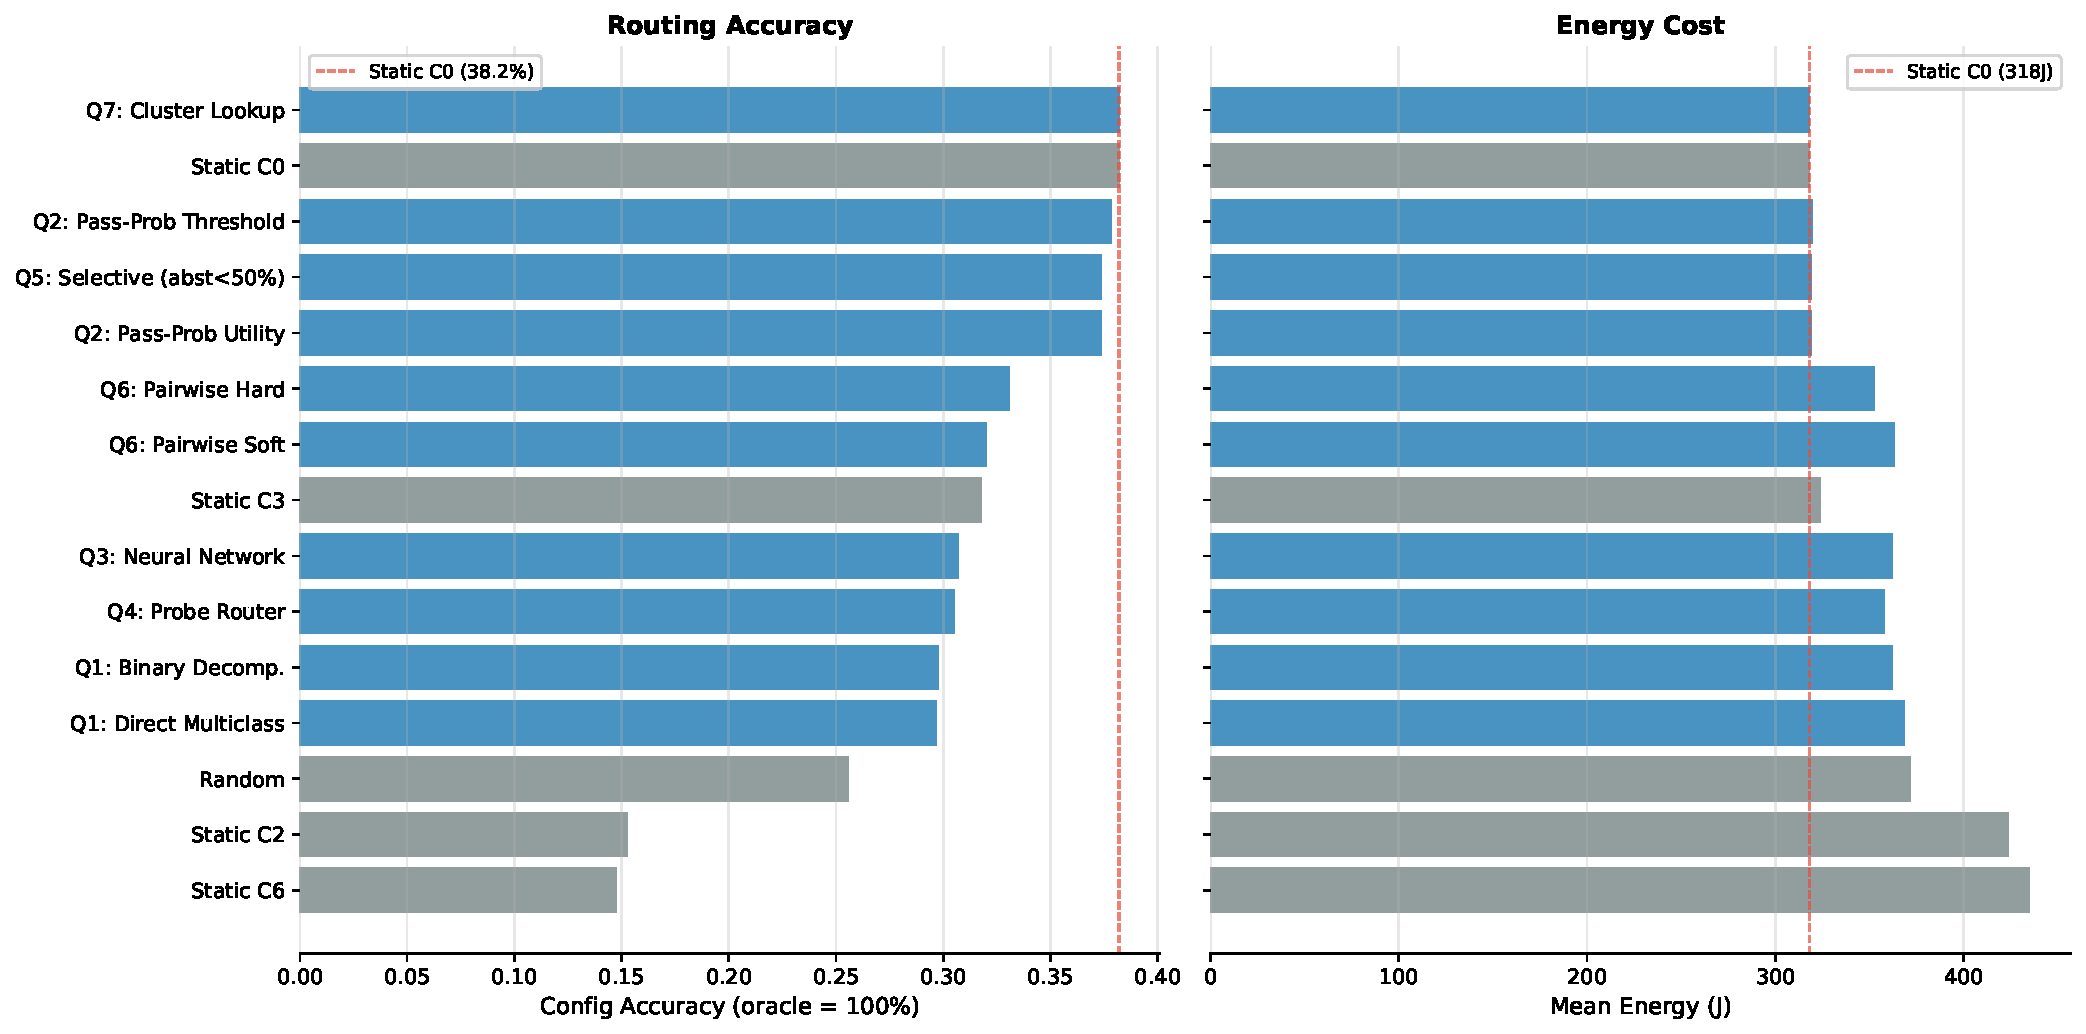
\includegraphics[width=0.95\textwidth]{fig_config_acc_energy_bars.pdf}
\caption{Config accuracy and energy cost per strategy}
\label{fig:app-acc-energy-bars}
\end{figure}

\begin{figure}[H]
\centering
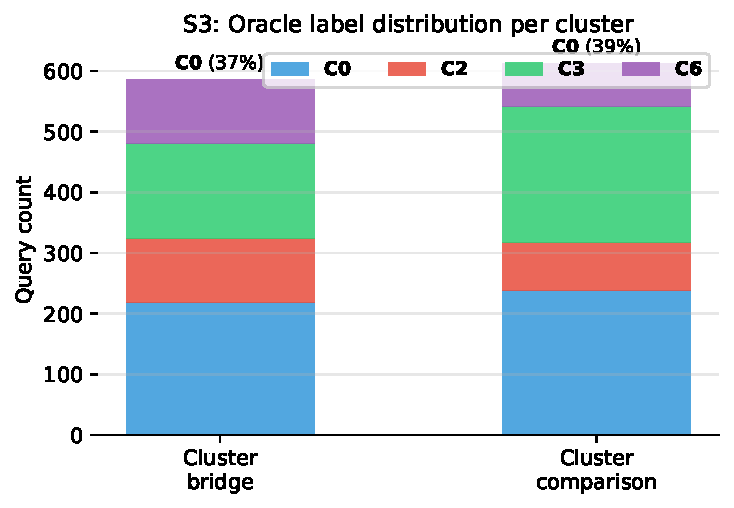
\includegraphics[width=0.65\textwidth]{fig_s3_cluster_lookup.pdf}
\caption{Cluster-based configuration lookup (S3)}
\label{fig:app-s3-cluster}
\end{figure}

\begin{figure}[H]
\centering
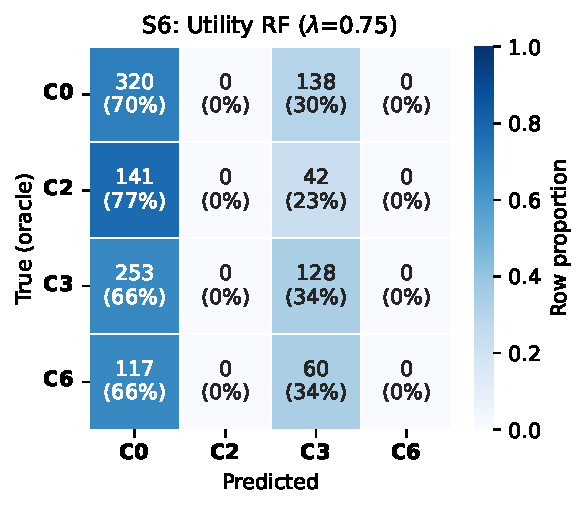
\includegraphics[width=0.55\textwidth]{fig_cm_s6_utility.pdf}
\caption{Confusion matrix for utility scoring variant S6}
\label{fig:app-cm-s6}
\end{figure}


% ============================================================================
% A P P E N D I X   C :   F E A T U R E   S T A T I S T I C S
% ============================================================================

\section{Feature Association Statistics}
\label{app:feature-stats}

Tables~\ref{tab:app-chi2} and~\ref{tab:app-kw} report the full
statistical test results for feature--label association, supporting
the analysis in Section~\ref{subsec:features-signal}.

\paragraph{Boolean features.}
Table~\ref{tab:app-chi2} reports chi-squared tests for all seven boolean
features against the oracle label.
Only \texttt{q\_has\_logical\_operator}
reaches conventional significance ($p < 0.001$), consistent with the
weak-signal finding in the main text.

\begin{table}[H]
\centering
\small
\begin{tabular}{l r r r}
\hline
\textbf{Feature} & $\bm{\chi^2}$ & \textbf{$p$-value} & \textbf{Cram\'er's $V$} \\
\hline
\texttt{q\_has\_logical\_operator} & 27.52 & $<$0.001 & 0.152 \\
\texttt{q\_has\_date\_entity}      & 15.55 & 0.030    & 0.114 \\
\texttt{q\_is\_definition}         & 10.93 & 0.142    & 0.095 \\
\texttt{q\_multi\_entity}          &  8.96 & 0.255    & 0.086 \\
\texttt{q\_has\_number\_entity}    &  4.88 & 0.674    & 0.064 \\
\texttt{reasoning\_marker}         &  4.25 & 0.751    & 0.060 \\
\texttt{has\_code}                 &  3.27 & 0.859    & 0.052 \\
\hline
\end{tabular}
\caption{Chi-squared tests for boolean features versus oracle label ($df = 7$).}
\label{tab:app-chi2}
\end{table}

\paragraph{Numeric features.}
Table~\ref{tab:app-kw} reports Kruskal-Wallis tests for all twelve
numeric features.  Effect sizes ($\eta^2$) remain below 0.02 throughout,
confirming that no single numeric feature explains meaningful label variance.

\begin{table}[H]
\centering
\small
\begin{tabular}{l r r r}
\hline
\textbf{Feature} & \textbf{$H$} & \textbf{$p$-value} & $\bm{\eta^2}$ \\
\hline
\texttt{q\_len\_tokens}             & 22.48 & 0.002   & 0.013 \\
\texttt{q\_len\_chars}              & 18.78 & 0.009   & 0.010 \\
\texttt{q\_ner\_type\_diversity}    & 17.44 & 0.015   & 0.009 \\
\texttt{q\_ner\_count}              & 16.38 & 0.022   & 0.008 \\
\texttt{q\_emb\_sim\_gap}           & 10.40 & 0.167   & 0.003 \\
\texttt{q\_np\_count}               &  8.38 & 0.300   & 0.001 \\
\texttt{num\_sentences}             &  7.40 & 0.389   & $<$0.001 \\
\texttt{q\_emb\_norm}               &  7.00 & 0.429   & $<$0.001 \\
\texttt{q\_content\_word\_ratio}    &  6.42 & 0.492   & $<$0.001 \\
\texttt{q\_emb\_top1\_sim}          &  5.59 & 0.588   & $<$0.001 \\
\texttt{q\_emb\_top2\_sim}          &  4.58 & 0.710   & $<$0.001 \\
\texttt{constraint\_count}          &  3.31 & 0.855   & $<$0.001 \\
\hline
\end{tabular}
\caption{Kruskal-Wallis tests for numeric features versus oracle label ($k = 8$ groups).}
\label{tab:app-kw}
\end{table}


% ============================================================================
% A P P E N D I X   D :   E N E R G Y   D E T A I L S
% ============================================================================

\section{Energy Measurement Details}
\label{app:energy-details}

Figures~\ref{fig:app-cpu-gpu}--\ref{fig:app-power} supplement the
baseline analysis of Chapter~\ref{sec:baseline_analysis} with
node-level and stage-level decompositions.

\begin{figure}[H]
\centering
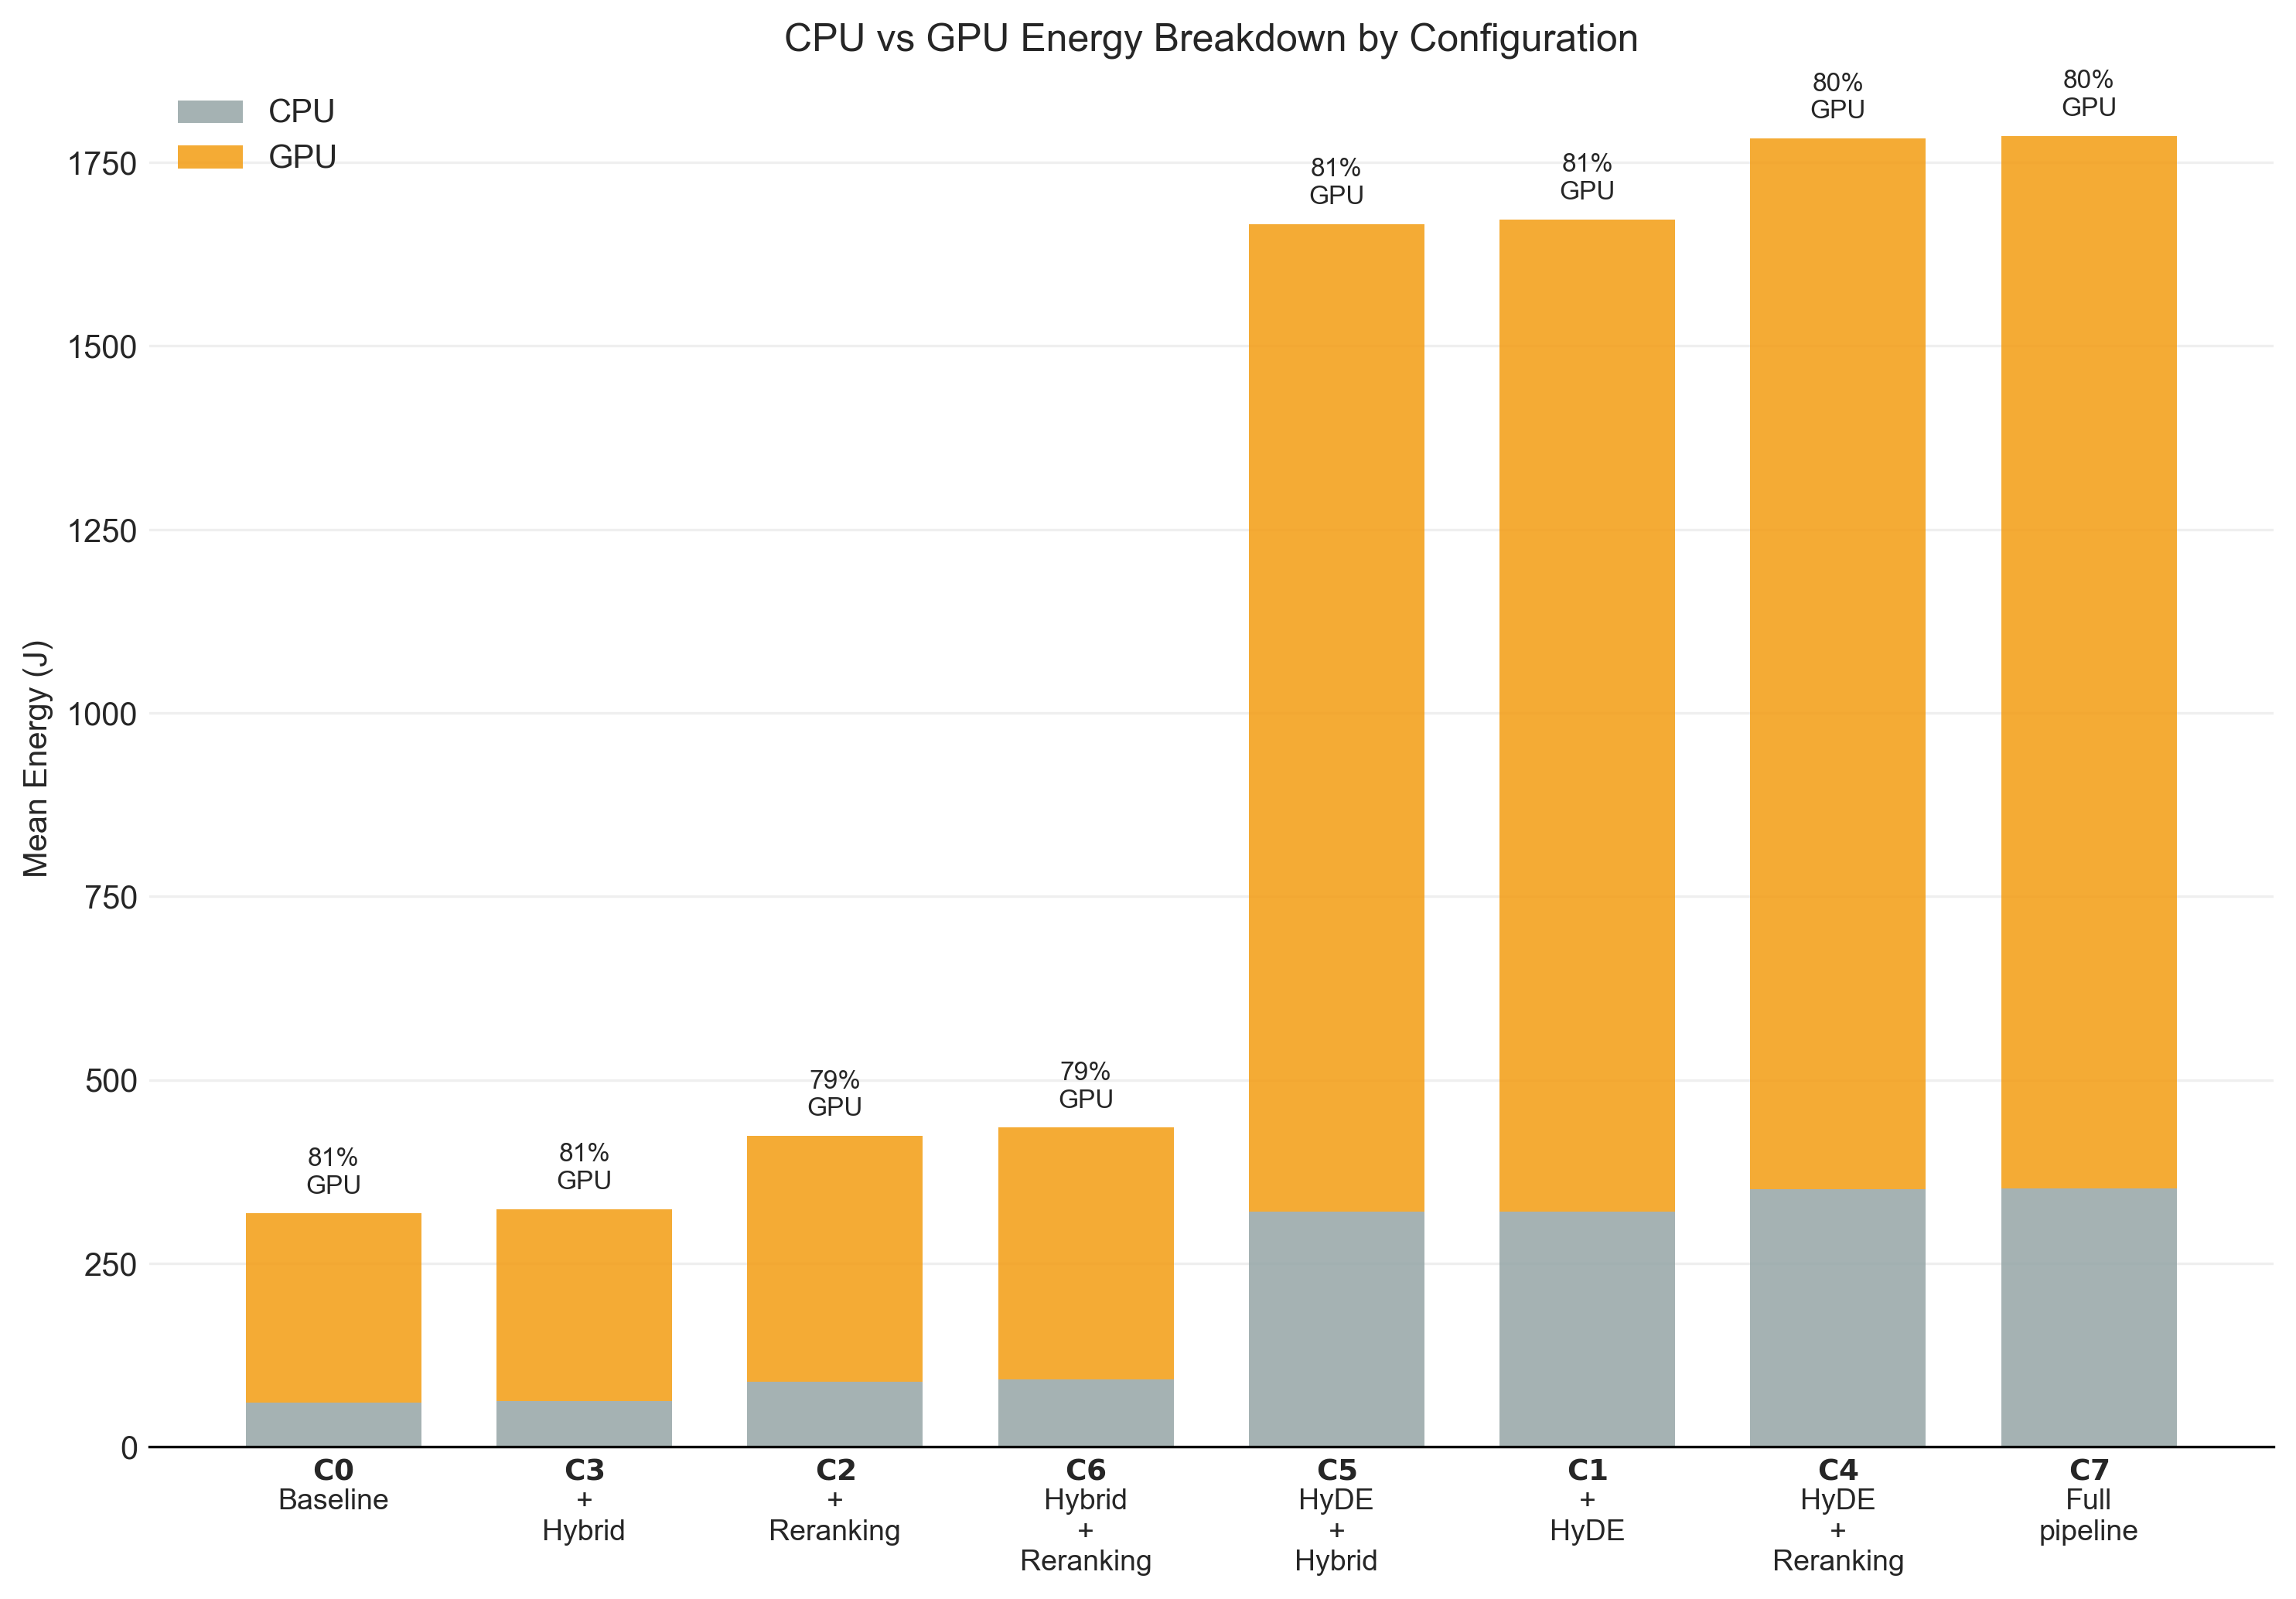
\includegraphics[width=0.85\textwidth]{cpu_gpu_breakdown.png}
\caption{CPU versus GPU energy share per node}
\label{fig:app-cpu-gpu}
\end{figure}

\begin{figure}[H]
\centering
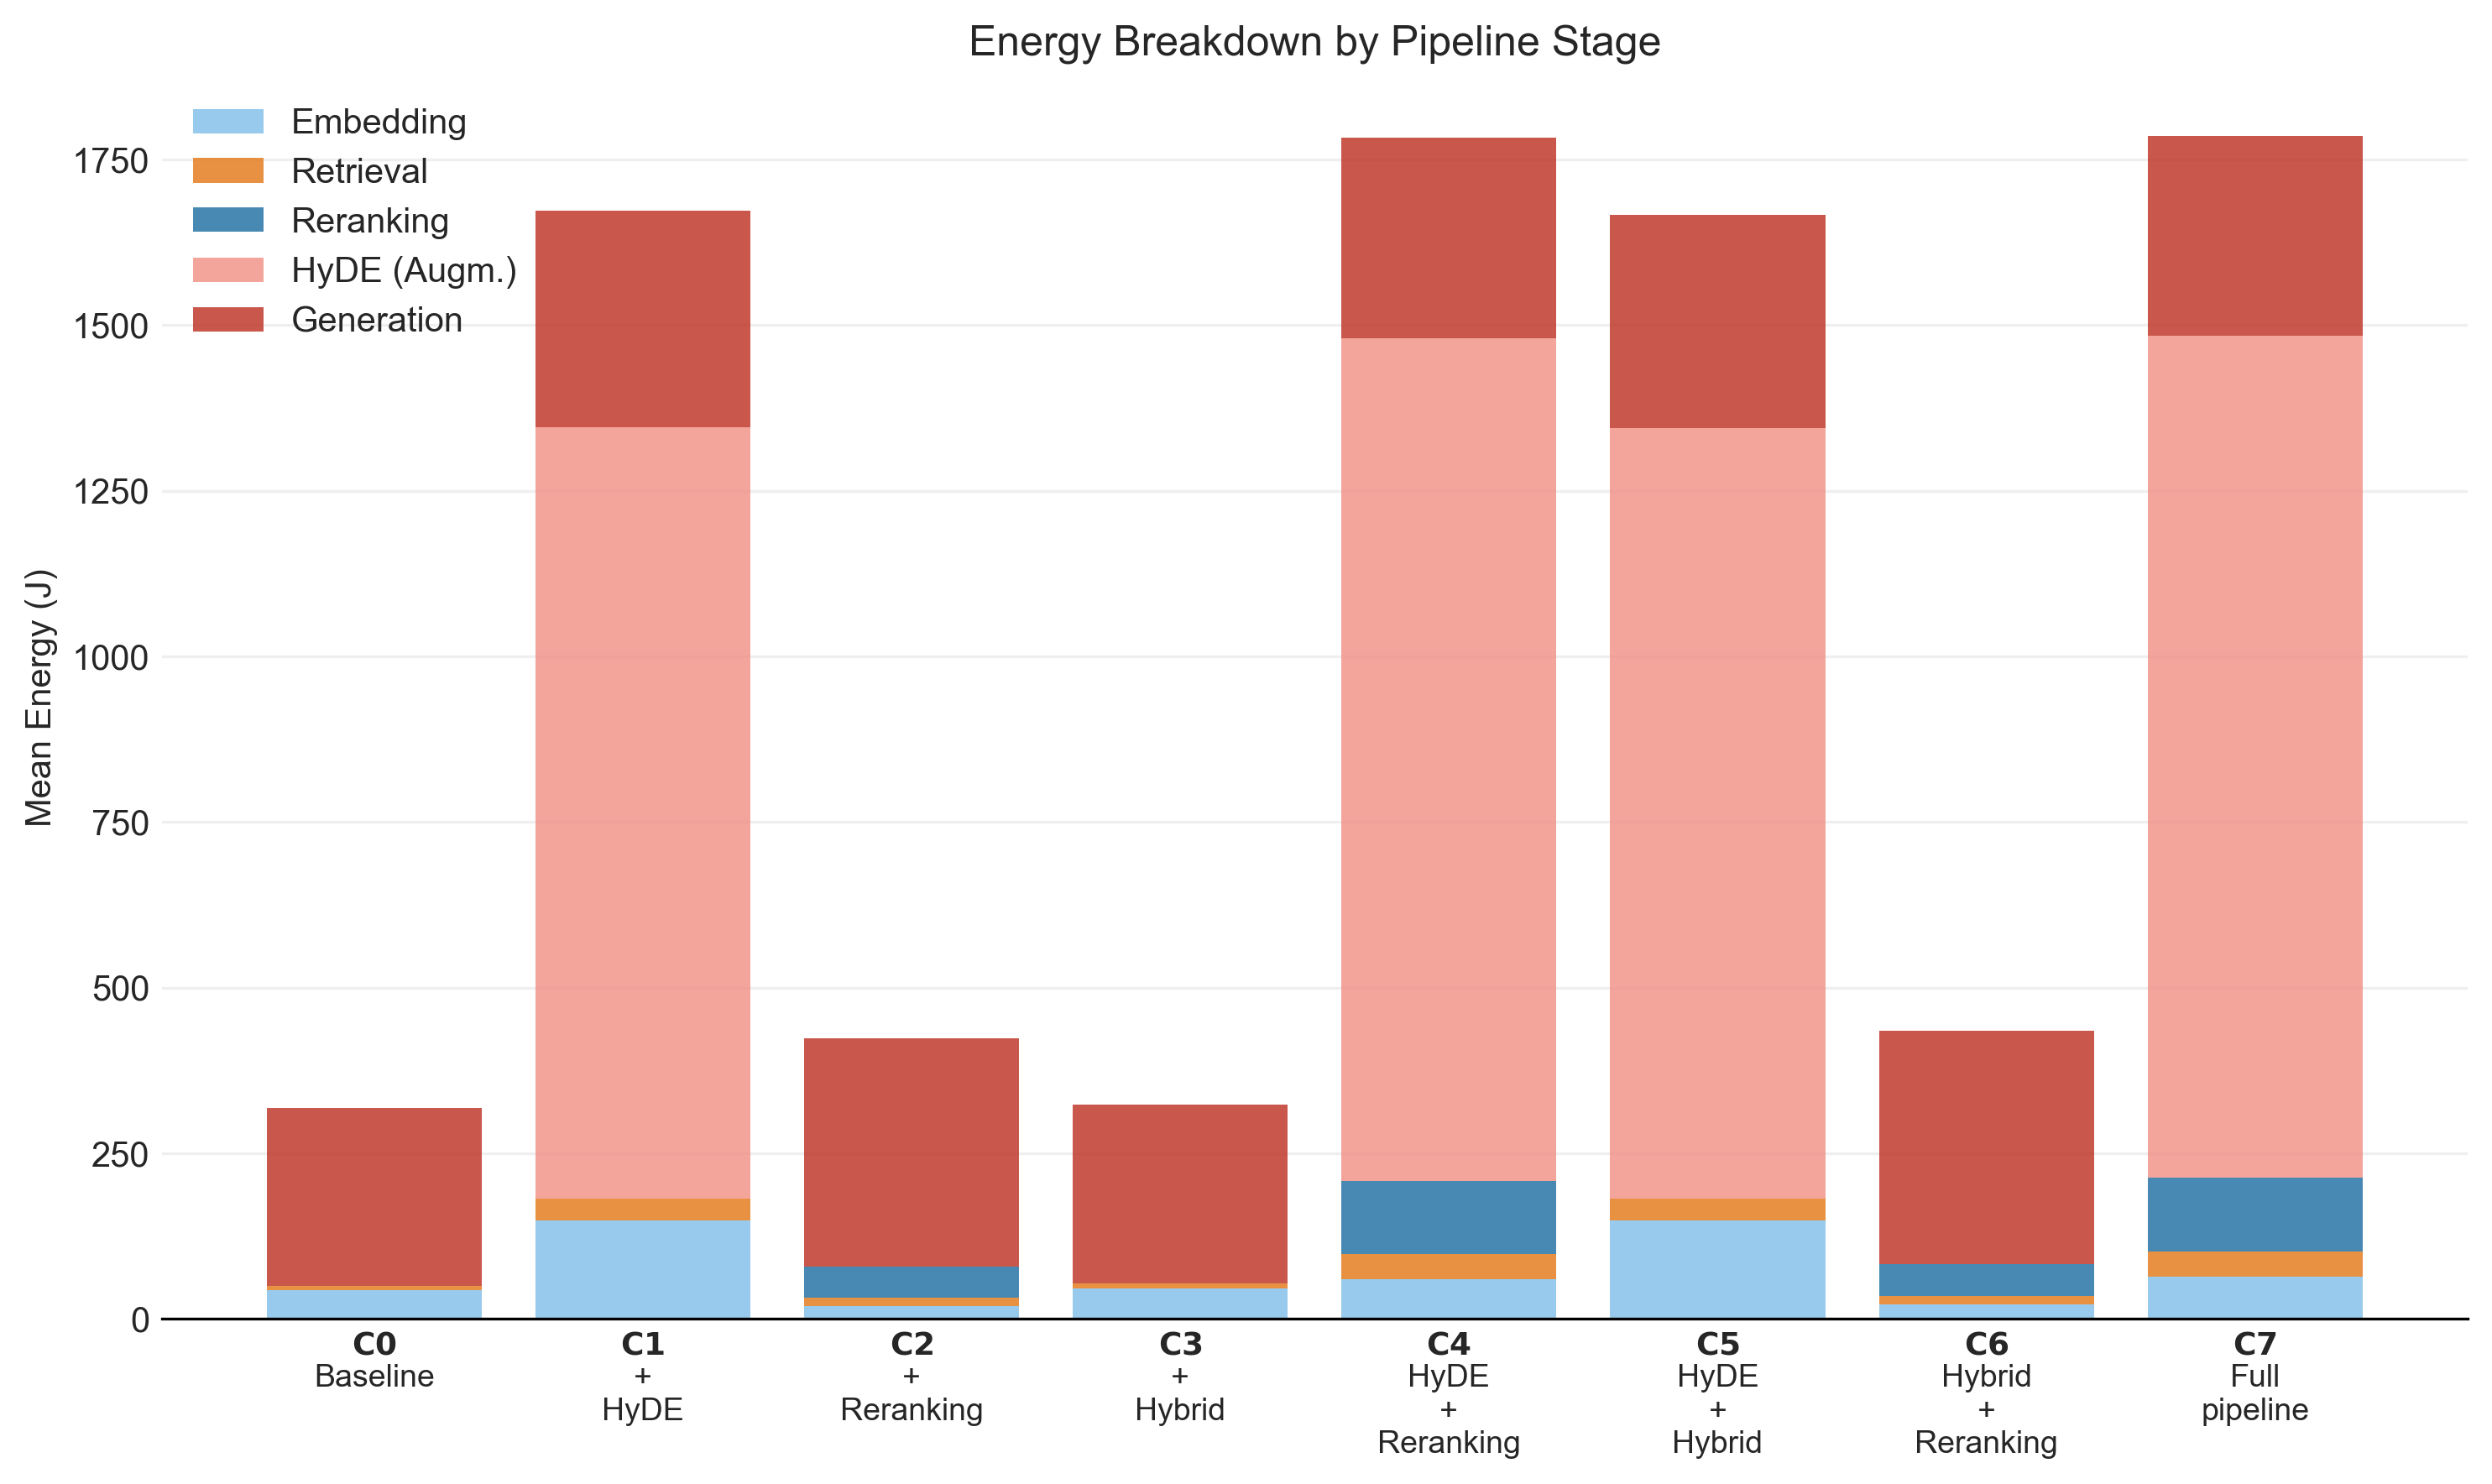
\includegraphics[width=0.85\textwidth]{stage_energy_breakdown.png}
\caption{Stage-level energy waterfall}
\label{fig:app-stage-breakdown}
\end{figure}

\begin{figure}[H]
\centering
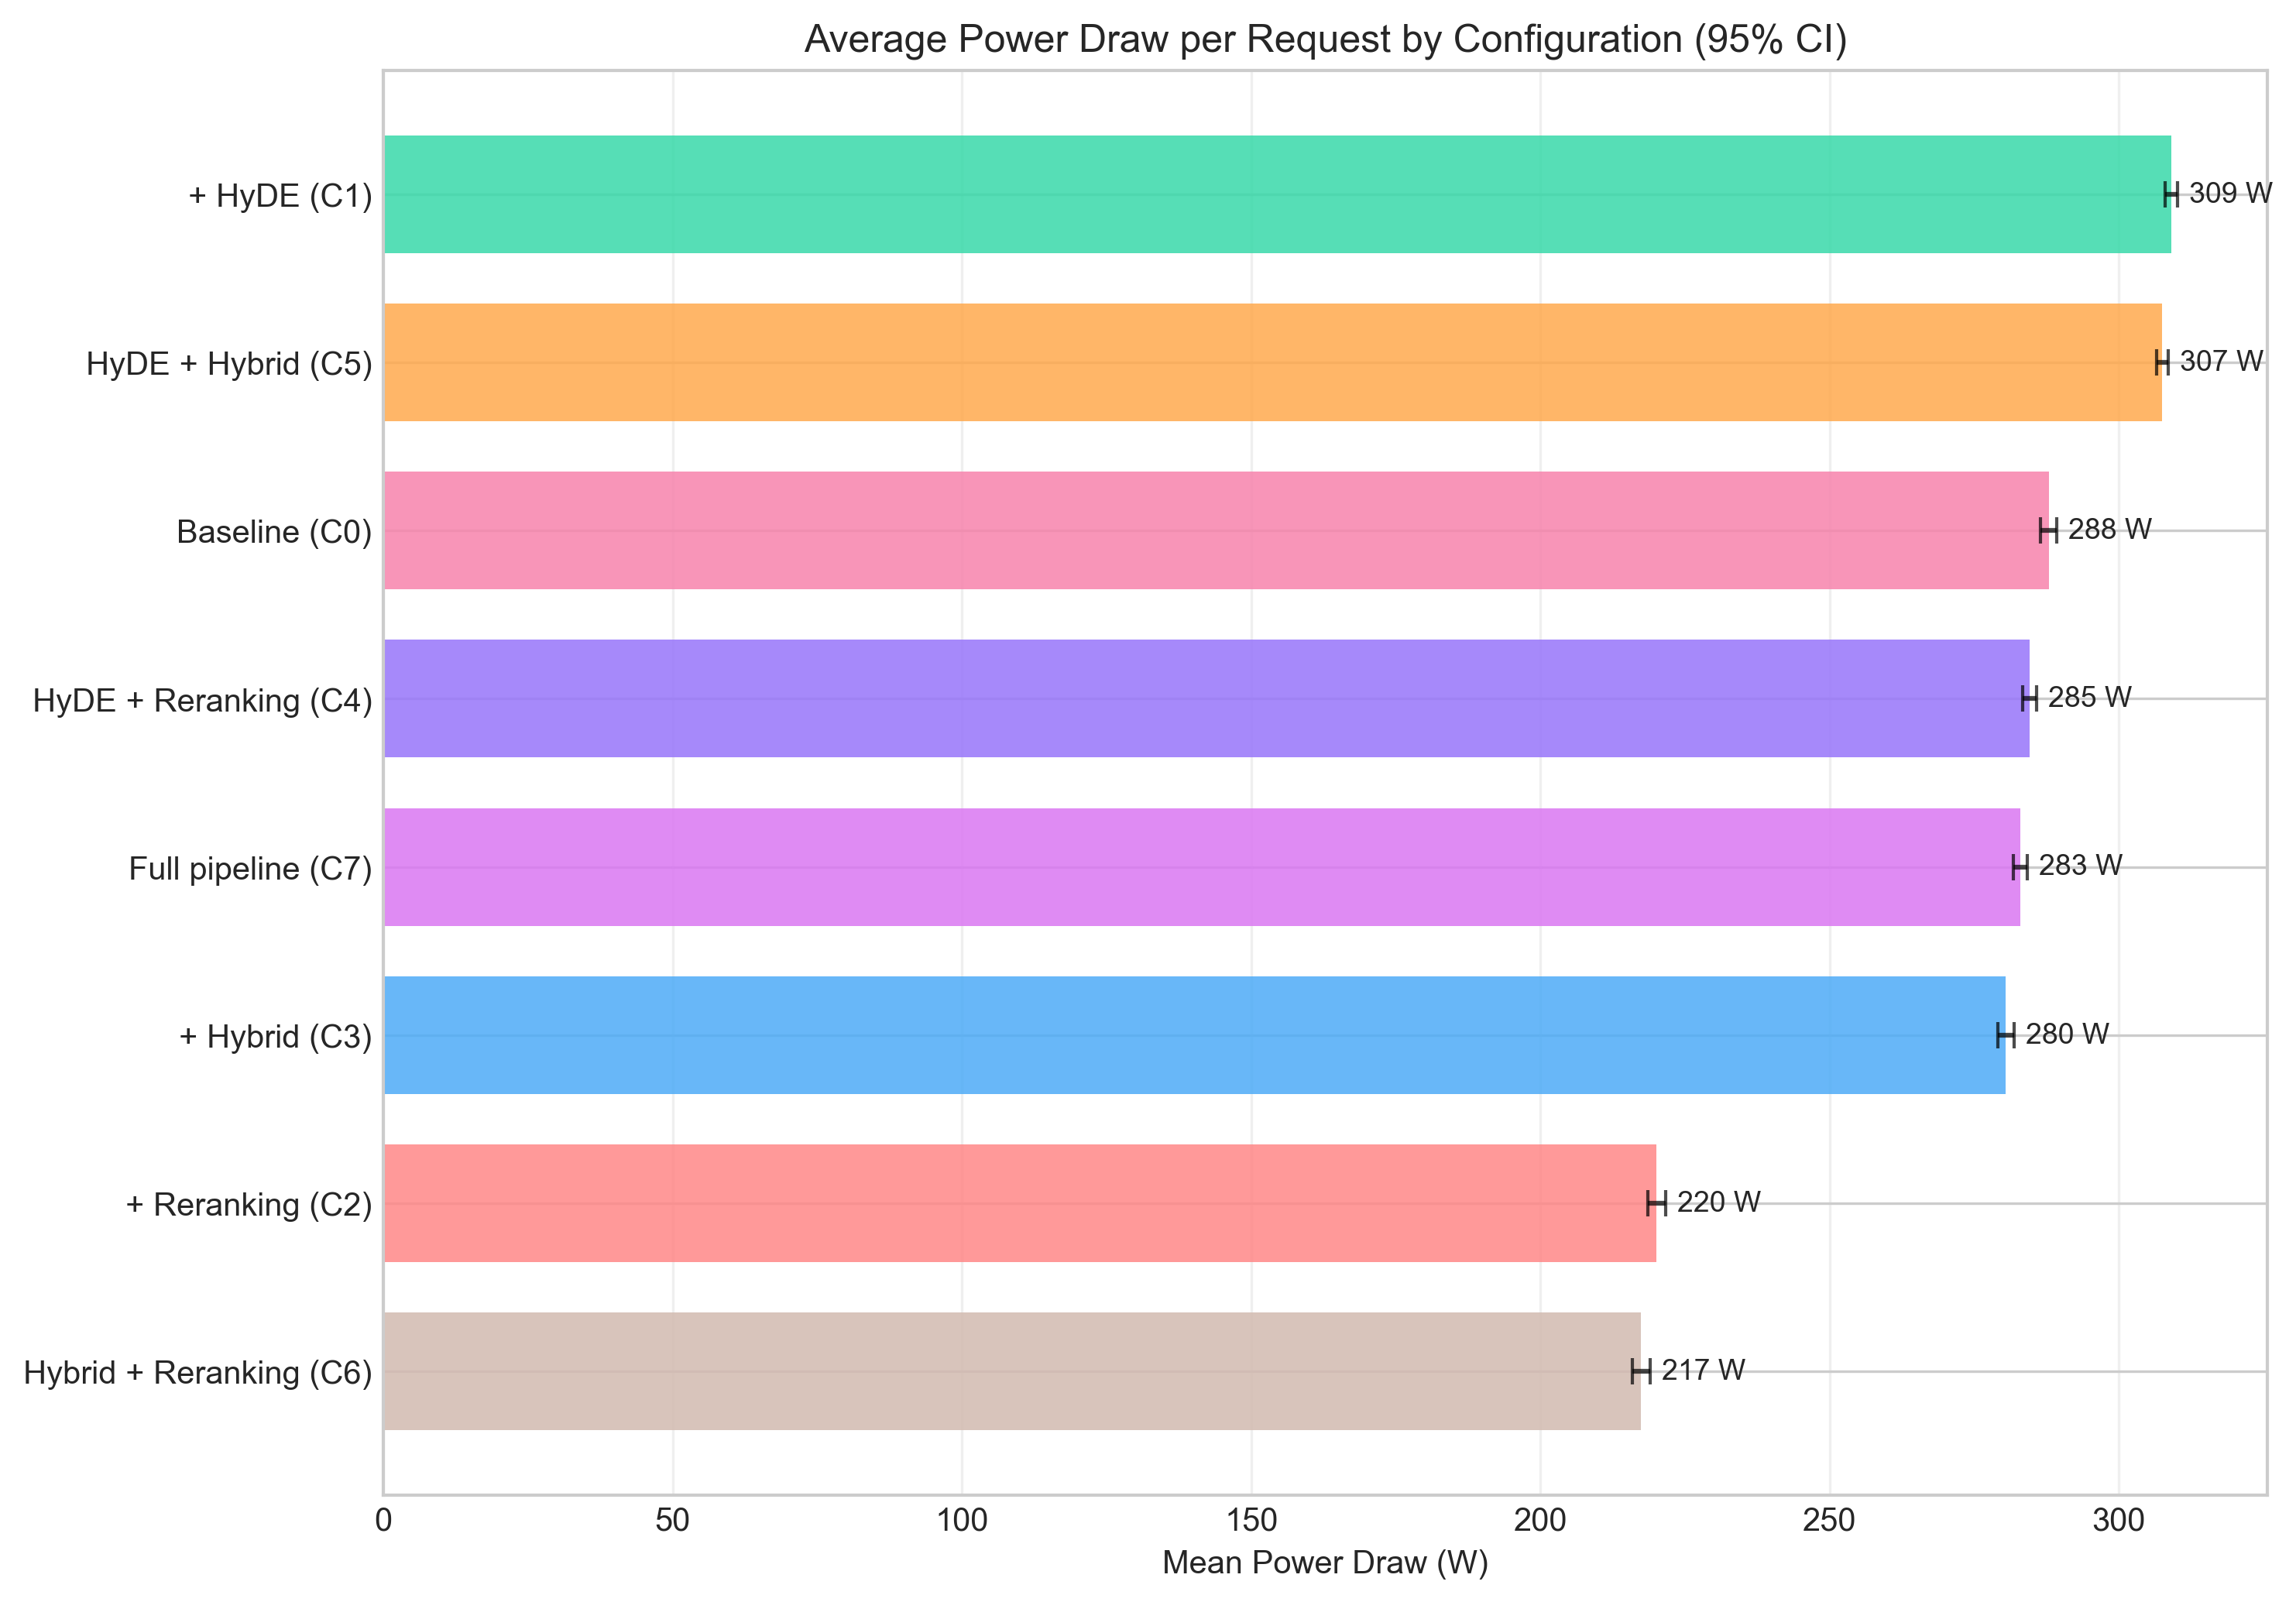
\includegraphics[width=0.85\textwidth]{power_draw_by_config.png}
\caption{Mean power draw by configuration}
\label{fig:app-power}
\end{figure}


% References
\newpage
\addcontentsline{toc}{section}{References}
\bibliographystyle{config/plain-nonote}
\bibliography{sections/refs.bib}

% Declaration of AI Tool Usage
\vspace{2cm}
\noindent\textbf{Declaration}
Large language model assistants (Claude, Deepl and Google) were used during the
preparation of this thesis for text translation and writing assistance
as linguistic refinement, including grammar correction, 
sentence rephrasing.  All research questions,
experimental designs, analyses and conclusions are the original work of
the author.

\end{document}
